\chapter{Entraînement de \textit{Shadow Models} sur des ensembles connus}\label{SM}
    Le Shadow Model n'est efficace que sous la condition d'adopter un comportement similaire à celui du modèle initial.

    Ce chapitre a donc pour but la détermination d'un ensemble $\mathbb{S}'_{Pri}$, composé du
    plus grand nombre possible de datasets d'entraînement de $\mathcal G$ notés $\mathbb{S}'_{Pri_i}$
    générant $\mathbb S_{Synth_i}'$ tel que :
                \begin{equation}\label{eq:Eq1}
                    \begin{split}
                        \mathbb{S}'_{Pri} &= \sum_i \mathbb{S}'_{Pri_i} \\
                        \forall i; \mathbb{S}'_{Pri_i} &\approxeq \mathbb{S}_{Pri}
                    \end{split}
                \end{equation}
                \myequations{Critère fondamental pour construire $\mathbb{S}'_{Pri}$}
    Rappelons que $\mathbb{S}_{Pri}$ n'est pas connu \textit{a priori}.

    Ainsi, afin de garantir l'équivalence entre les deux modèles, un critère de sélection est
    adopté :
    \textbf{l'équipe fait l'hypothèse forte que pour une paire de modèles, une similarité entre les données de sortie suffit à prouver une similarité entre les données d'entraînement.}. Ainsi :
        \begin{equation}\label{eq:Eq2}
            \mathbb{S}'_{Pri_i} \approxeq \mathbb{S}_{Pri} \Longleftrightarrow \mathbb{S}'_{Synth_i} \approxeq \mathbb{S}_{Synth}
        \end{equation}
        \myequations{Hypothèse fondamentale pour construire $\mathbb{S}'_{Pri}$}

    \begin{tcolorbox}[colback=linkborder_Color!5!white,colframe=linkborder_Color!75!black]
        Ainsi, au-dela de la performance du modèle de classification, deux paramètres essentiels
        doivent retenir l'attention :

        \begin{itemize}
            \item La taille du dataset d'entraînement $l\left(\mathcal S'_{pri}\right)$
            \item La similarité entre $\mathbb{S}'_{Synth_i}$ et $\mathbb{S}_{Synth}$
        \end{itemize}
    \end{tcolorbox}

        Les sections suivantes proposent plusieurs approches avec différentes prises en compte de
        ces paramètres.
    \section{Essai préliminaire avec un seul dataset $\left(E_{T_2, \overline C, l_{2}}\right)$}

        Cette expérience sert avant tout à construire un framework d'étude et à appréhender les
        différentes composantes du problème. C'est celle-ci qui a été présentée lors de la
        restitution à mi-parcours du projet.

        L'objectif est d'établir un point de départ sur lequel articuler des réflexions plus
        poussées. On choisit donc d'entraîner le classifieur sur un seul dataset
        $\mathbb S'_{priv} | l\left( \mathbb{S}'_{priv} = 1000 \right)$. Ce dataset privé est
        obtenu en changeant la seed générative du DopelGanger.

        \begin{tcolorbox}[colback=linkborder_Color!5!white,colframe=linkborder_Color!75!black]
            Cette première expérience permet d'obtenir $\mathtt S_{T_2}=0,47$. Ce score
            largement perfectible est partiellement du à un mauvais classifieur, mais son
            principal problème est un nombre trop faible de lignes. Les expériences suivantes
            cherchent donc à augmenter $l\left( \mathbb S'_{priv} \right)$ en créant plus de
            Shadow Models.
        \end{tcolorbox}
    \newpage\section{Regroupement de plusieurs datasets pour augmenter la taille du dataset
d'entraînement $\left(E_{T_2, \overline C, l_{30}}\right)$}
        Cette opération est similaire à la première, mais on cherche à maximiser $l\left( \mathbb S'_{priv} \right)$
        pour faciliter l'entraînement du classifieur. Ainsi on construit 15 Shadows Models
        constitués chacun d'une paire $\mathbb{S}'_{priv_i}\longrightarrow \mathbb{S}'_{synth_i}$.

        \textit{Nb : On obtient $\mathbb{S}'_{priv_i}$ en changeant la seed générative de $\mathcal G$.}

        \begin{figure}[H]
            \centering
            \subfloat[]{\fbox{
                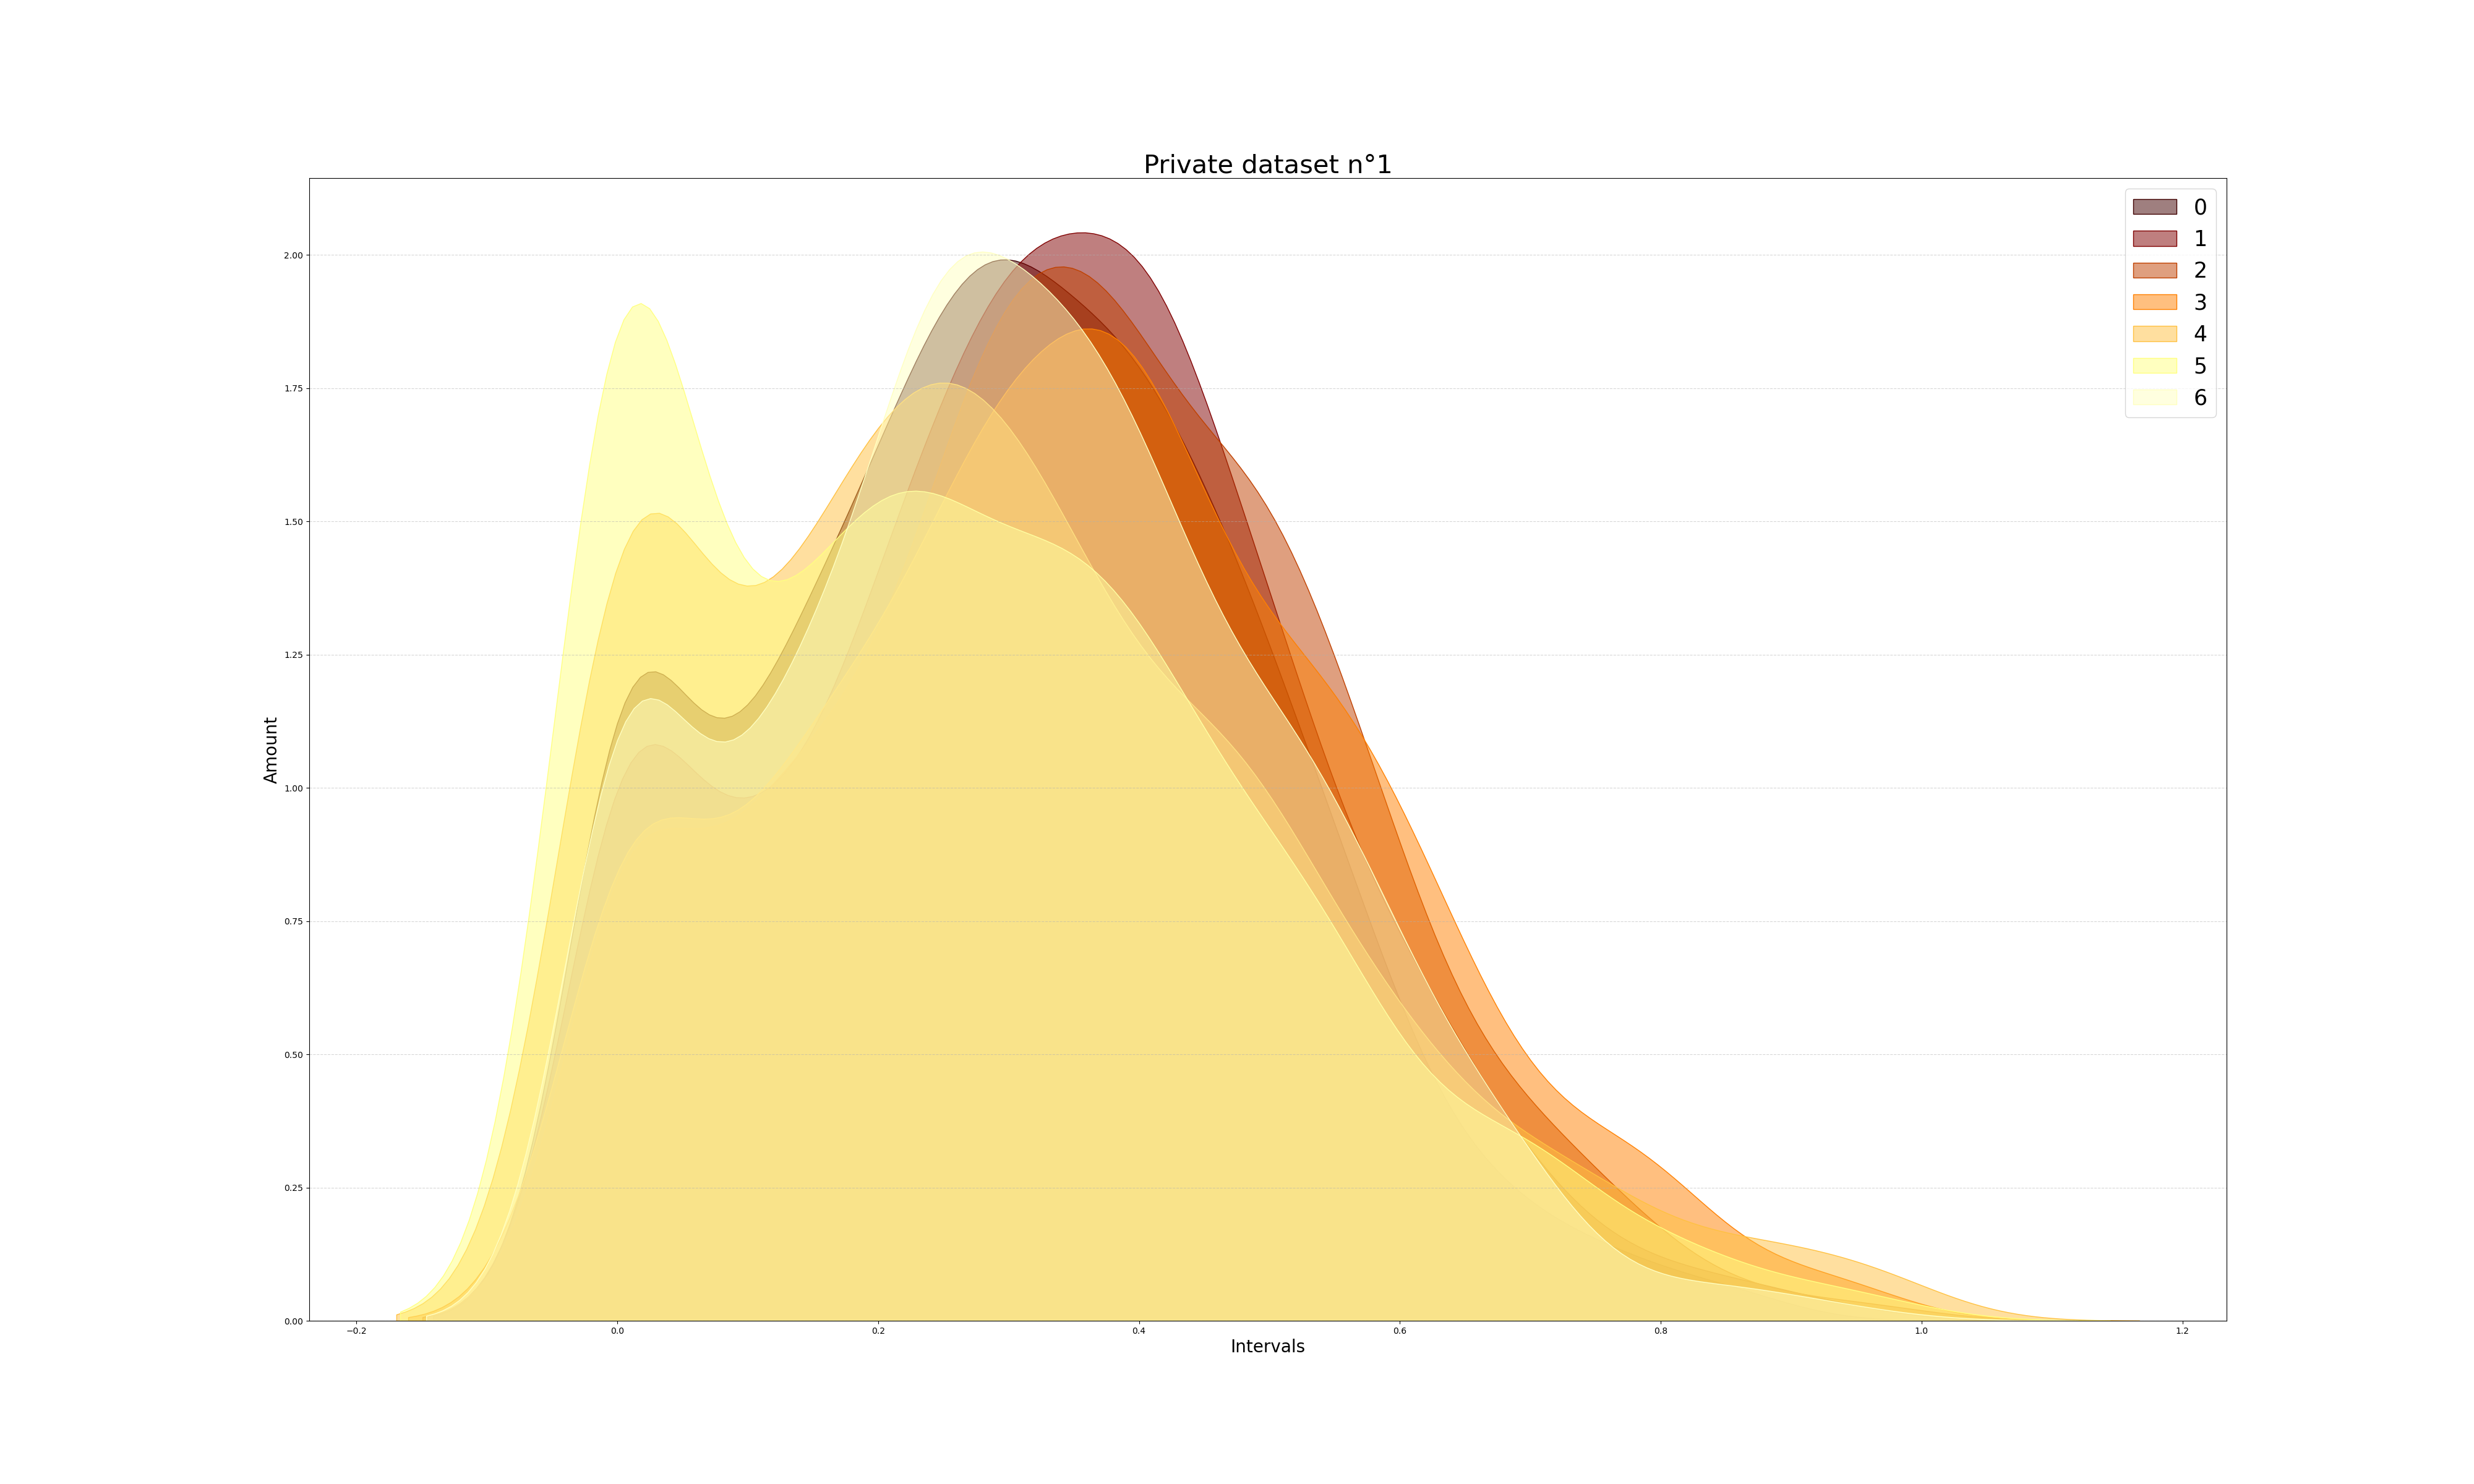
\includegraphics[width = 0.28\textwidth]{figures/Resultats/privateDS/Task 2/1}}}\qquad
            \subfloat[]{\fbox{
                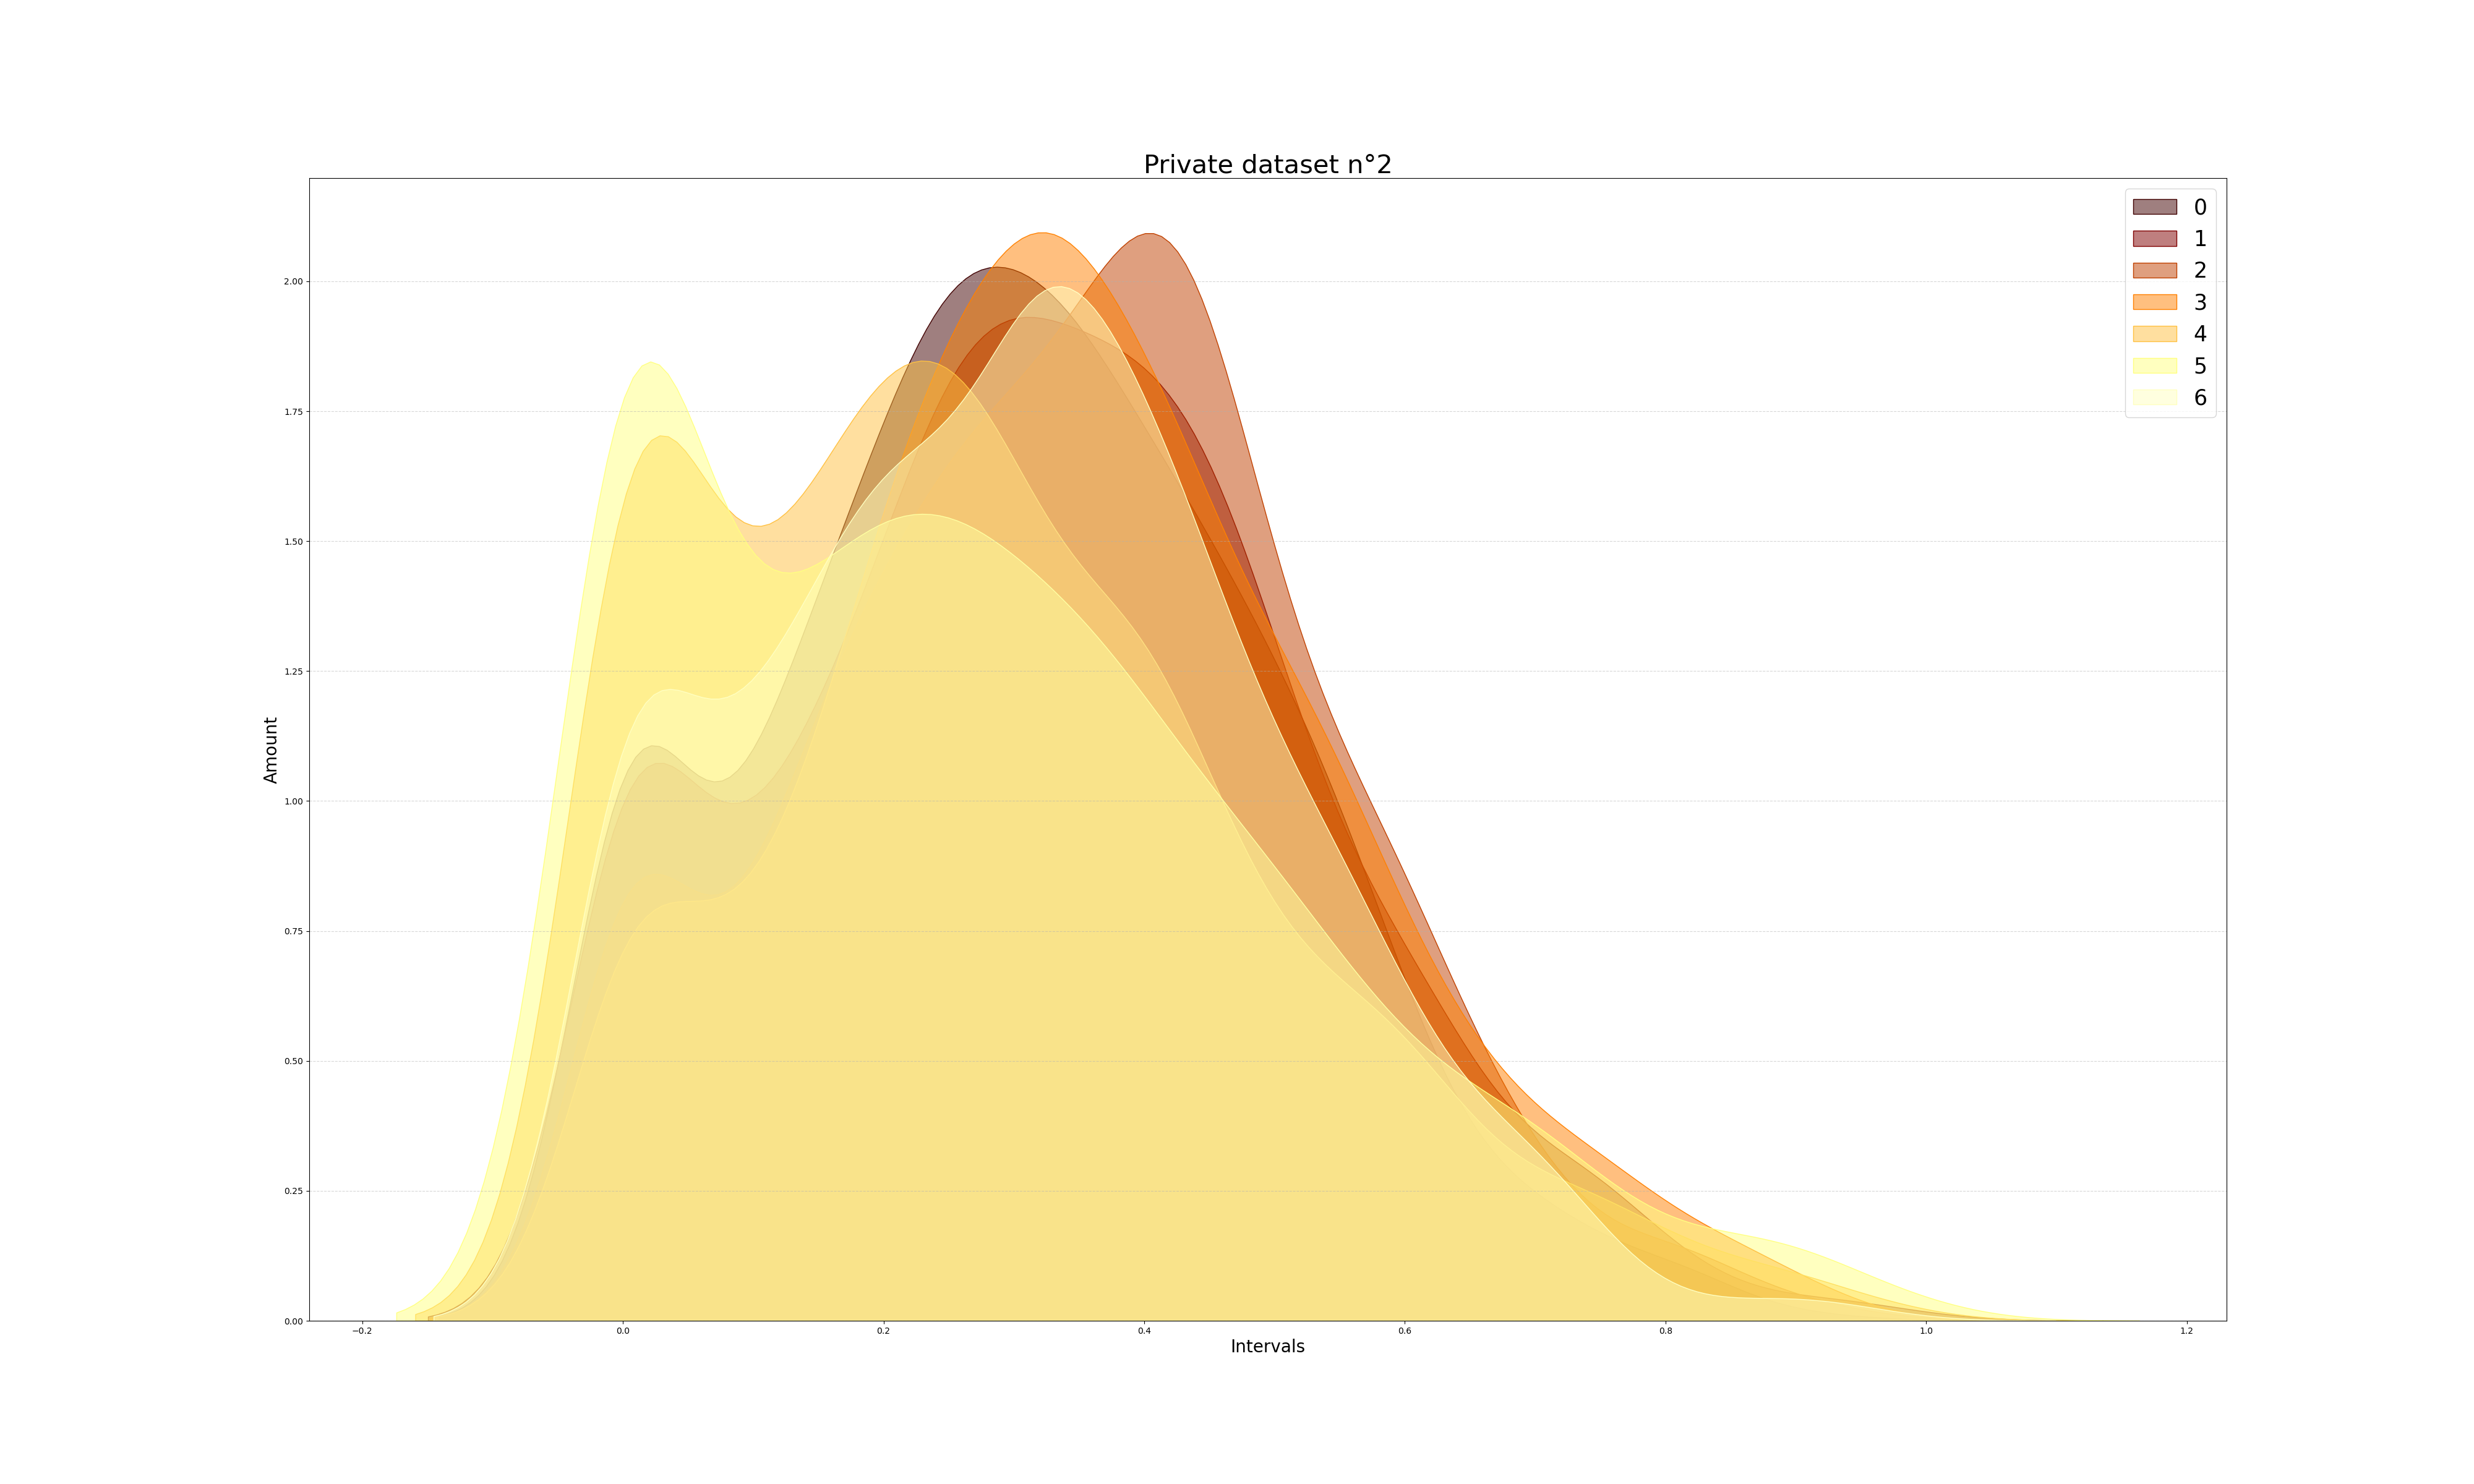
\includegraphics[width = 0.28\textwidth]{figures/Resultats/privateDS/Task 2/2}}}\qquad
            \subfloat[]{\fbox{
                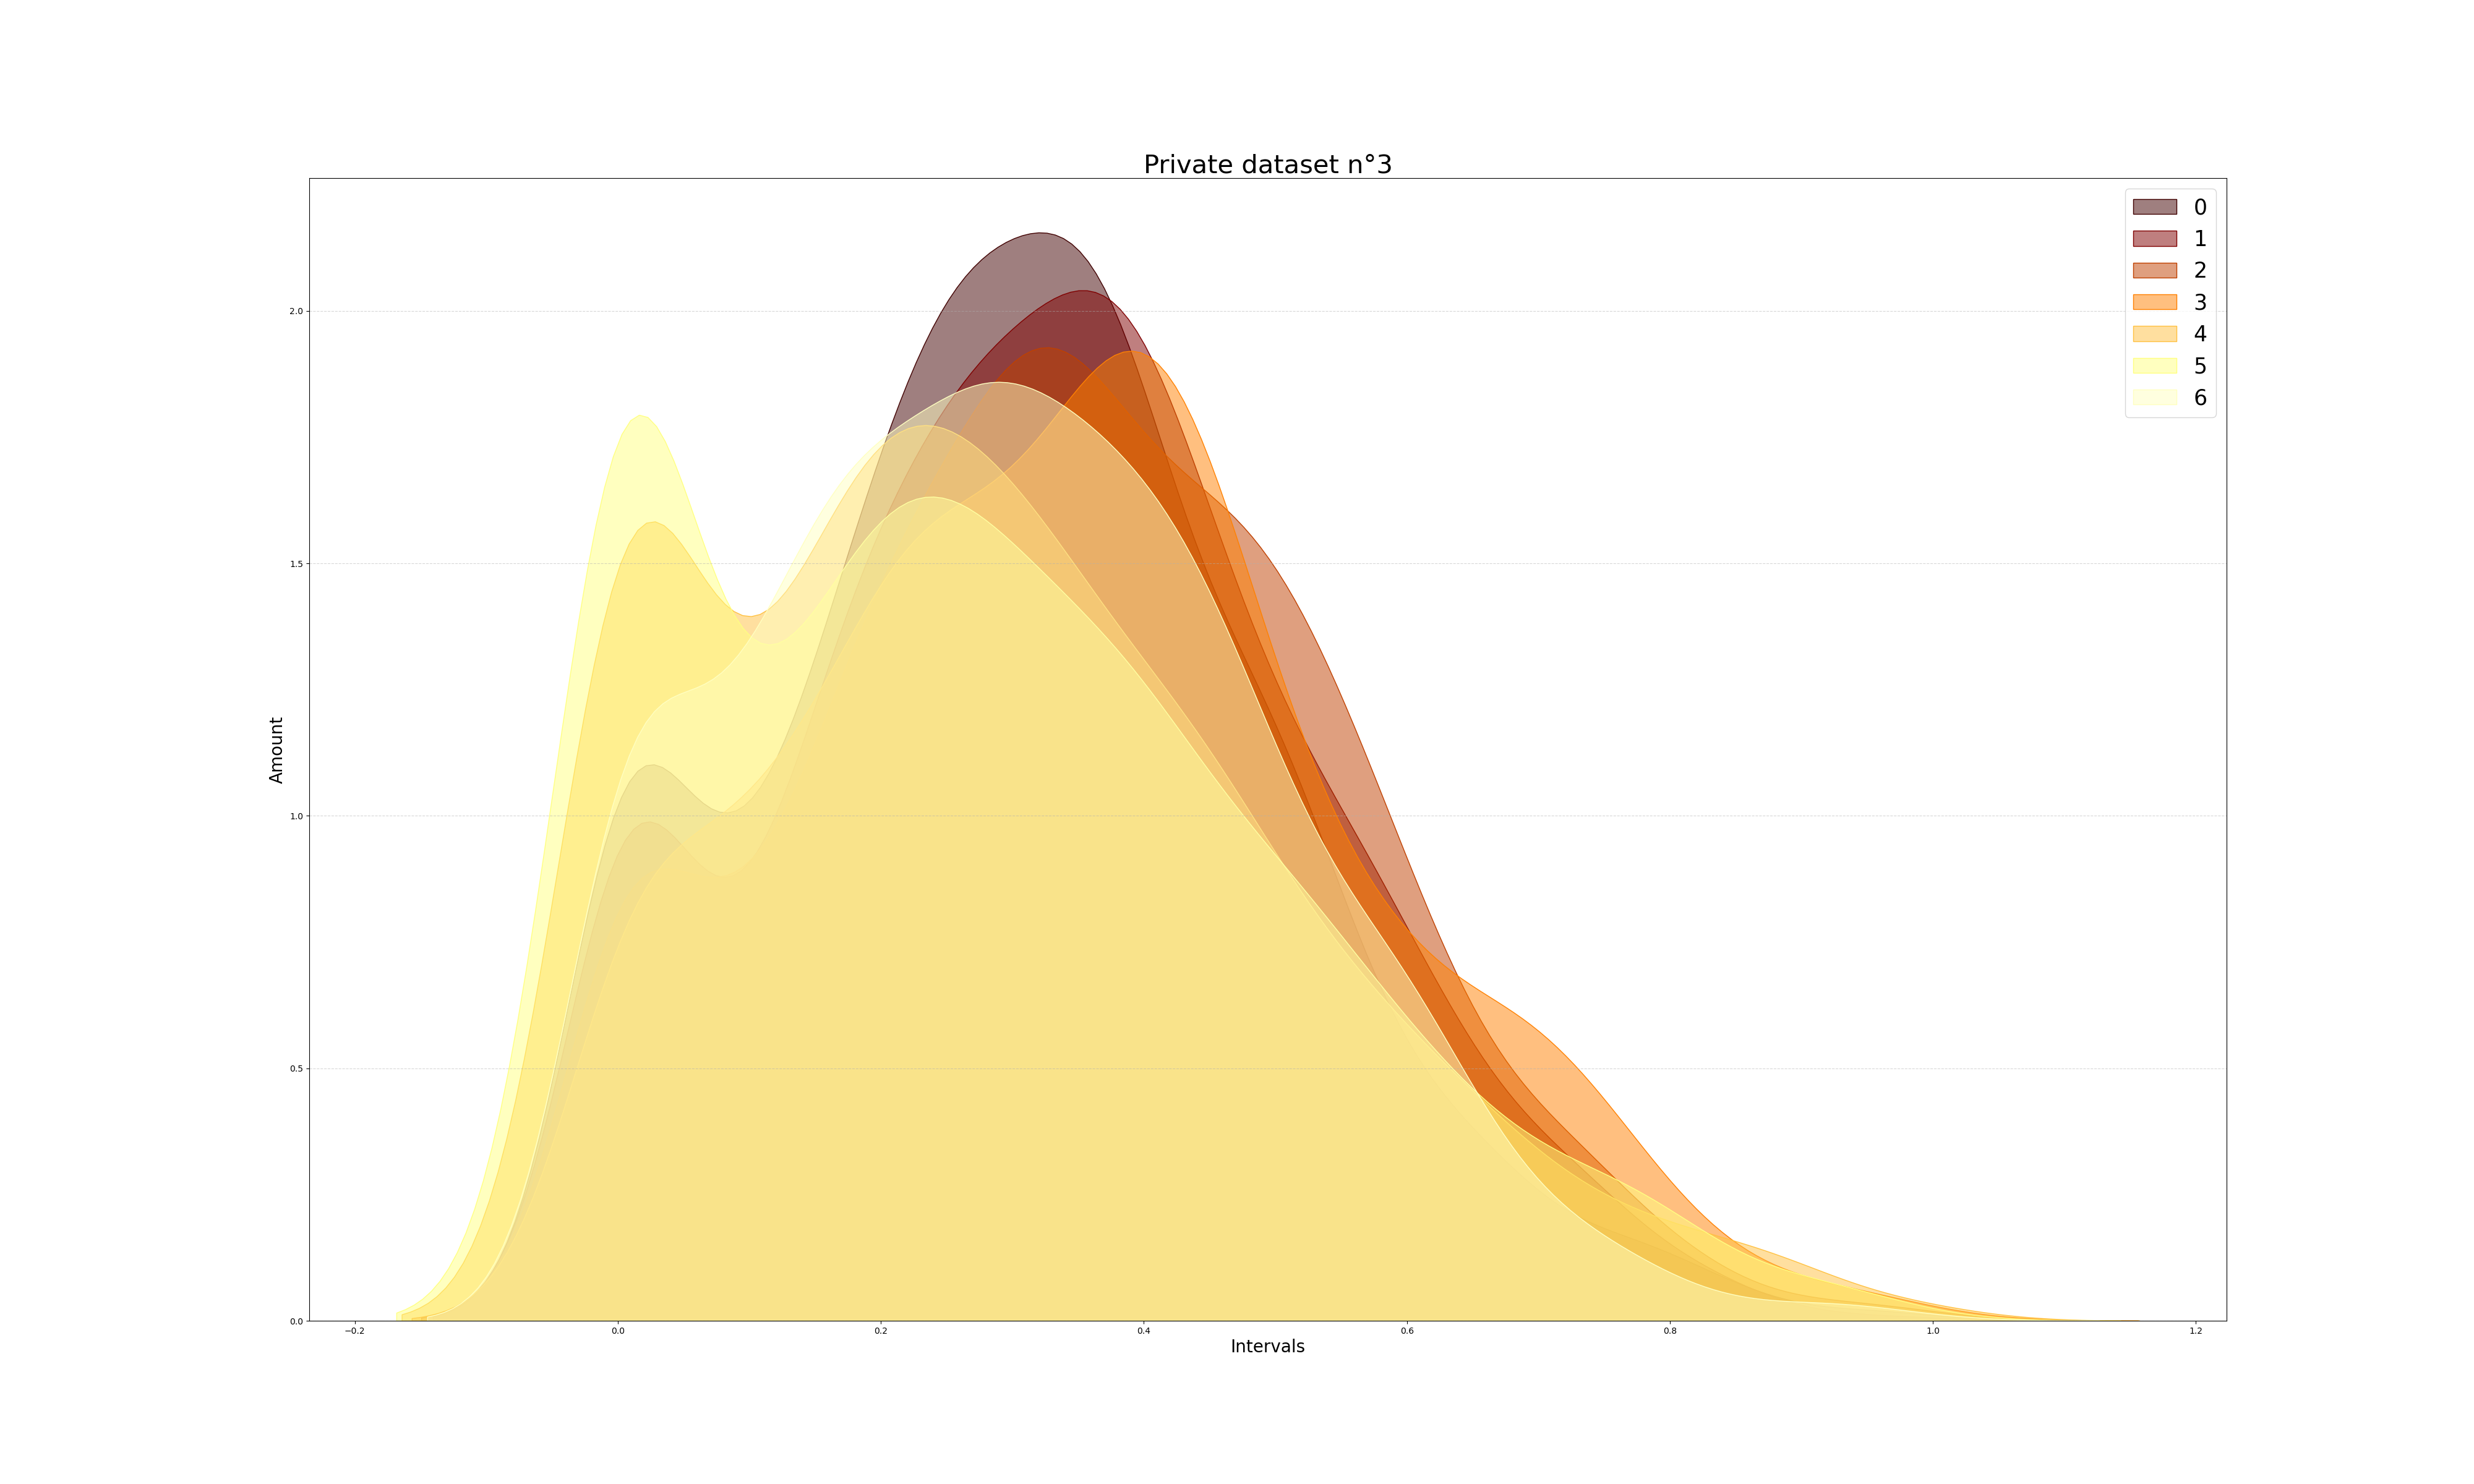
\includegraphics[width = 0.28\textwidth]{figures/Resultats/privateDS/Task 2/3}}}\qquad
            \subfloat[]{\fbox{
                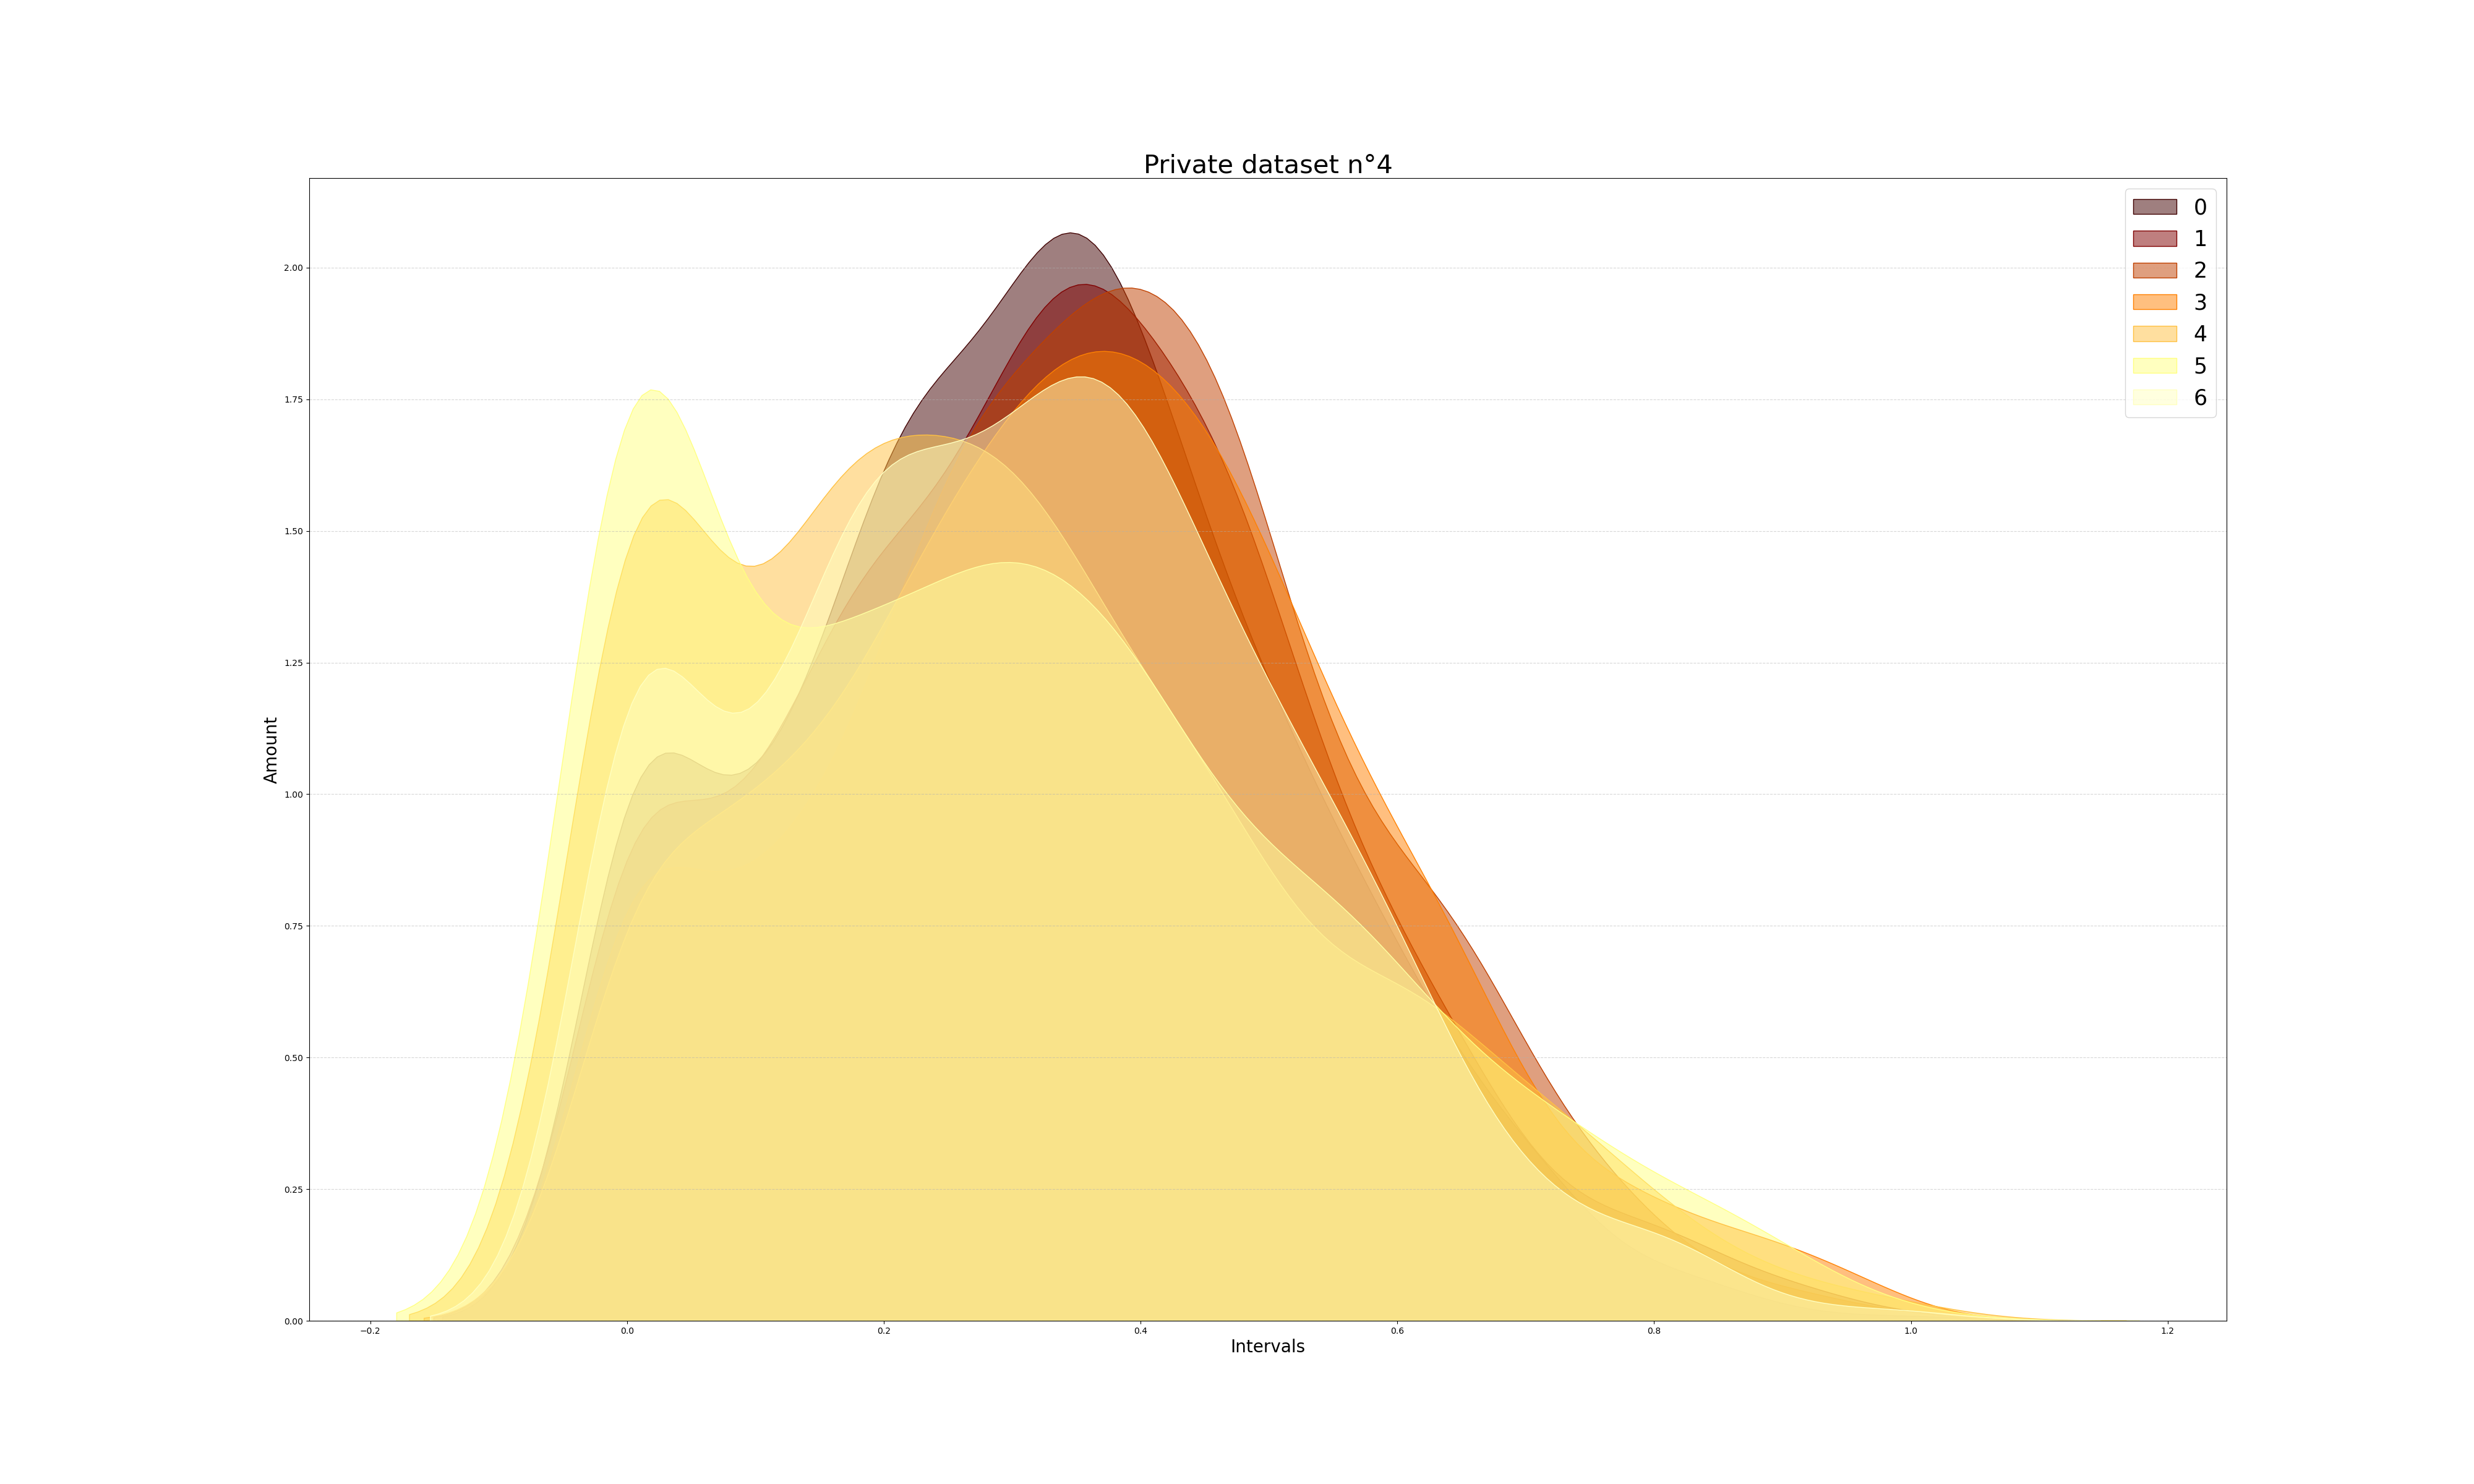
\includegraphics[width = 0.28\textwidth]{figures/Resultats/privateDS/Task 2/4}}}\qquad
            \subfloat[]{\fbox{
                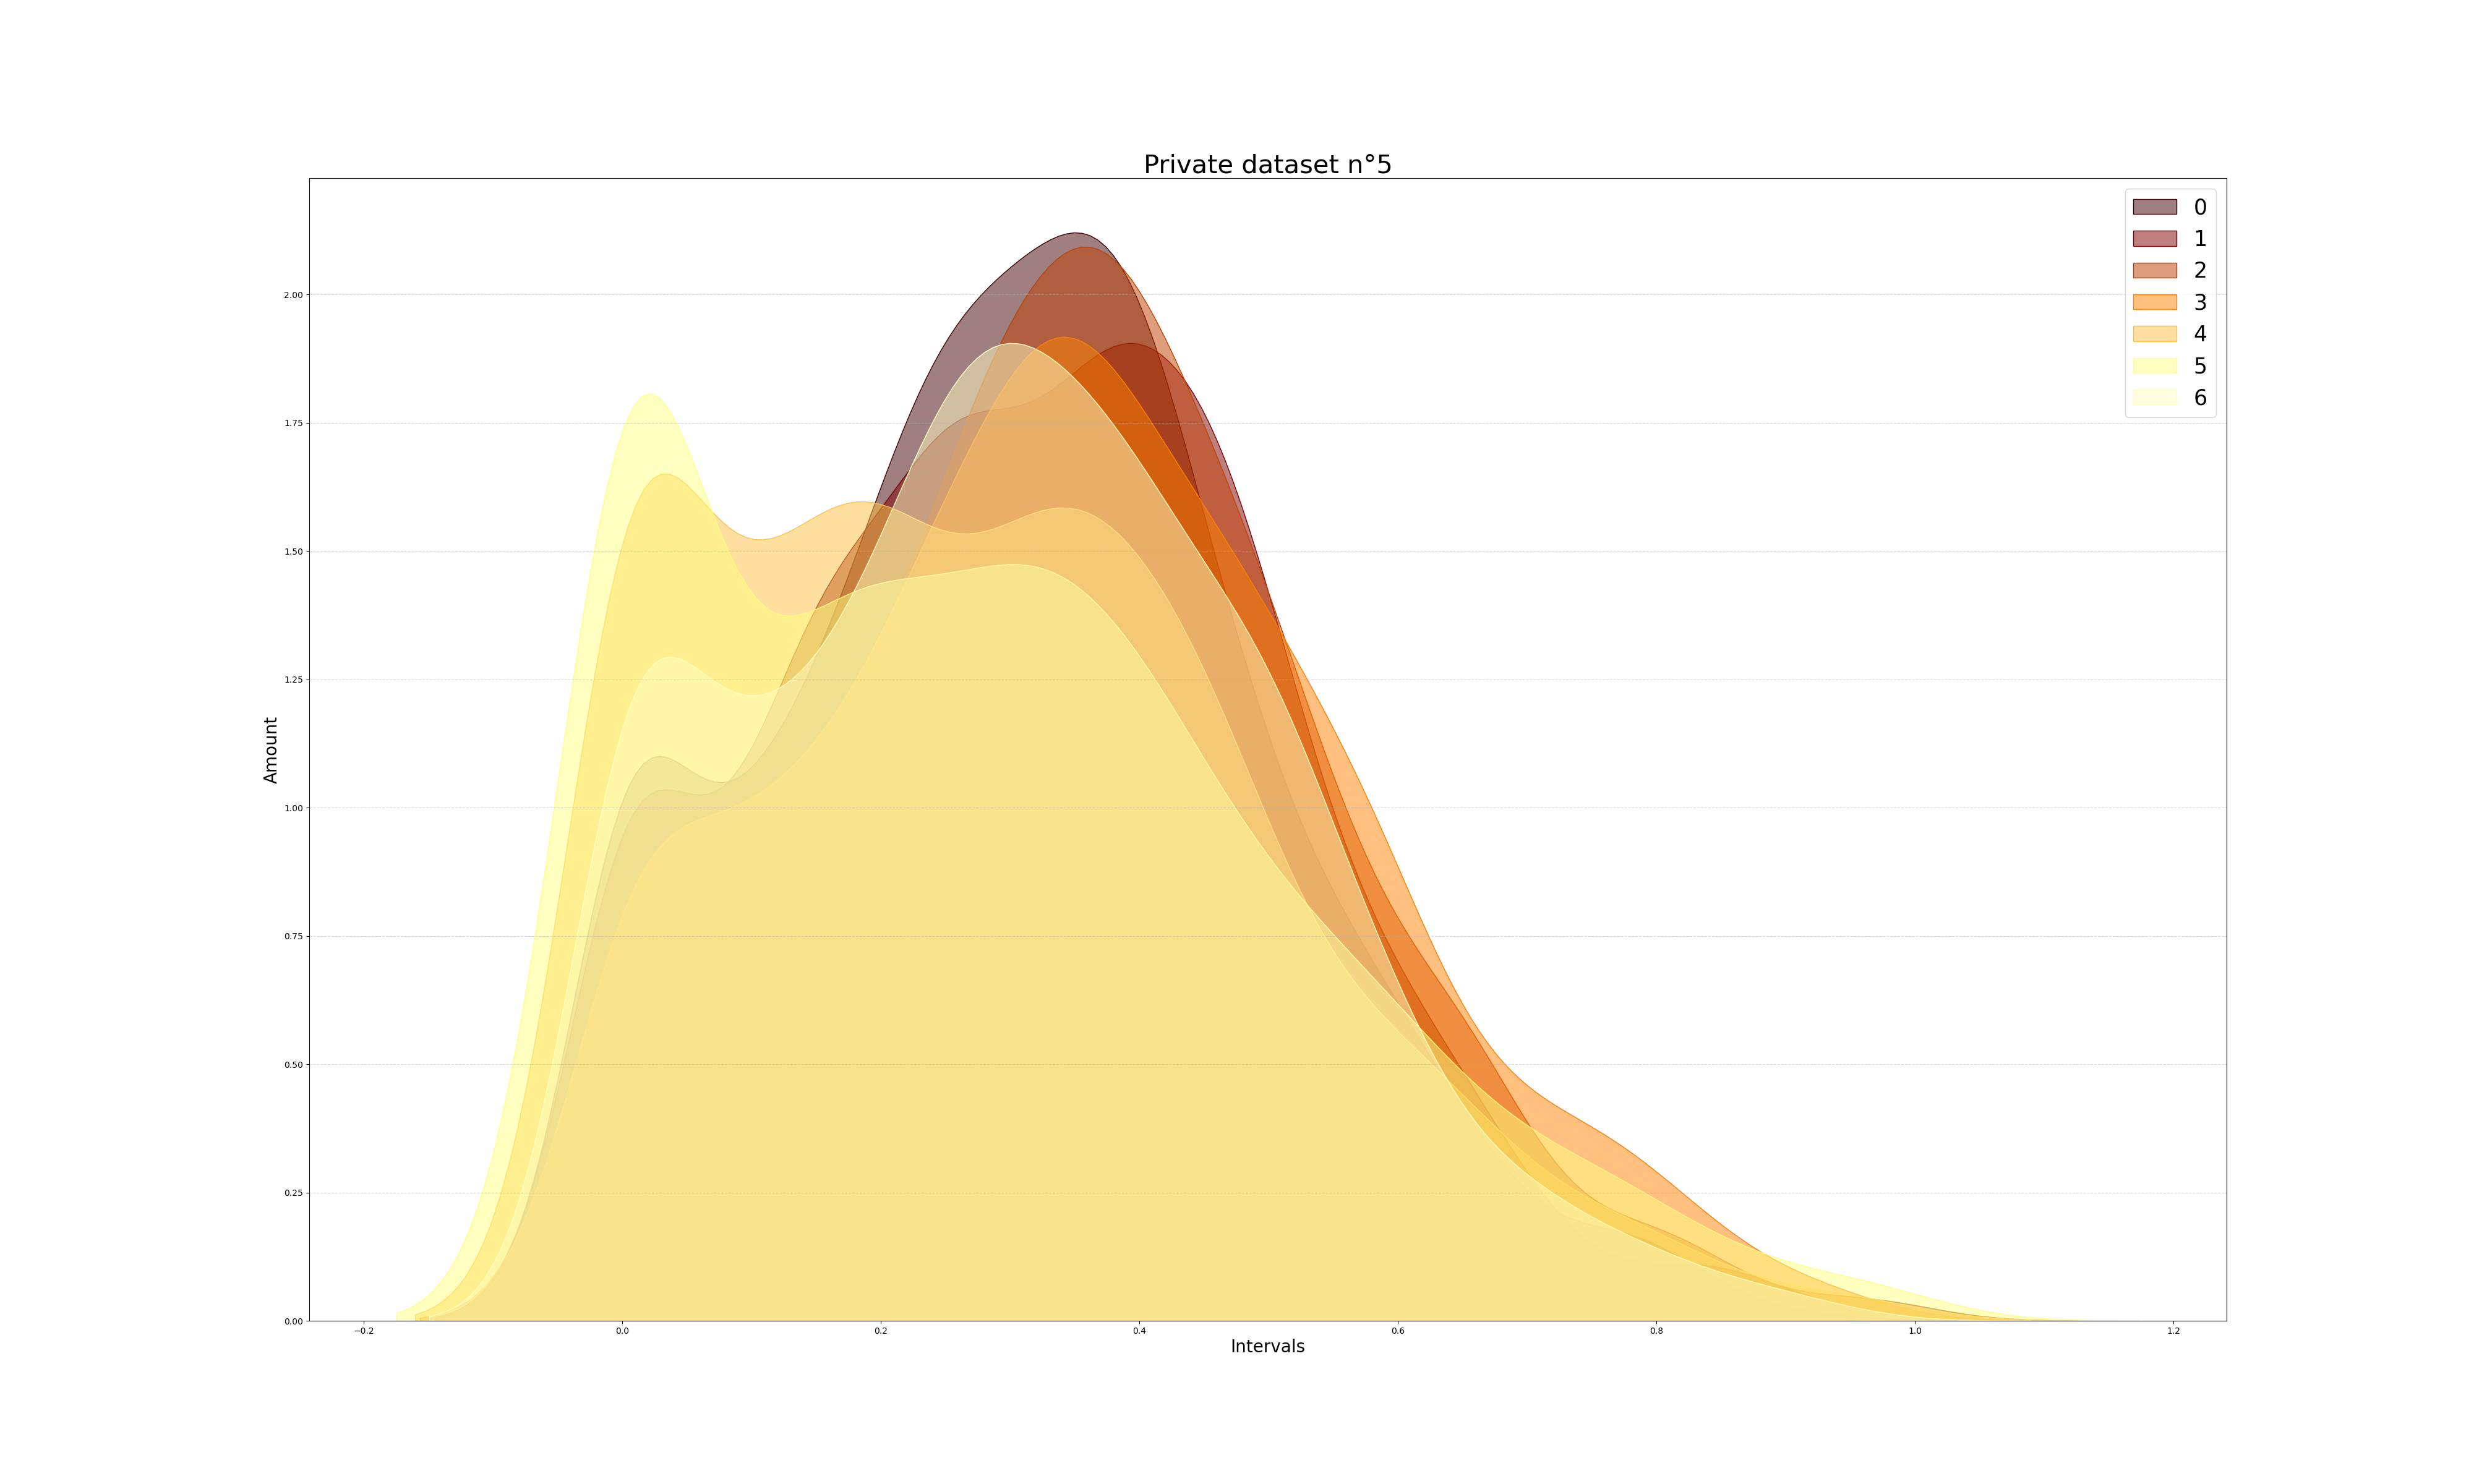
\includegraphics[width = 0.28\textwidth]{figures/Resultats/privateDS/Task 2/5}}}\qquad
            \subfloat[]{\fbox{
                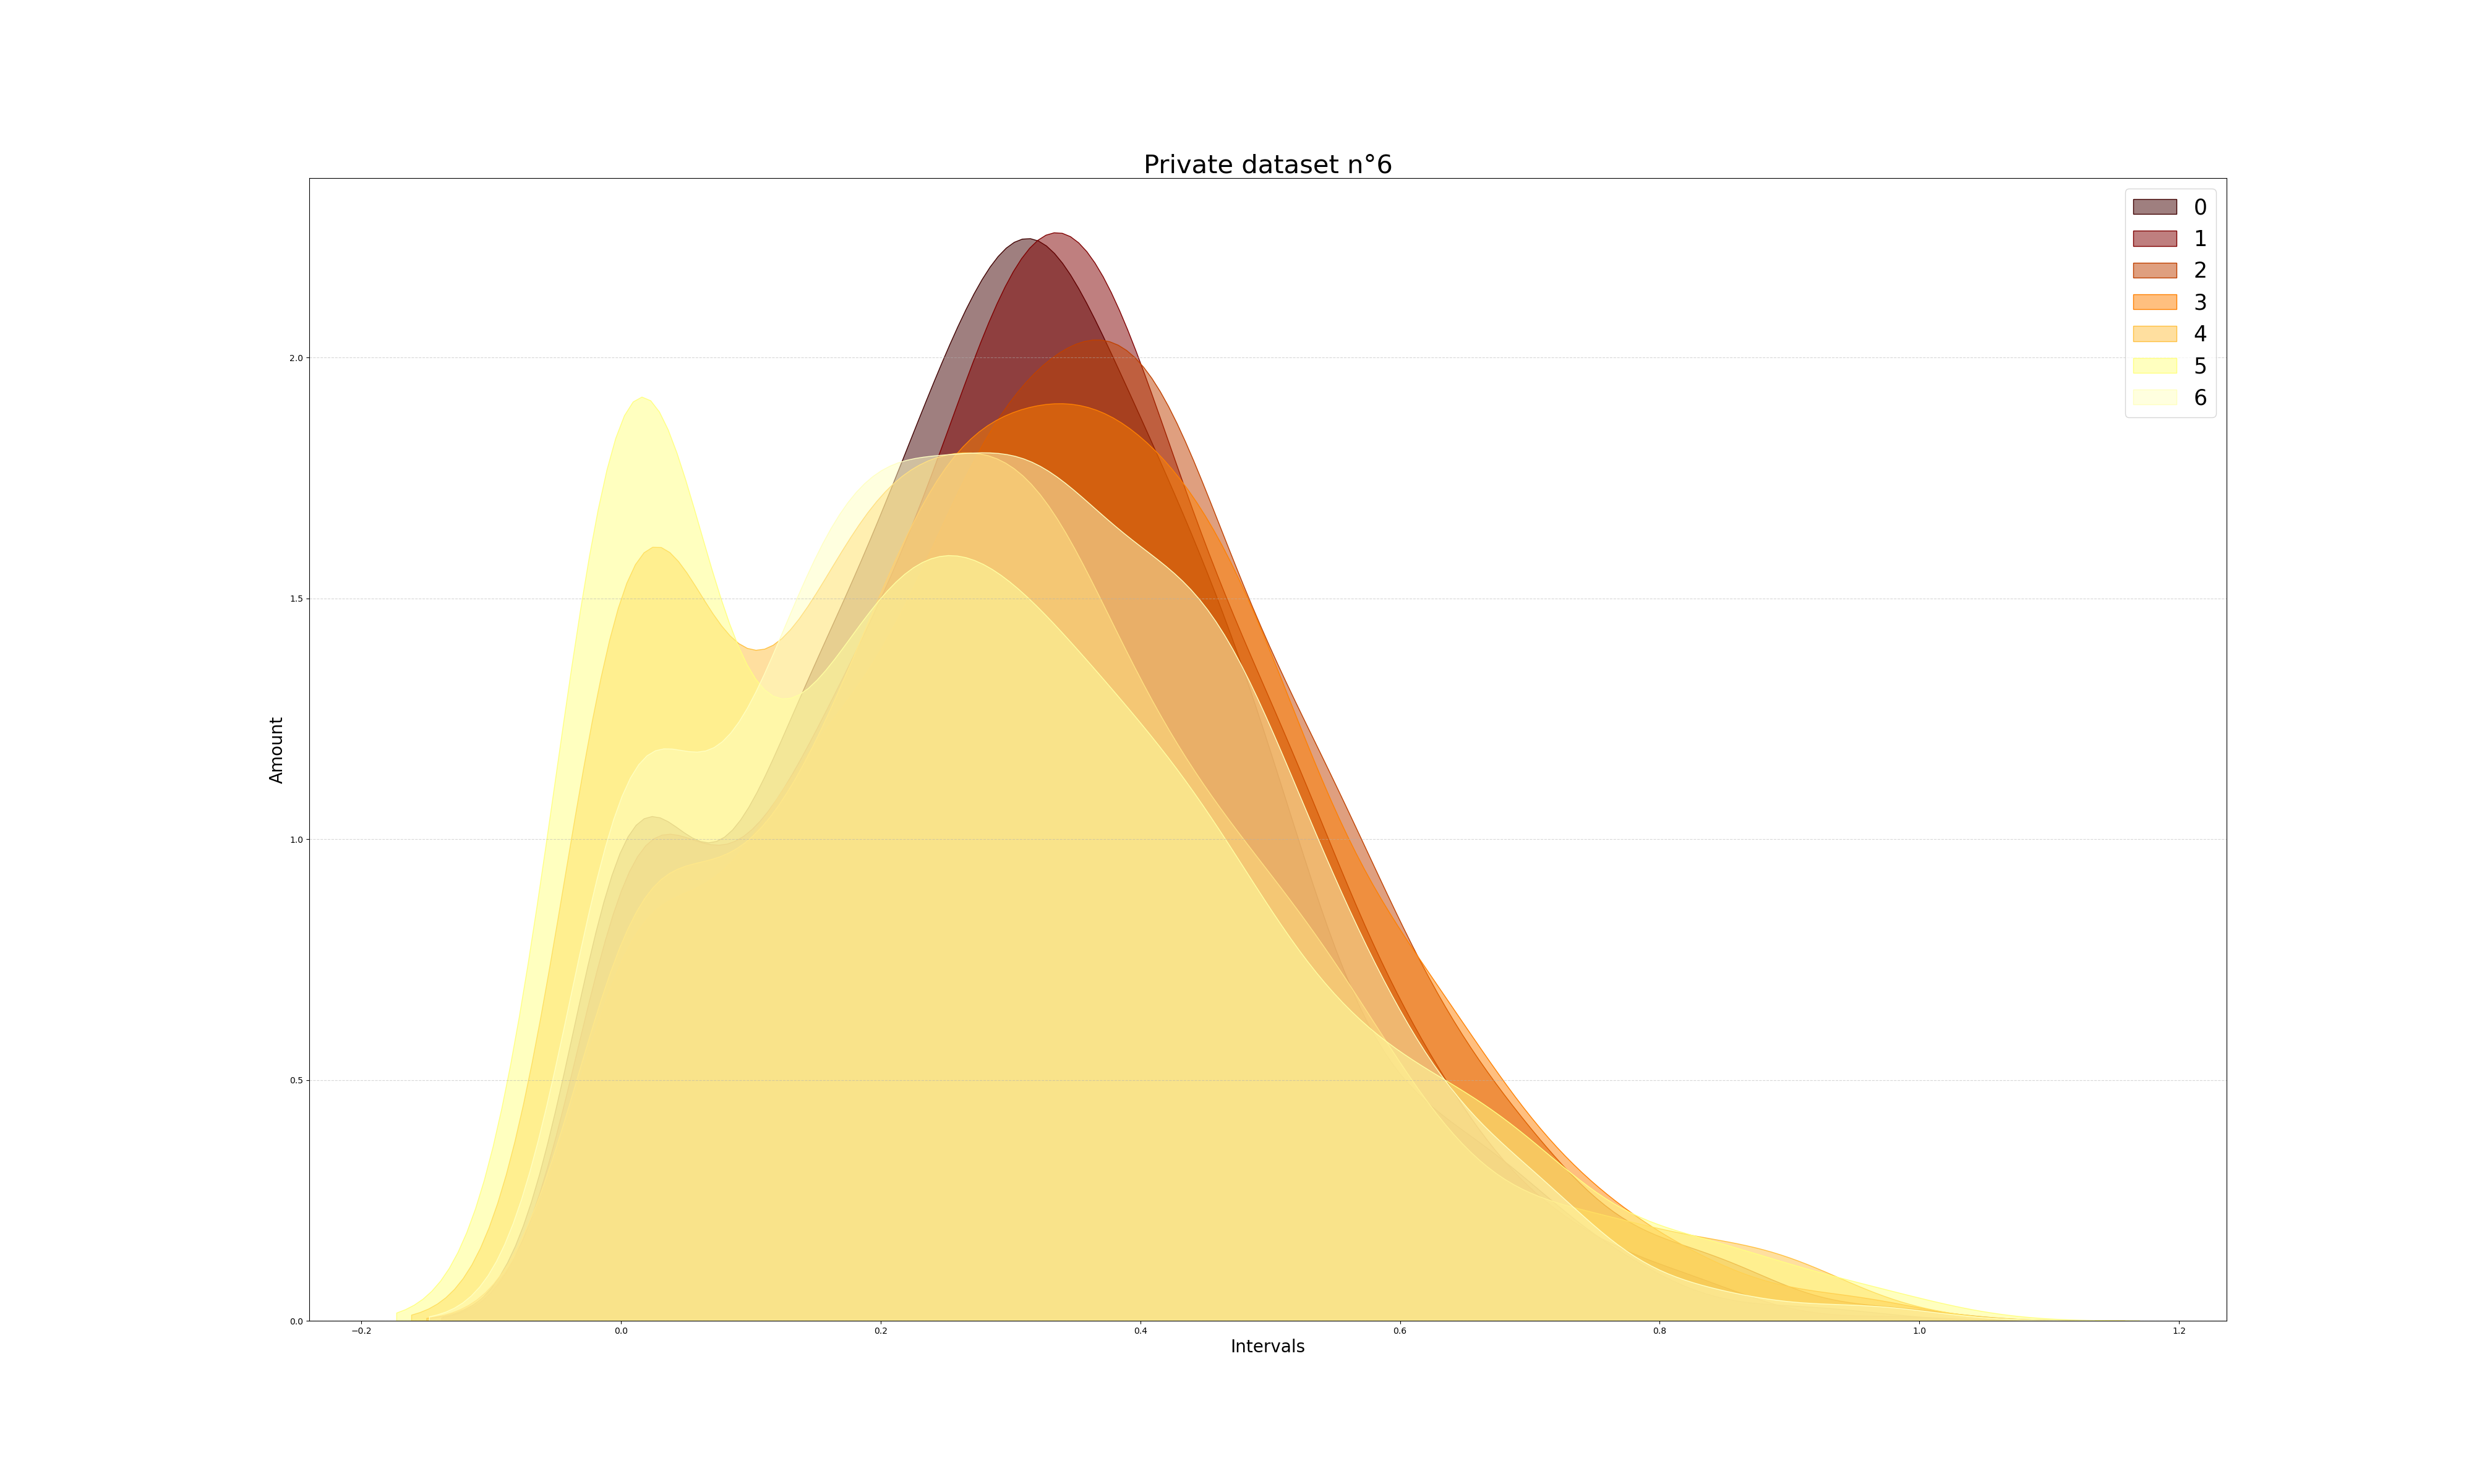
\includegraphics[width = 0.28\textwidth]{figures/Resultats/privateDS/Task 2/6}}}\qquad
            \subfloat[]{\fbox{
                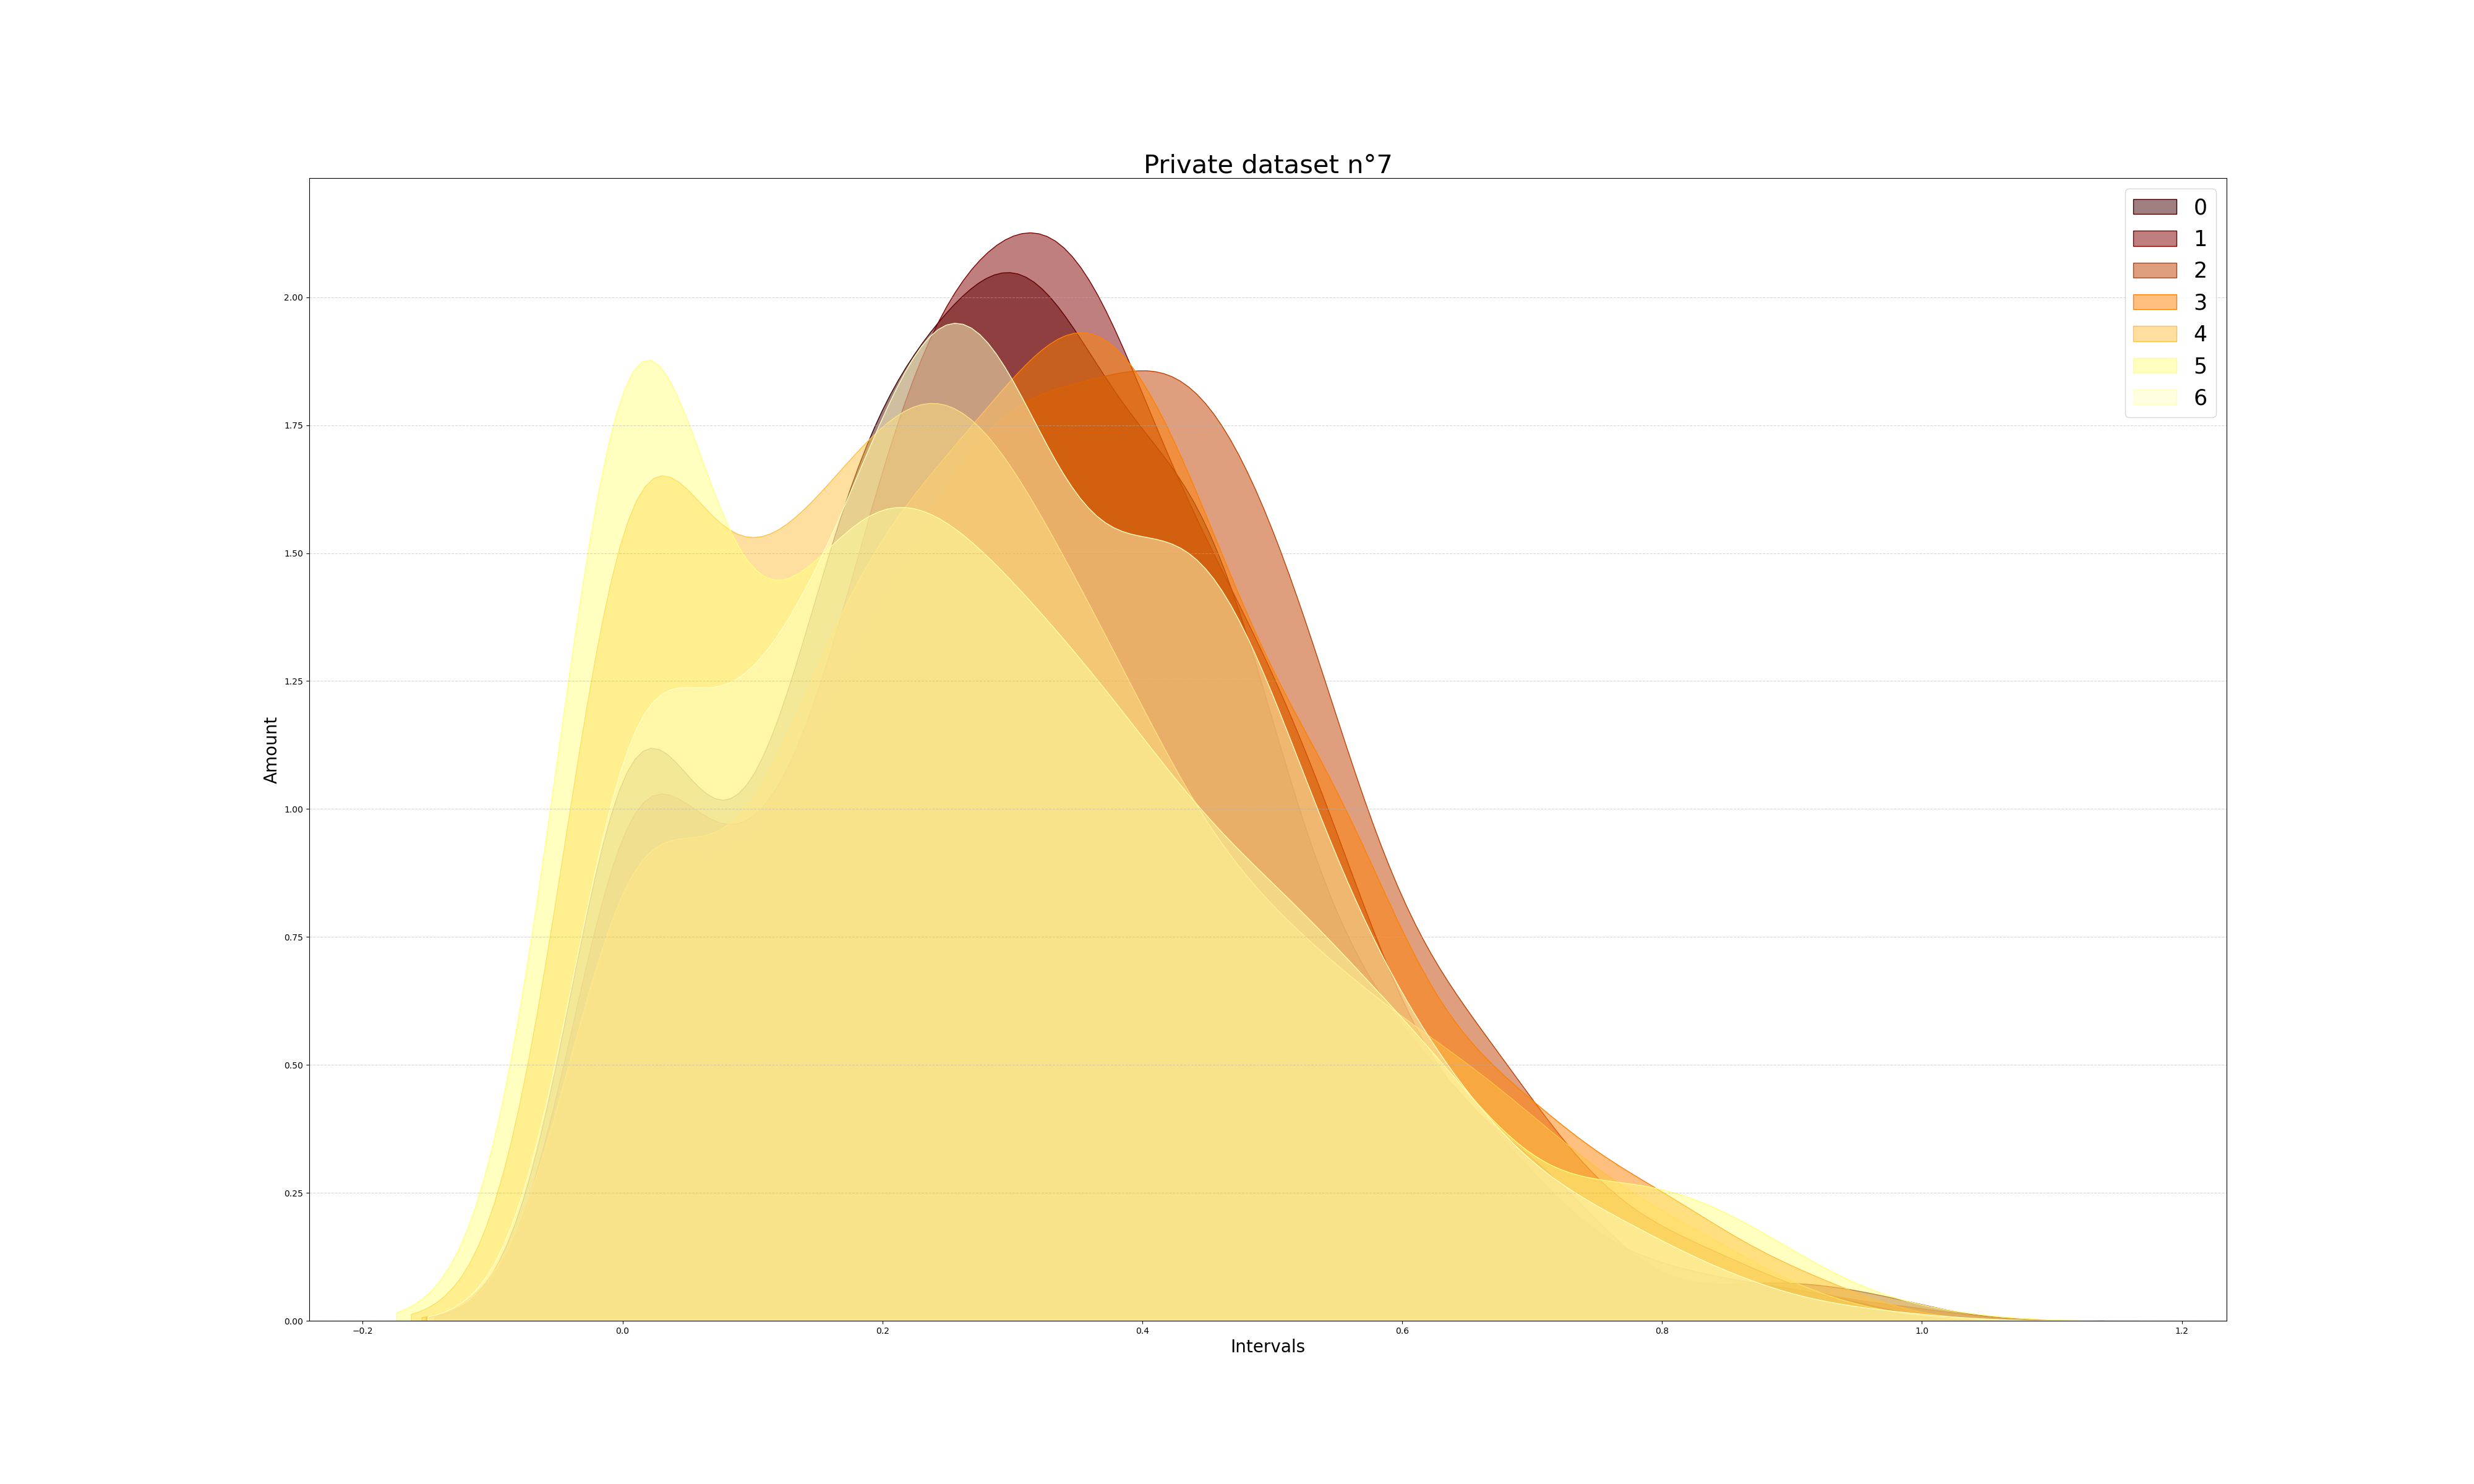
\includegraphics[width = 0.28\textwidth]{figures/Resultats/privateDS/Task 2/7}}}\qquad
            \subfloat[]{\fbox{
                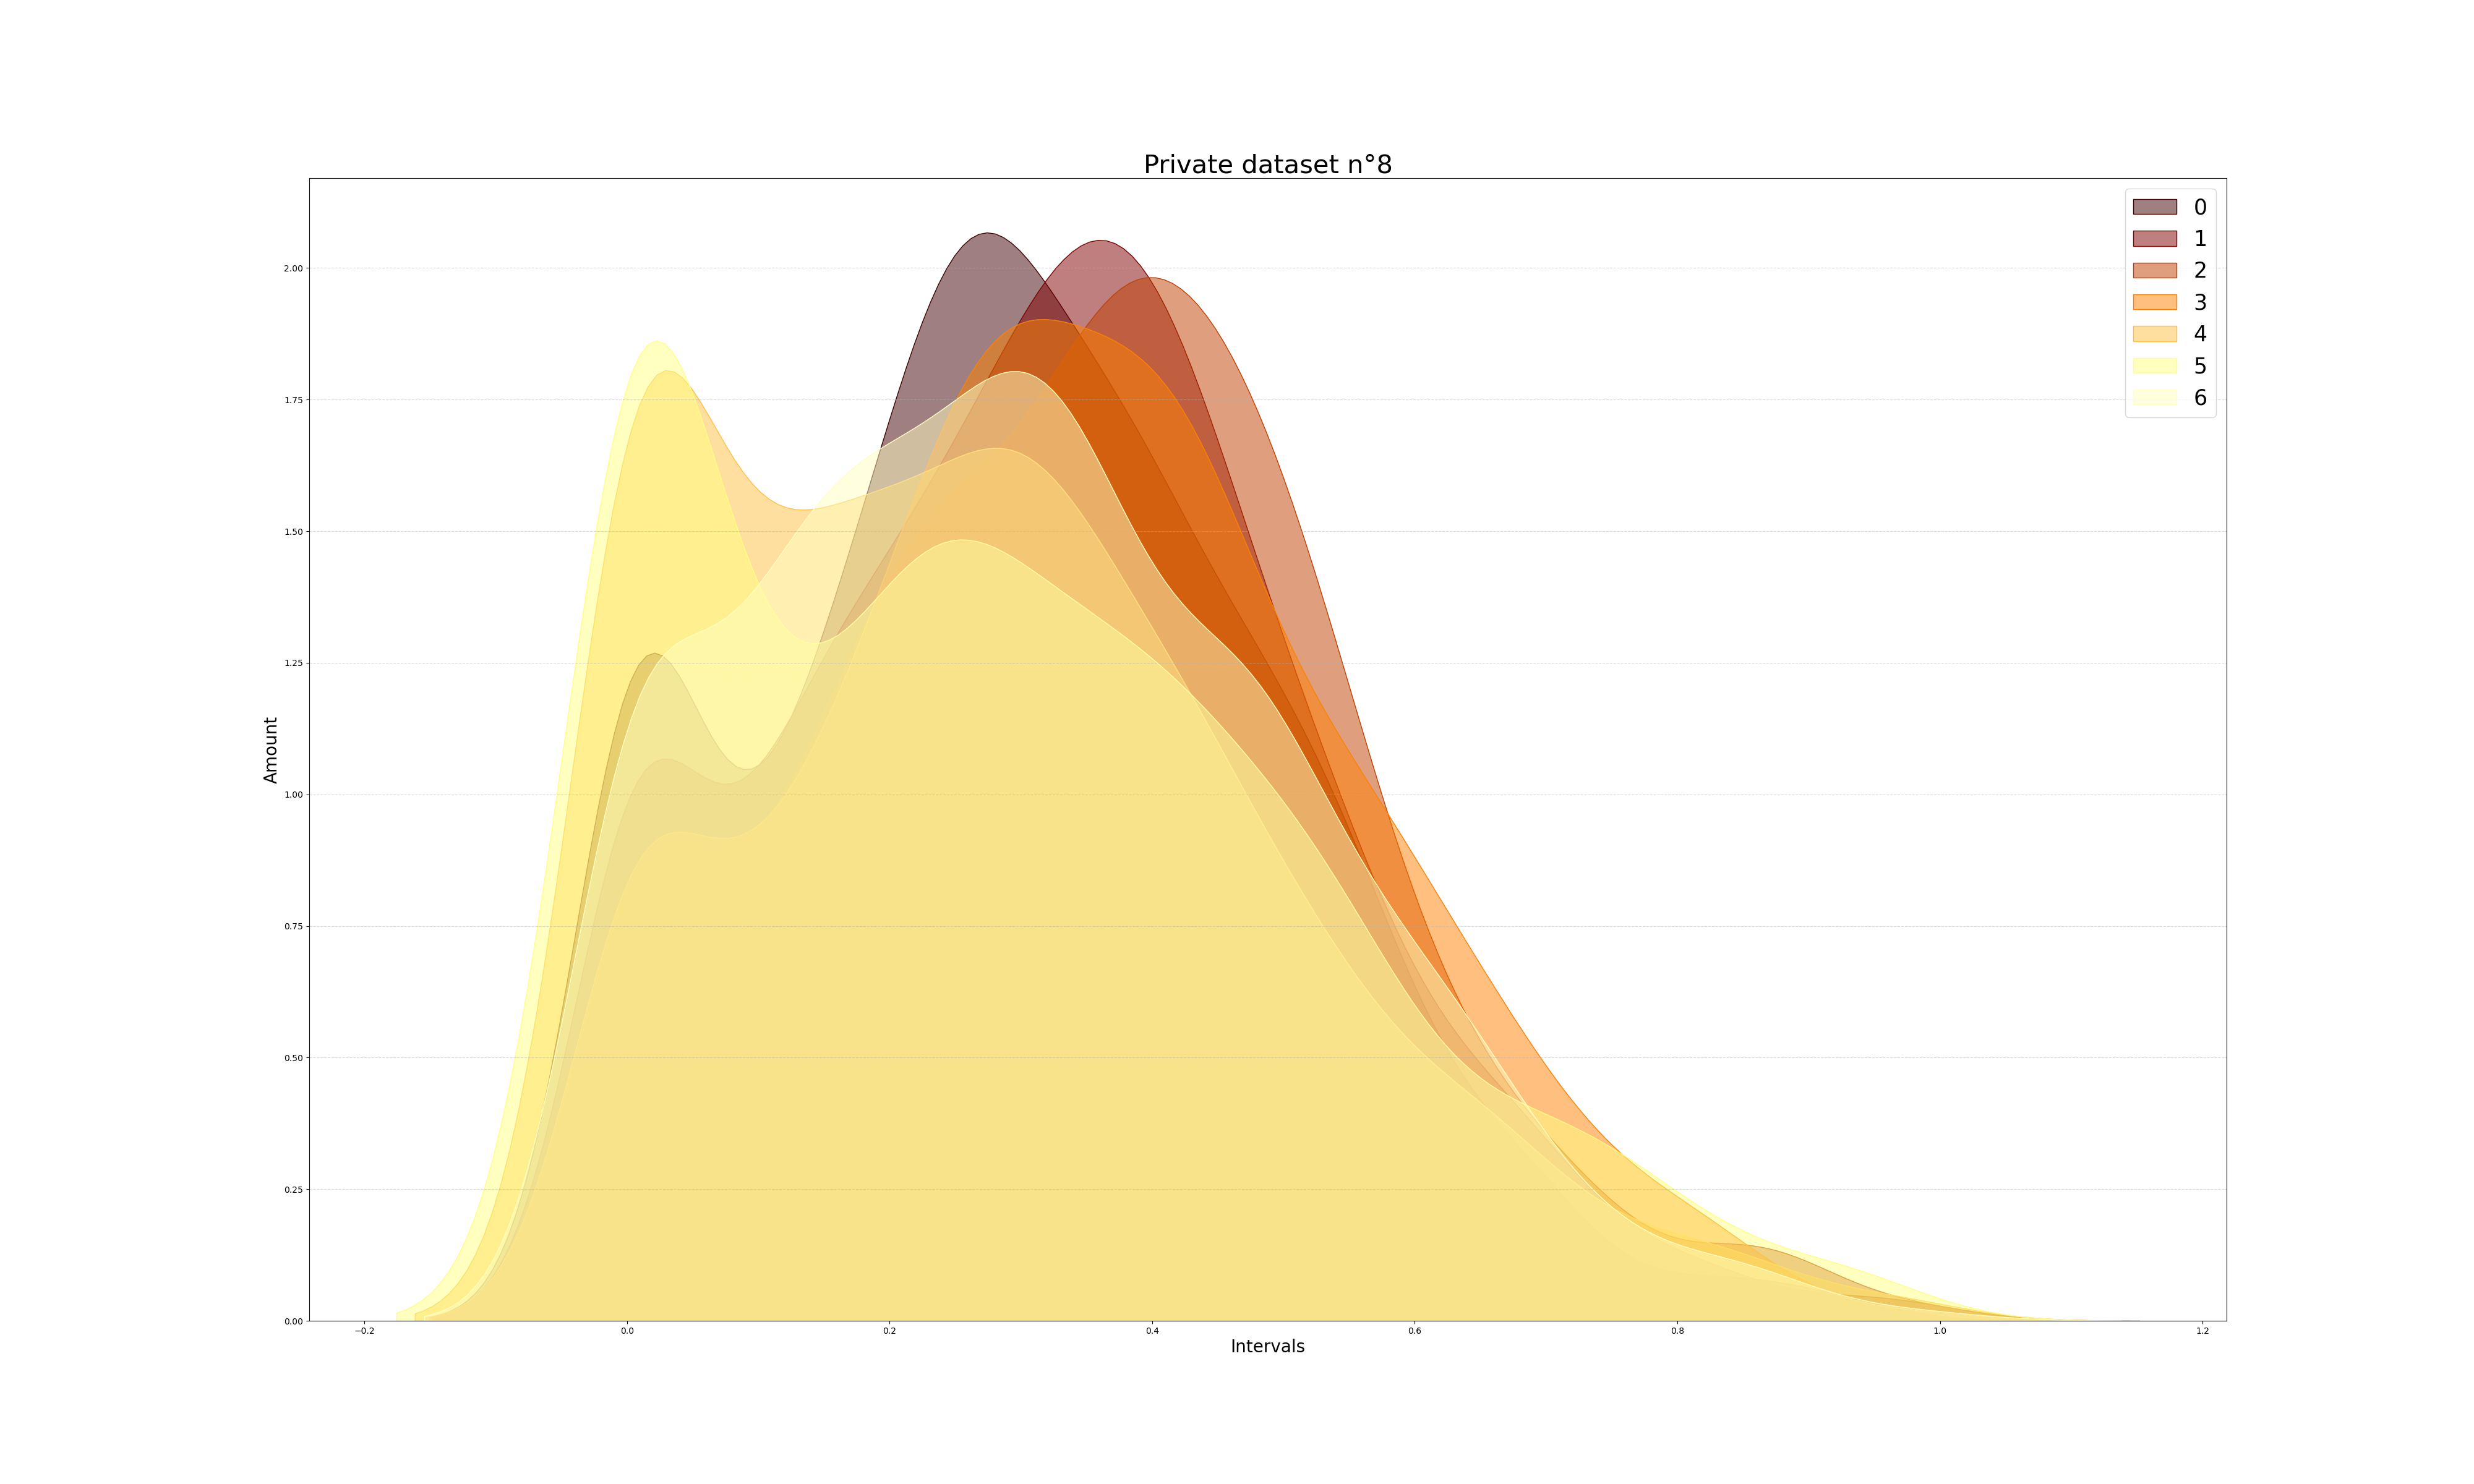
\includegraphics[width = 0.28\textwidth]{figures/Resultats/privateDS/Task 2/8}}}\qquad
            \subfloat[]{\fbox{
                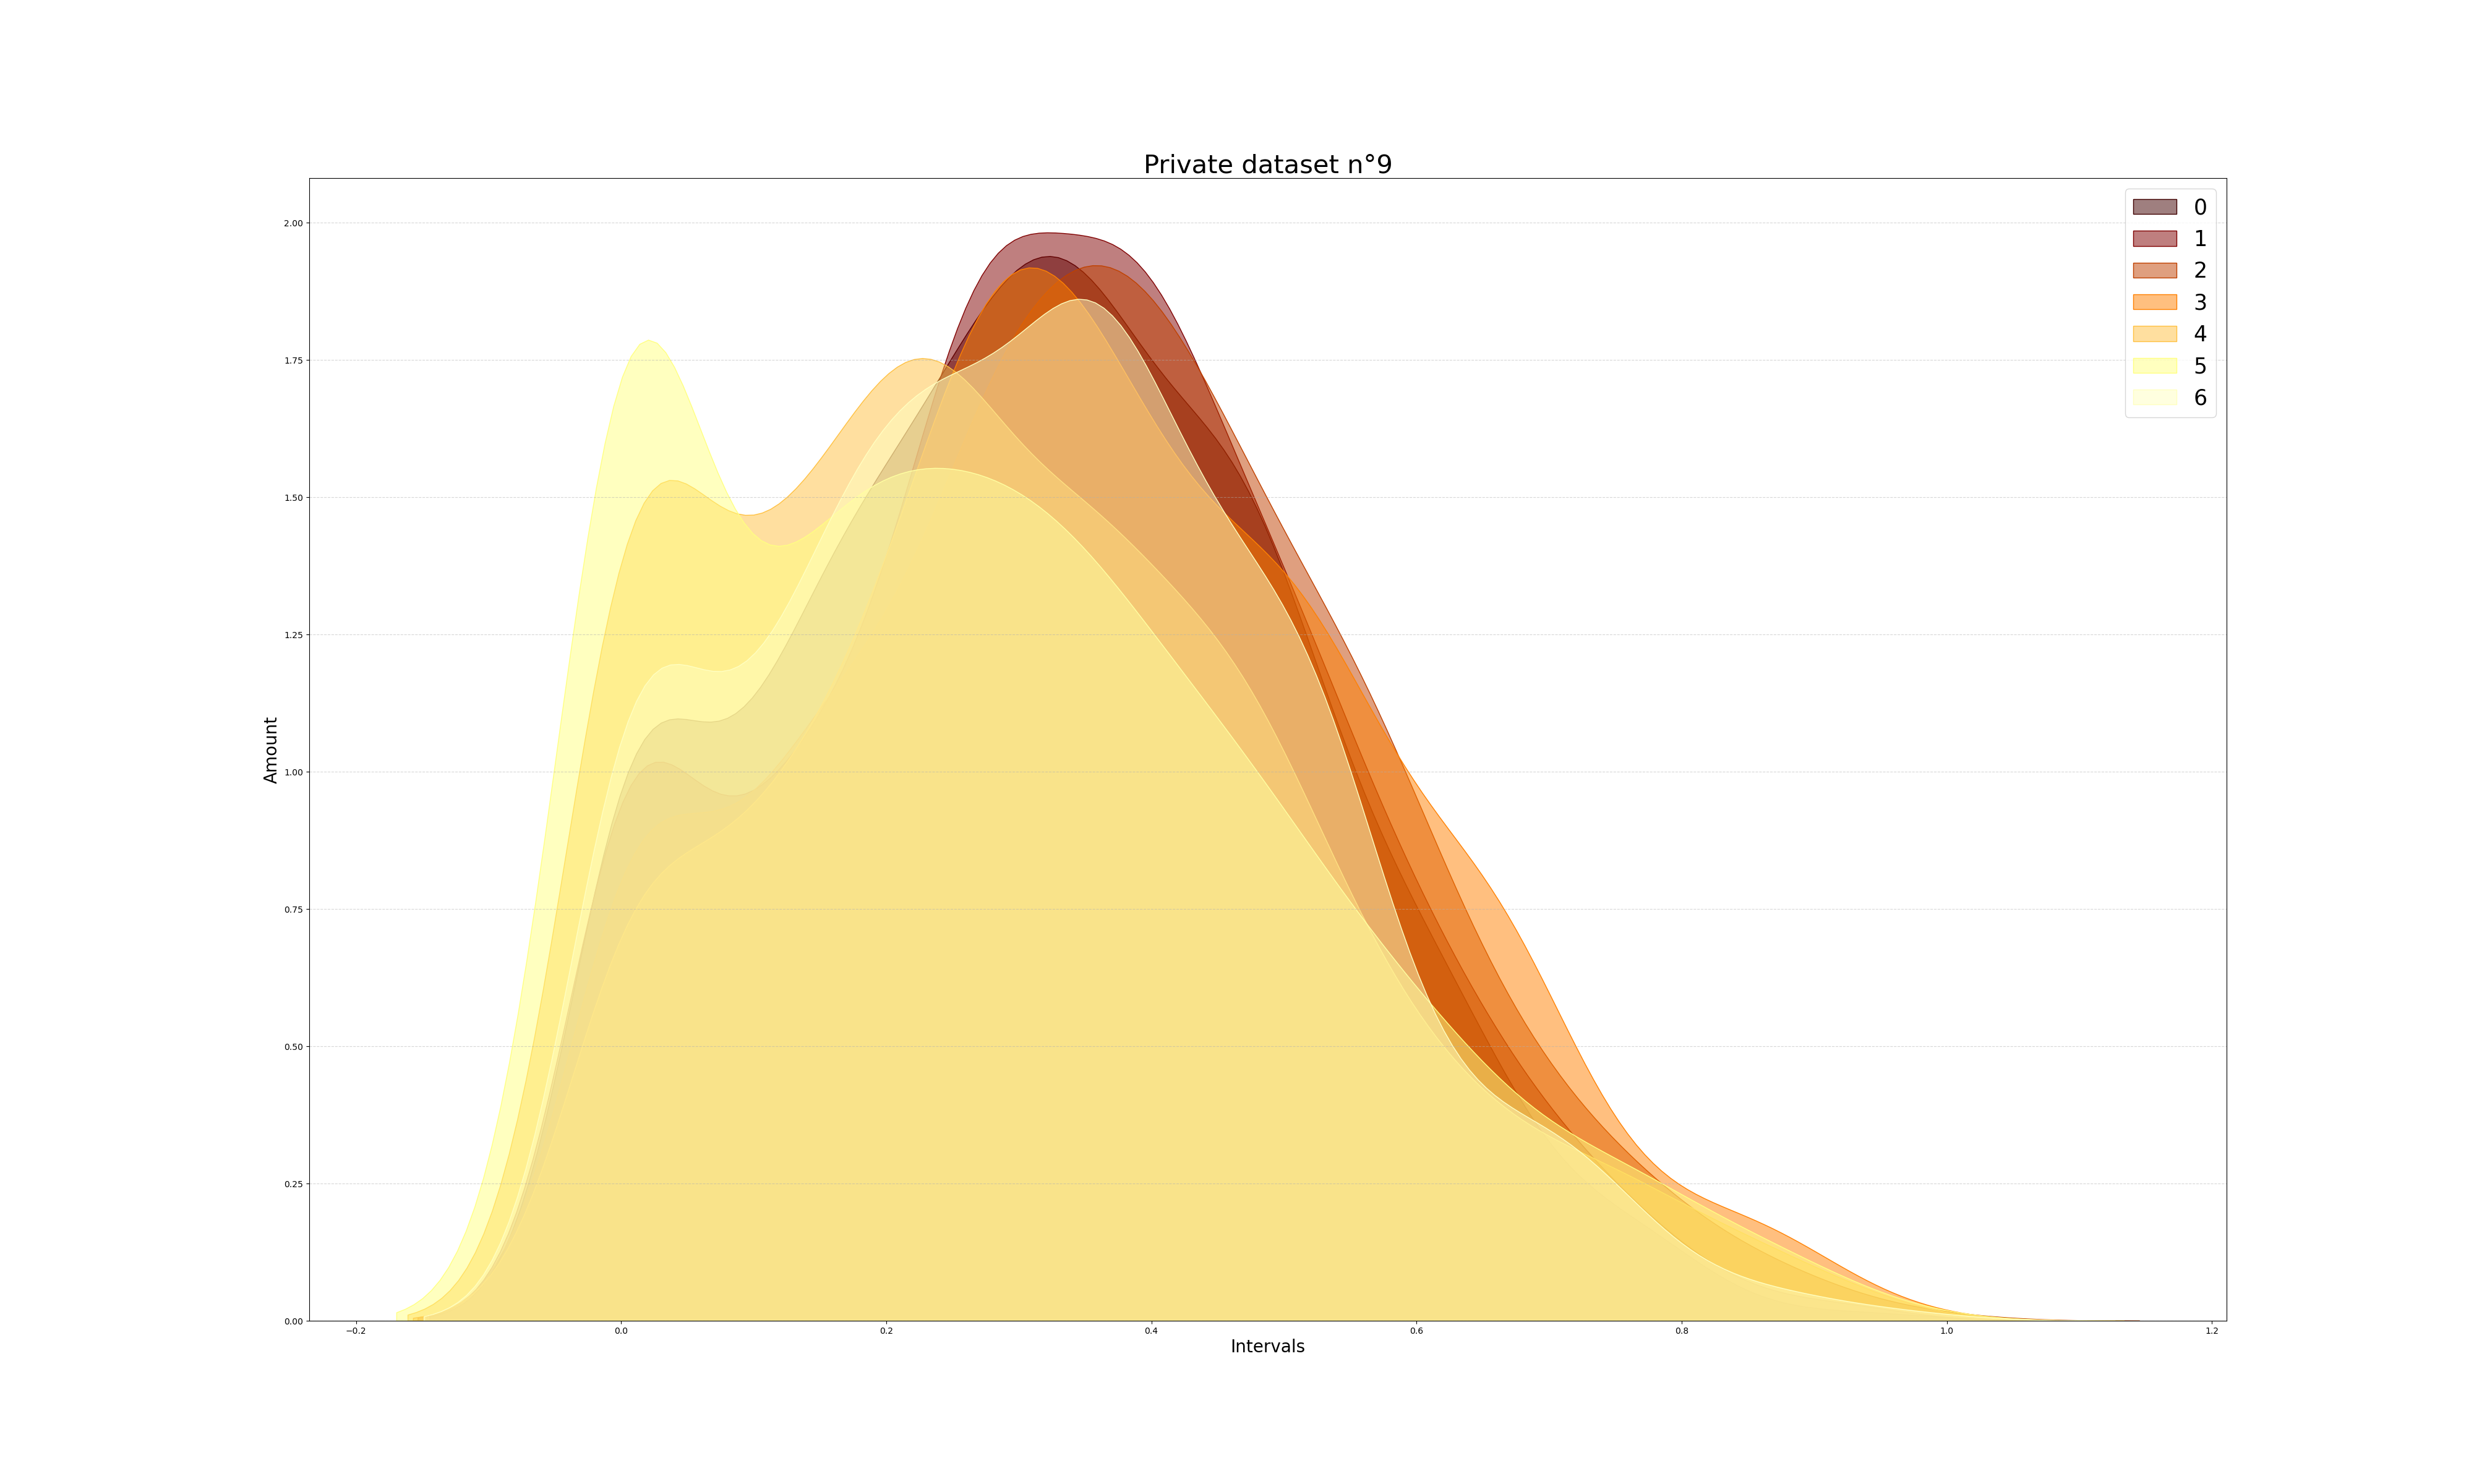
\includegraphics[width = 0.28\textwidth]{figures/Resultats/privateDS/Task 2/9}}}\qquad
            \subfloat[]{\fbox{
                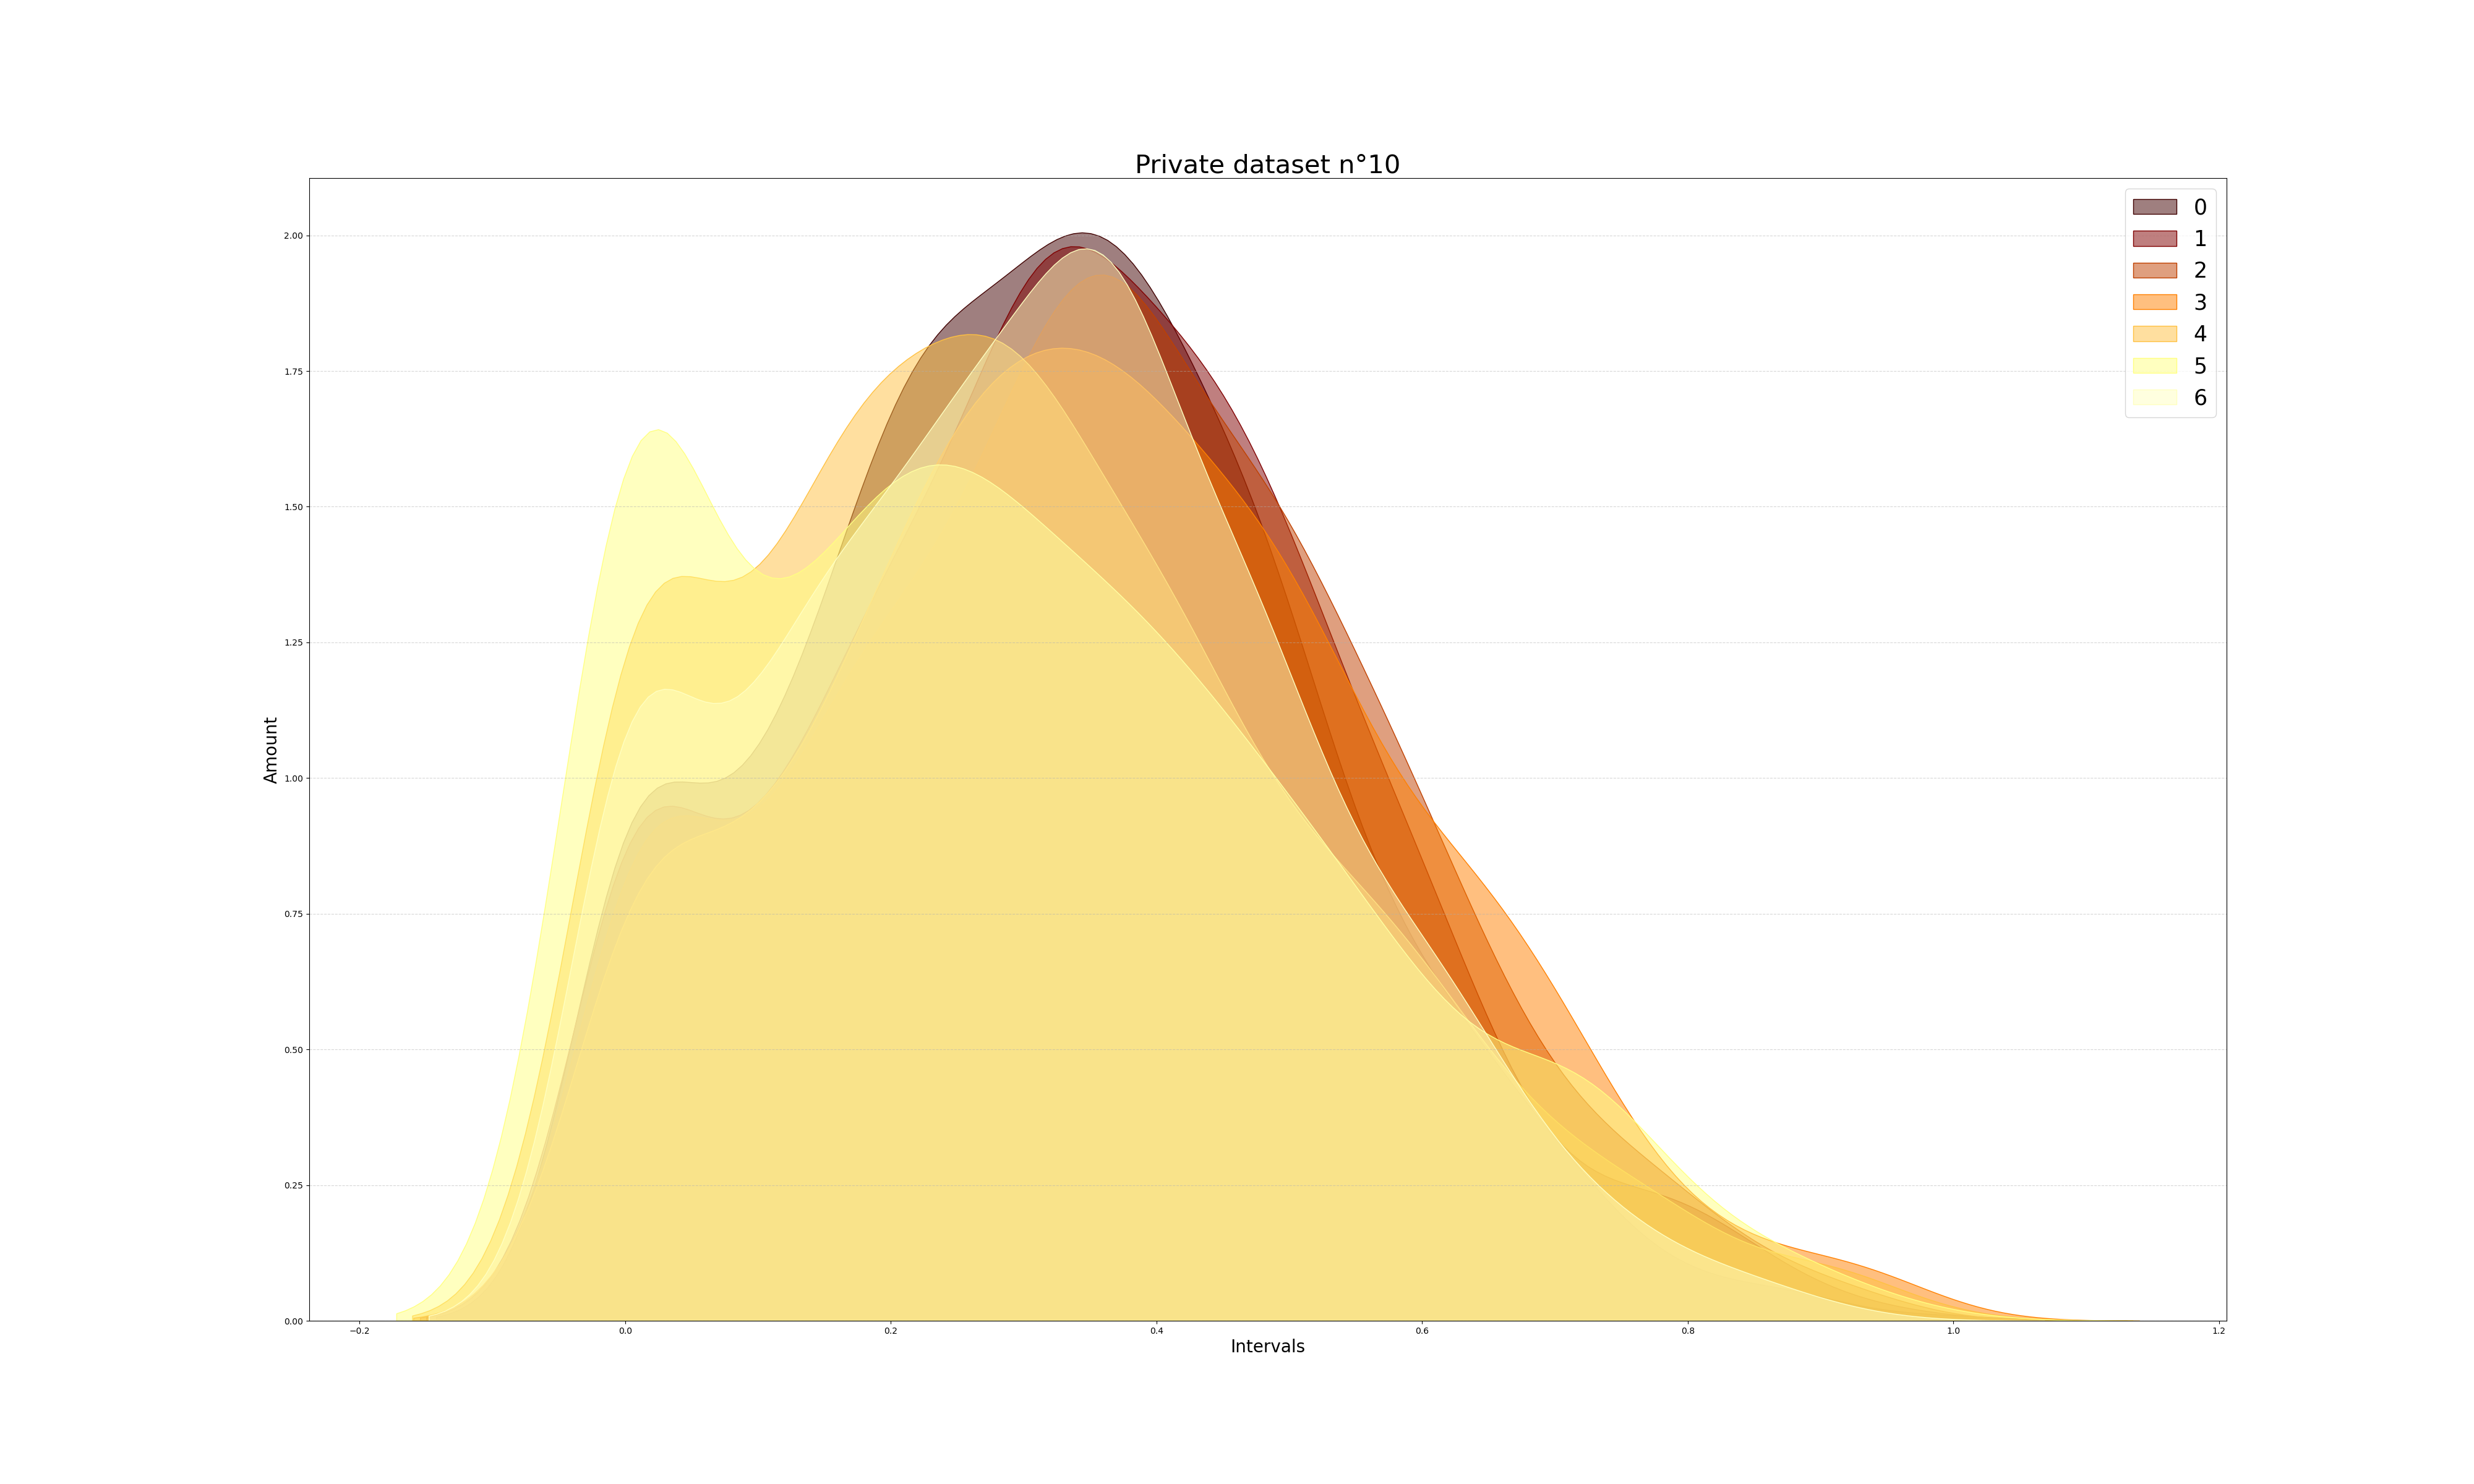
\includegraphics[width = 0.28\textwidth]{figures/Resultats/privateDS/Task 2/10}}}\qquad
            \subfloat[]{\fbox{
                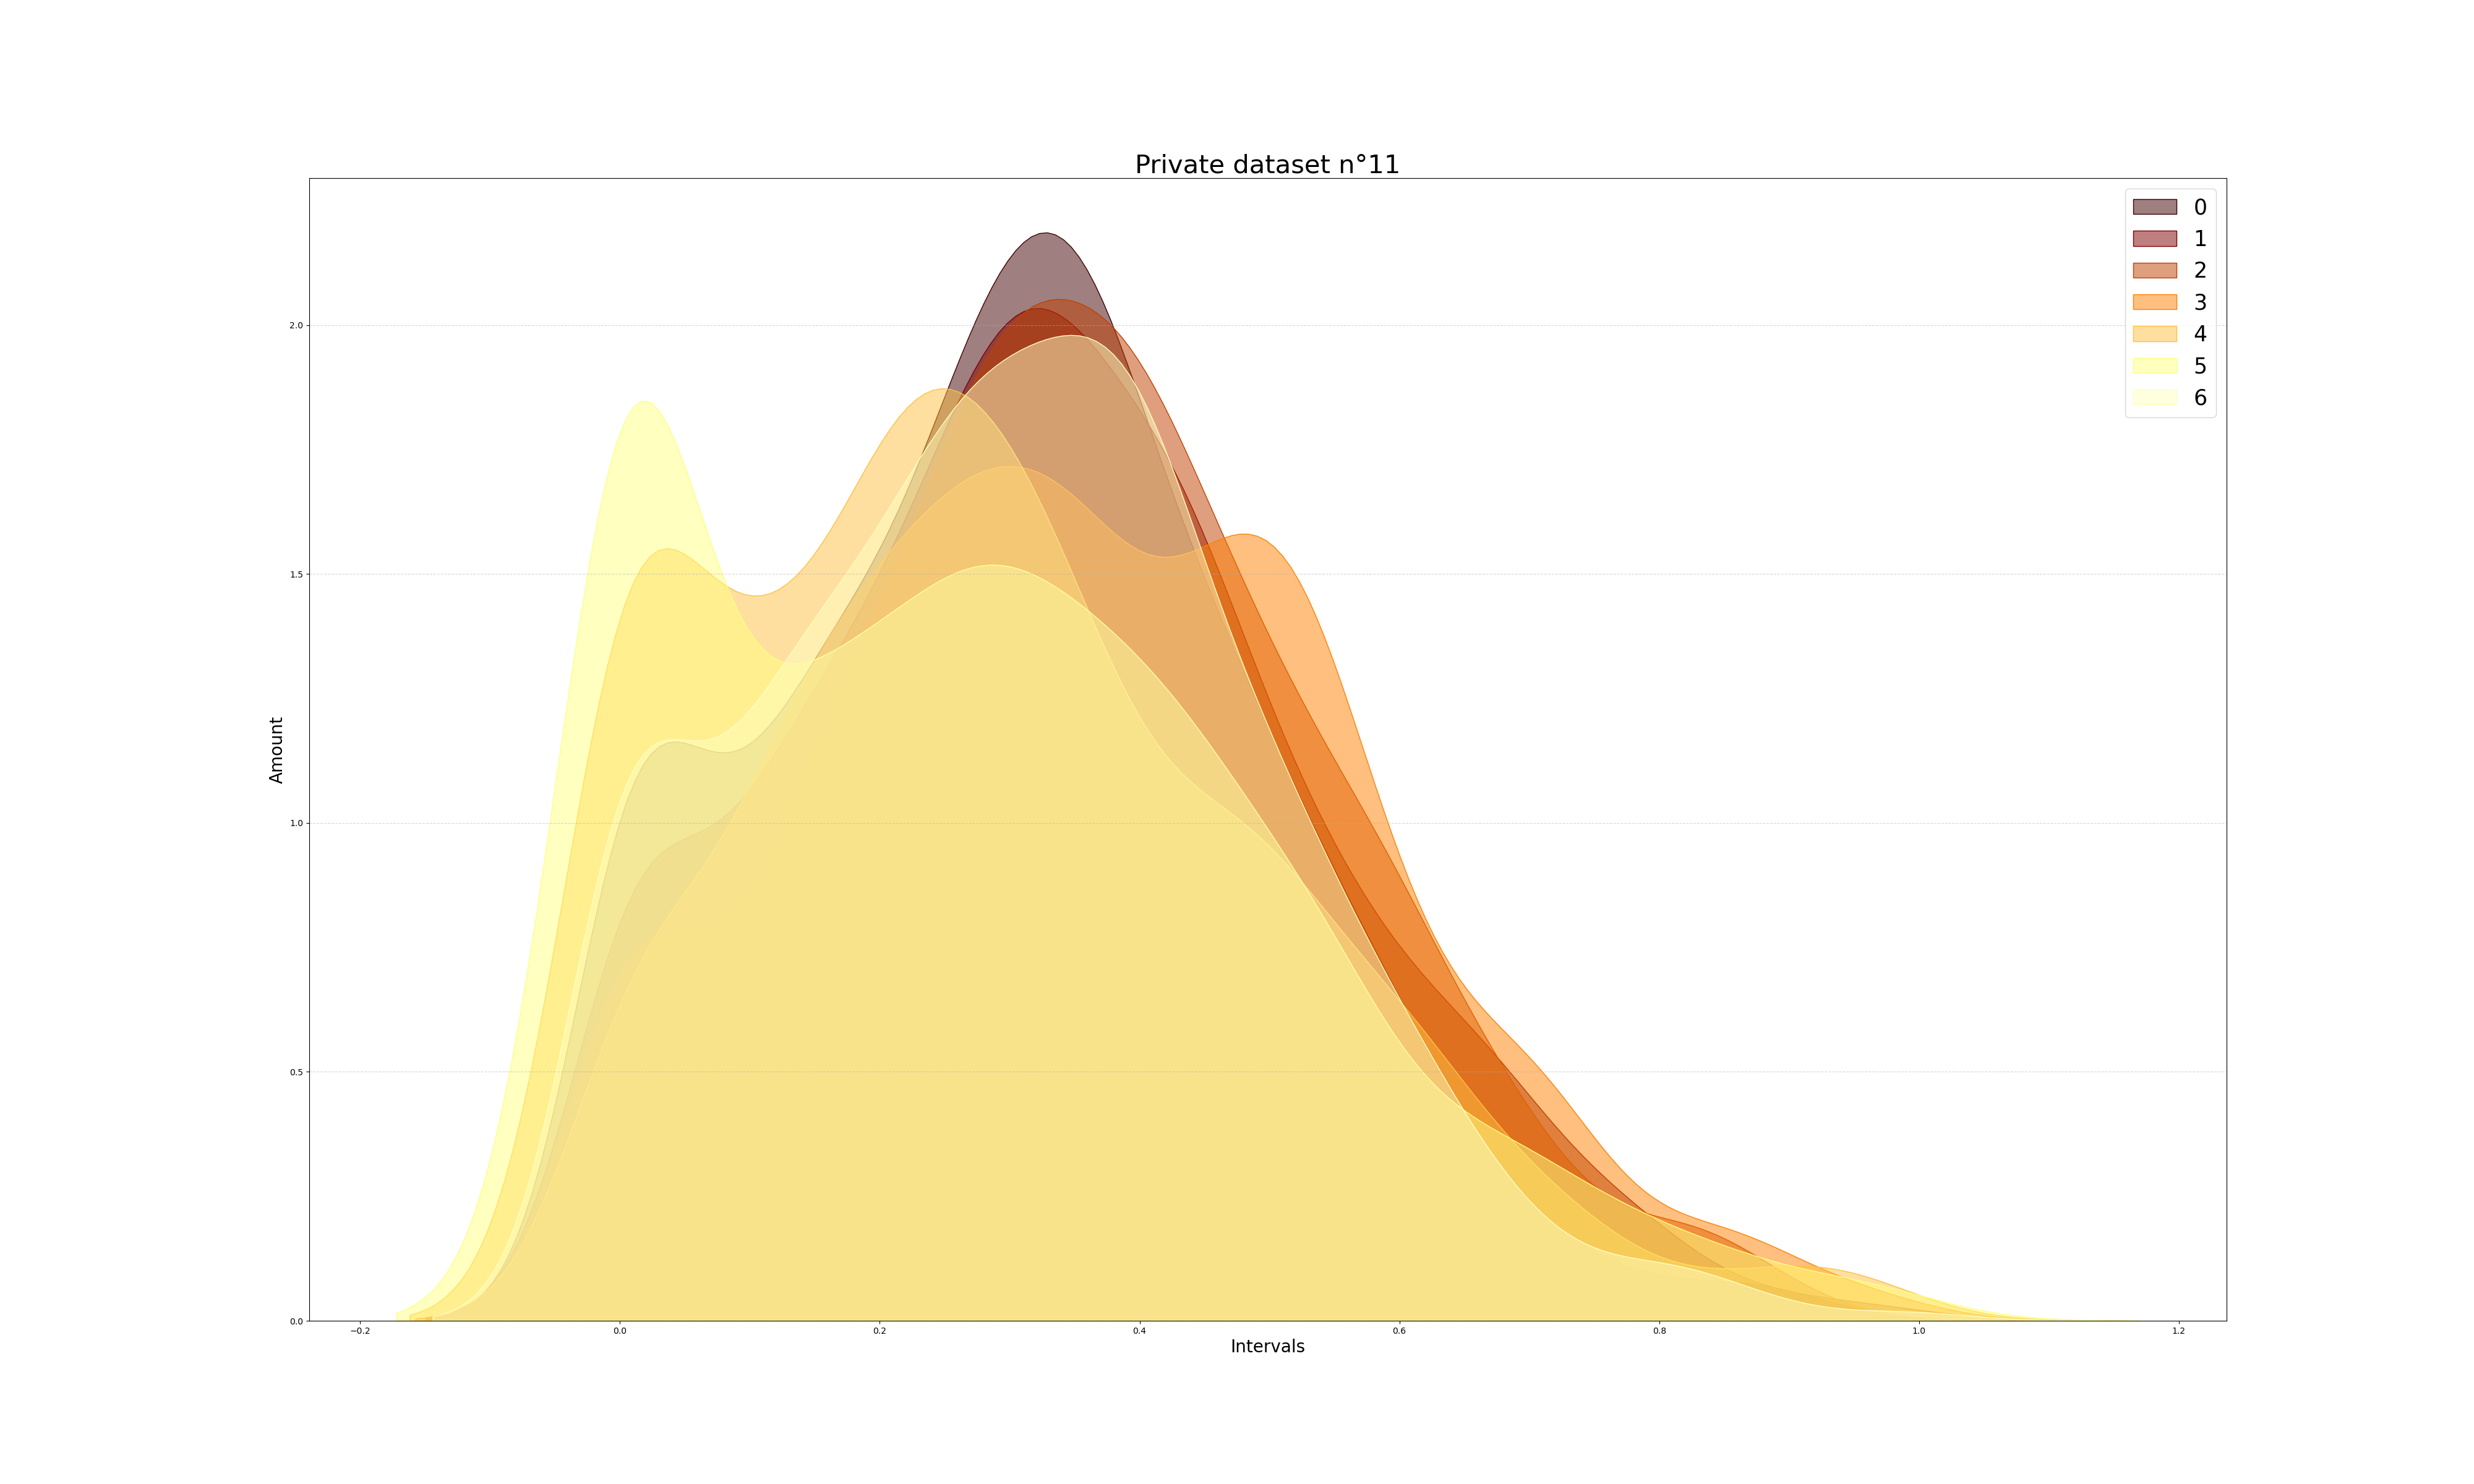
\includegraphics[width = 0.28\textwidth]{figures/Resultats/privateDS/Task 2/11}}}\qquad
            \subfloat[]{\fbox{
                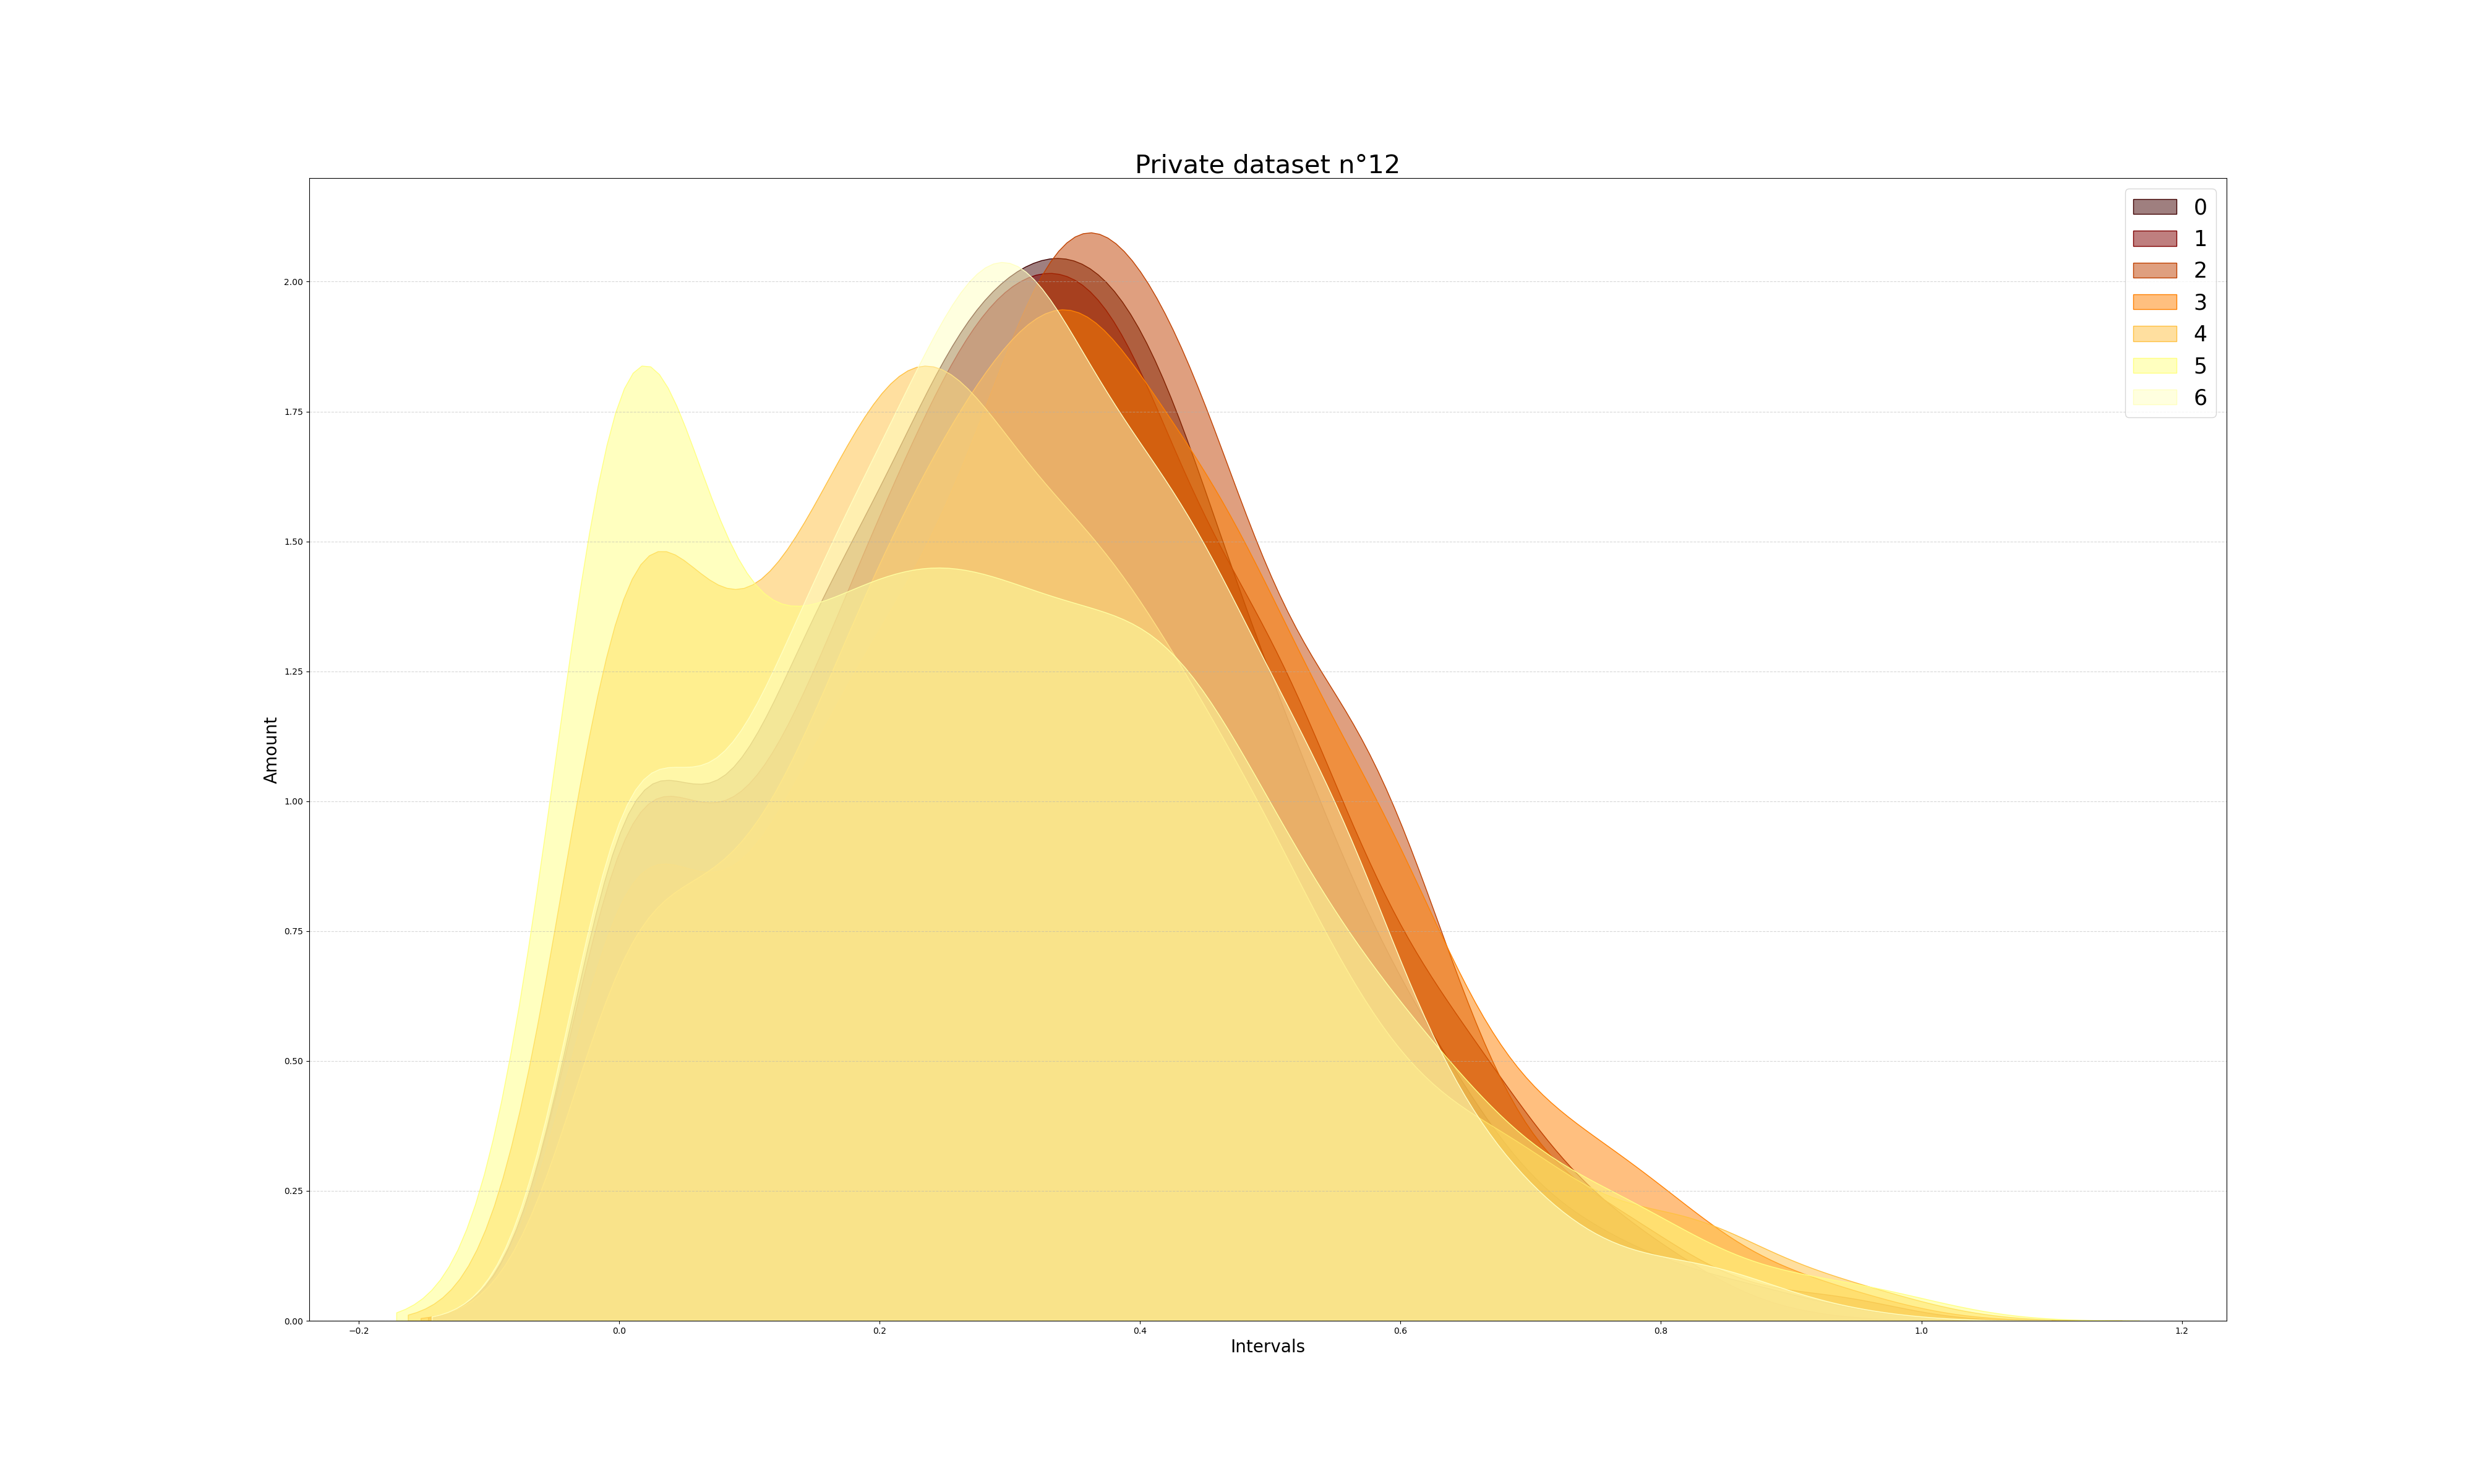
\includegraphics[width = 0.28\textwidth]{figures/Resultats/privateDS/Task 2/12}}}\qquad
            \subfloat[]{\fbox{
                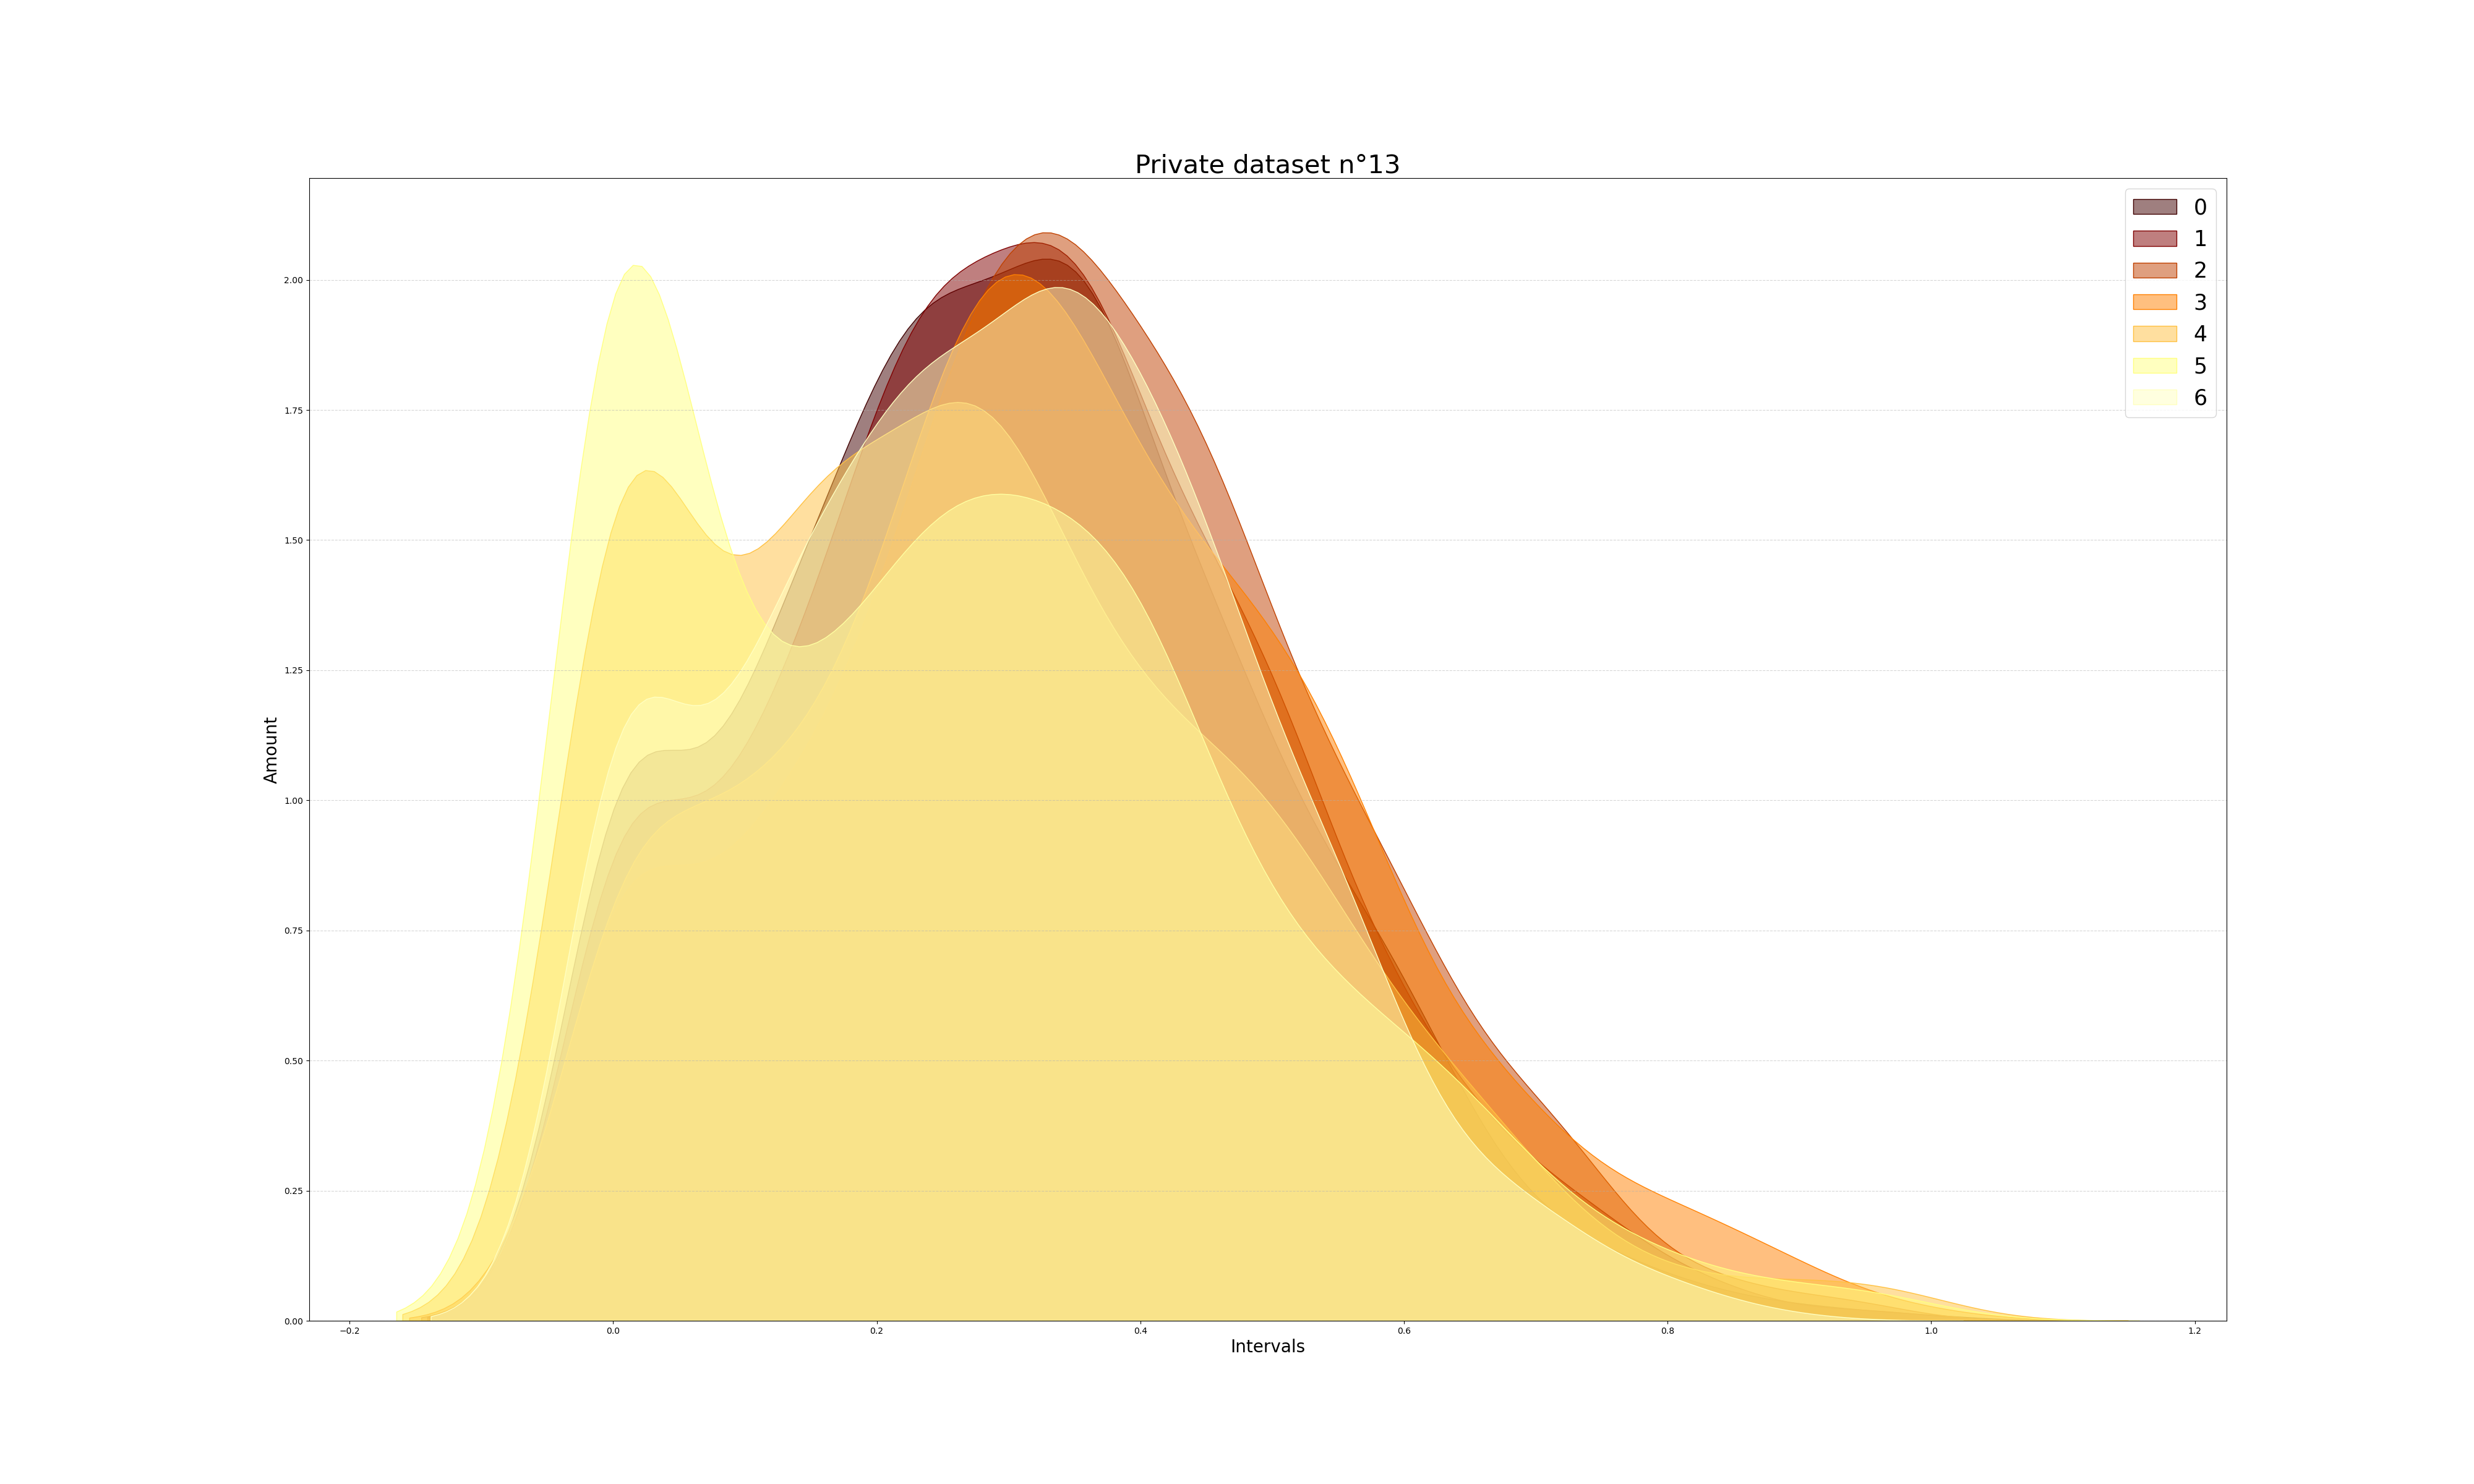
\includegraphics[width = 0.28\textwidth]{figures/Resultats/privateDS/Task 2/13}}}\qquad
            \subfloat[]{\fbox{
                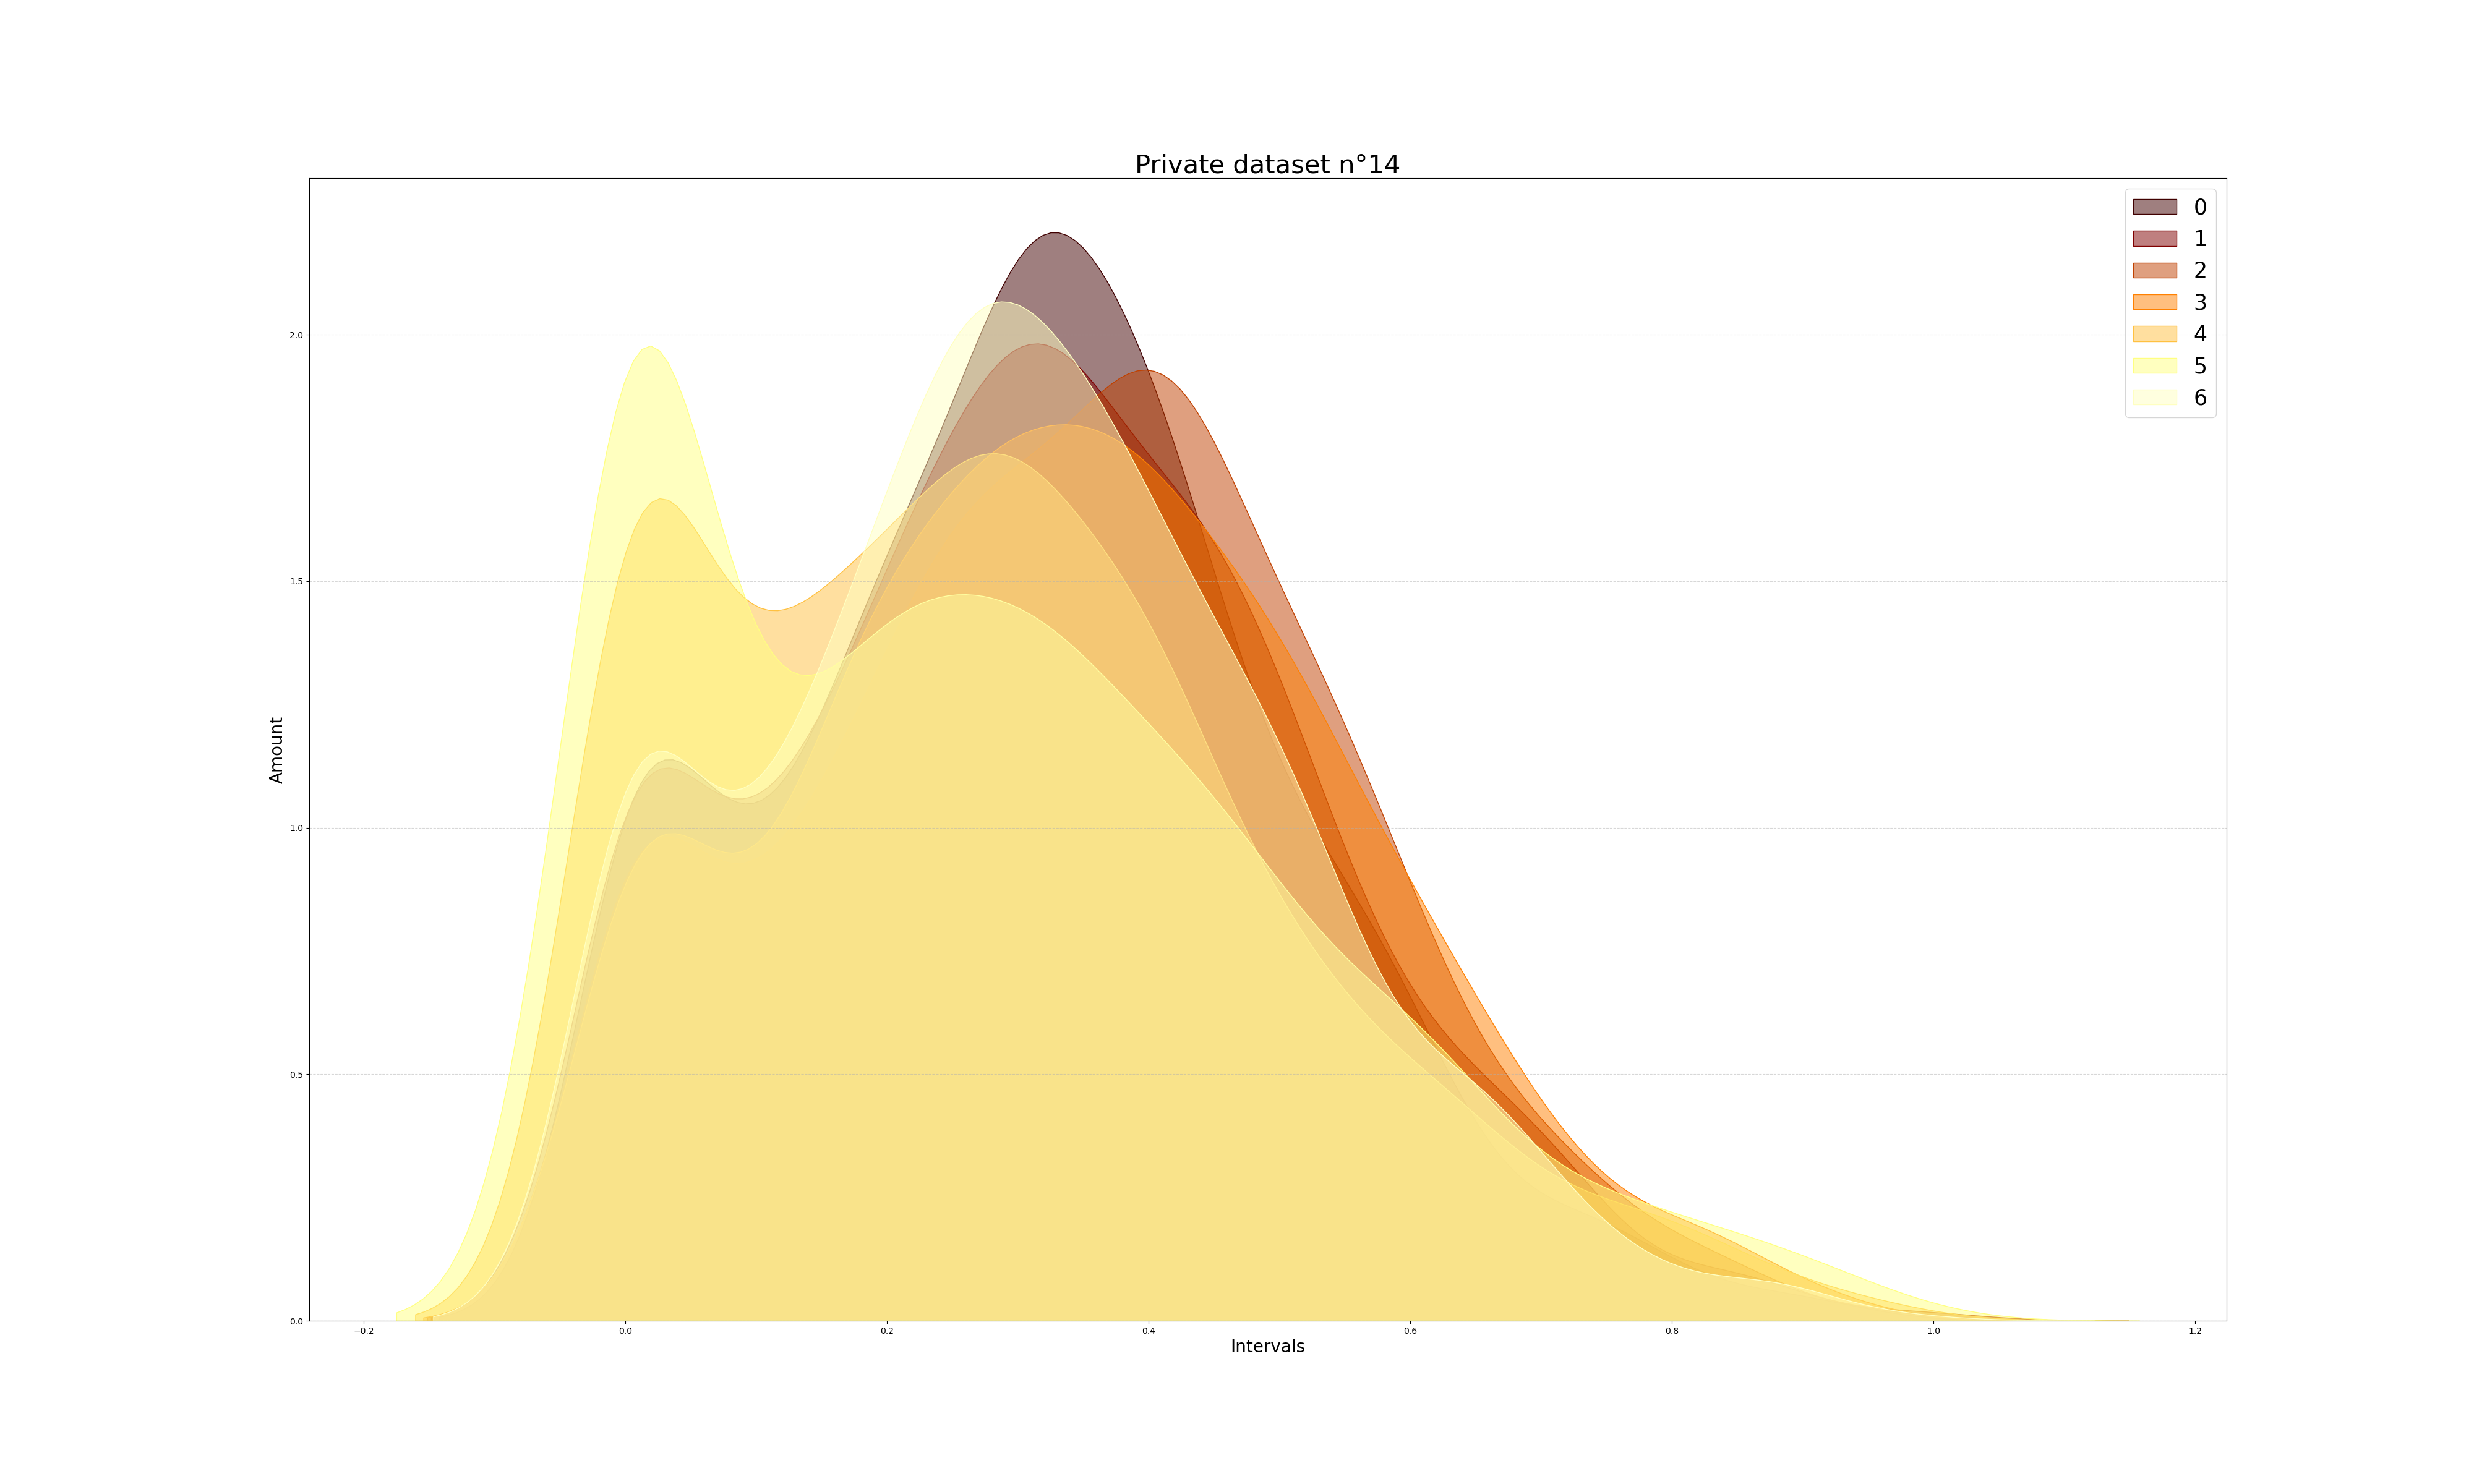
\includegraphics[width = 0.28\textwidth]{figures/Resultats/privateDS/Task 2/14}}}\qquad
            \subfloat[]{\fbox{
                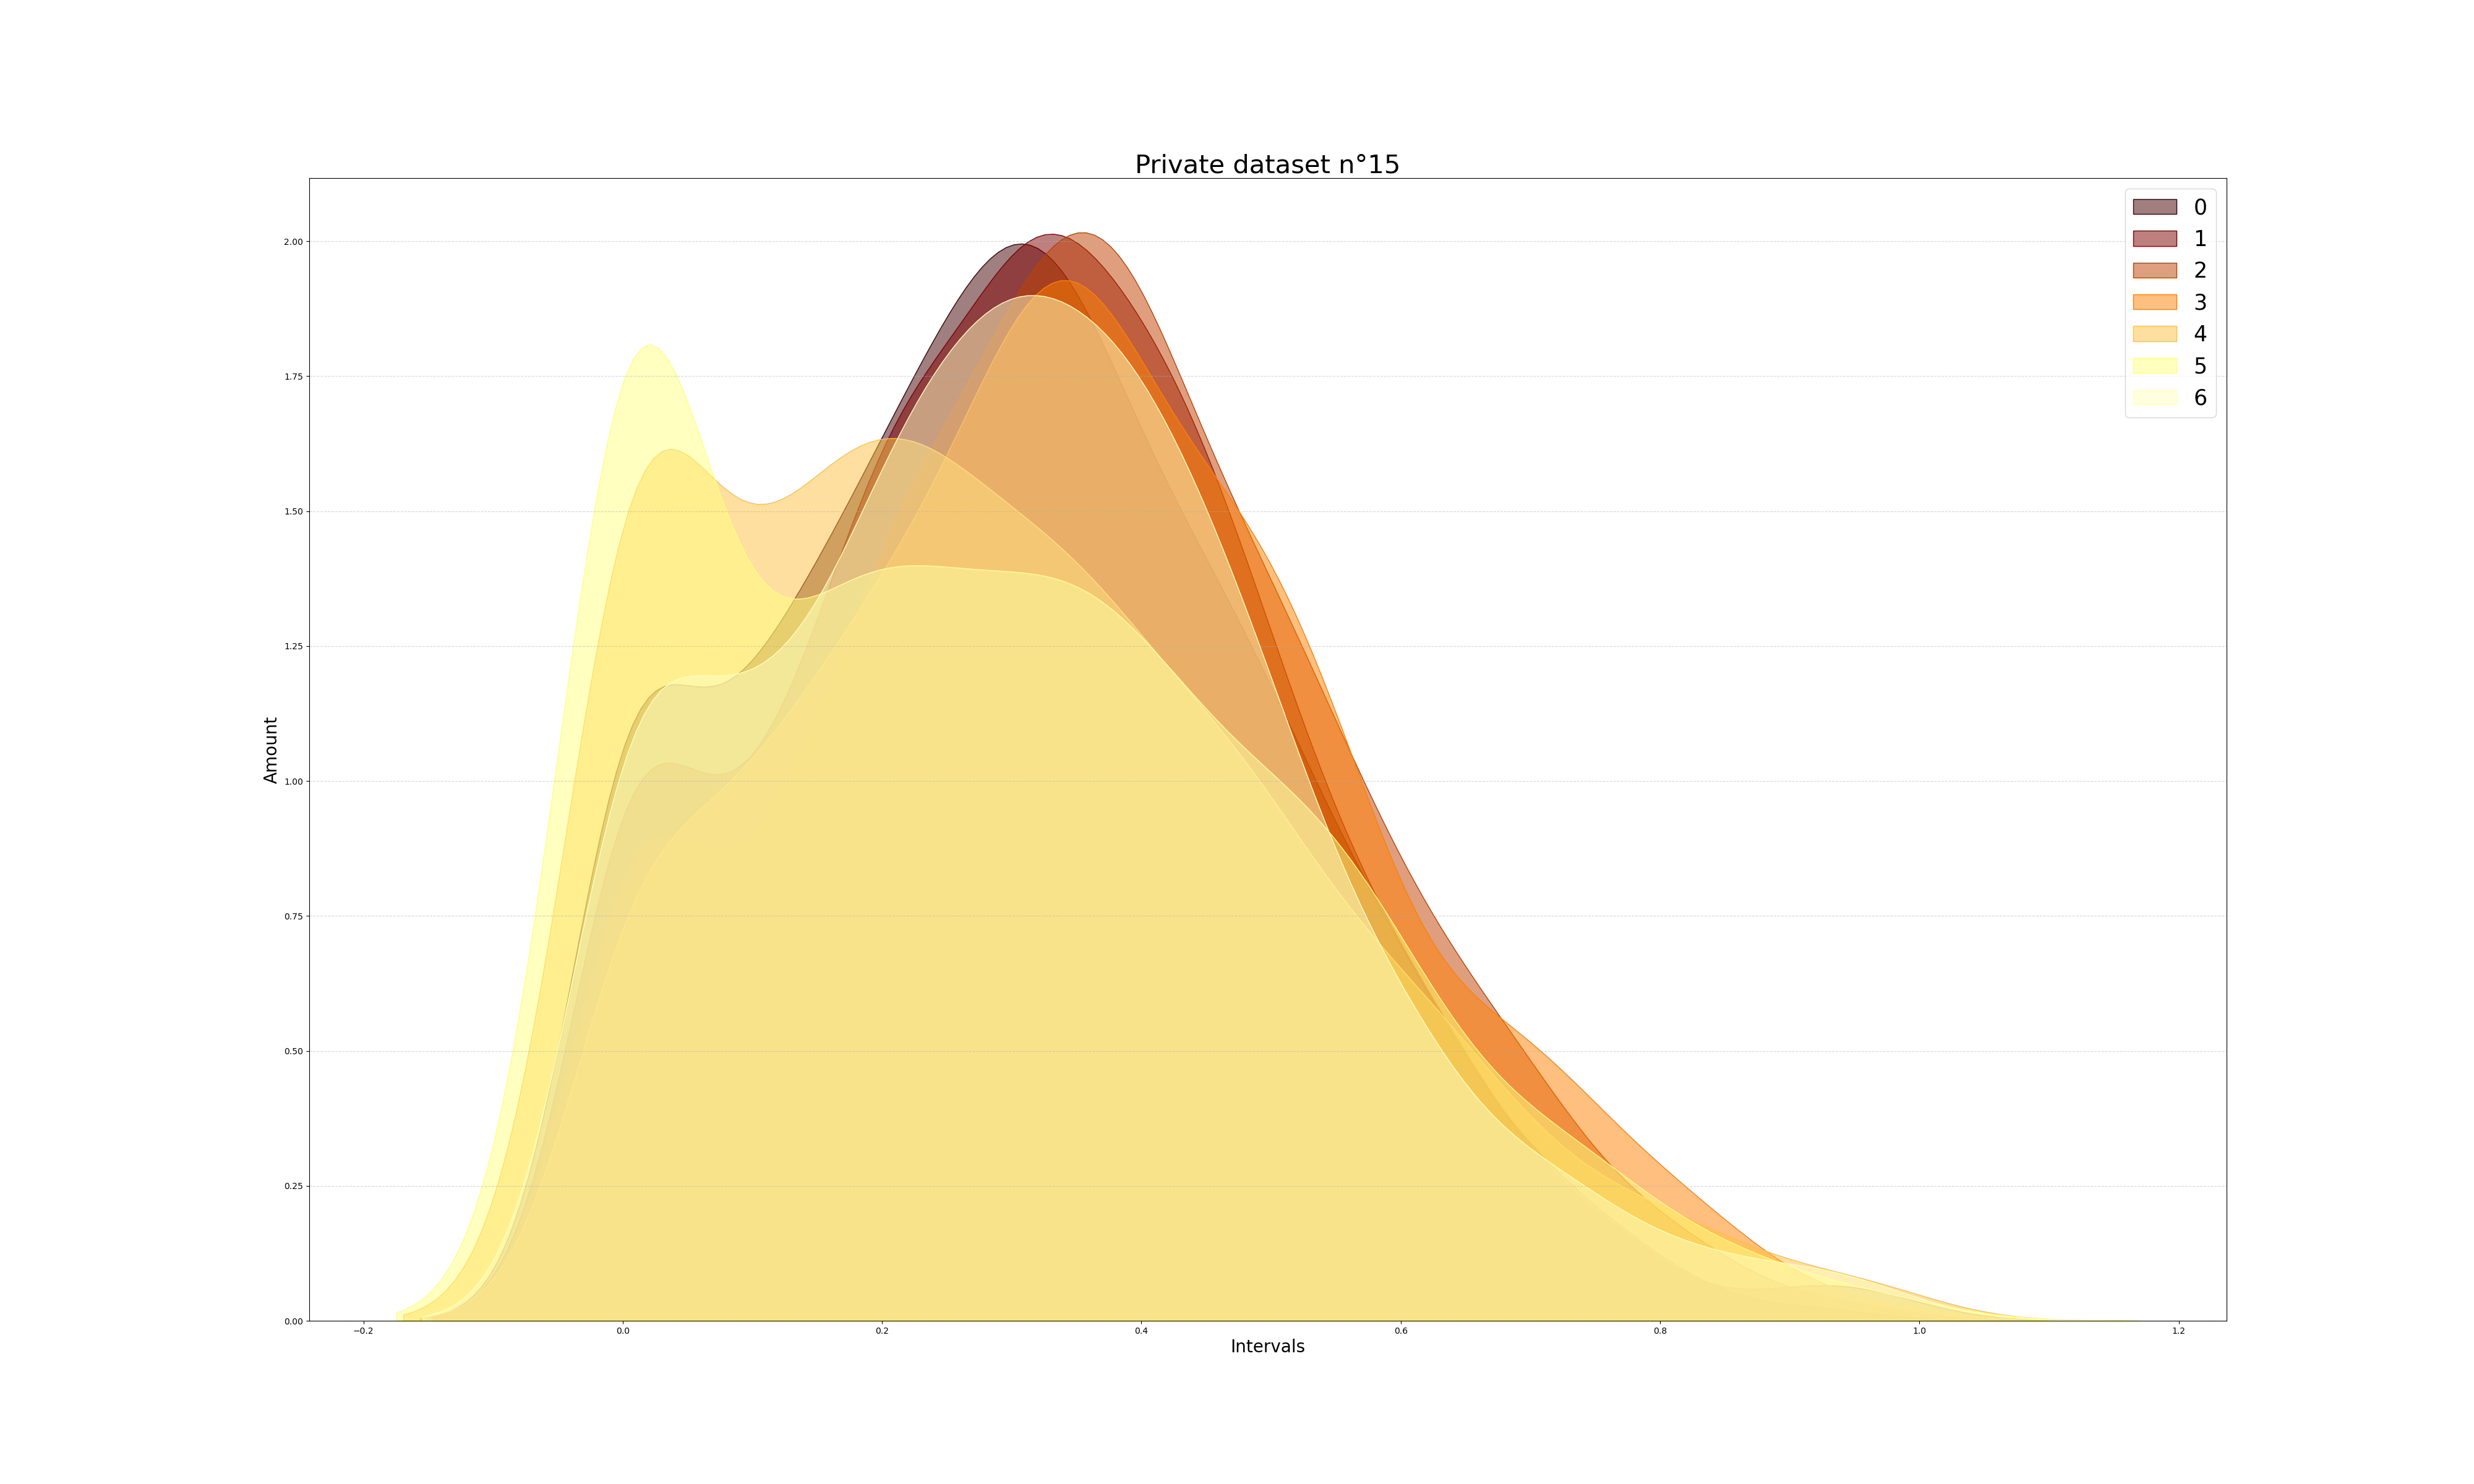
\includegraphics[width = 0.28\textwidth]{figures/Resultats/privateDS/Task 2/15}}}\qquad
            \caption{Distribution des datasets privés créés par l'équipe
                -
                $\mathfrak H\left( \mathbb{S}'_{Priv_{i_{T_{2}}}}\right) \Bigm \lvert \left(E_{T_2, \overline C, l_{30}}\right)$}
            \label{H15Priv}
        \end{figure}

        \begin{figure}[H]
            \centering
            \subfloat[]{\fbox{
                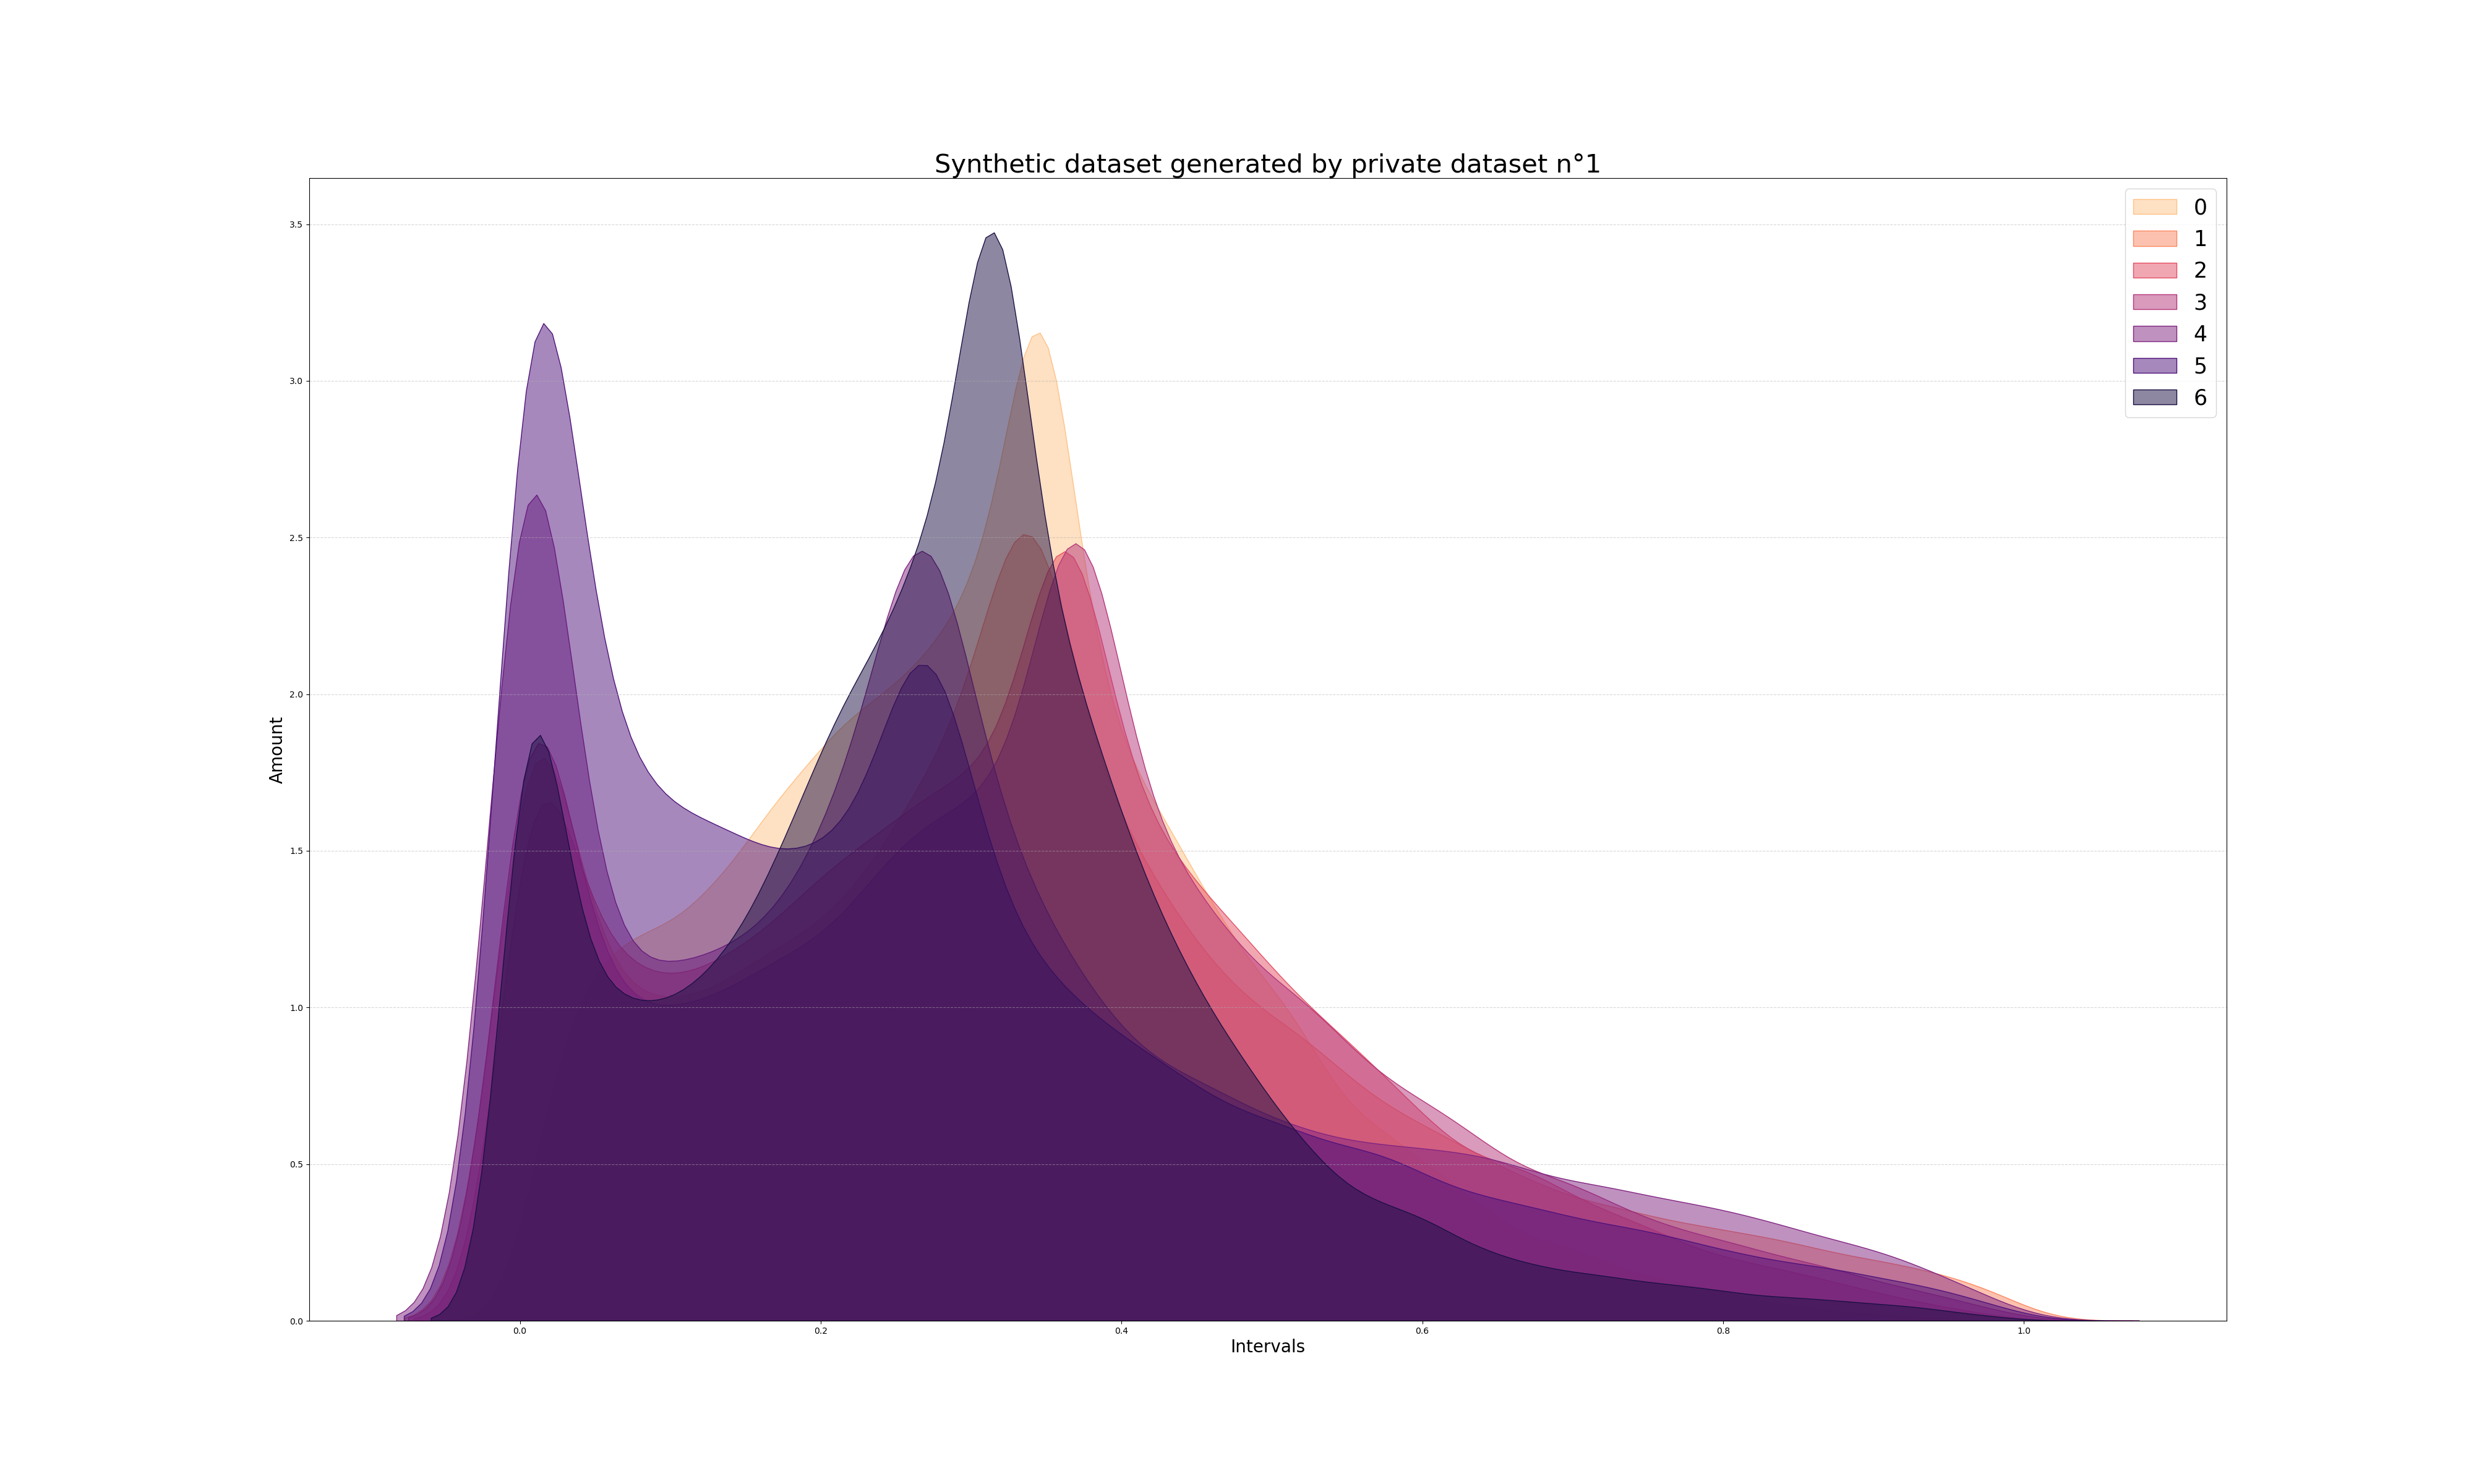
\includegraphics[width = 0.28\textwidth]{figures/Resultats/SyntheticDS/False Synthetics/Task 2/1}}}\qquad
            \subfloat[]{\fbox{
                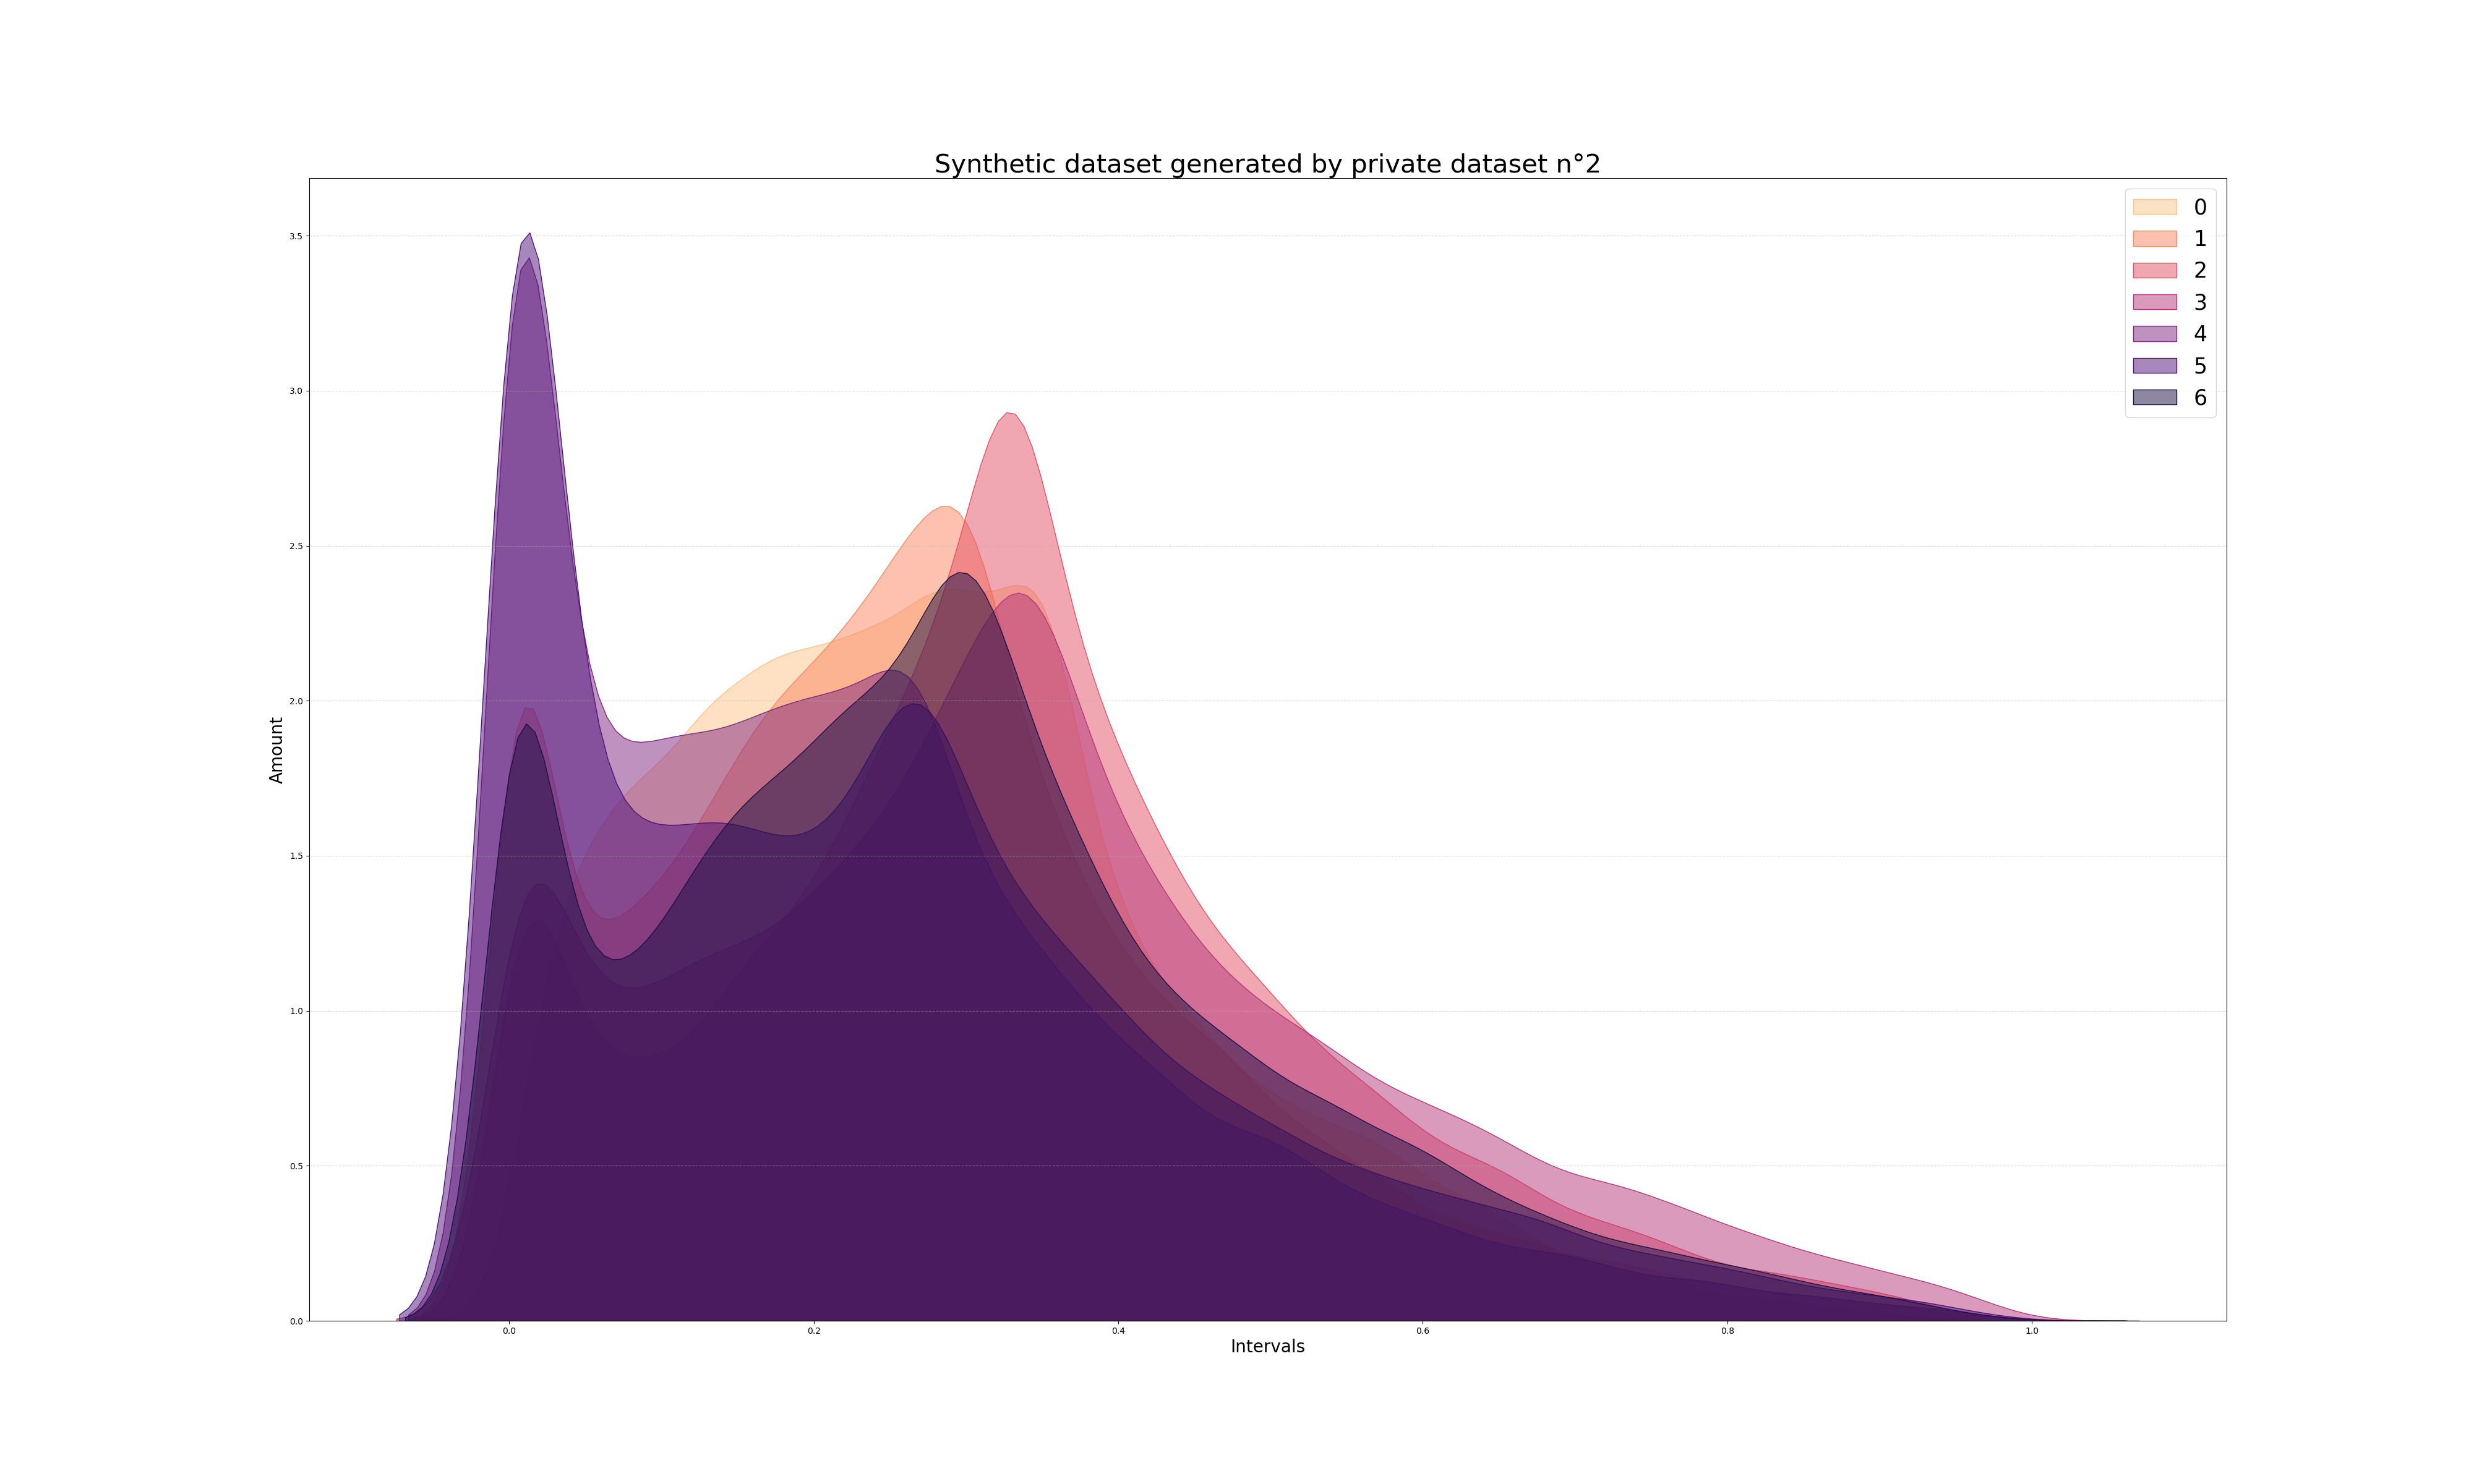
\includegraphics[width = 0.28\textwidth]{figures/Resultats/SyntheticDS/False Synthetics/Task 2/2}}}\qquad
            \subfloat[]{\fbox{
                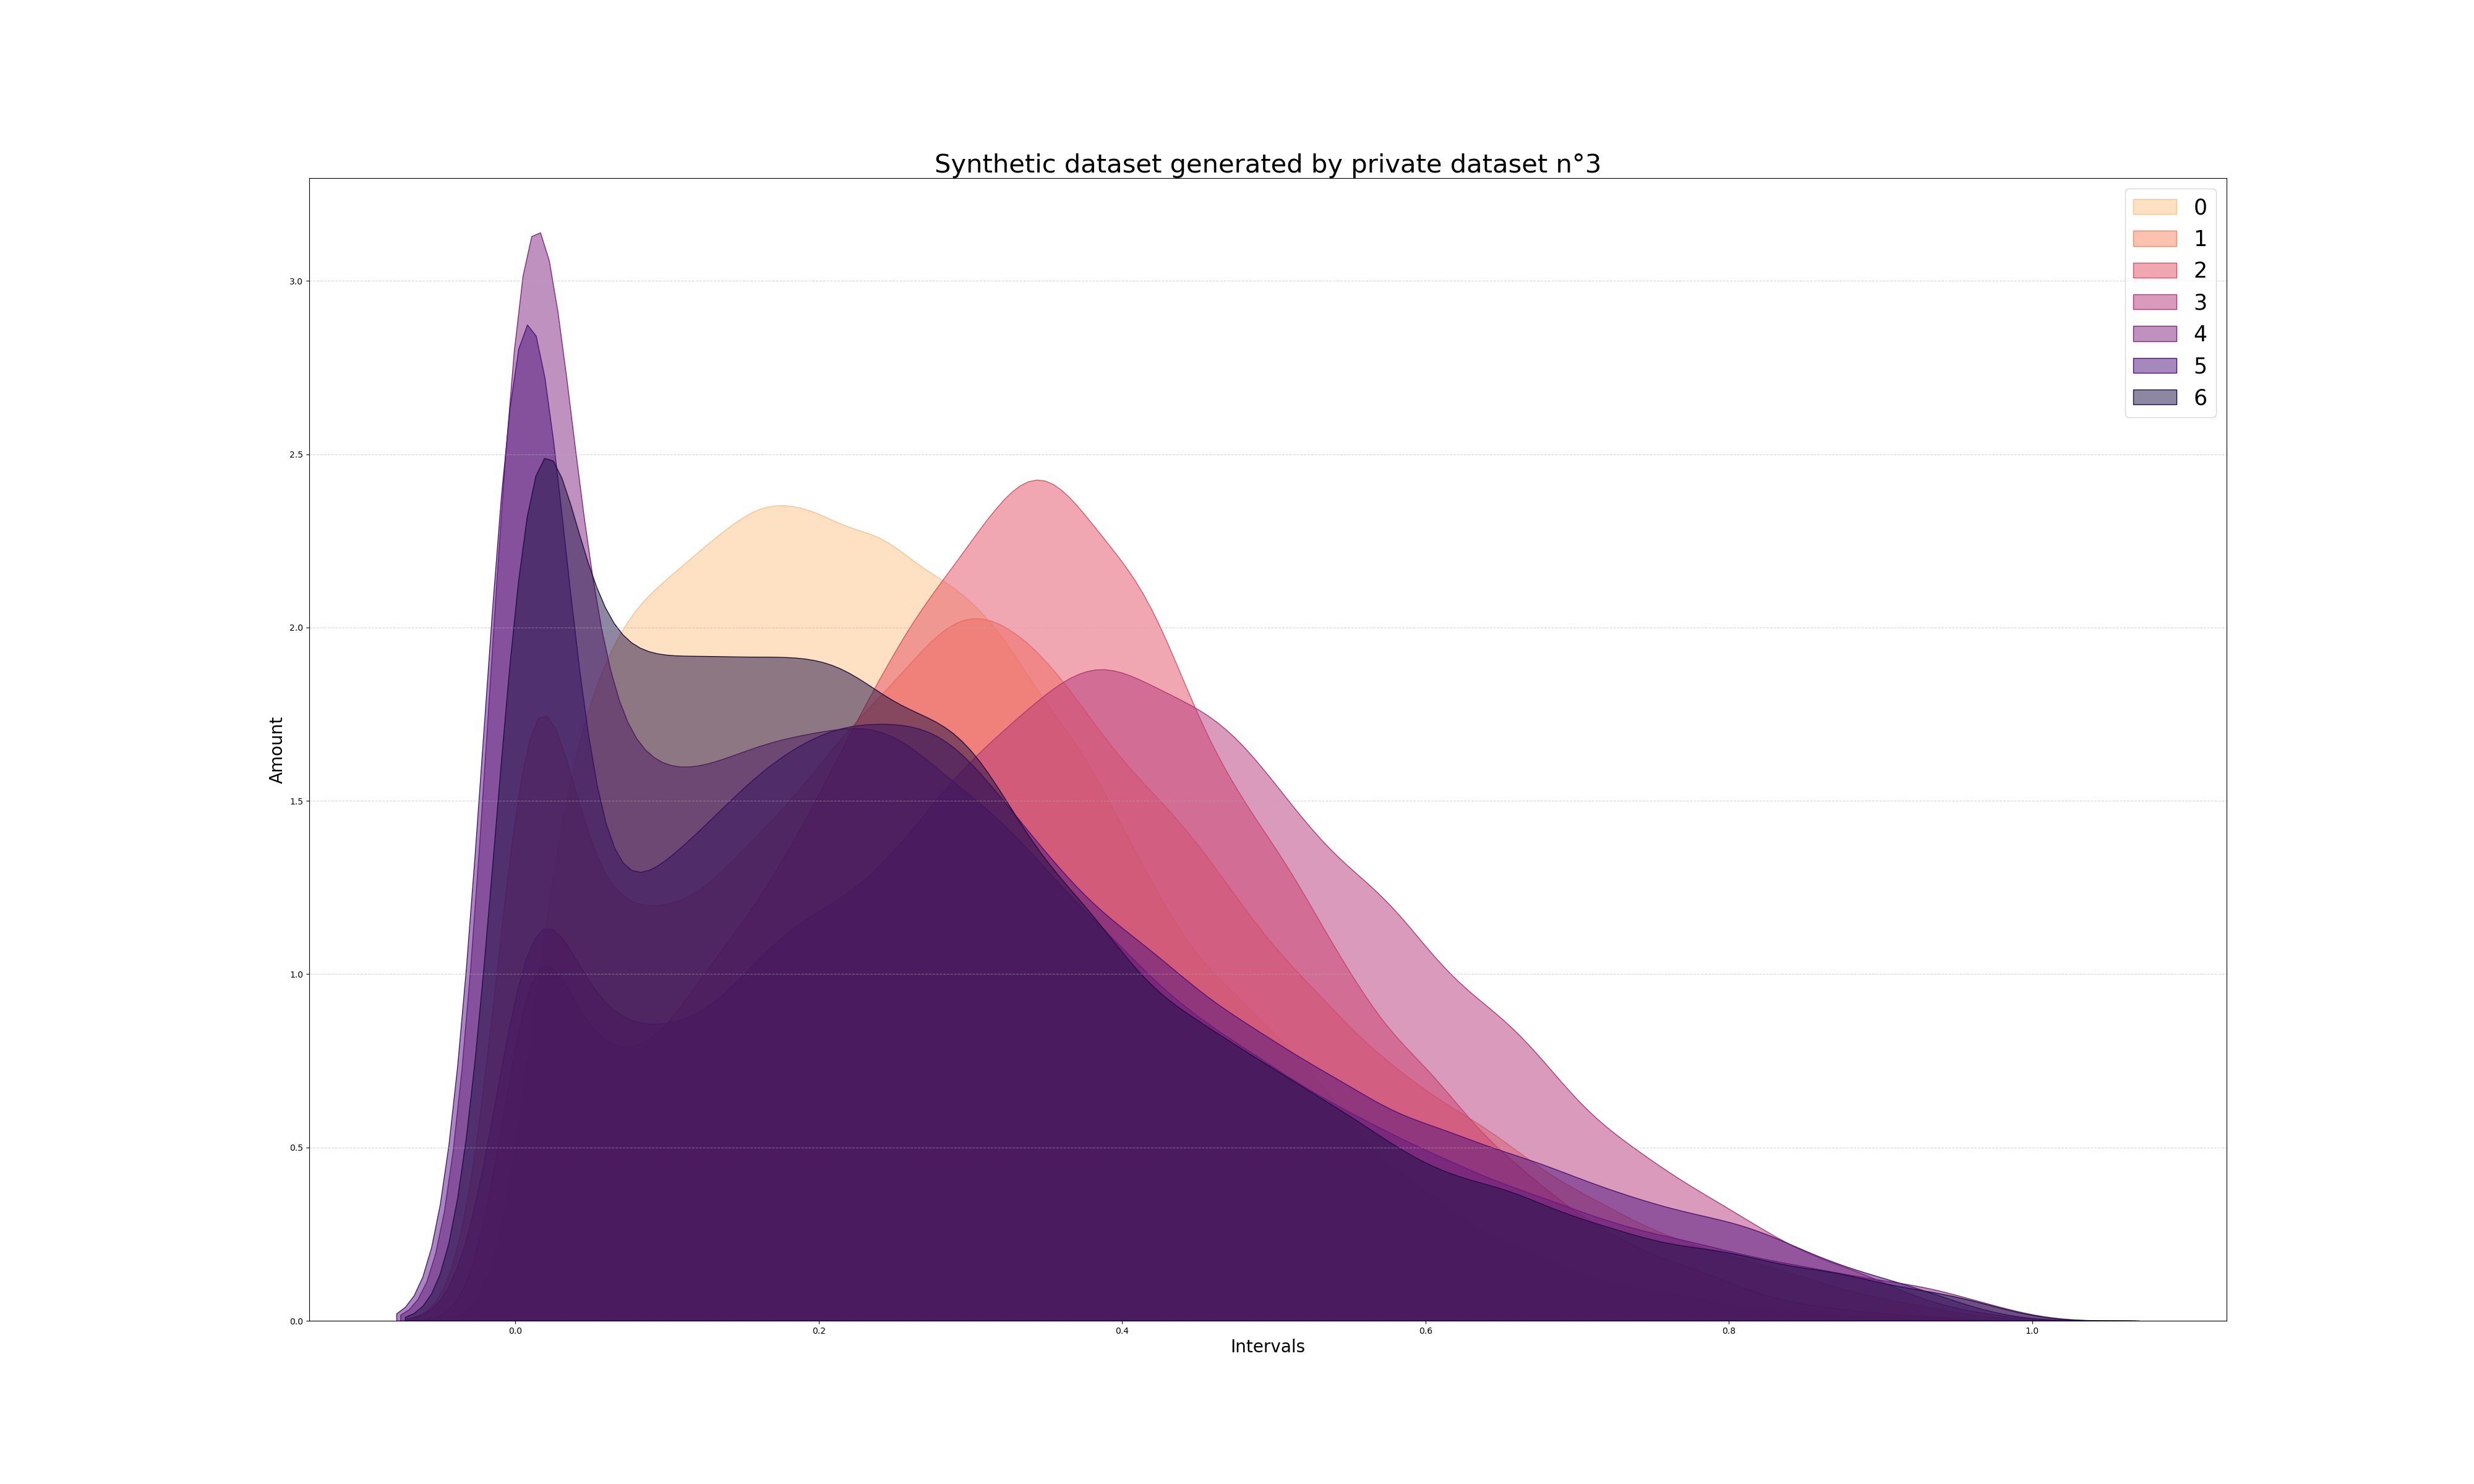
\includegraphics[width = 0.28\textwidth]{figures/Resultats/SyntheticDS/False Synthetics/Task 2/3}}}\qquad
            \subfloat[]{\fbox{
                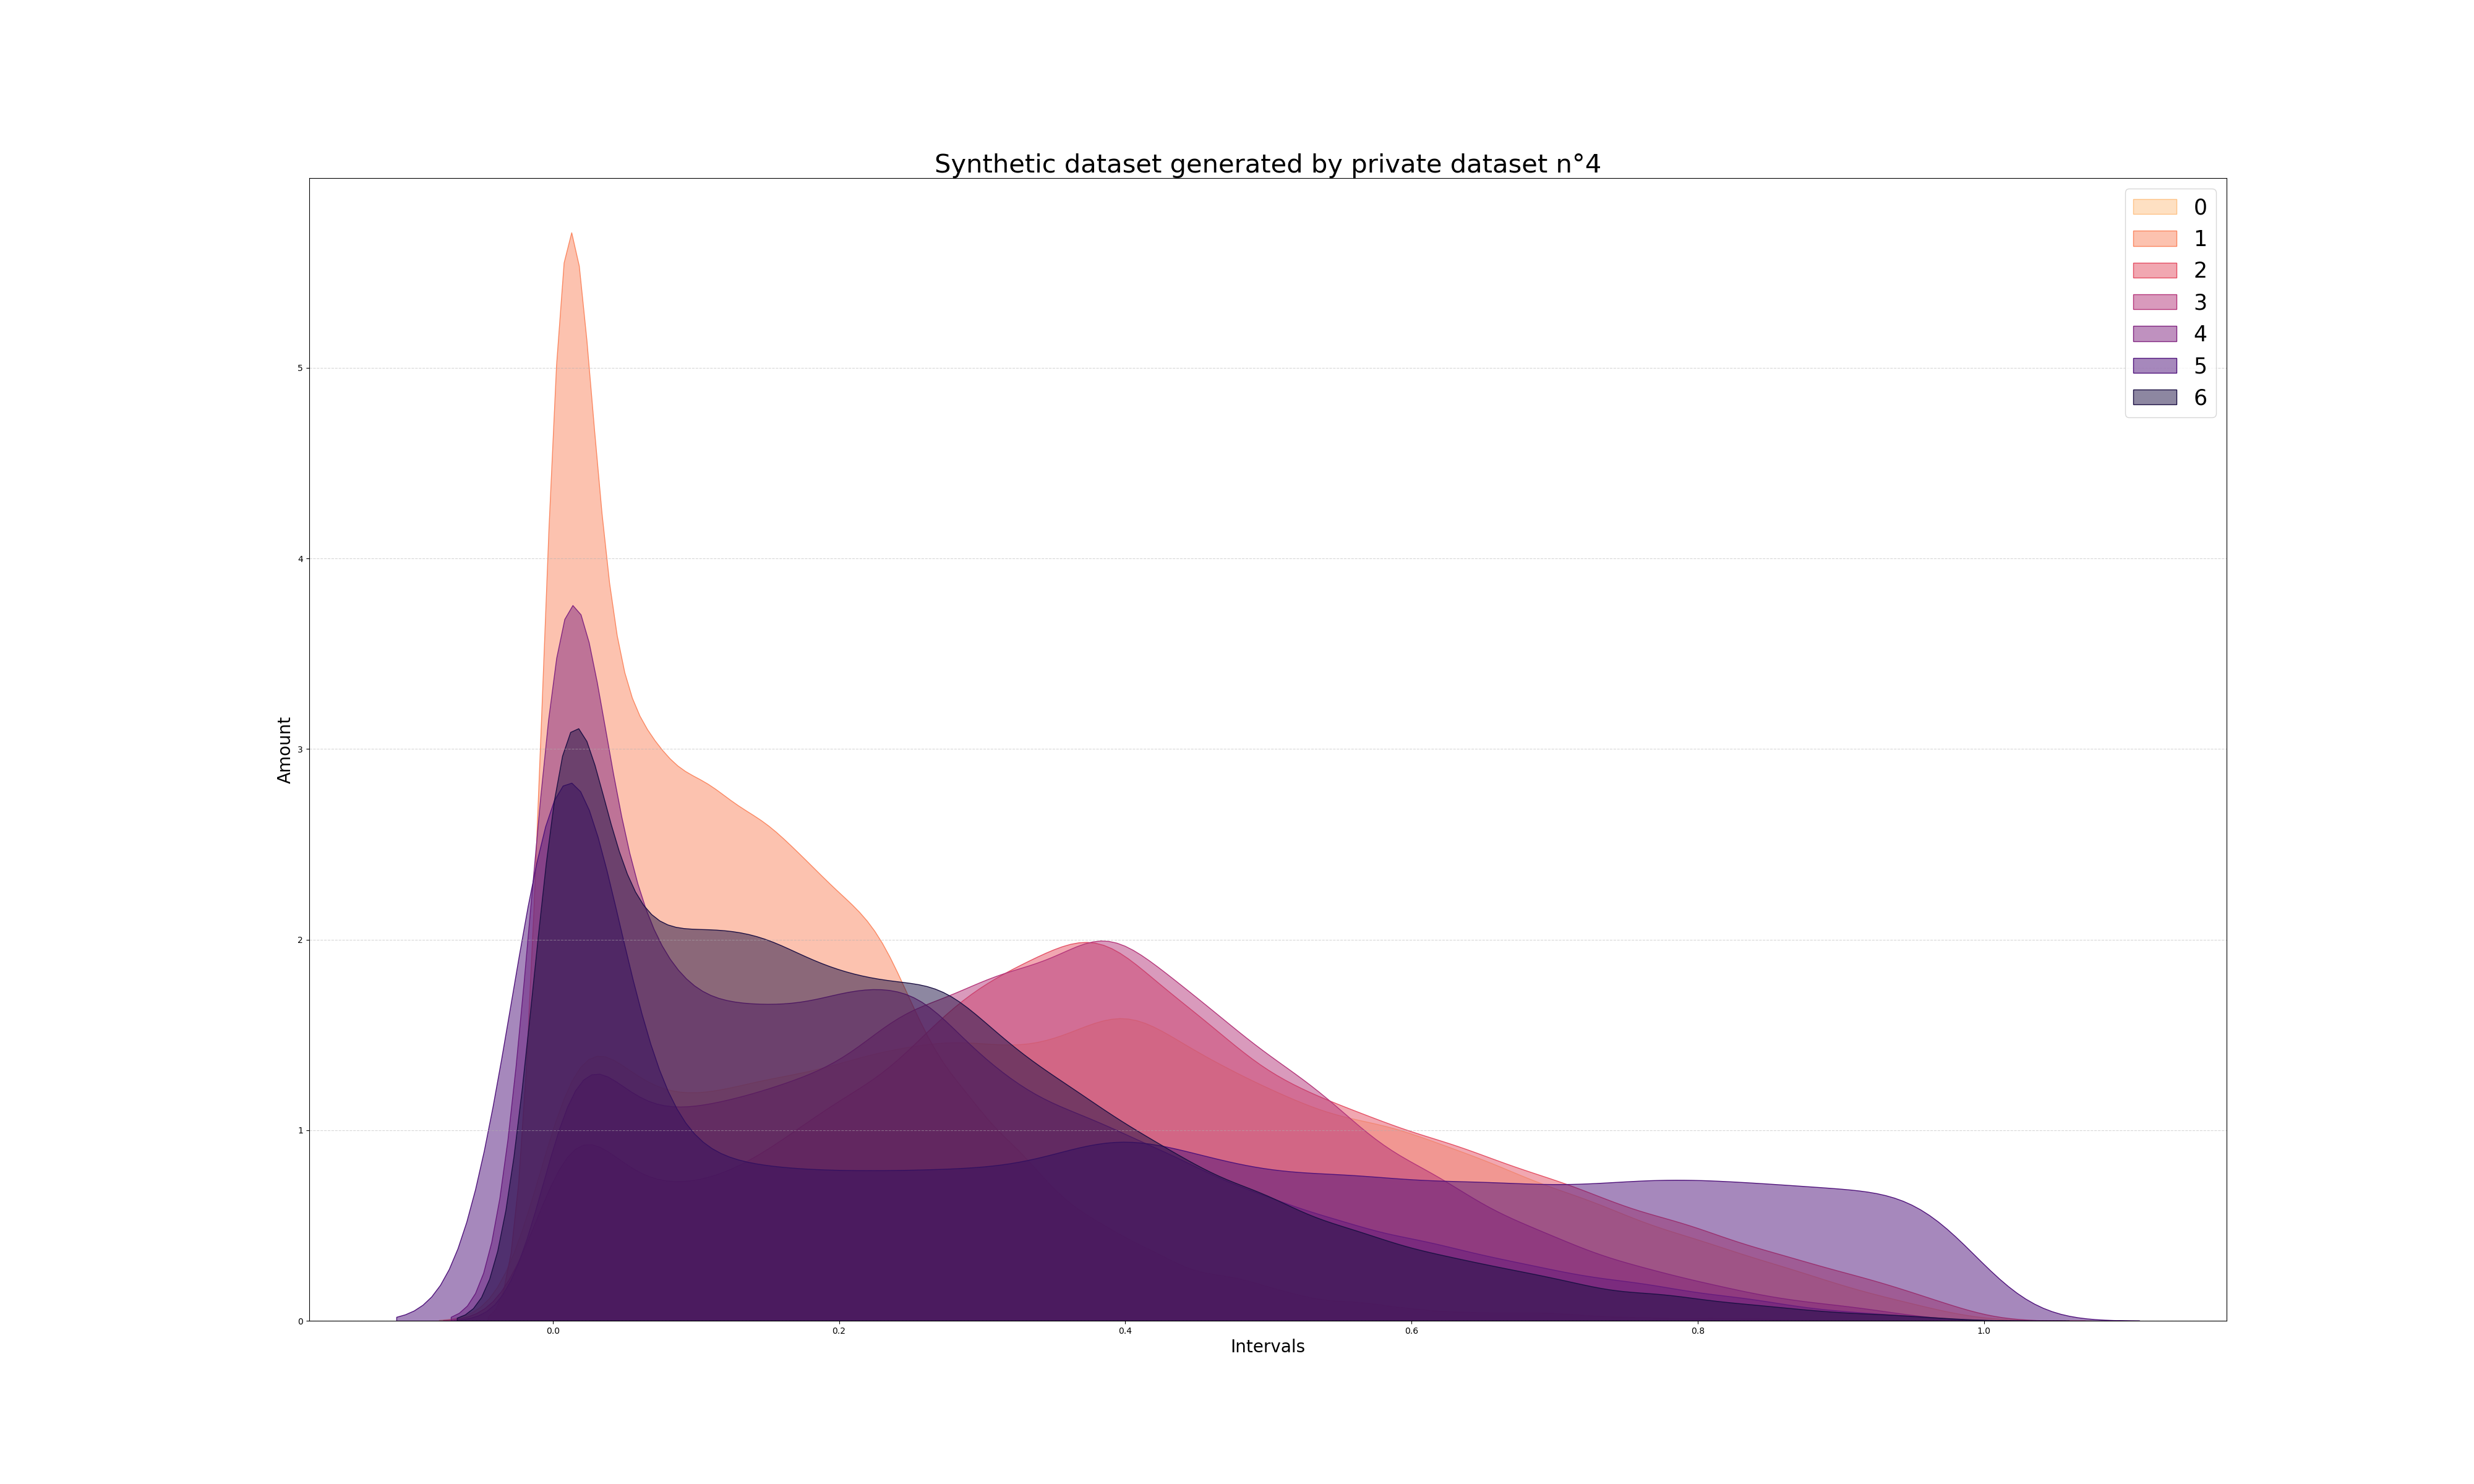
\includegraphics[width = 0.28\textwidth]{figures/Resultats/SyntheticDS/False Synthetics/Task 2/4}}}\qquad
            \subfloat[]{\fbox{
                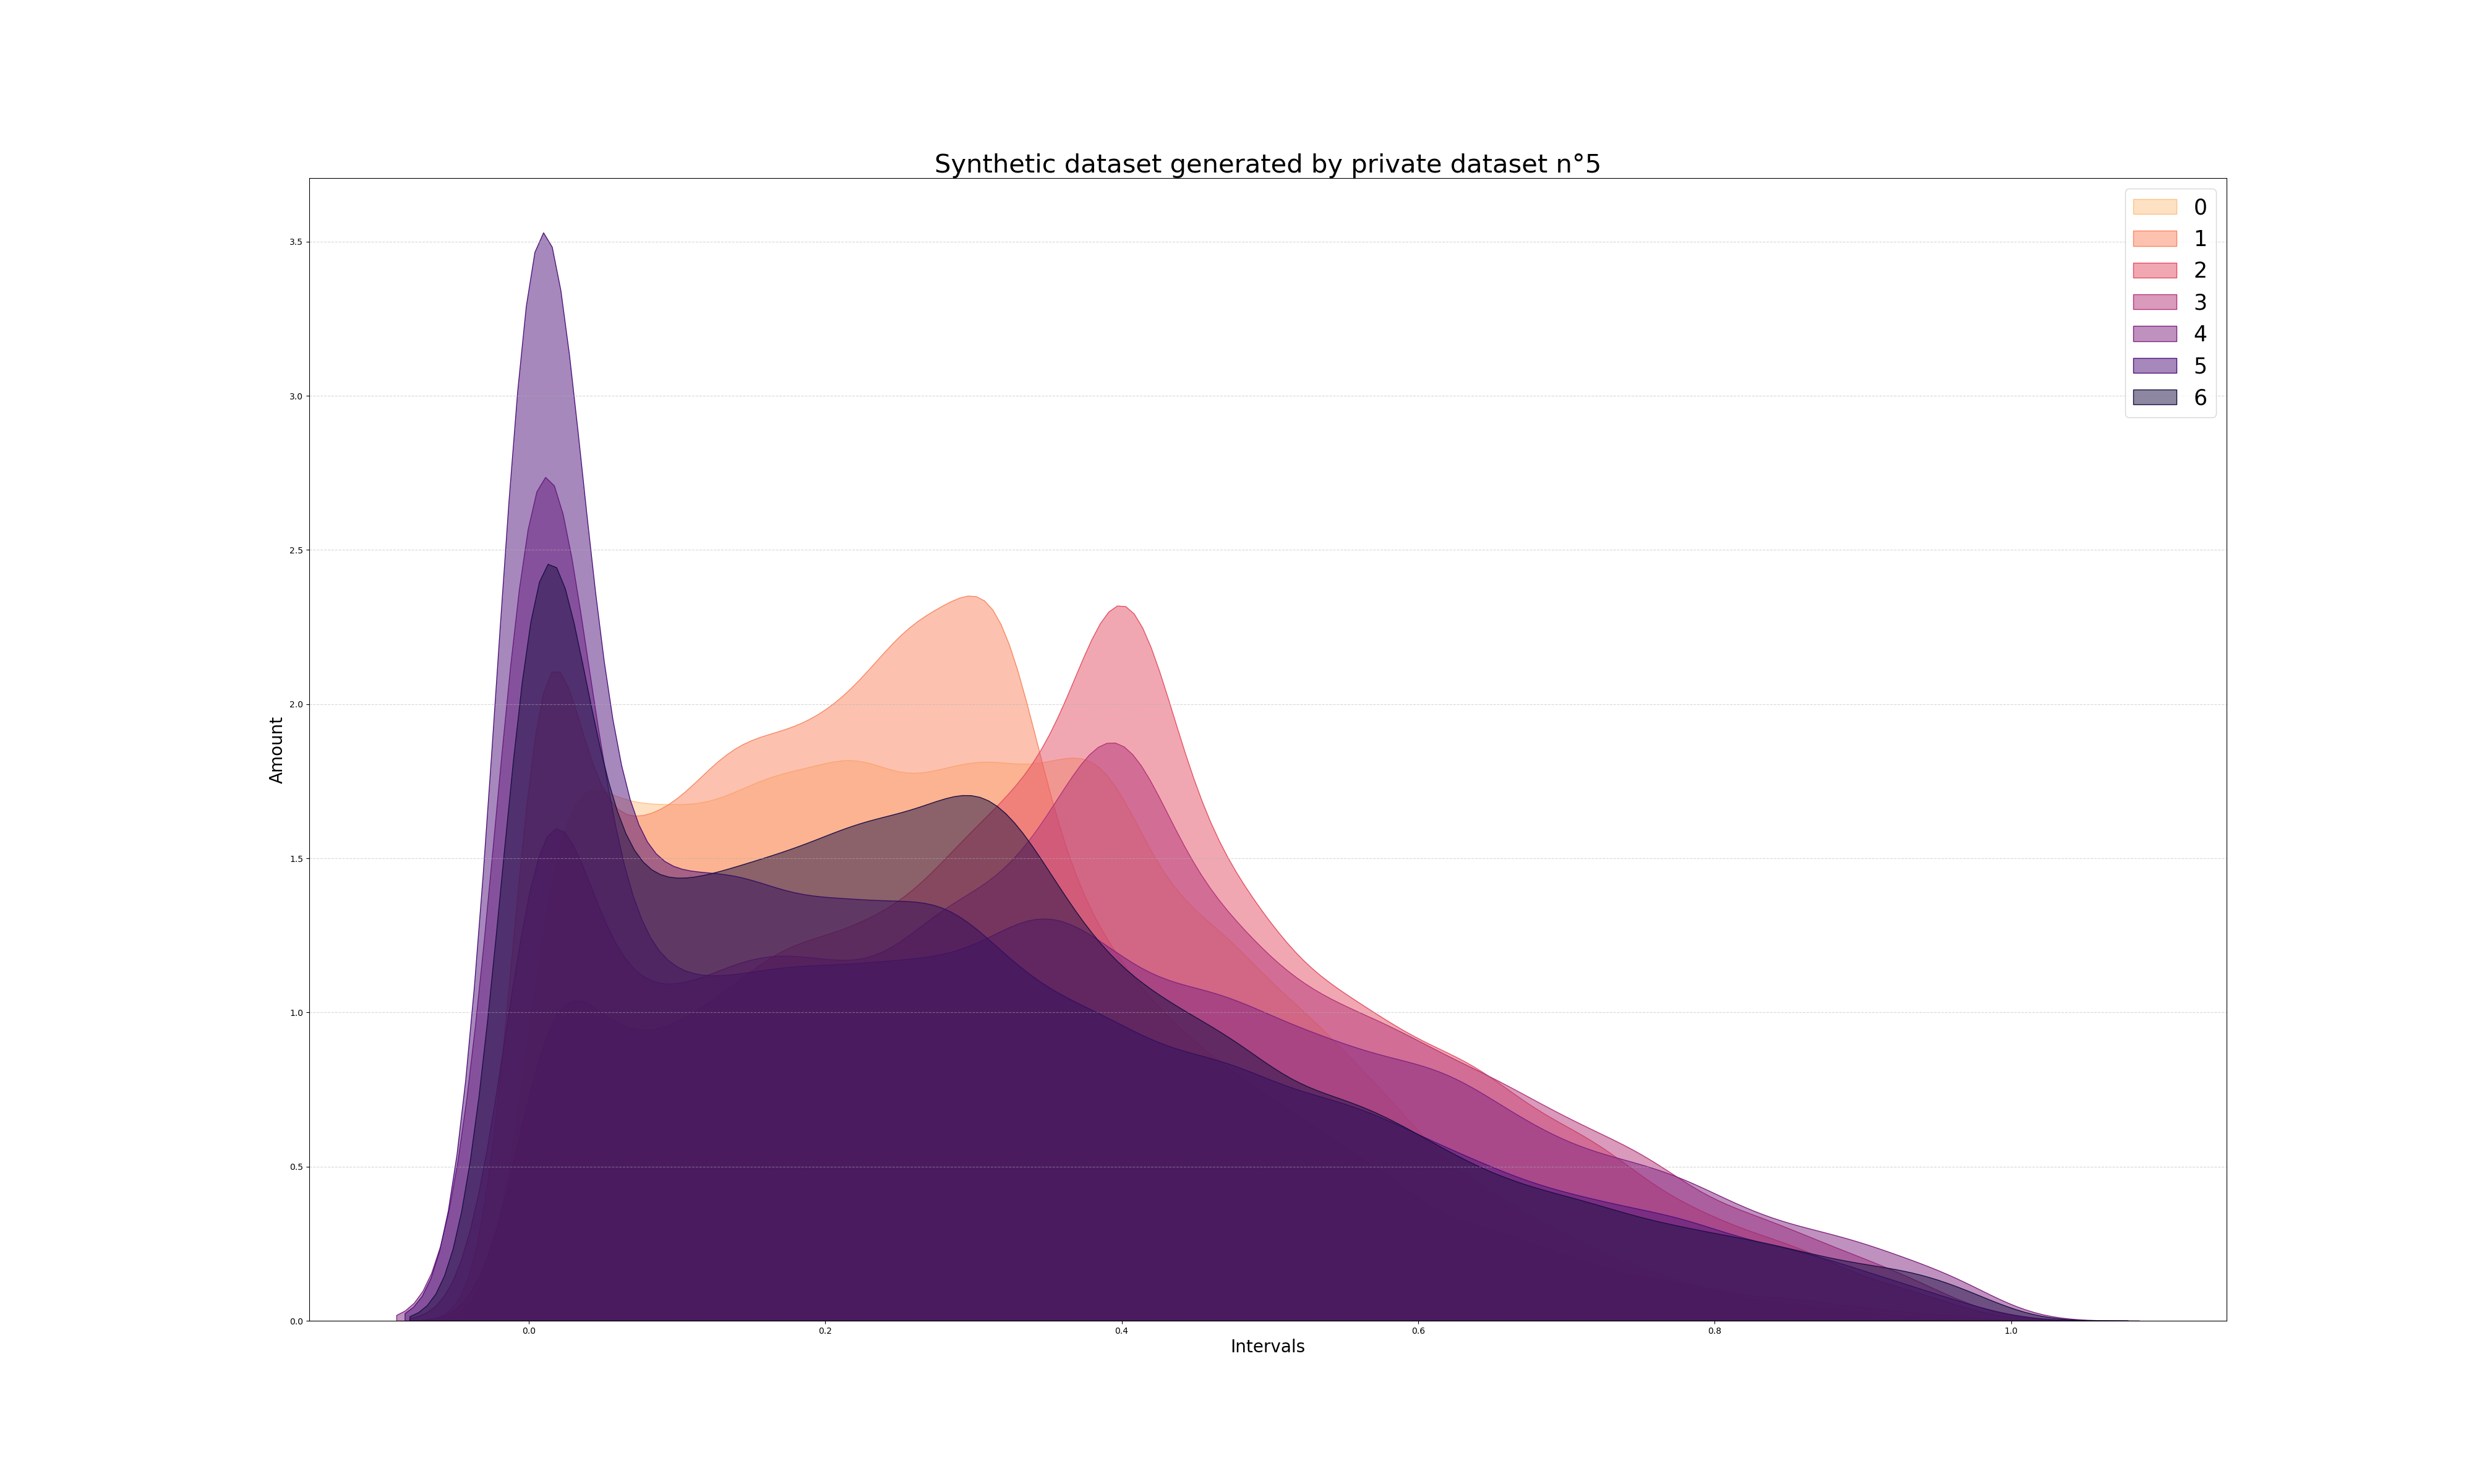
\includegraphics[width = 0.28\textwidth]{figures/Resultats/SyntheticDS/False Synthetics/Task 2/5}}}\qquad
            \subfloat[]{\fbox{
                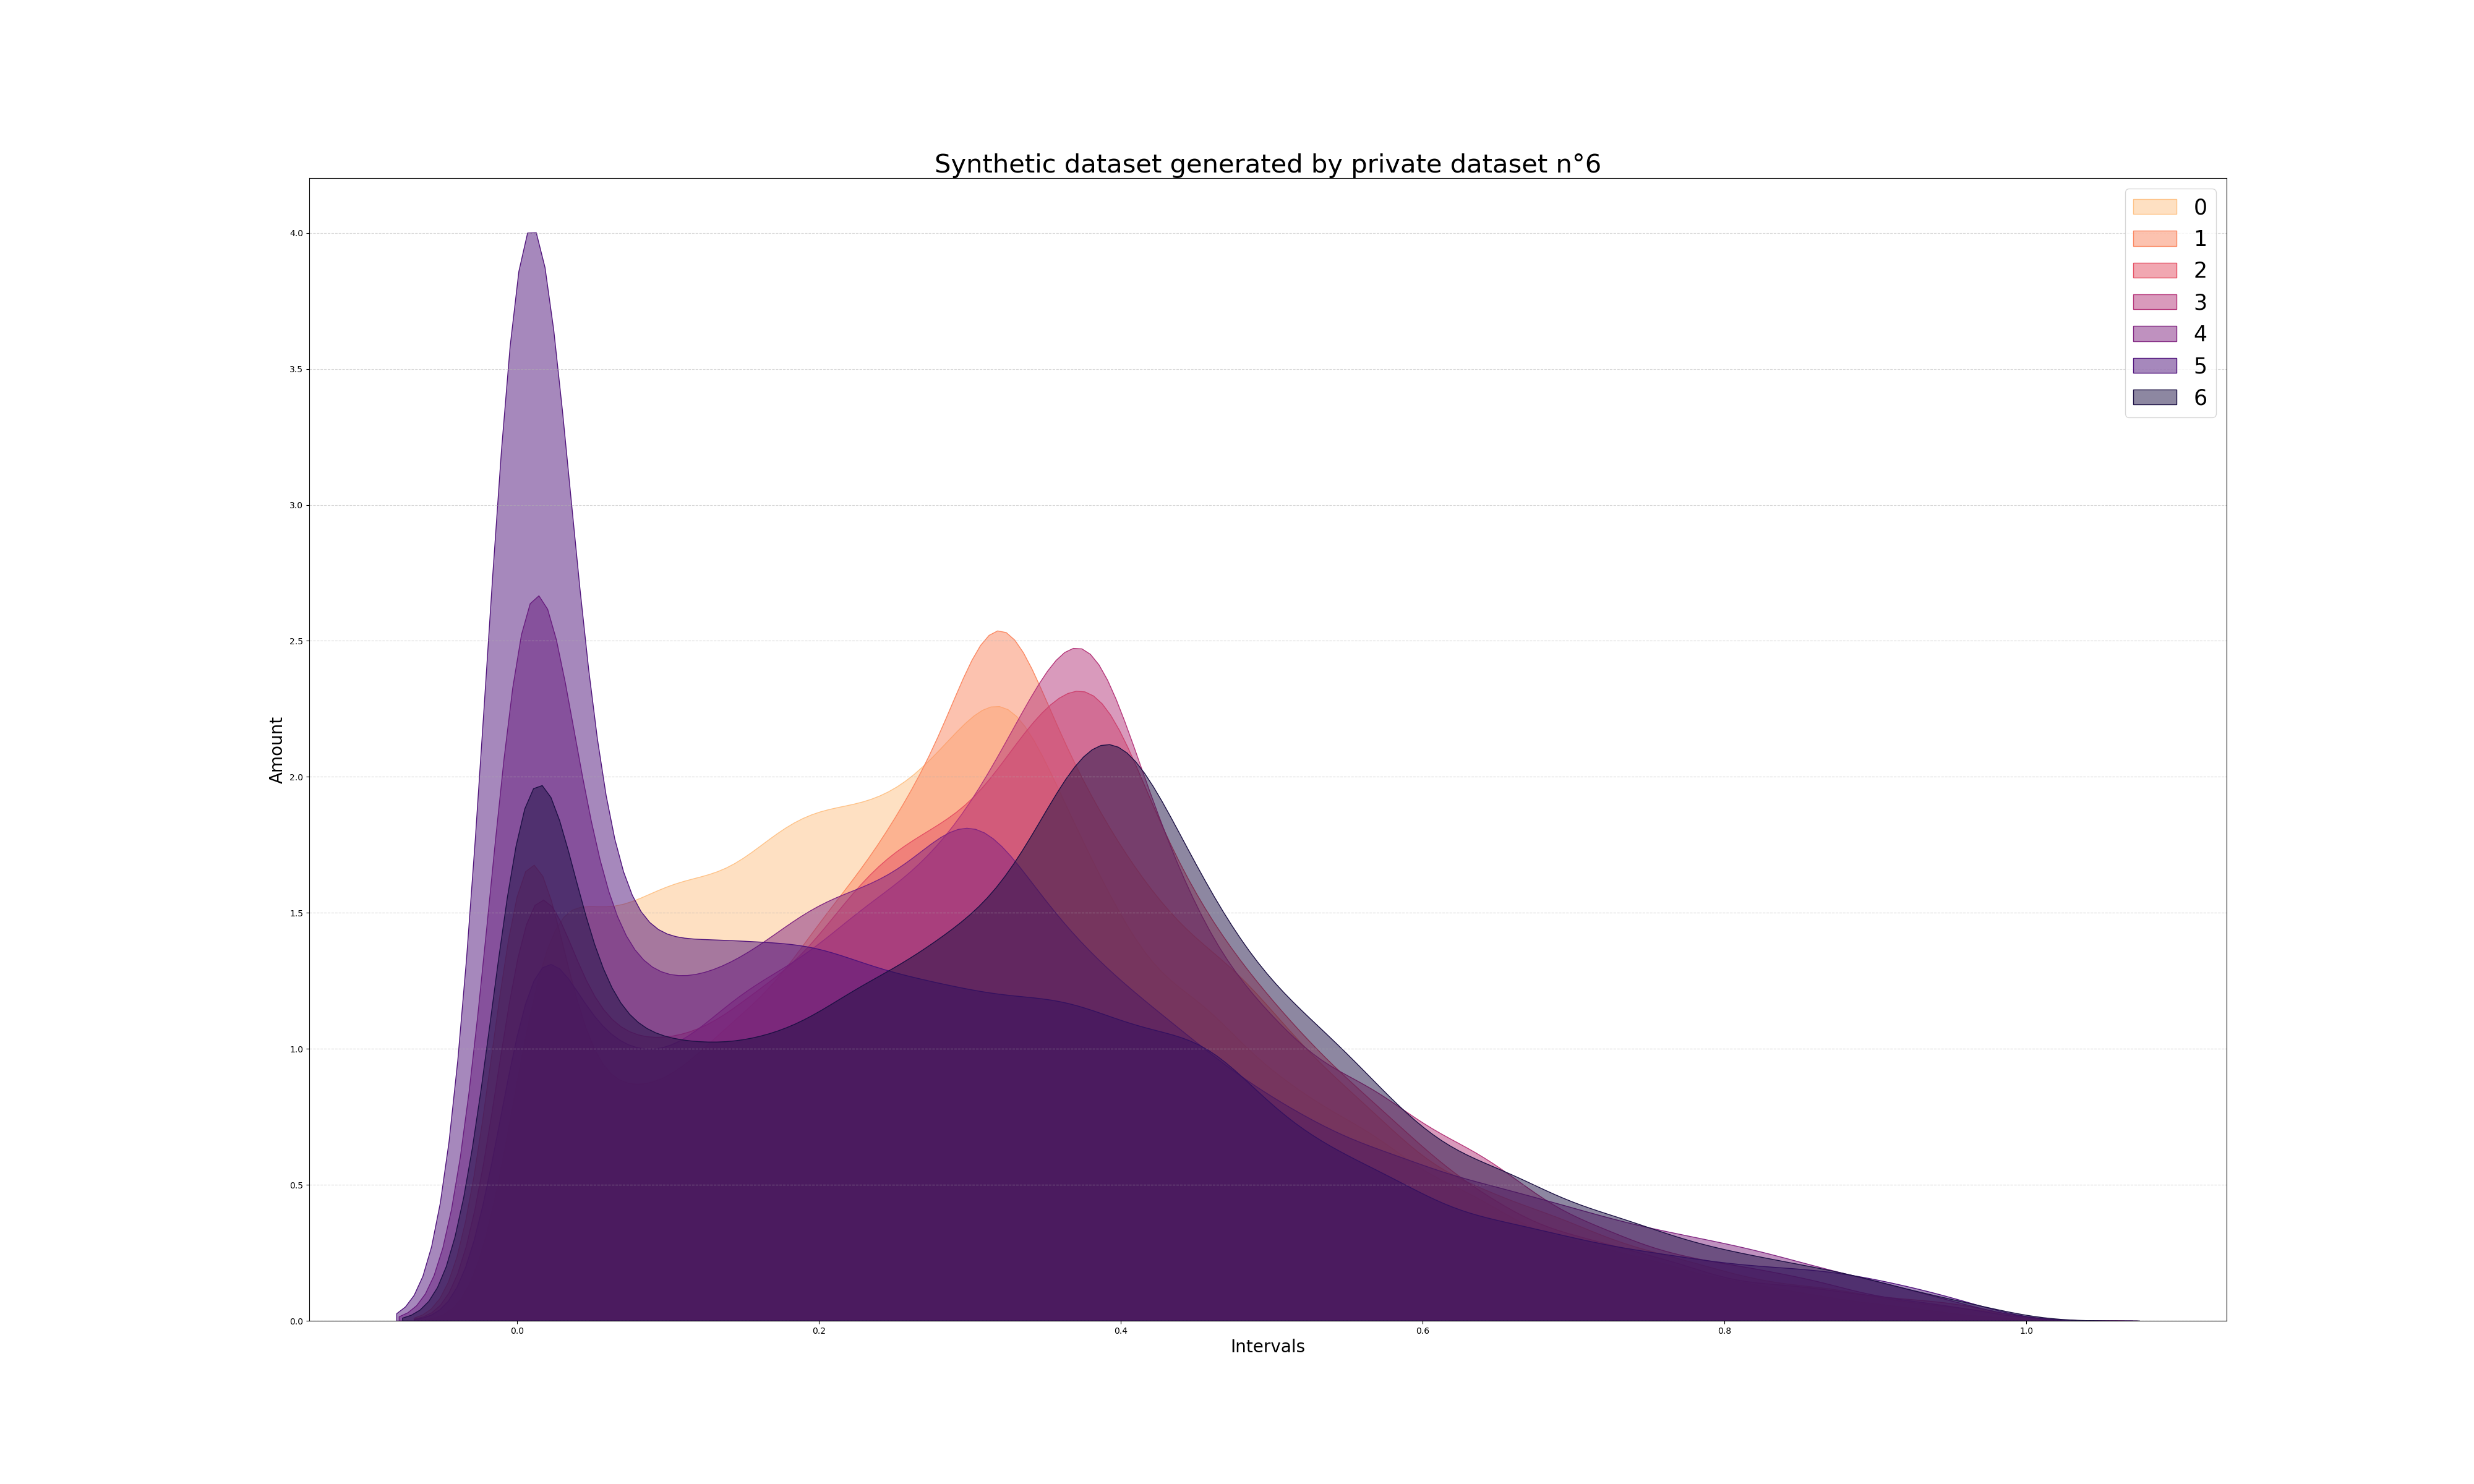
\includegraphics[width = 0.28\textwidth]{figures/Resultats/SyntheticDS/False Synthetics/Task 2/6}}}\qquad
            \subfloat[]{\fbox{
                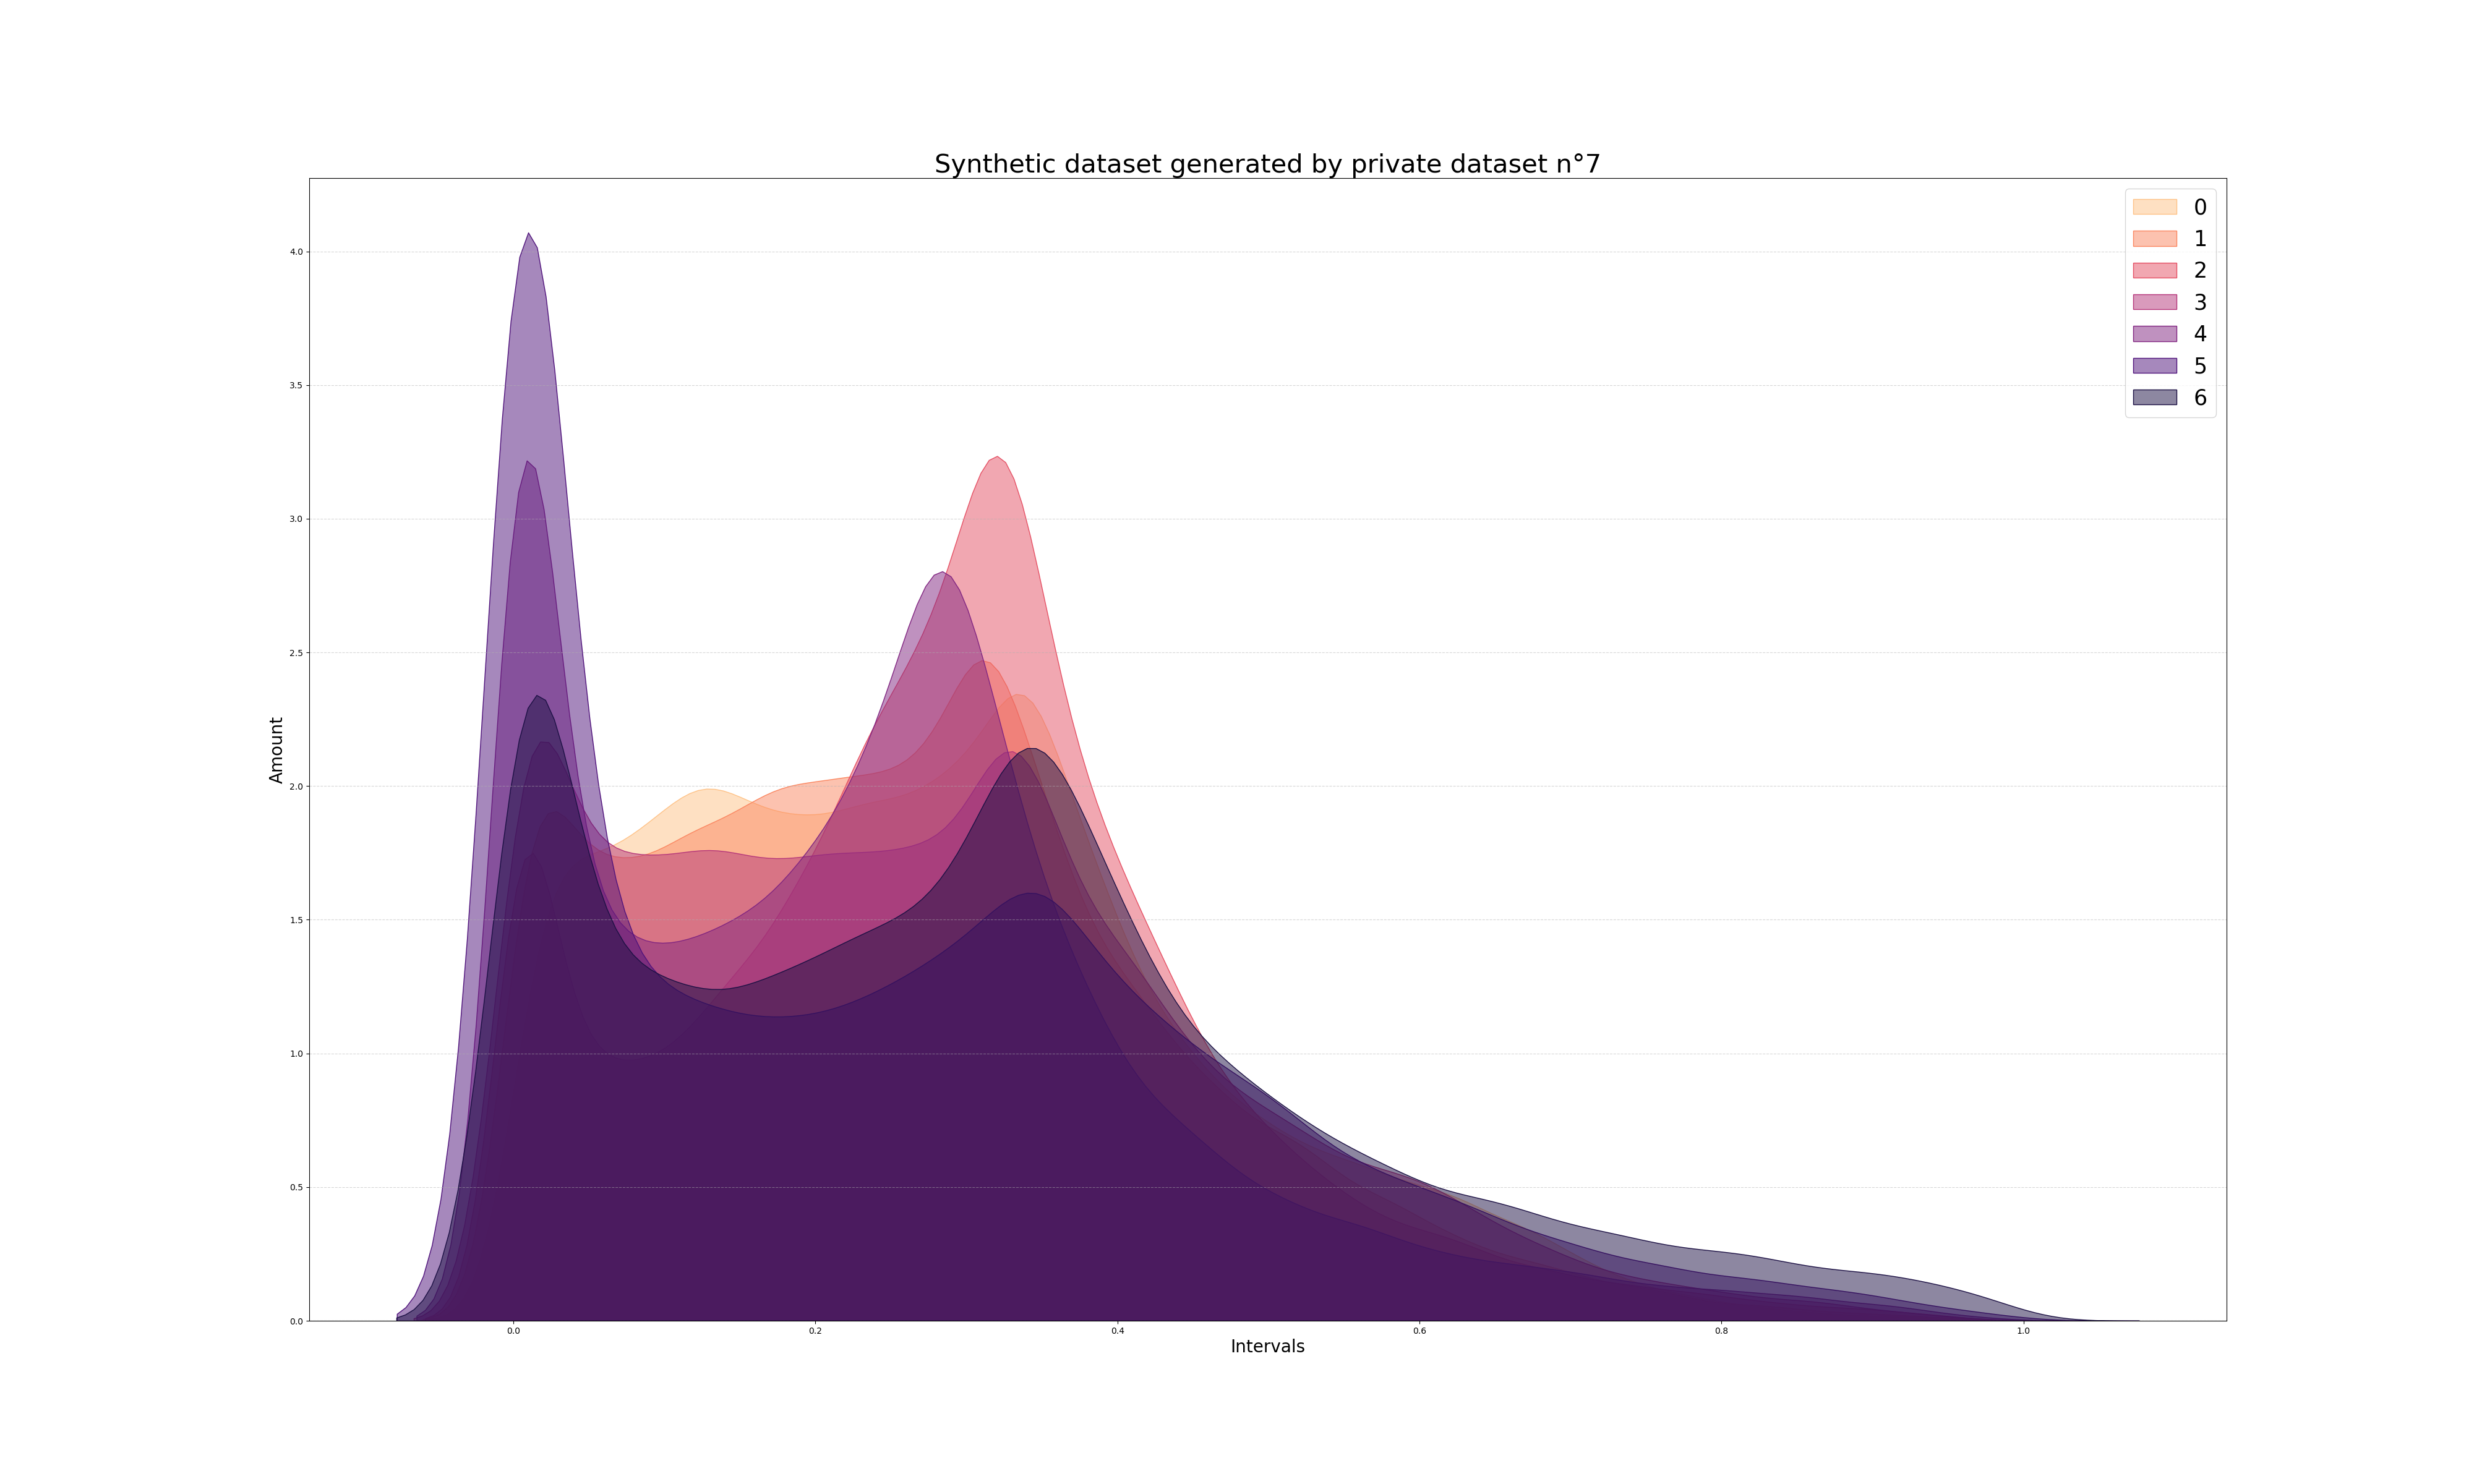
\includegraphics[width = 0.28\textwidth]{figures/Resultats/SyntheticDS/False Synthetics/Task 2/7}}}\qquad
            \subfloat[]{\fbox{
                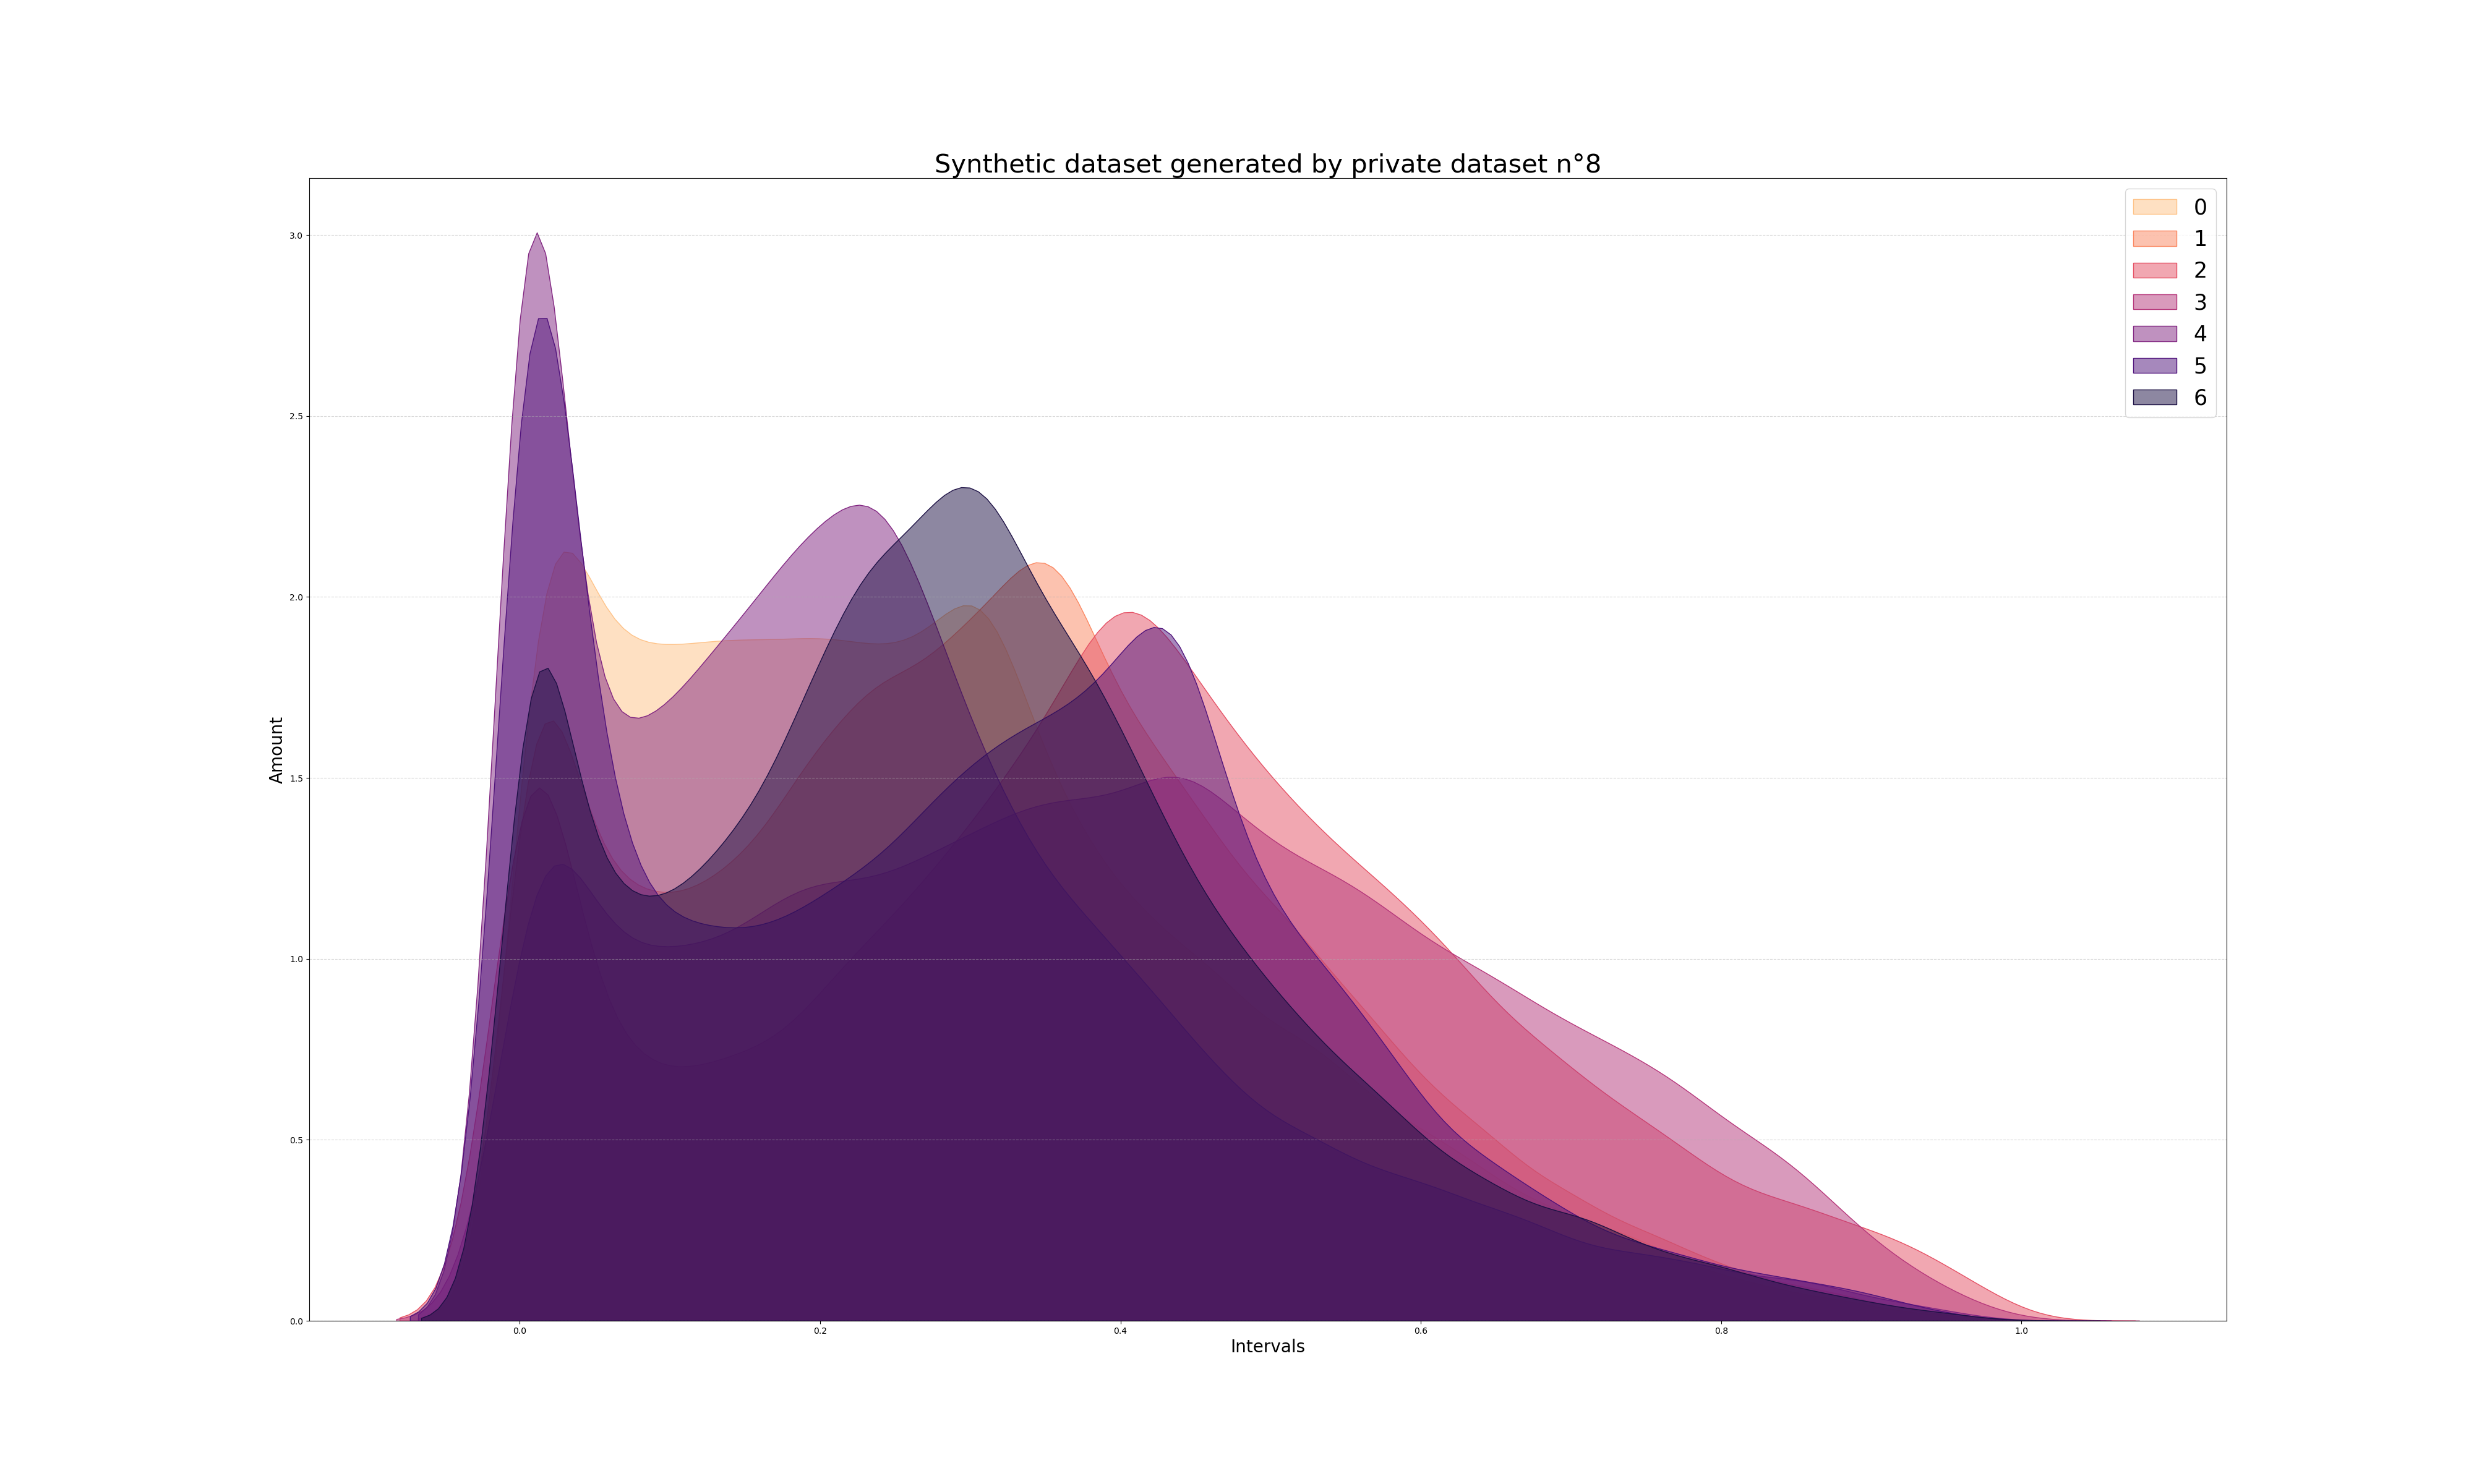
\includegraphics[width = 0.28\textwidth]{figures/Resultats/SyntheticDS/False Synthetics/Task 2/8}}}\qquad
            \subfloat[]{\fbox{
                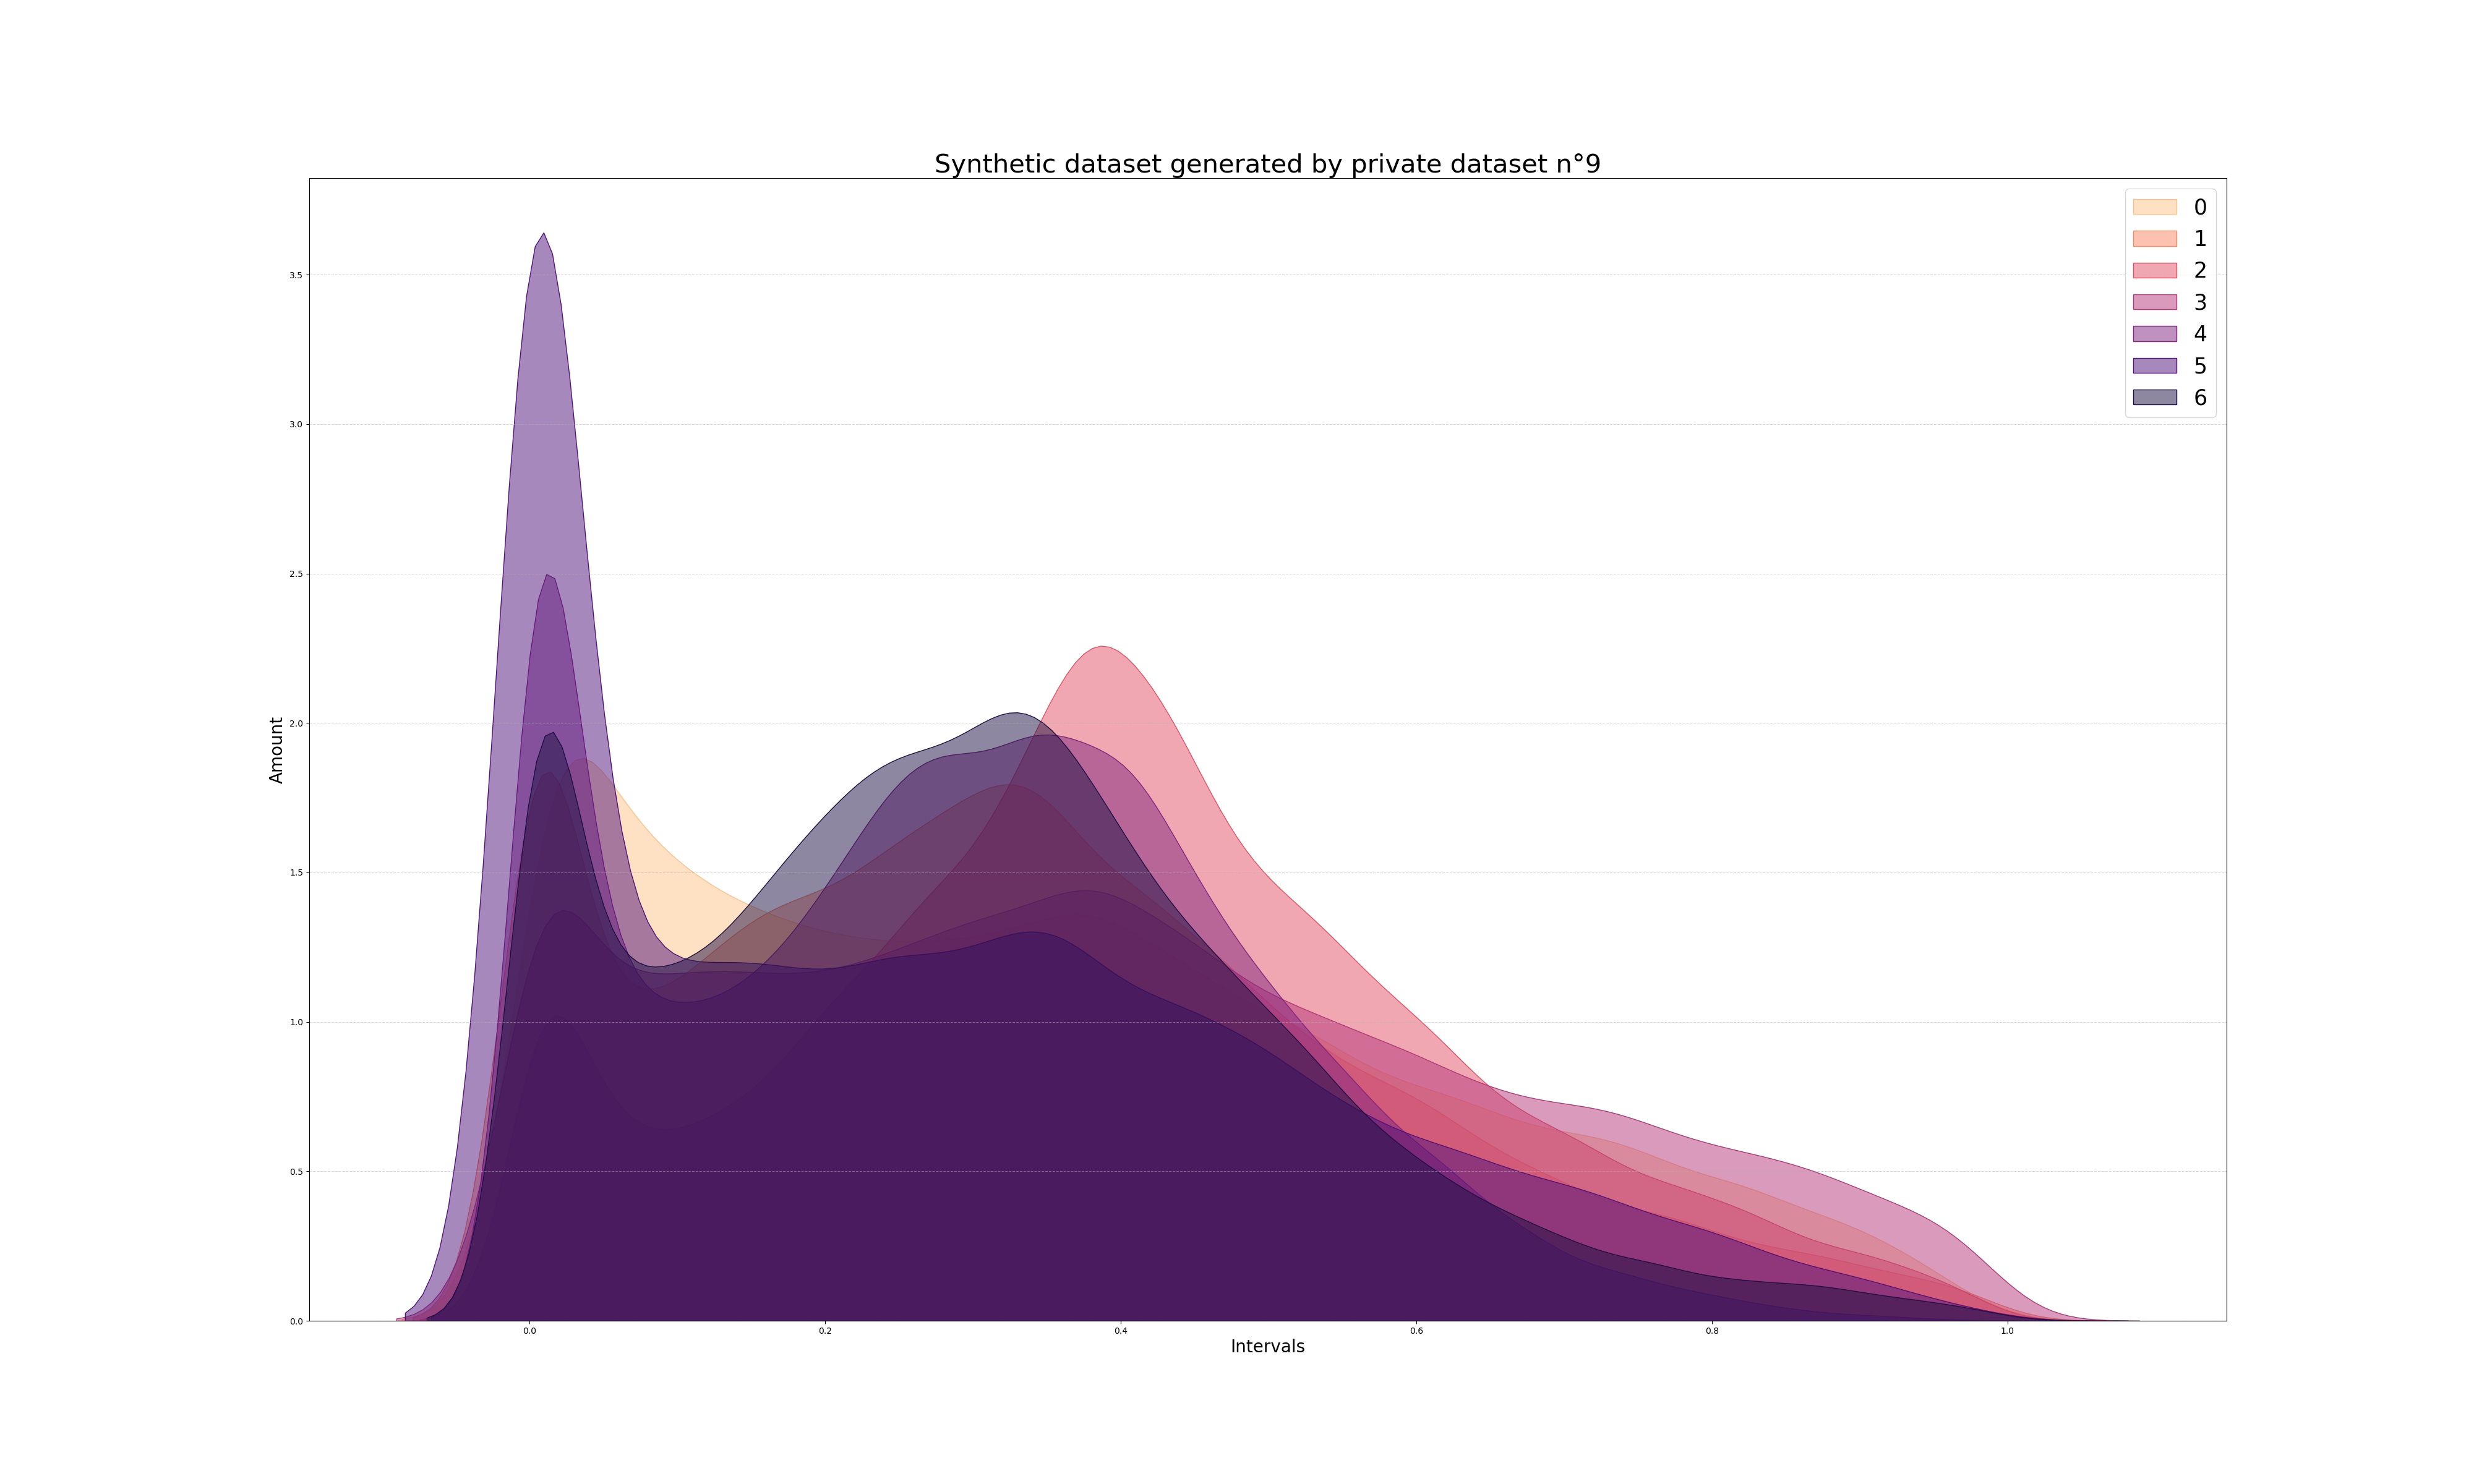
\includegraphics[width = 0.28\textwidth]{figures/Resultats/SyntheticDS/False Synthetics/Task 2/9}}}\qquad
            \subfloat[]{\fbox{
                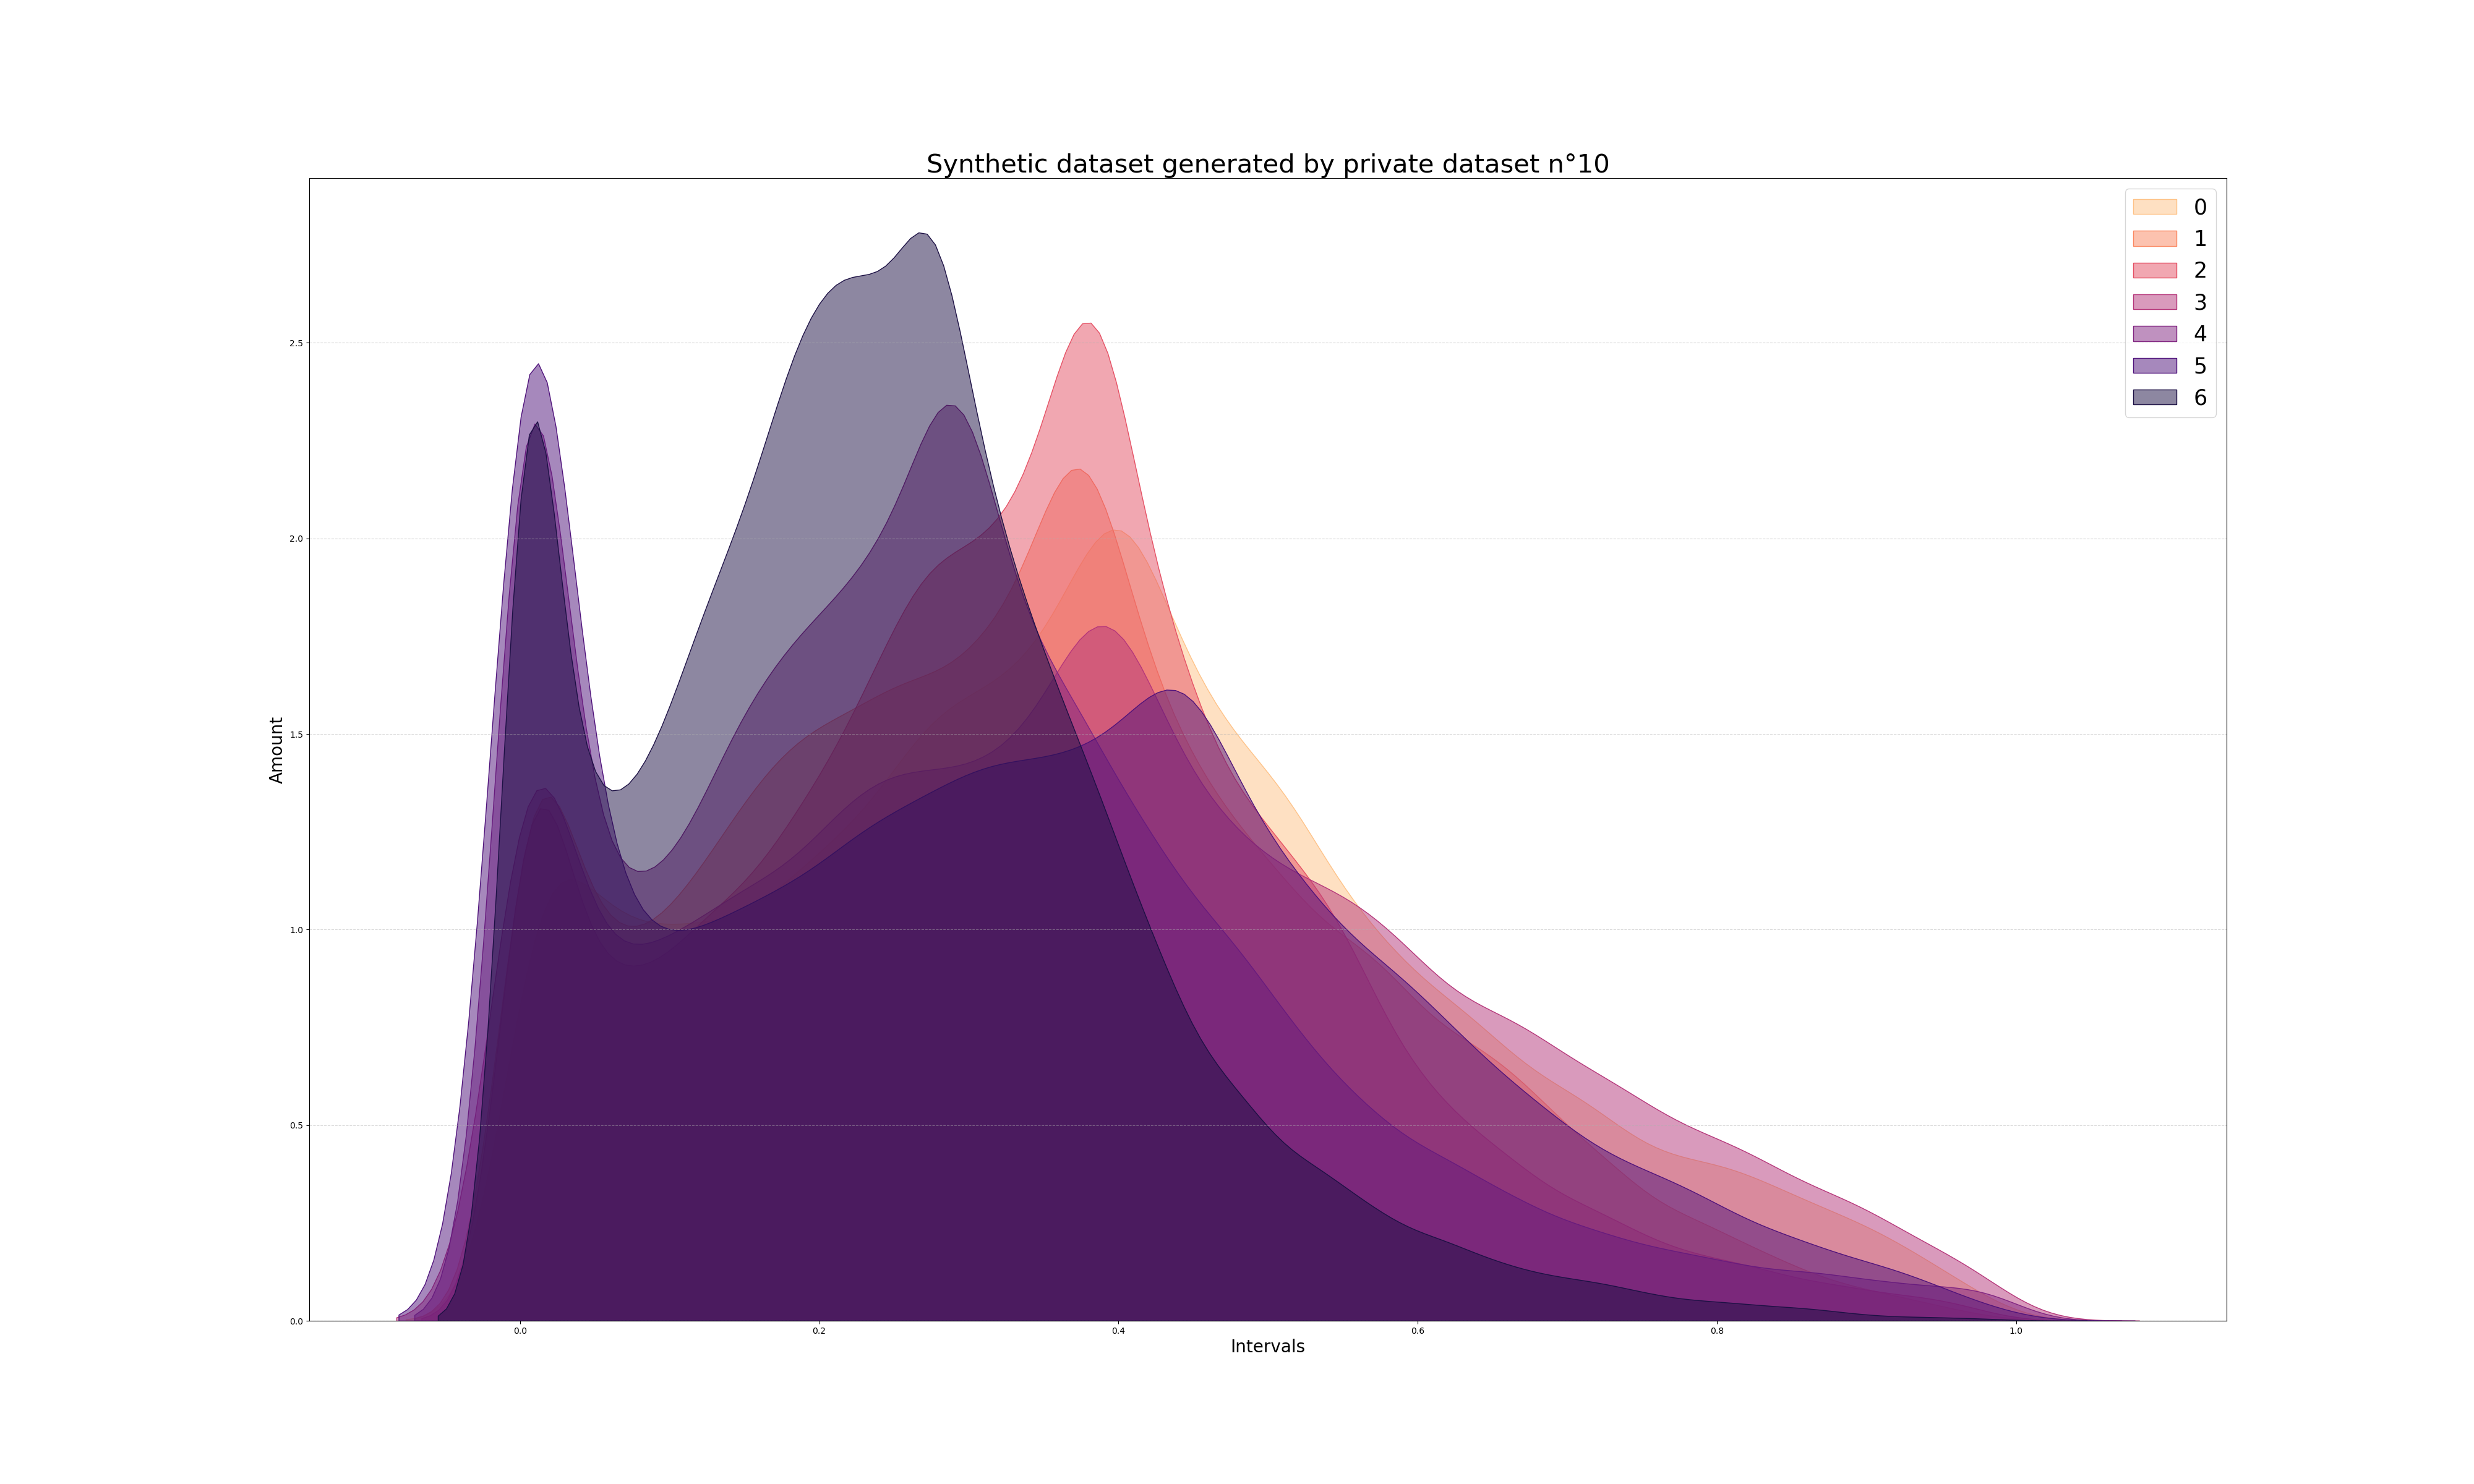
\includegraphics[width = 0.28\textwidth]{figures/Resultats/SyntheticDS/False Synthetics/Task 2/10}}}\qquad
            \subfloat[]{\fbox{
                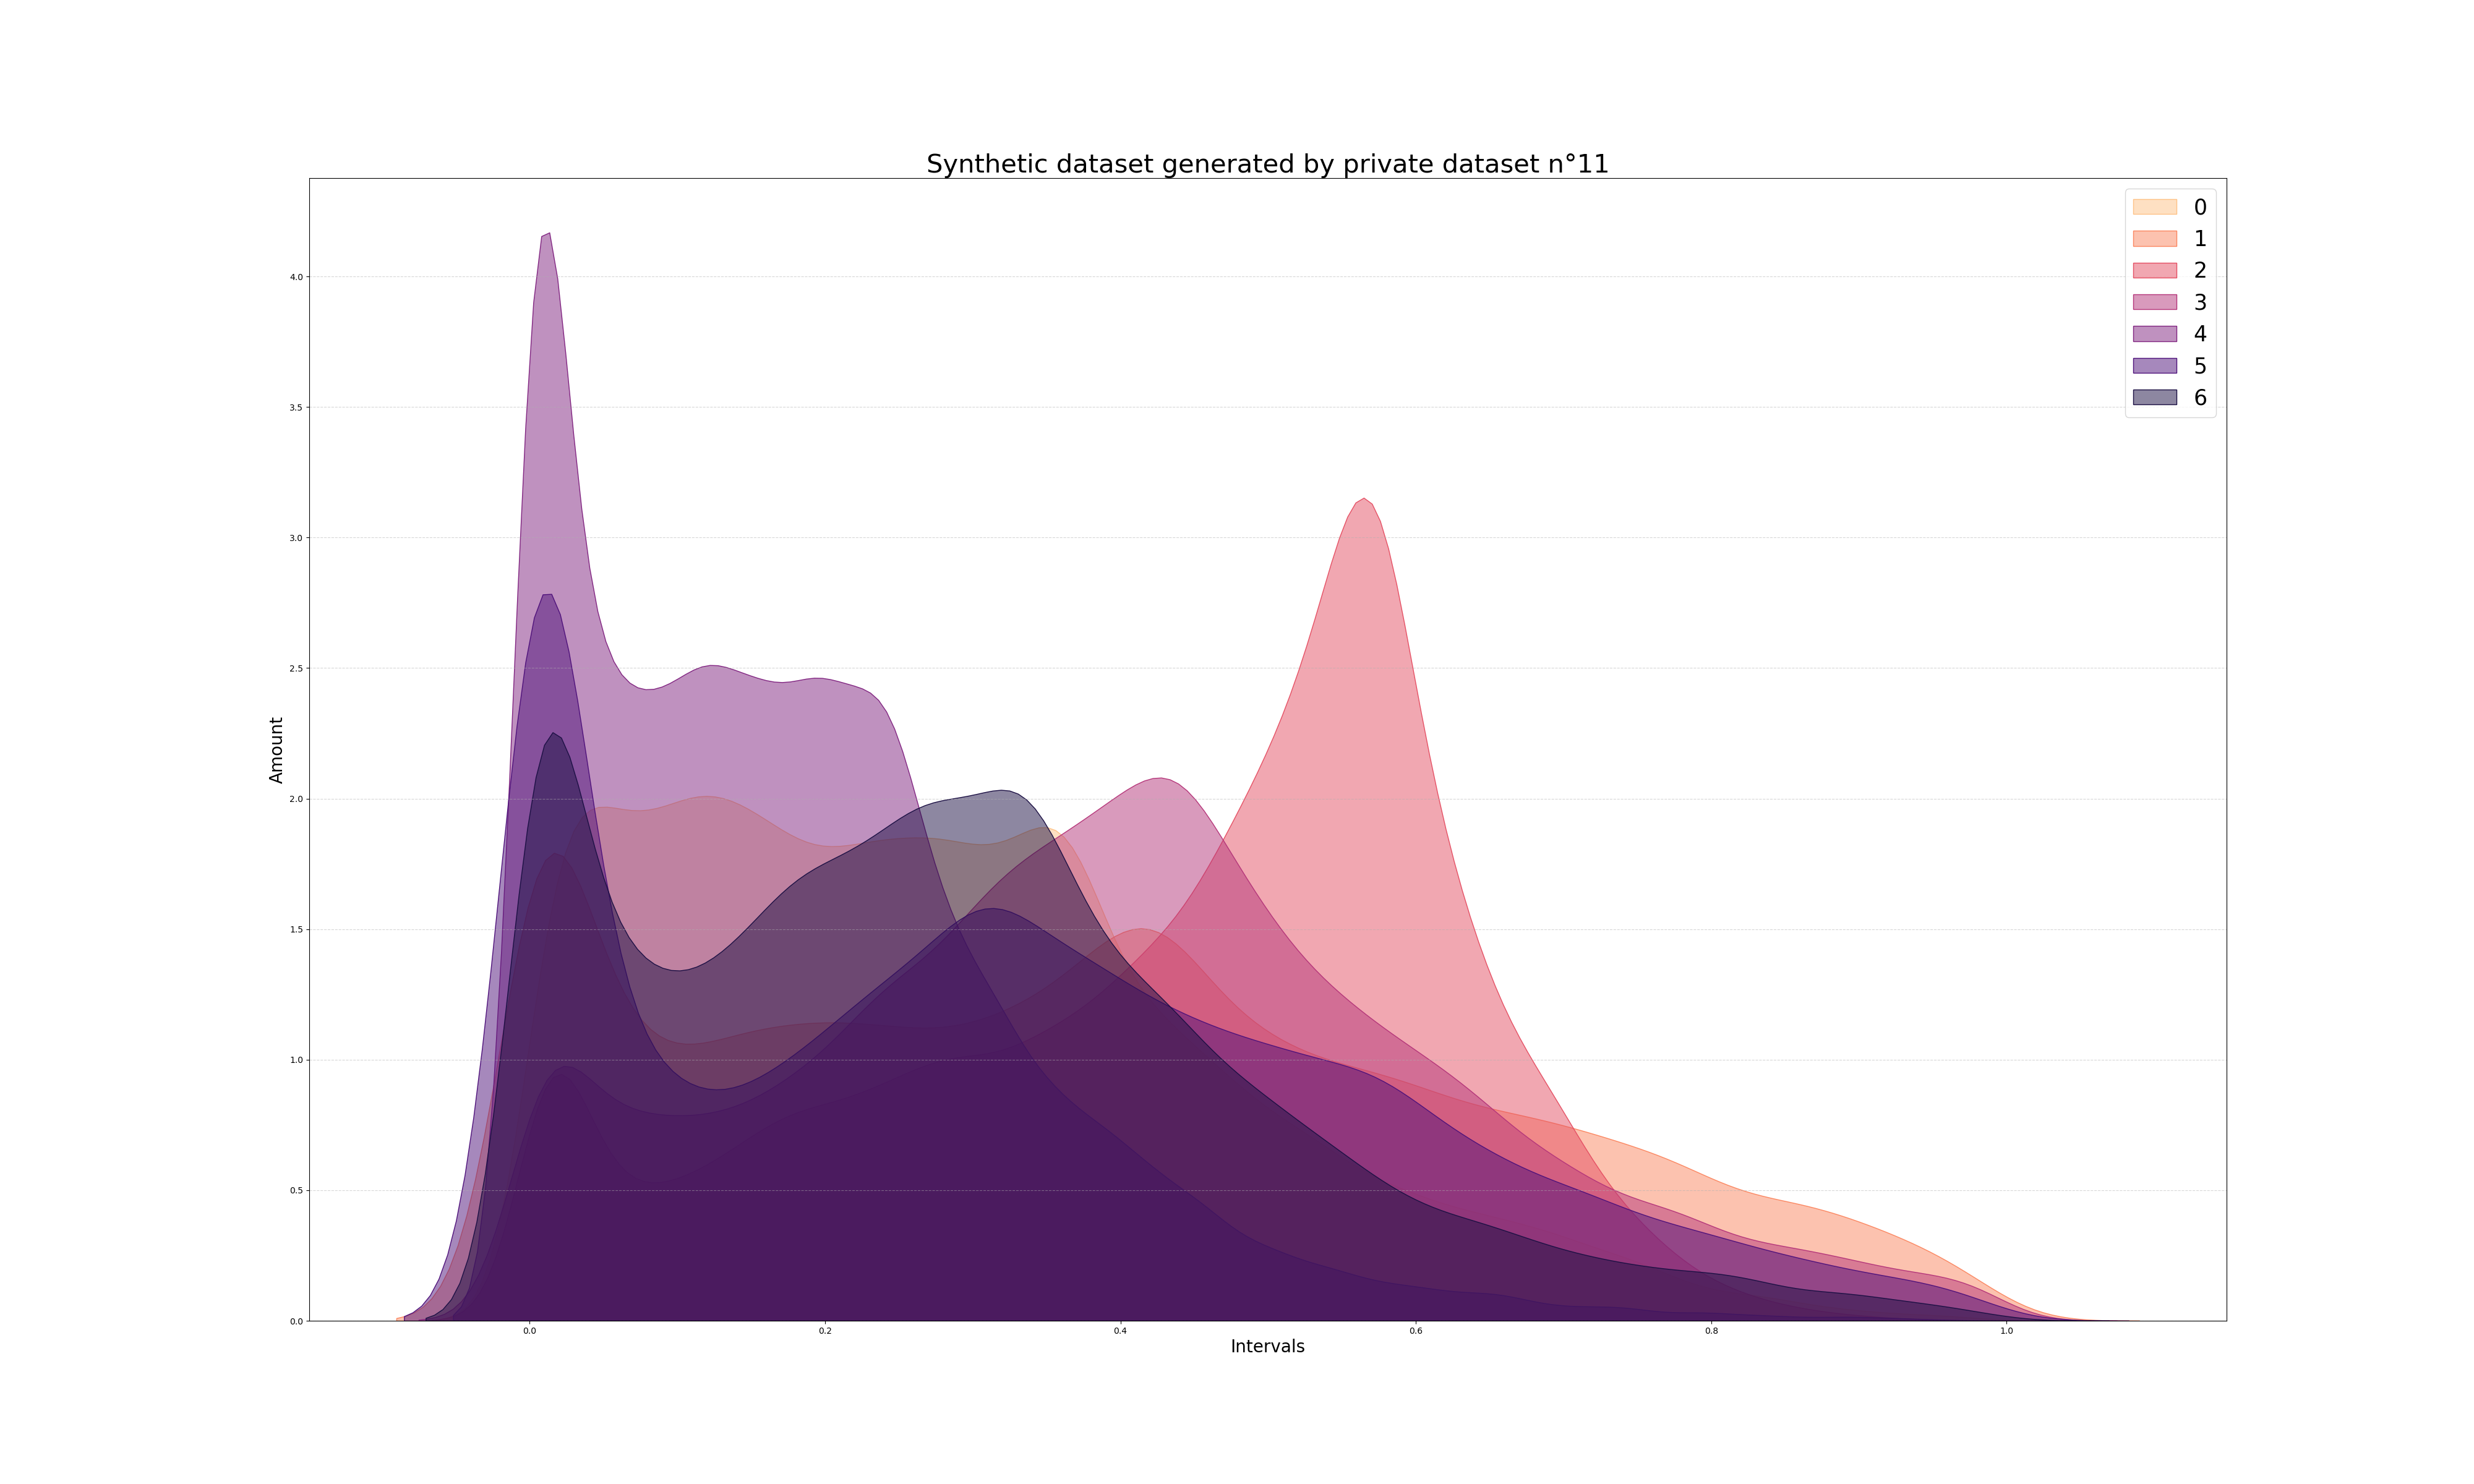
\includegraphics[width = 0.28\textwidth]{figures/Resultats/SyntheticDS/False Synthetics/Task 2/11}}}\qquad
            \subfloat[]{\fbox{
                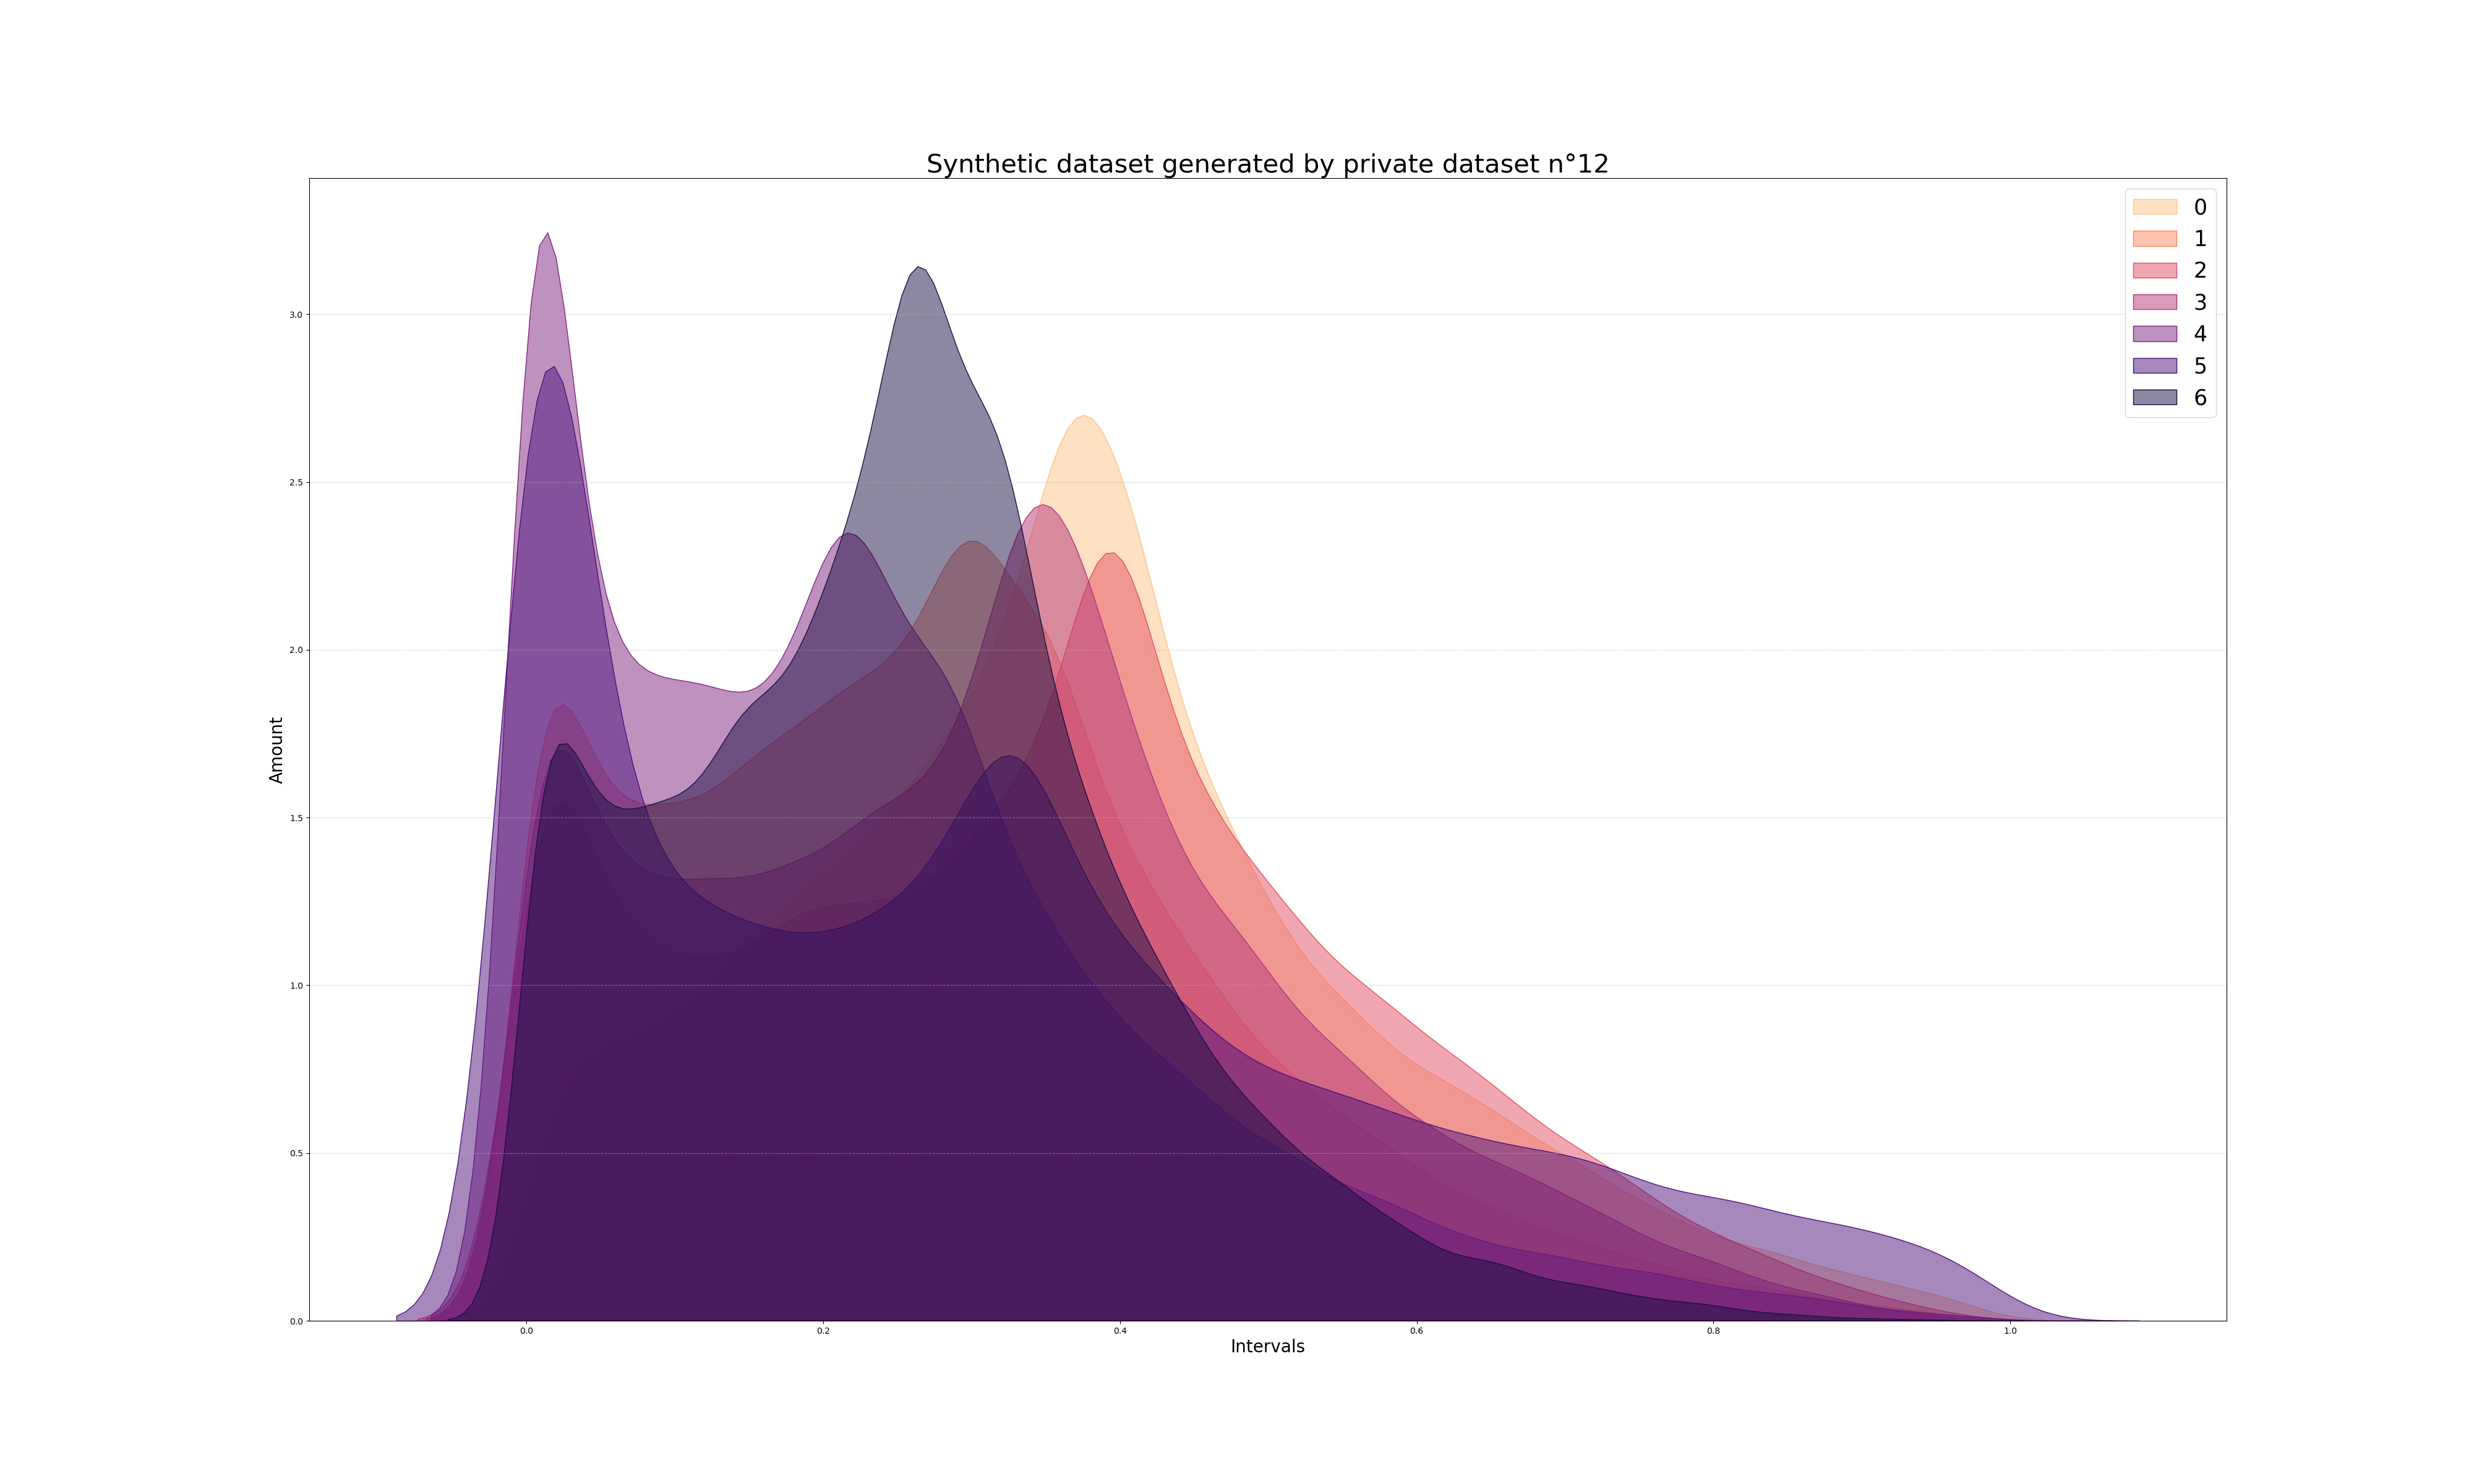
\includegraphics[width = 0.28\textwidth]{figures/Resultats/SyntheticDS/False Synthetics/Task 2/12}}}\qquad
            \subfloat[]{\fbox{
                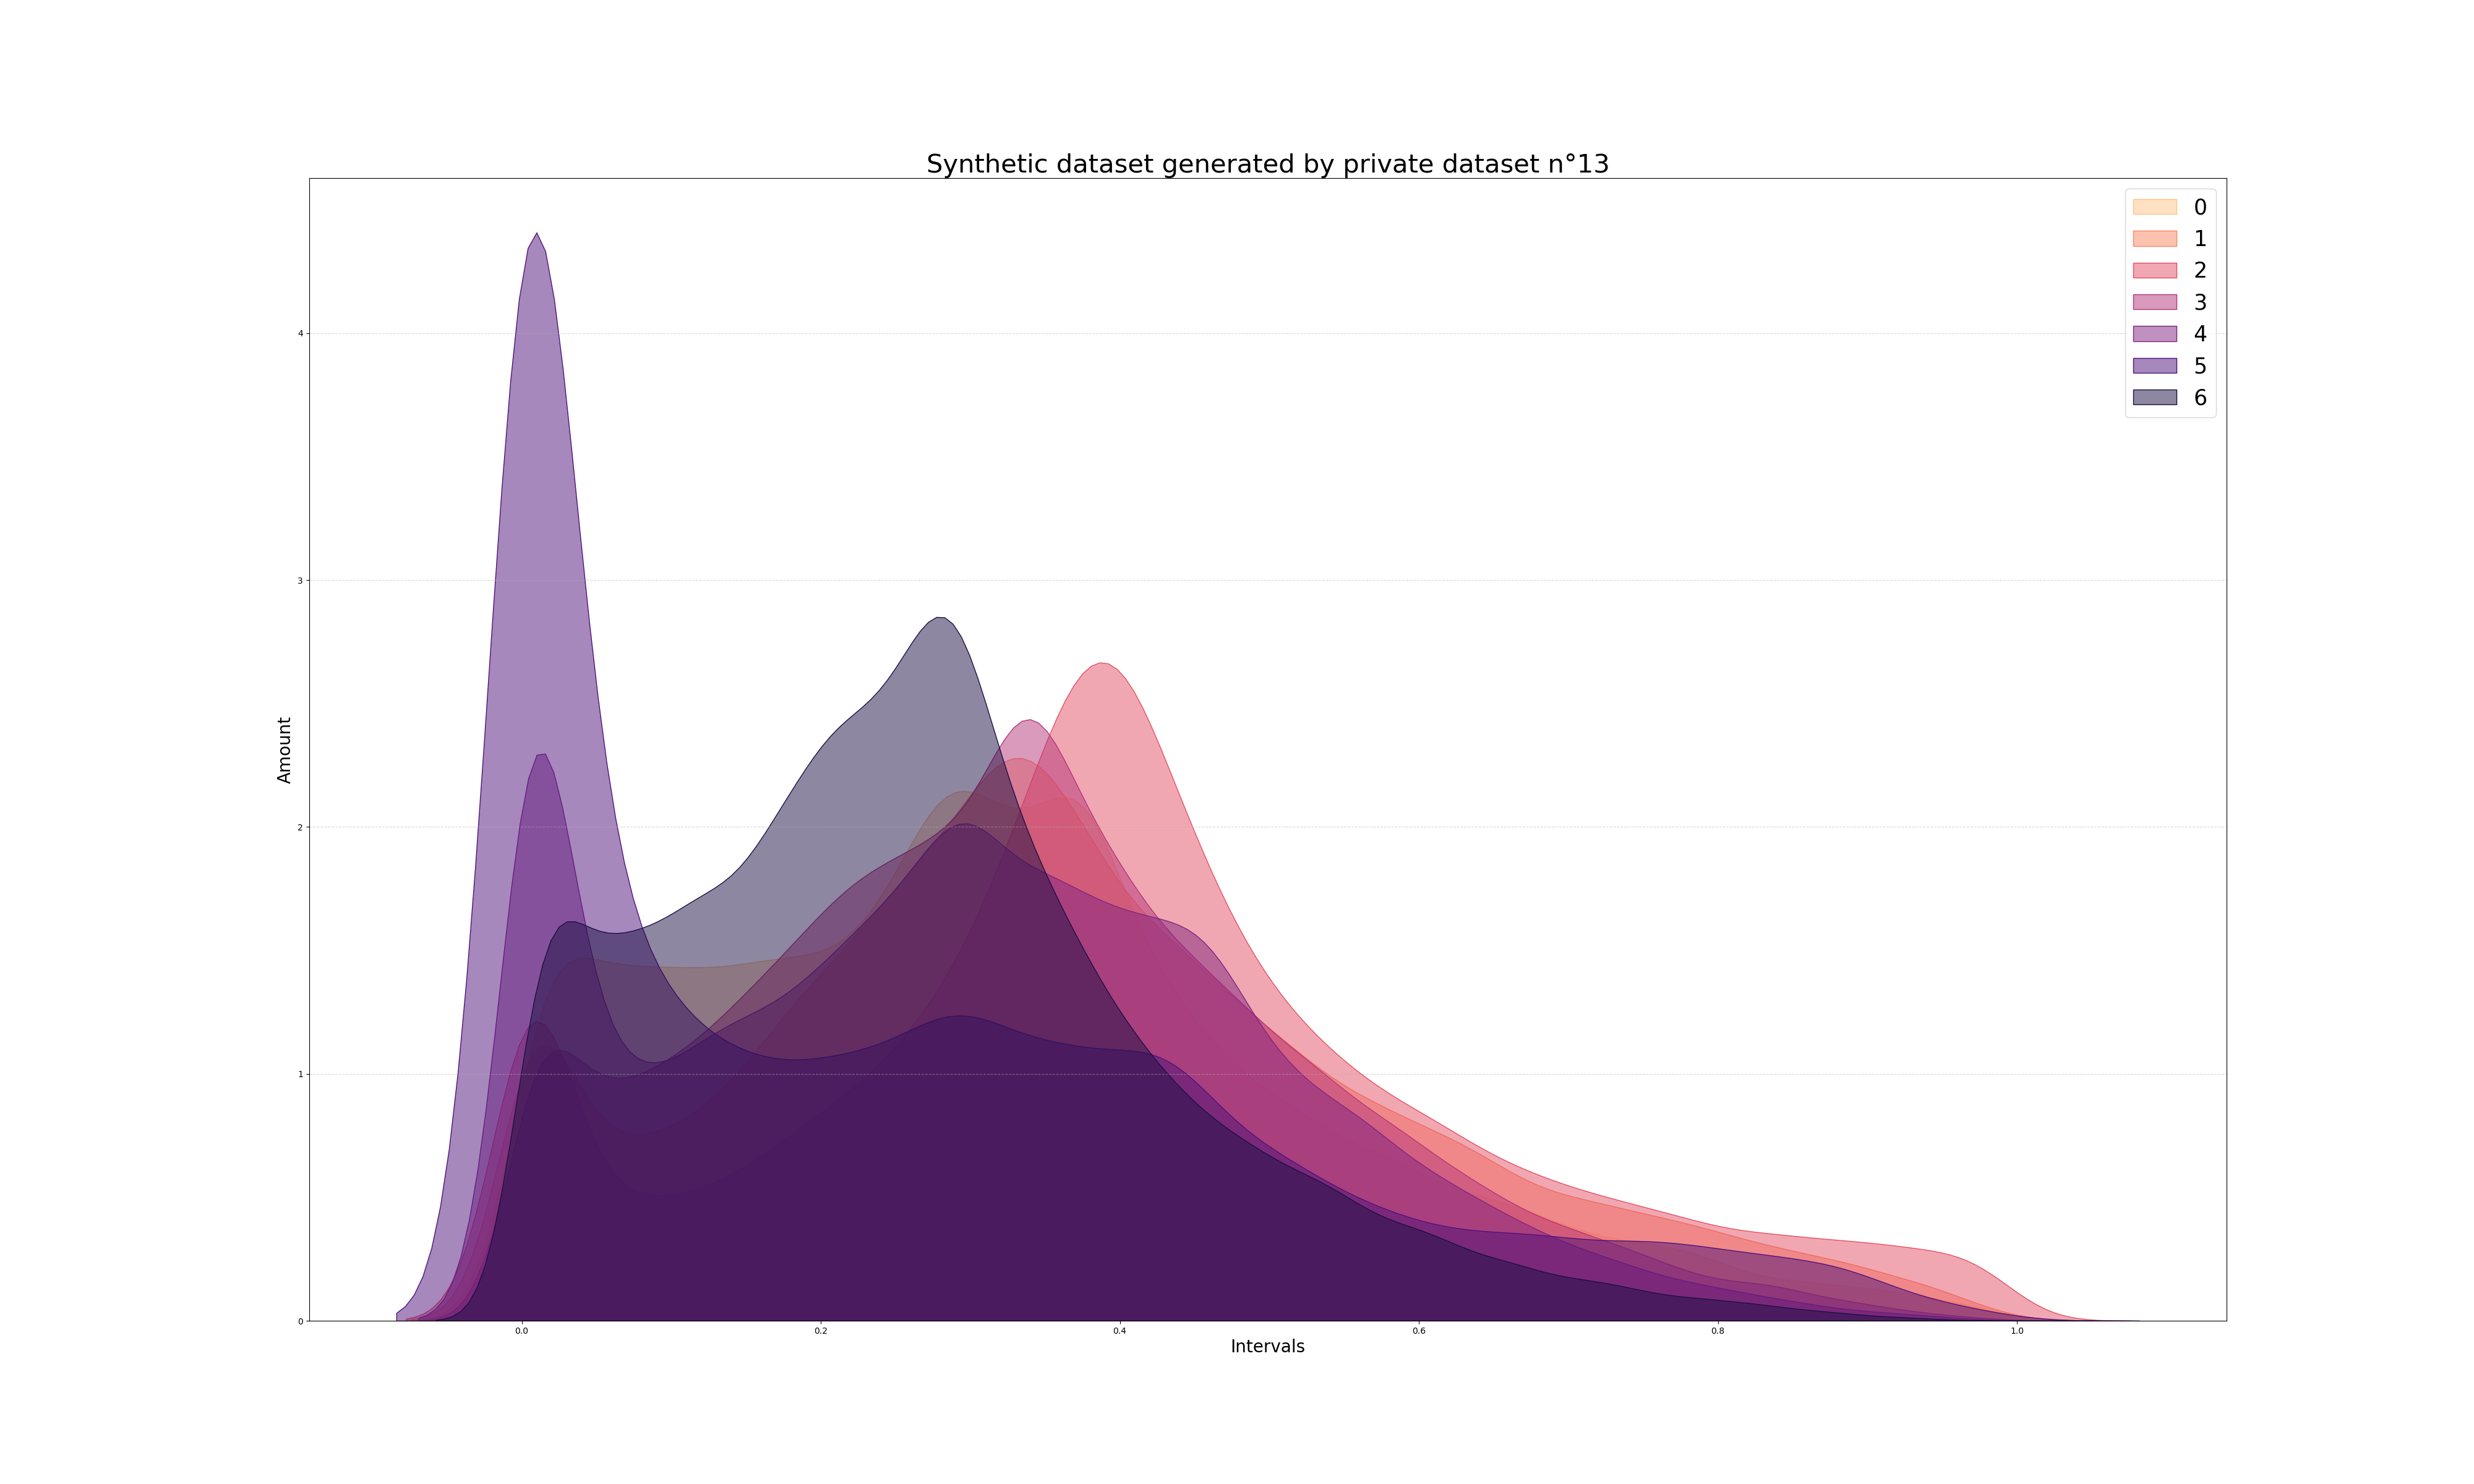
\includegraphics[width = 0.28\textwidth]{figures/Resultats/SyntheticDS/False Synthetics/Task 2/13}}}\qquad
            \subfloat[]{\fbox{
                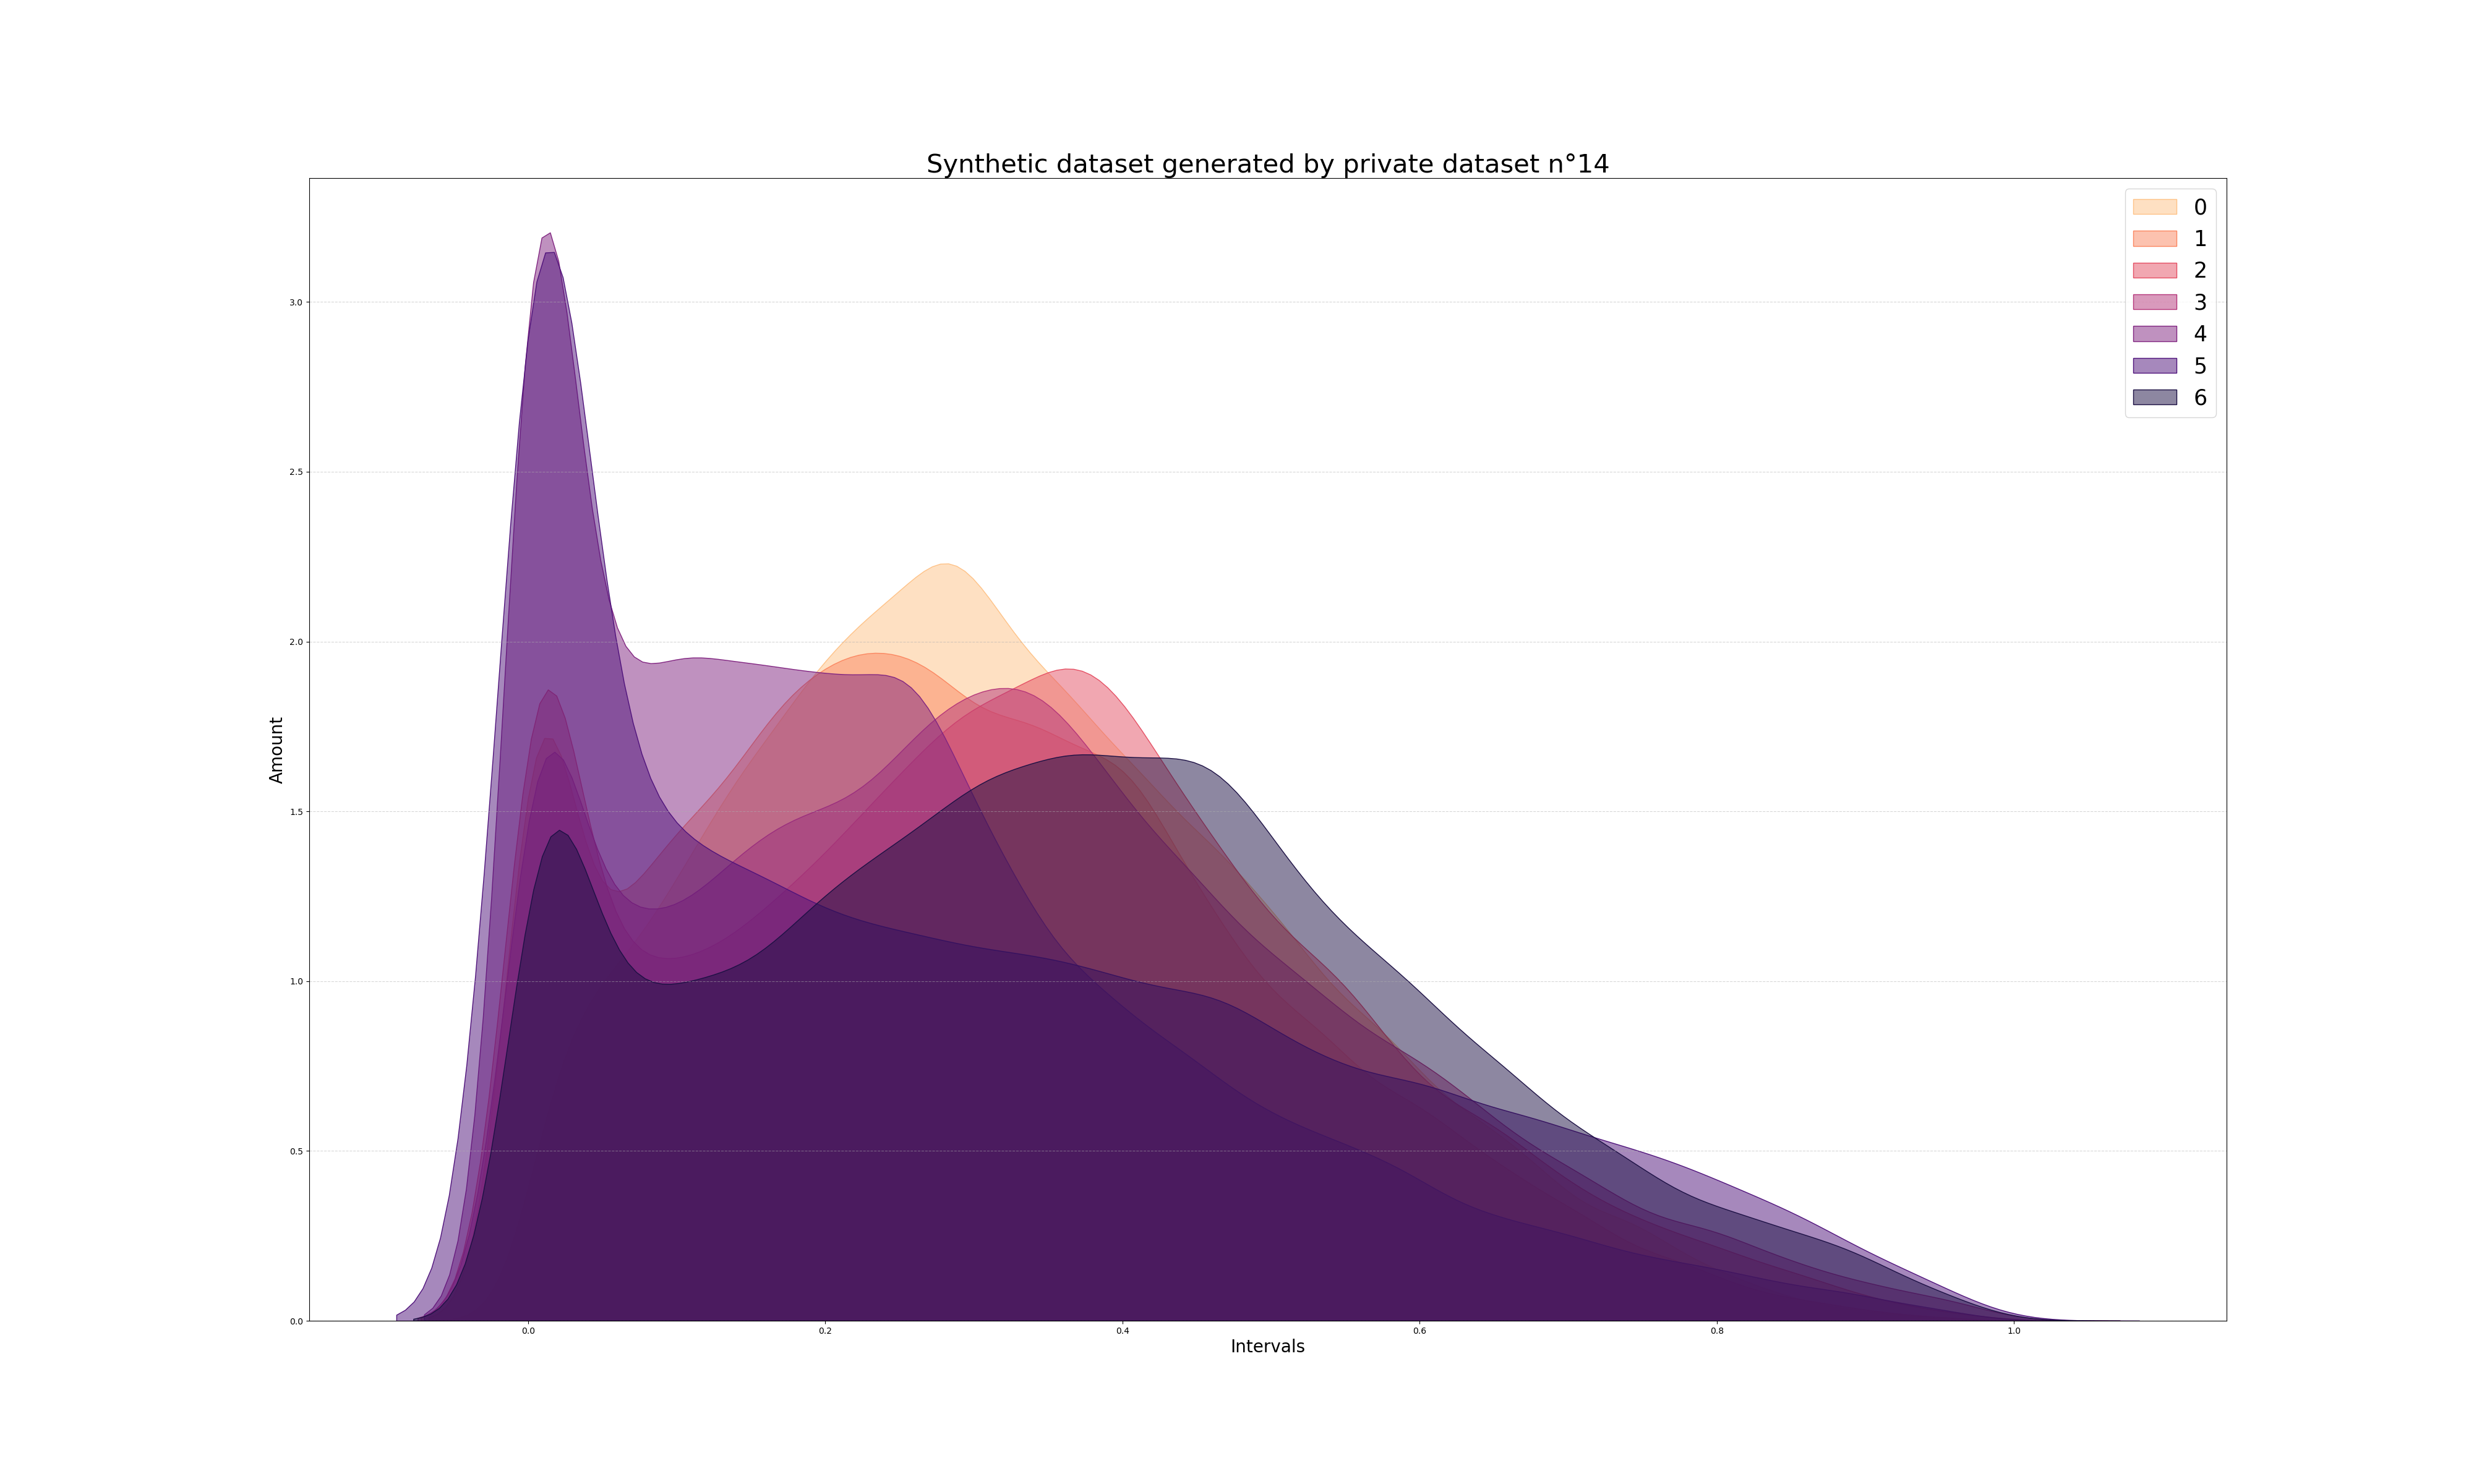
\includegraphics[width = 0.28\textwidth]{figures/Resultats/SyntheticDS/False Synthetics/Task 2/14}}}\qquad
            \subfloat[]{\fbox{
                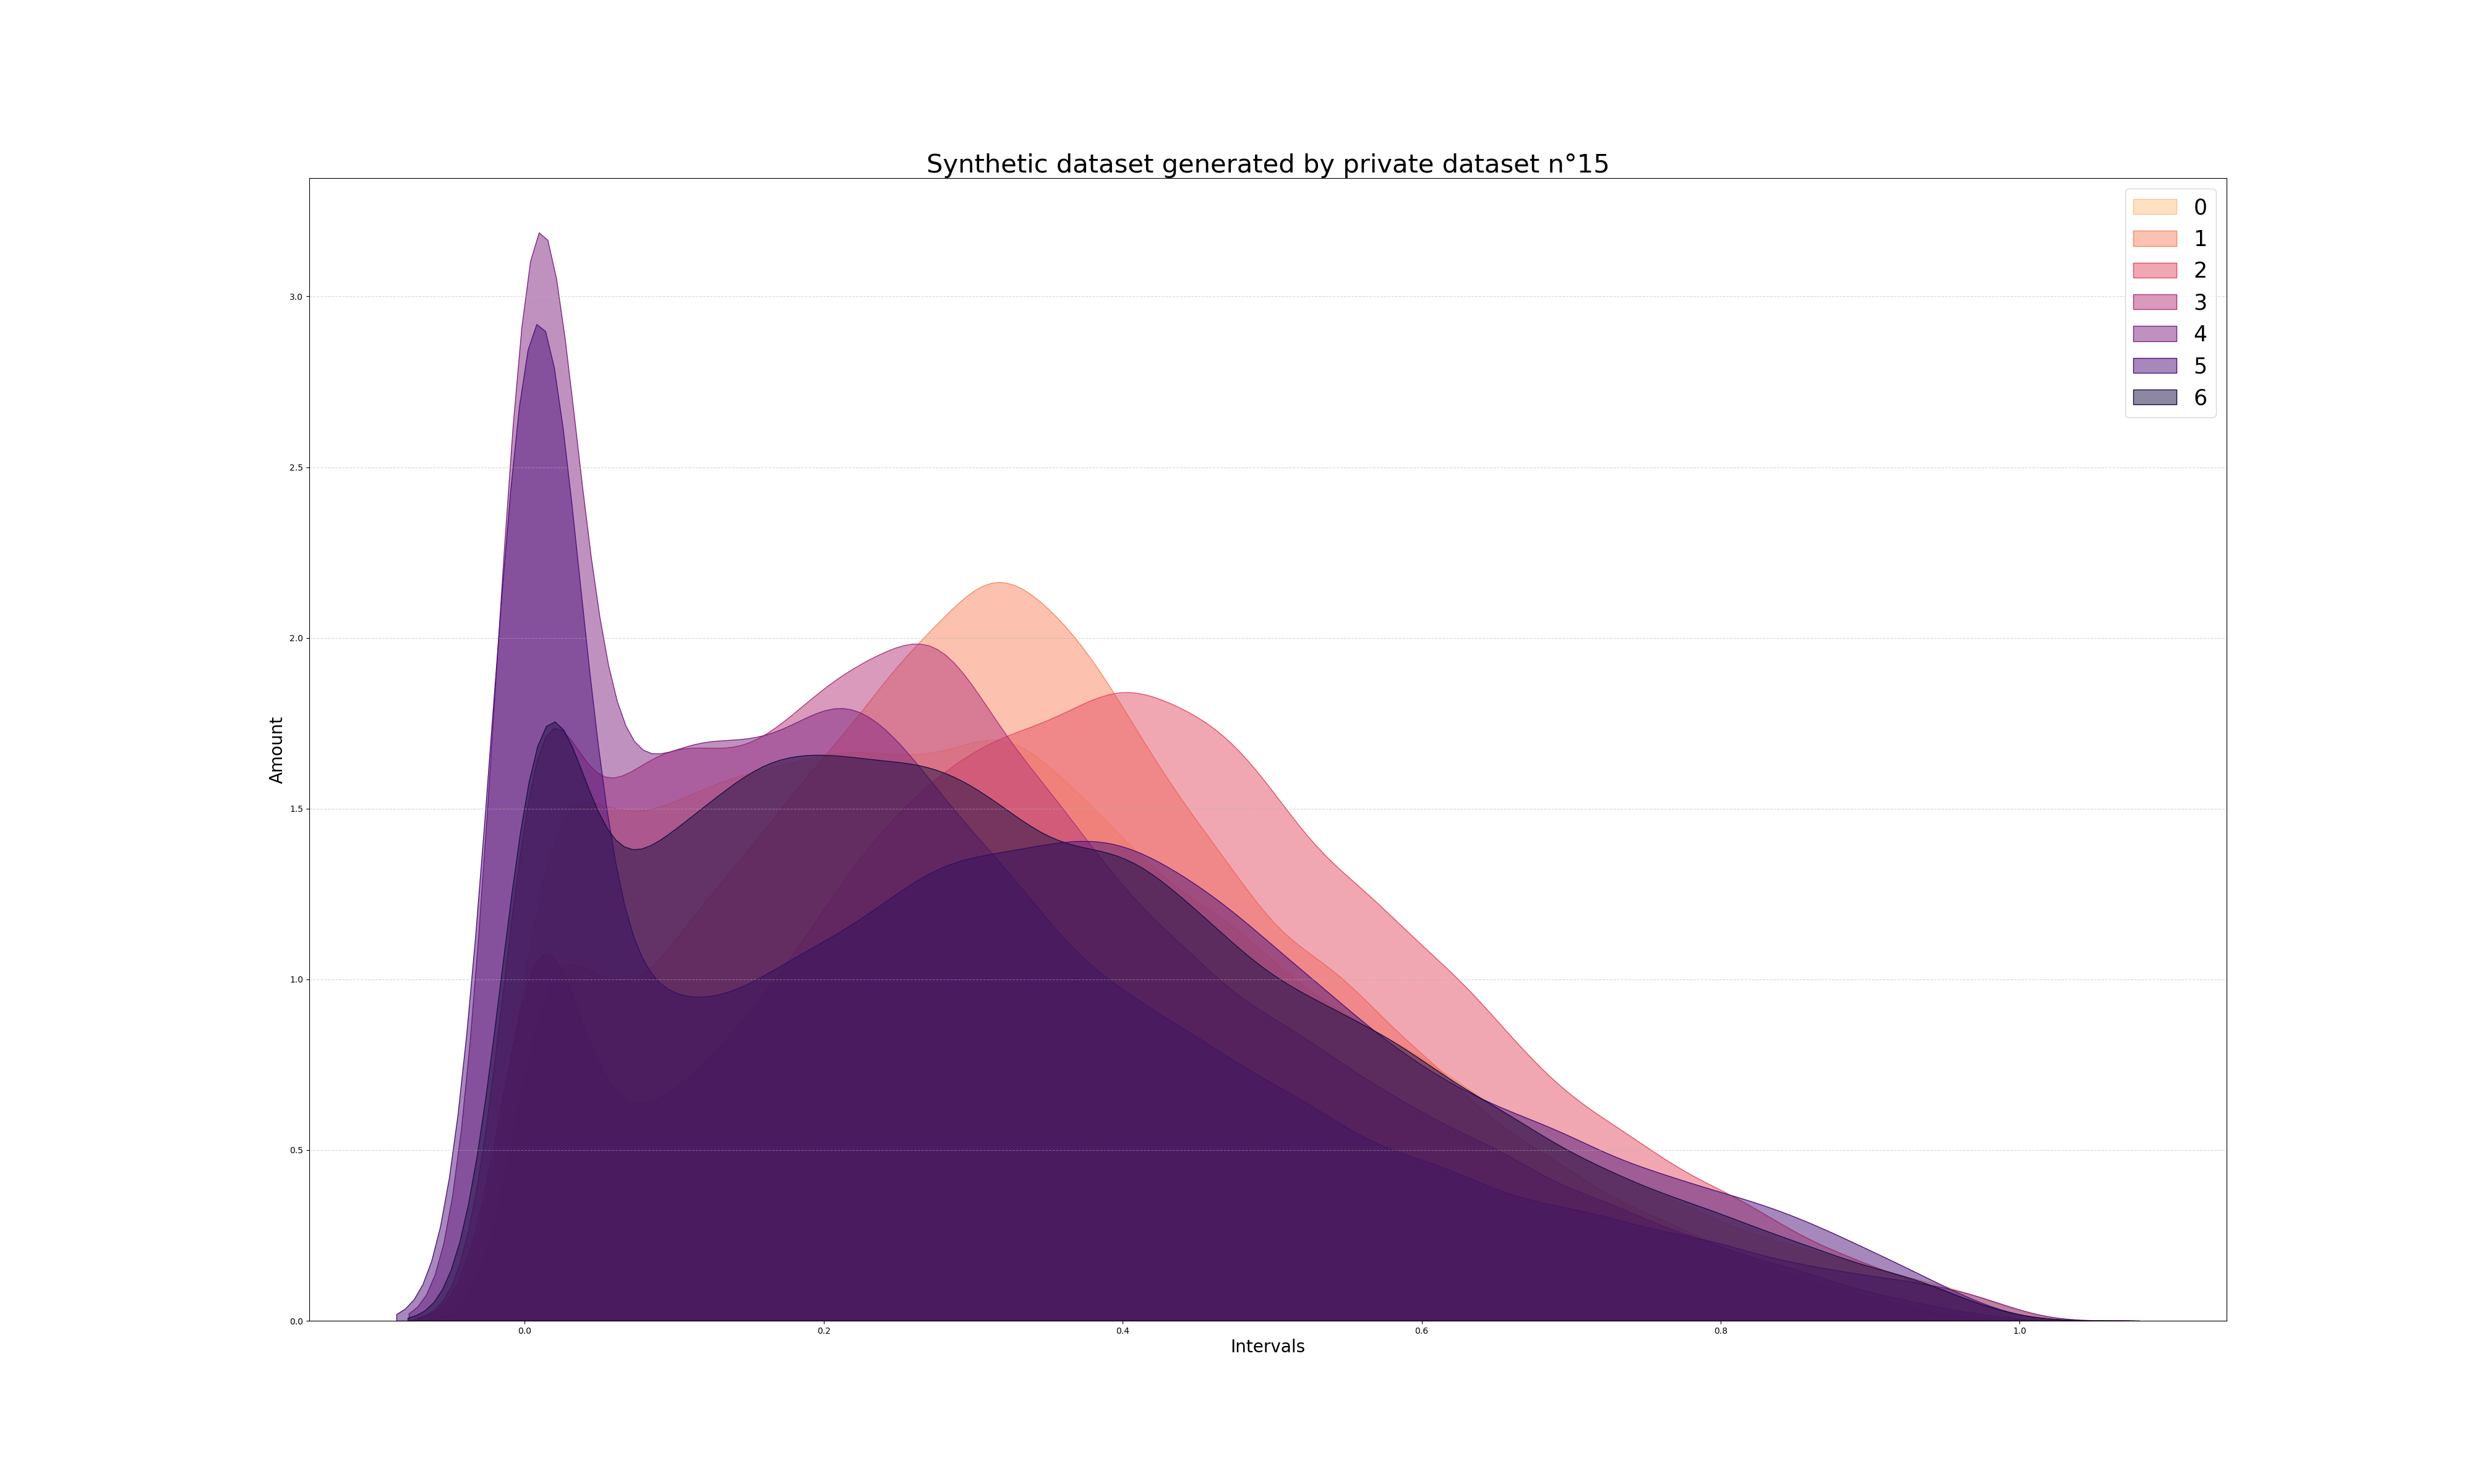
\includegraphics[width = 0.28\textwidth]{figures/Resultats/SyntheticDS/False Synthetics/Task 2/15}}}\qquad
            \caption{Distribution des datasets synthétiques générés par les datasets privés - $\mathfrak H\left( \mathbb{S}'_{Synth_{i_{T_{2}}}}\right) \Bigm \lvert \left(E_{T_2, \overline C, l_{30}}\right)$}
            \label{H15Synth}
        \end{figure}

        \label{divNonTrivial}\begin{tcolorbox}[colback=linkborder_Color!5!white,colframe=
linkborder_Color!75!
black]
            Ce changement d'échelle permet d'augmenter les performances du classifieur
            \textit{(voir \ref{classif})} sans pour autant se soucier davantage de la qualité des
            données fournies. Une approche naïve envisagée en début de projet était de comparer à
            l'oeil les distributions, et d'exclure arbitrairement les $\mathbb S'_{priv_i}$ dont
            l'allure paraissait impropre à l'inclusion dans l'entraînement du classifieur. Une
            telle approche engendre de moins bons résultats. Ce problème s'éclaircit quand on
            visualise la divergence \footnote{voir section suivante pour le choix de la métrique} des
            données utilisées avec $\mathbb S_{synth_{T_2}}$ : en réalité tous les datasets sont
            relativement éloignés de celui que l'on cherche à reproduire ! Il faut donc affiner le
            critère de sélection si l'on veut discriminer certains d'entre eux.
        \end{tcolorbox}

            \begin{figure}[H]
                \centering
                \subfloat[]{\fbox{
                    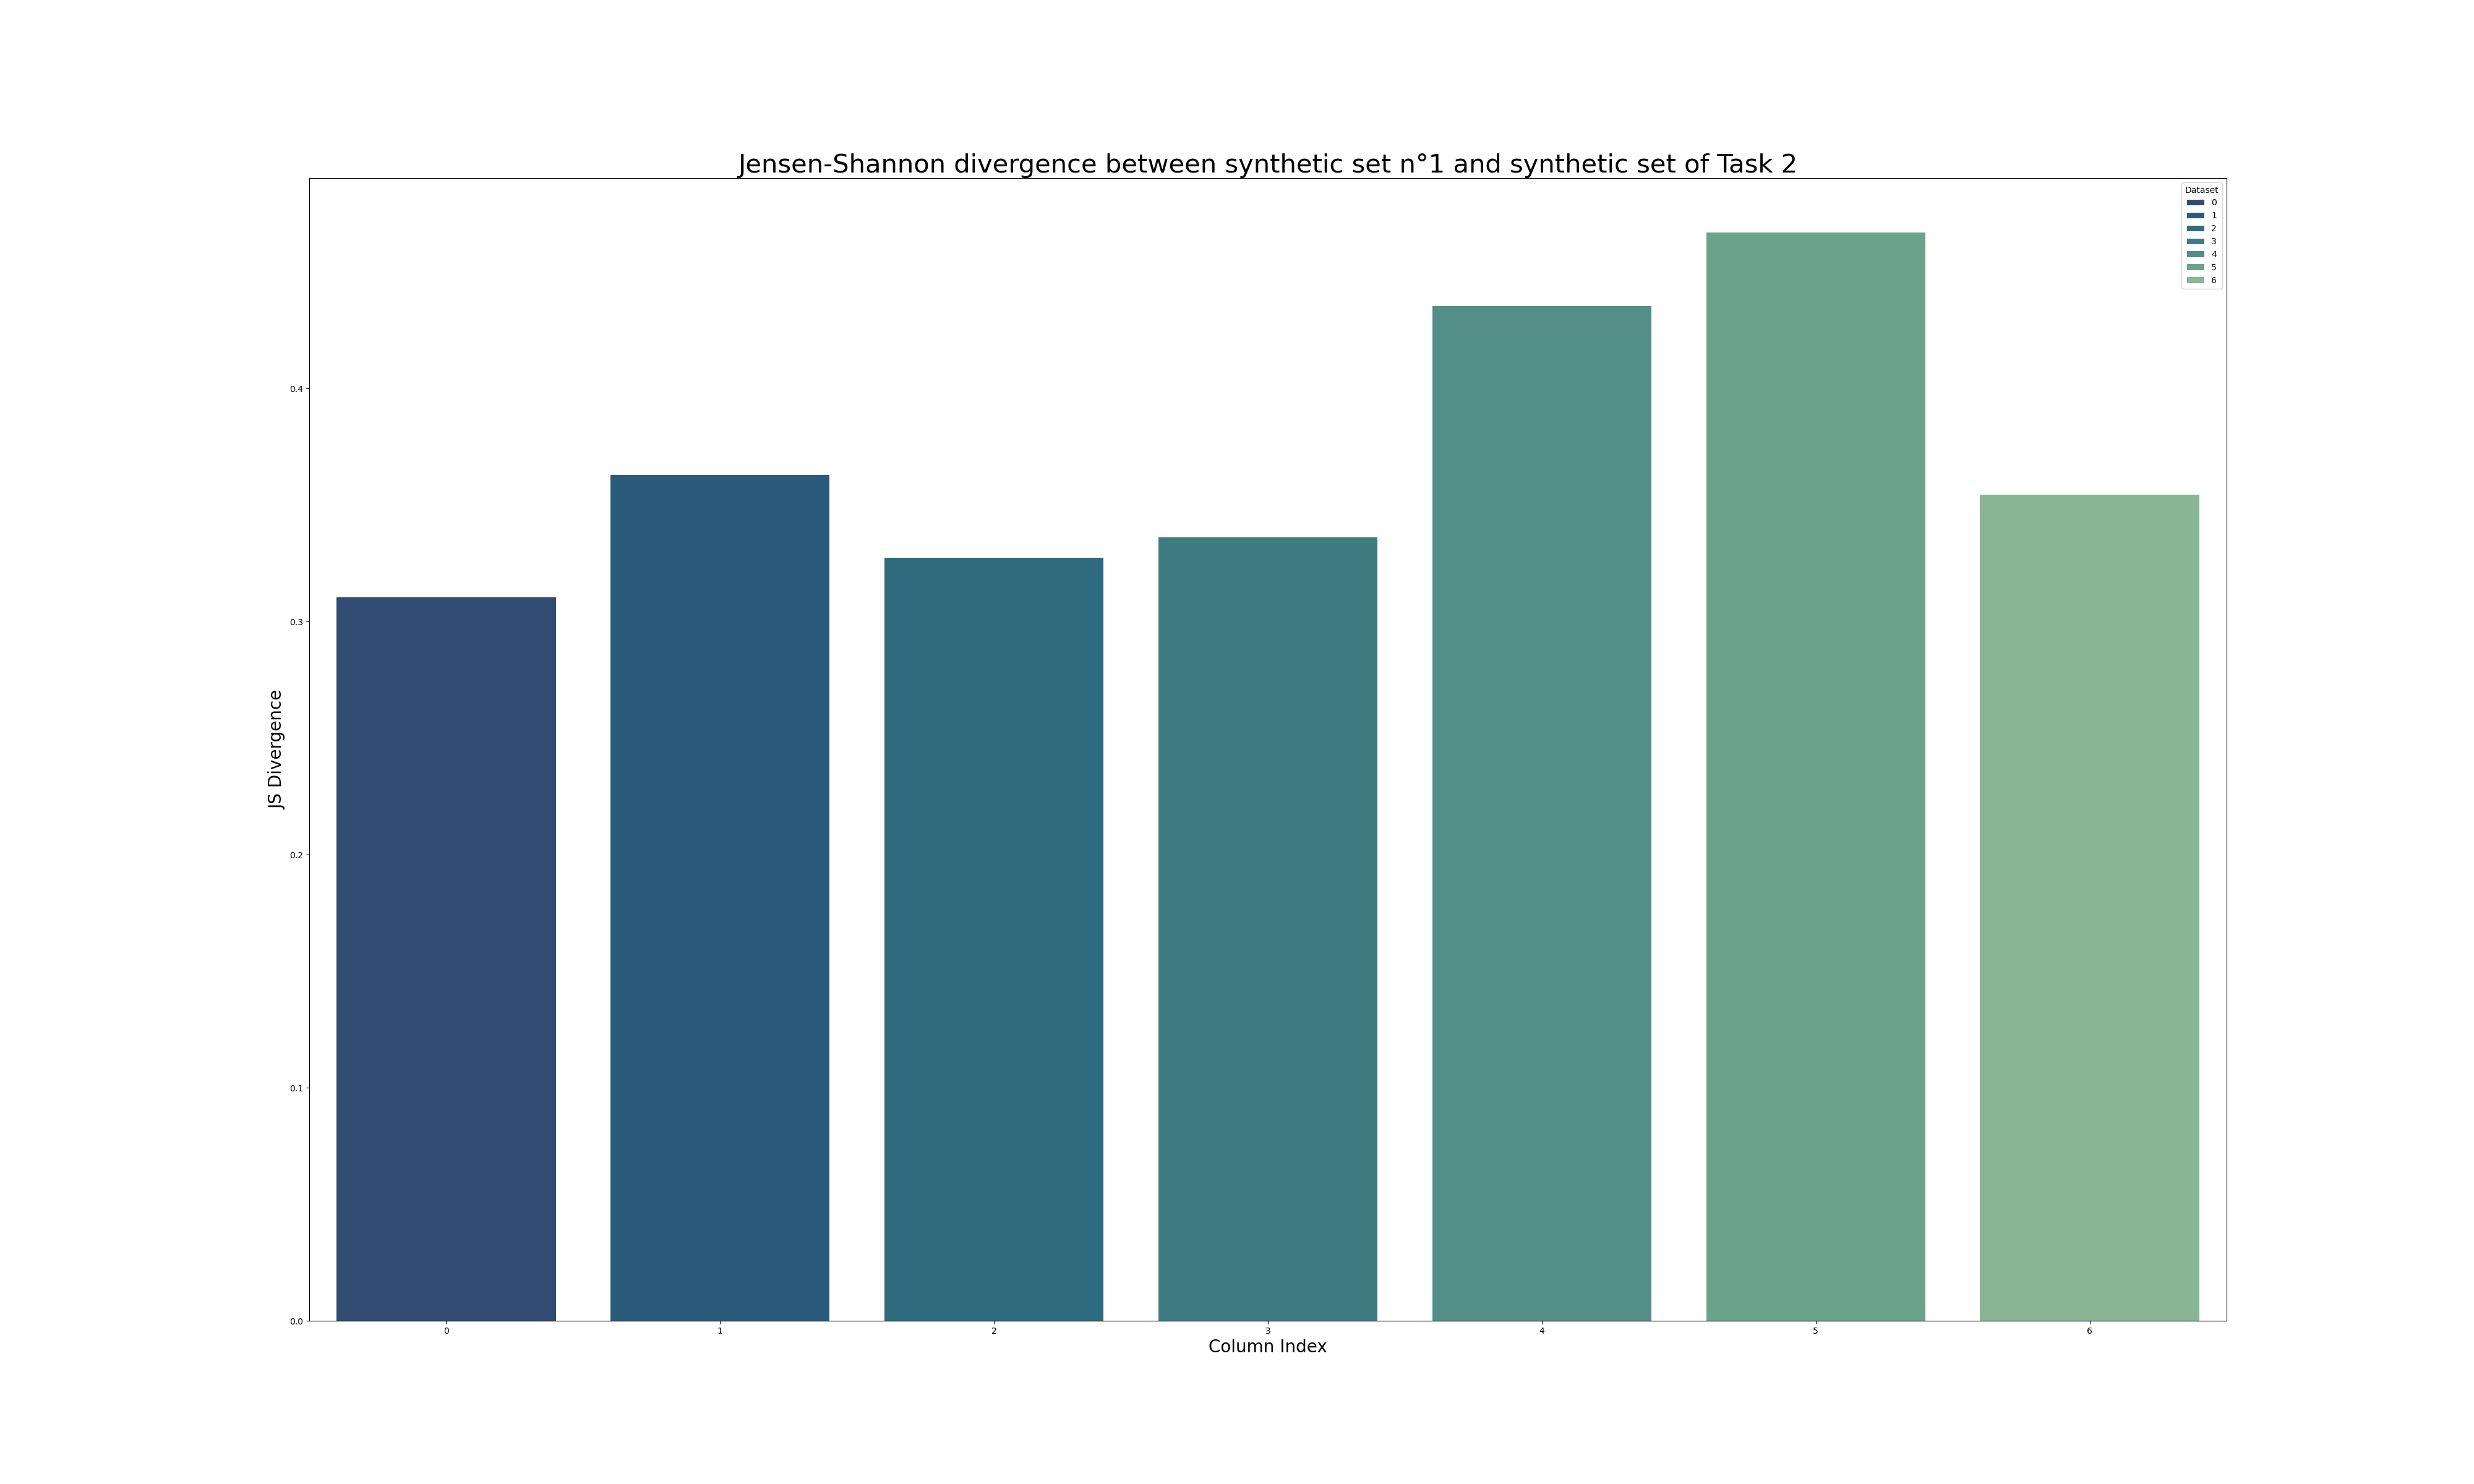
\includegraphics[width = 0.28\textwidth]{figures/Resultats/JSDivergences/1}}}\qquad
                \subfloat[]{\fbox{
                    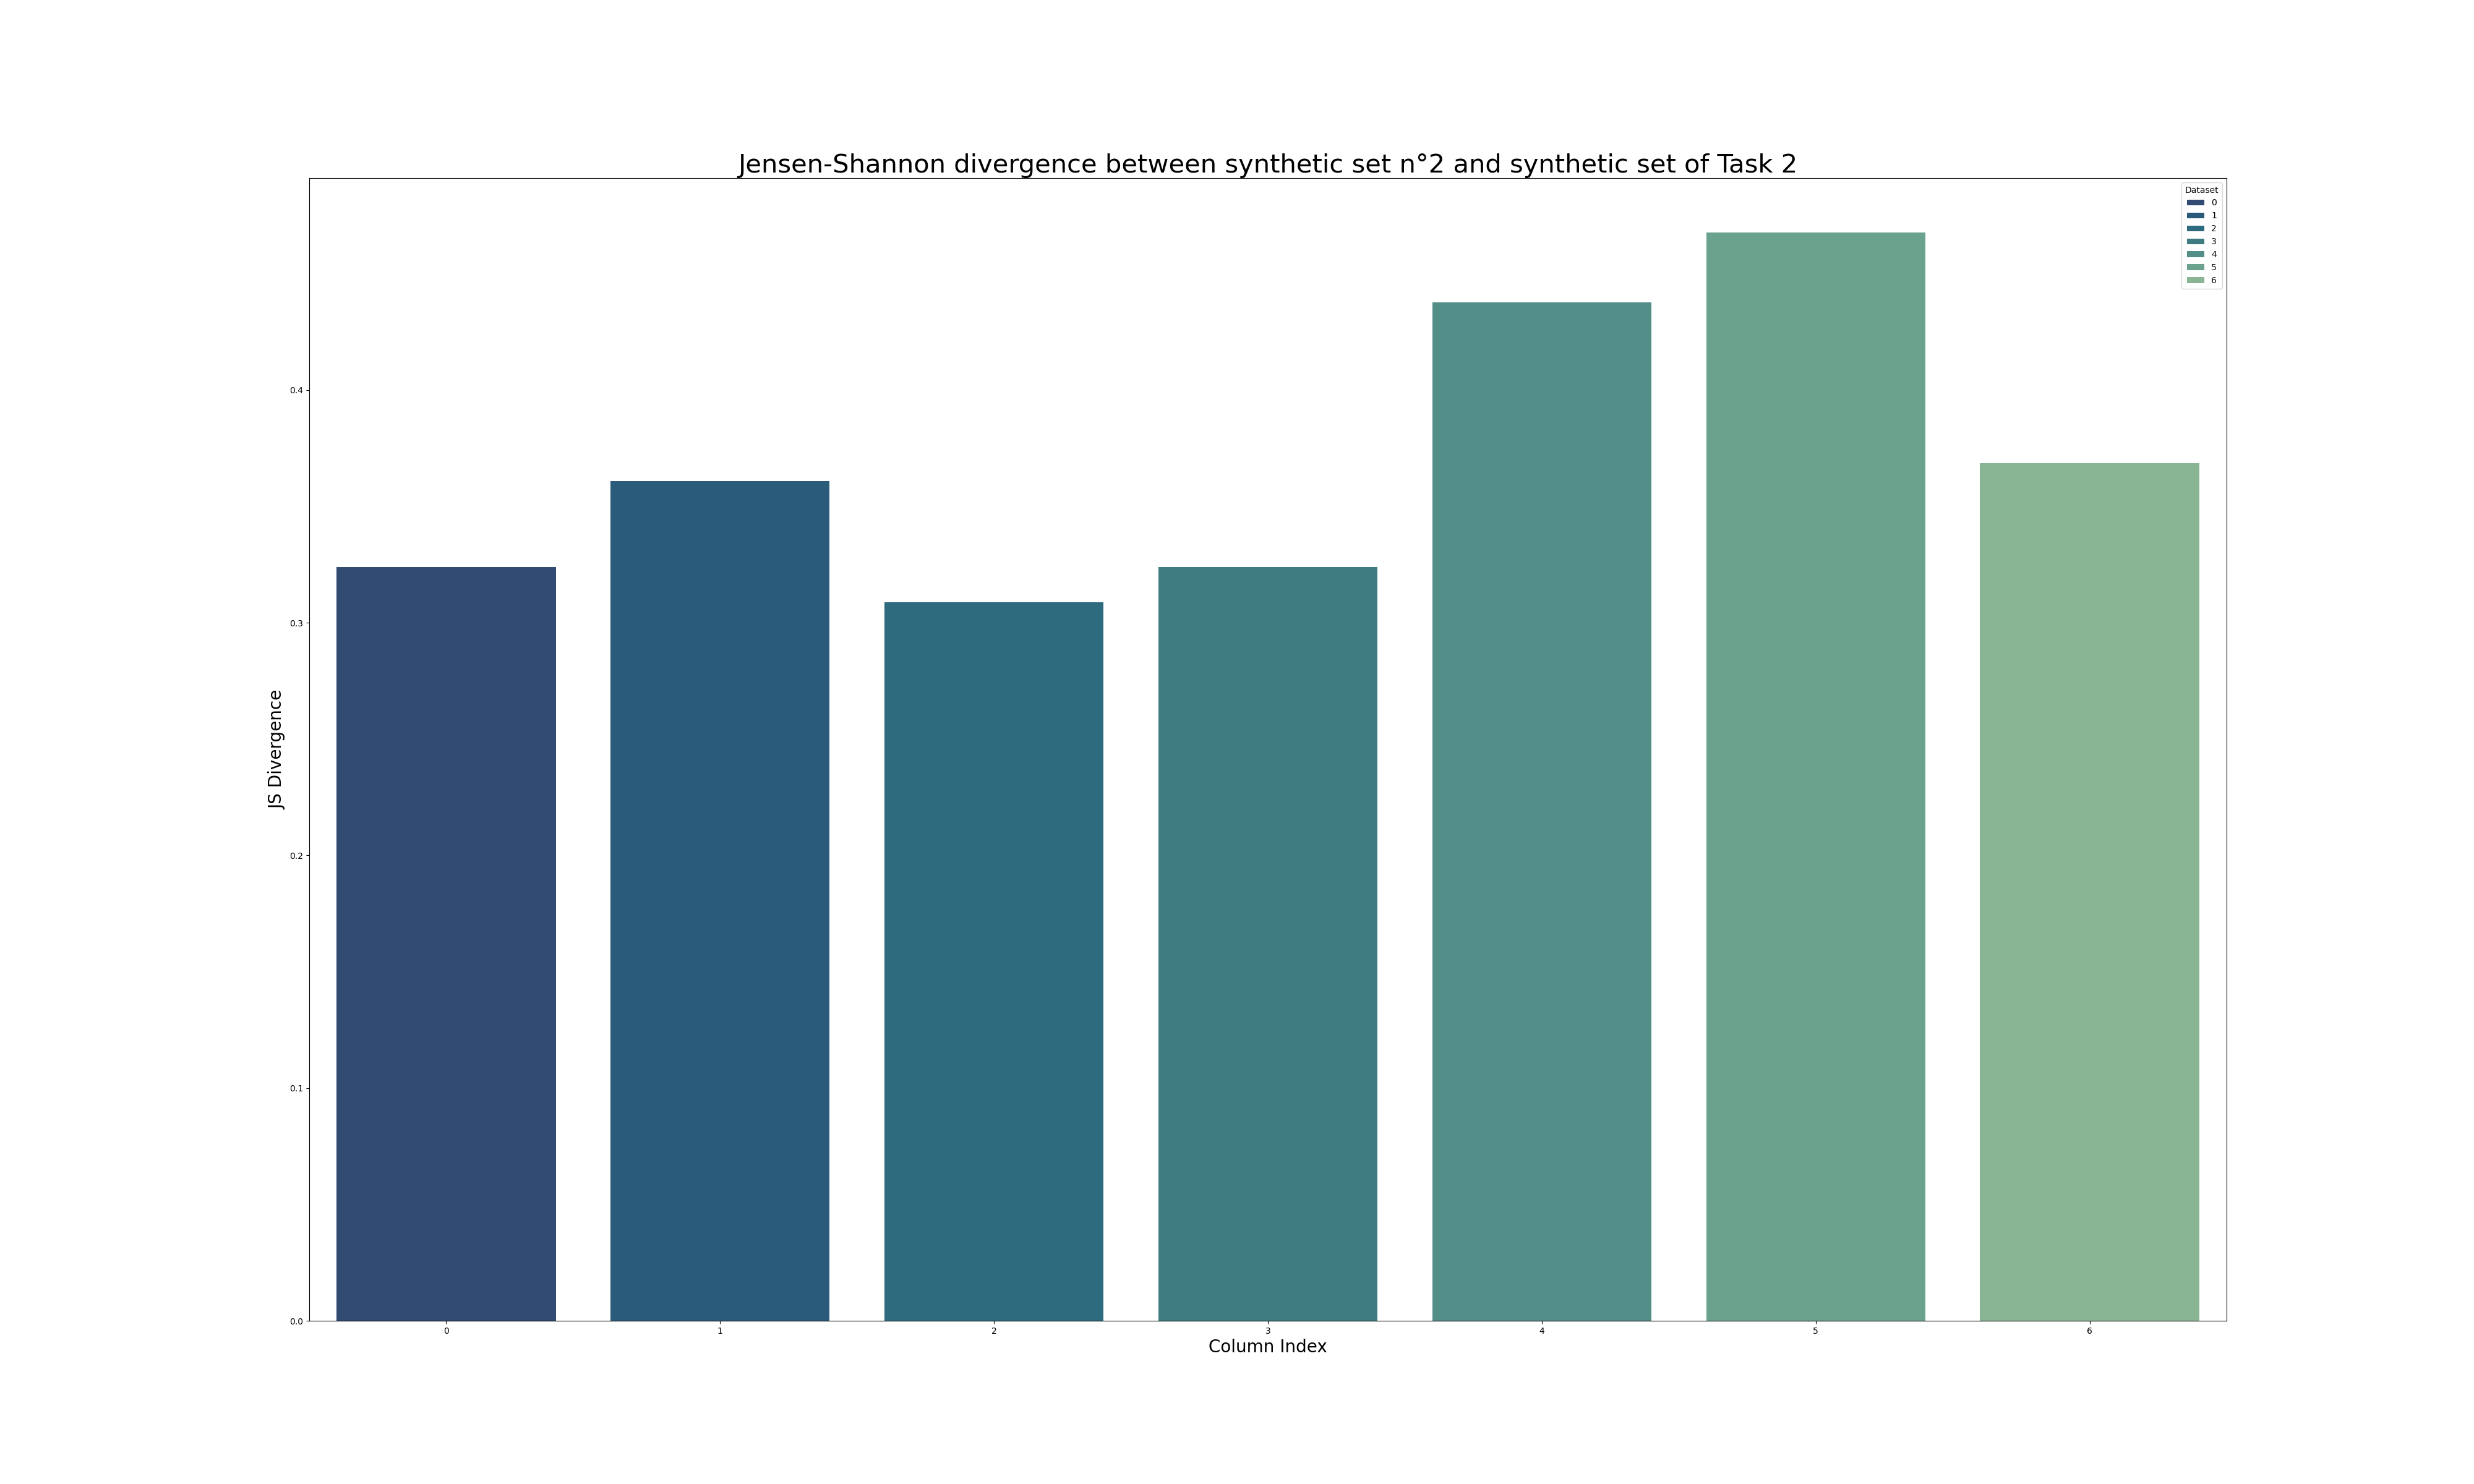
\includegraphics[width = 0.28\textwidth]{figures/Resultats/JSDivergences/2}}}\qquad
                \subfloat[]{\fbox{
                    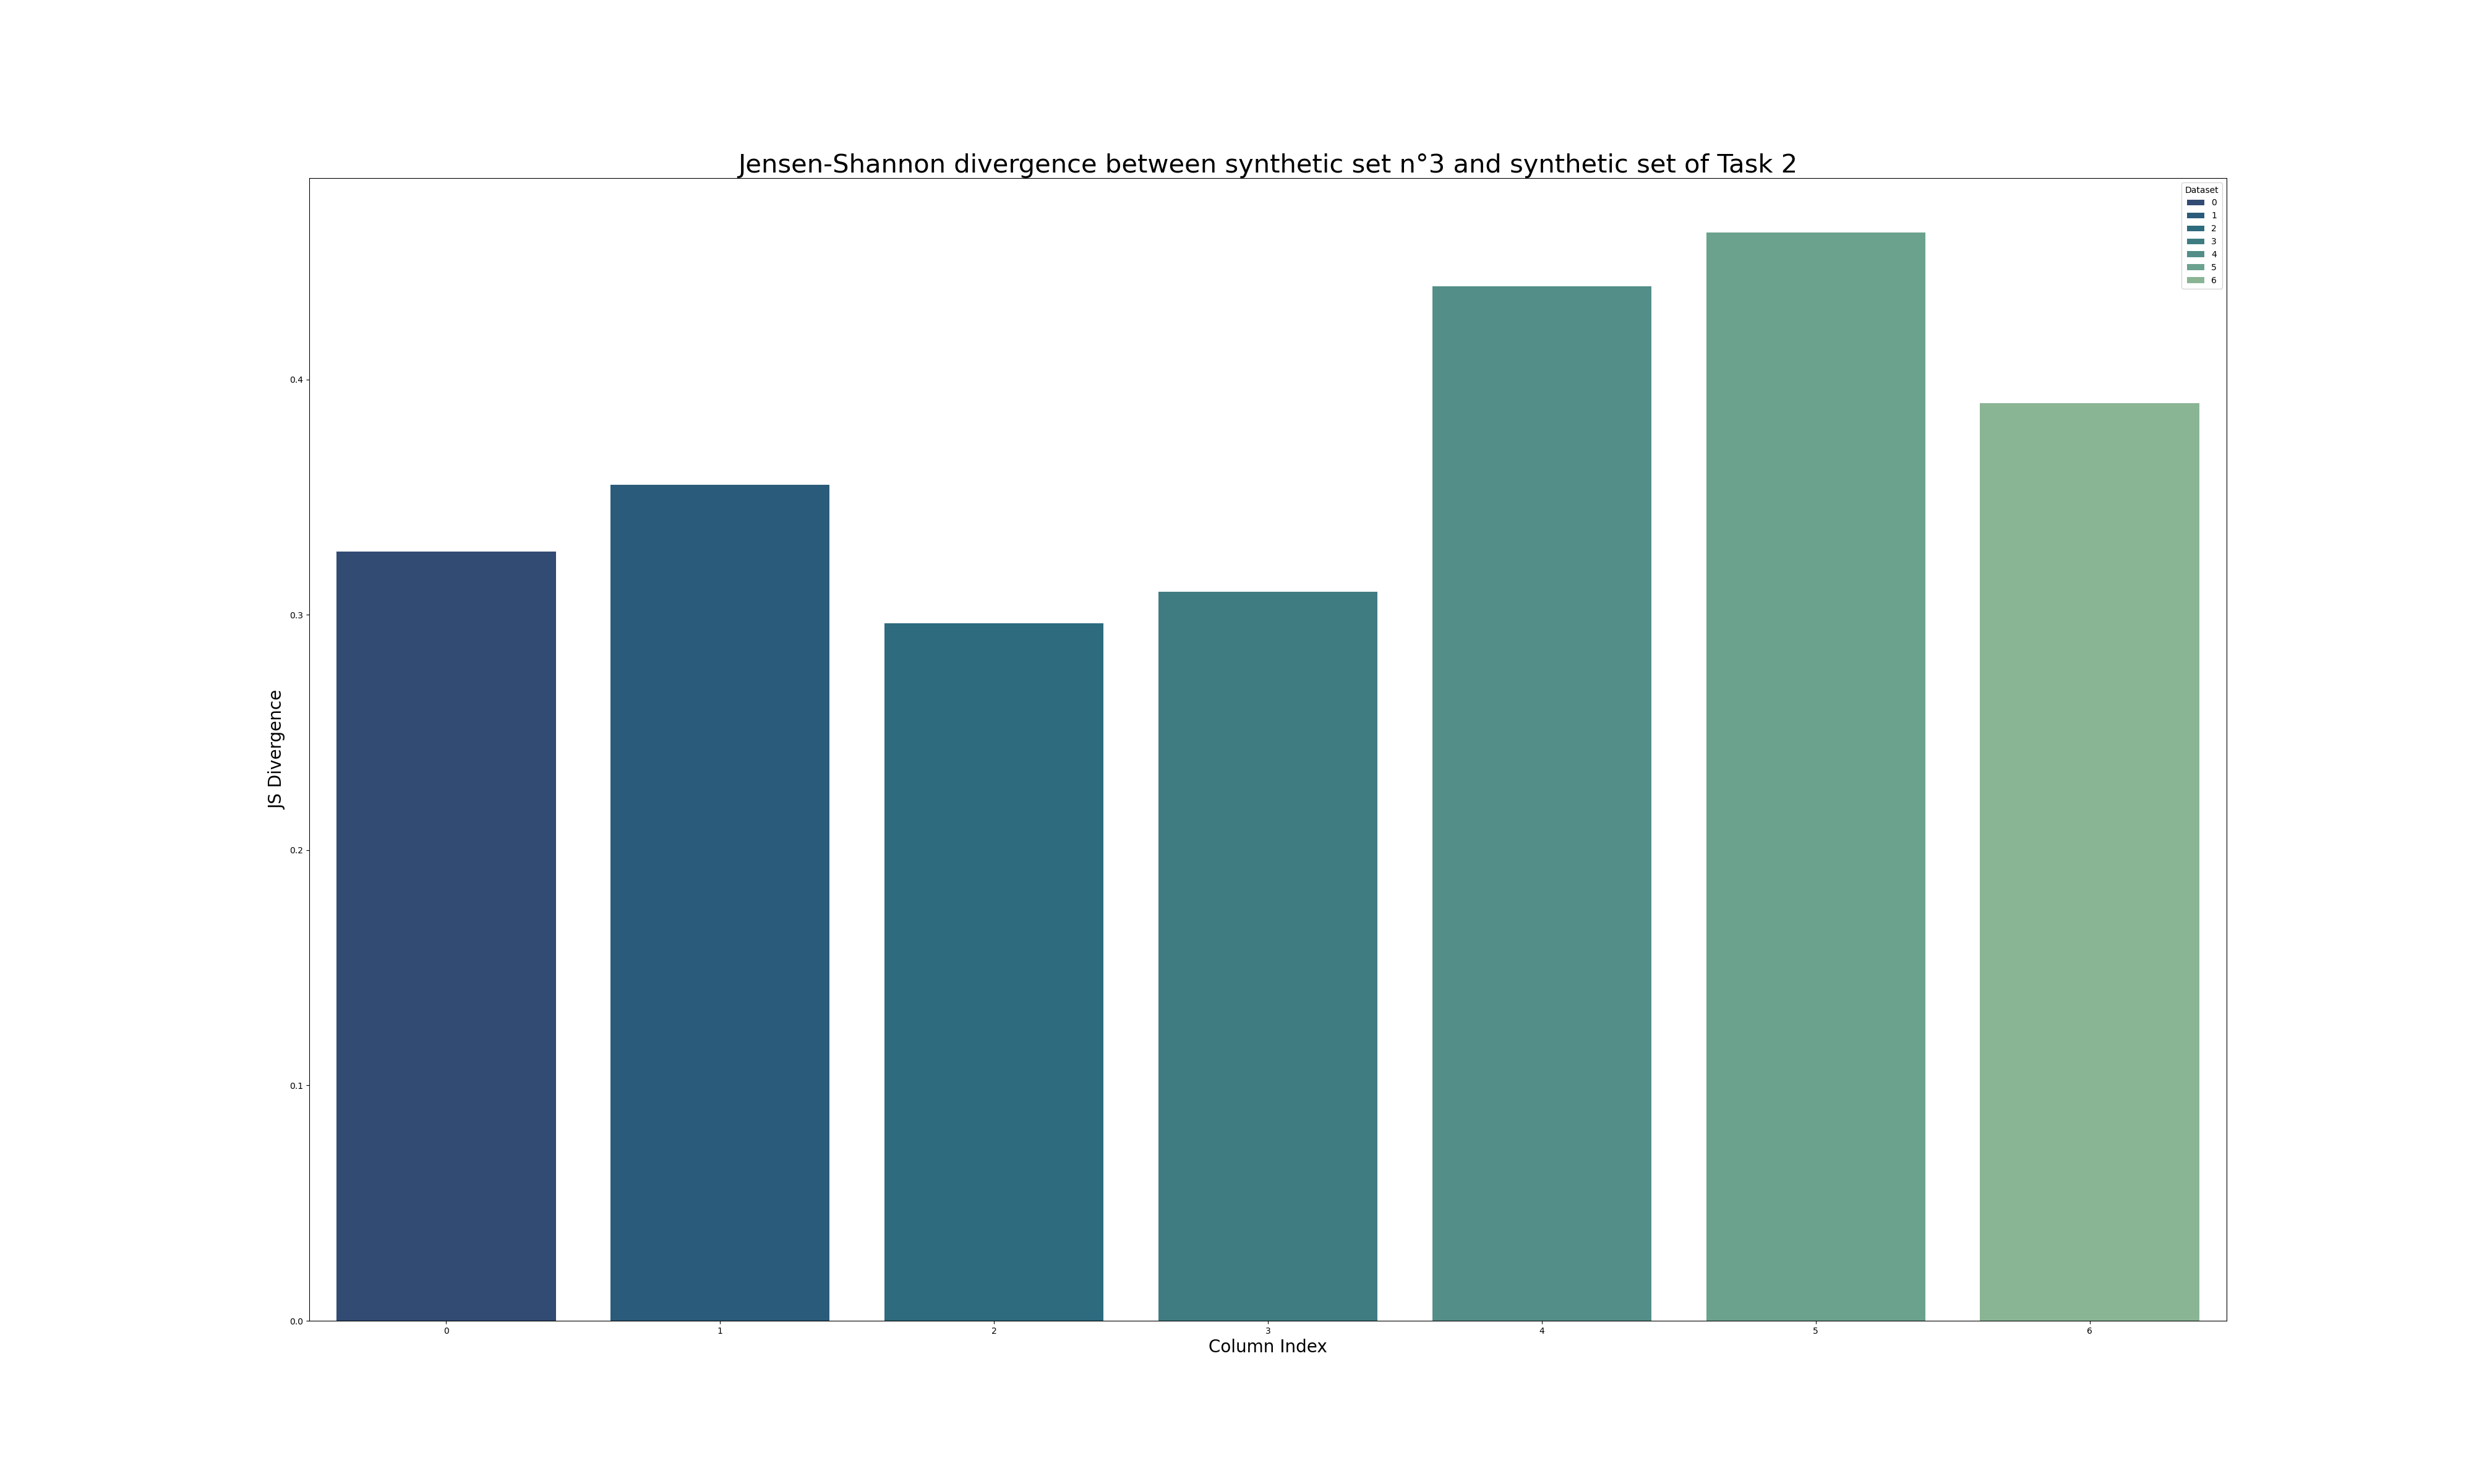
\includegraphics[width = 0.28\textwidth]{figures/Resultats/JSDivergences/3}}}\qquad
                \subfloat[]{\fbox{
                    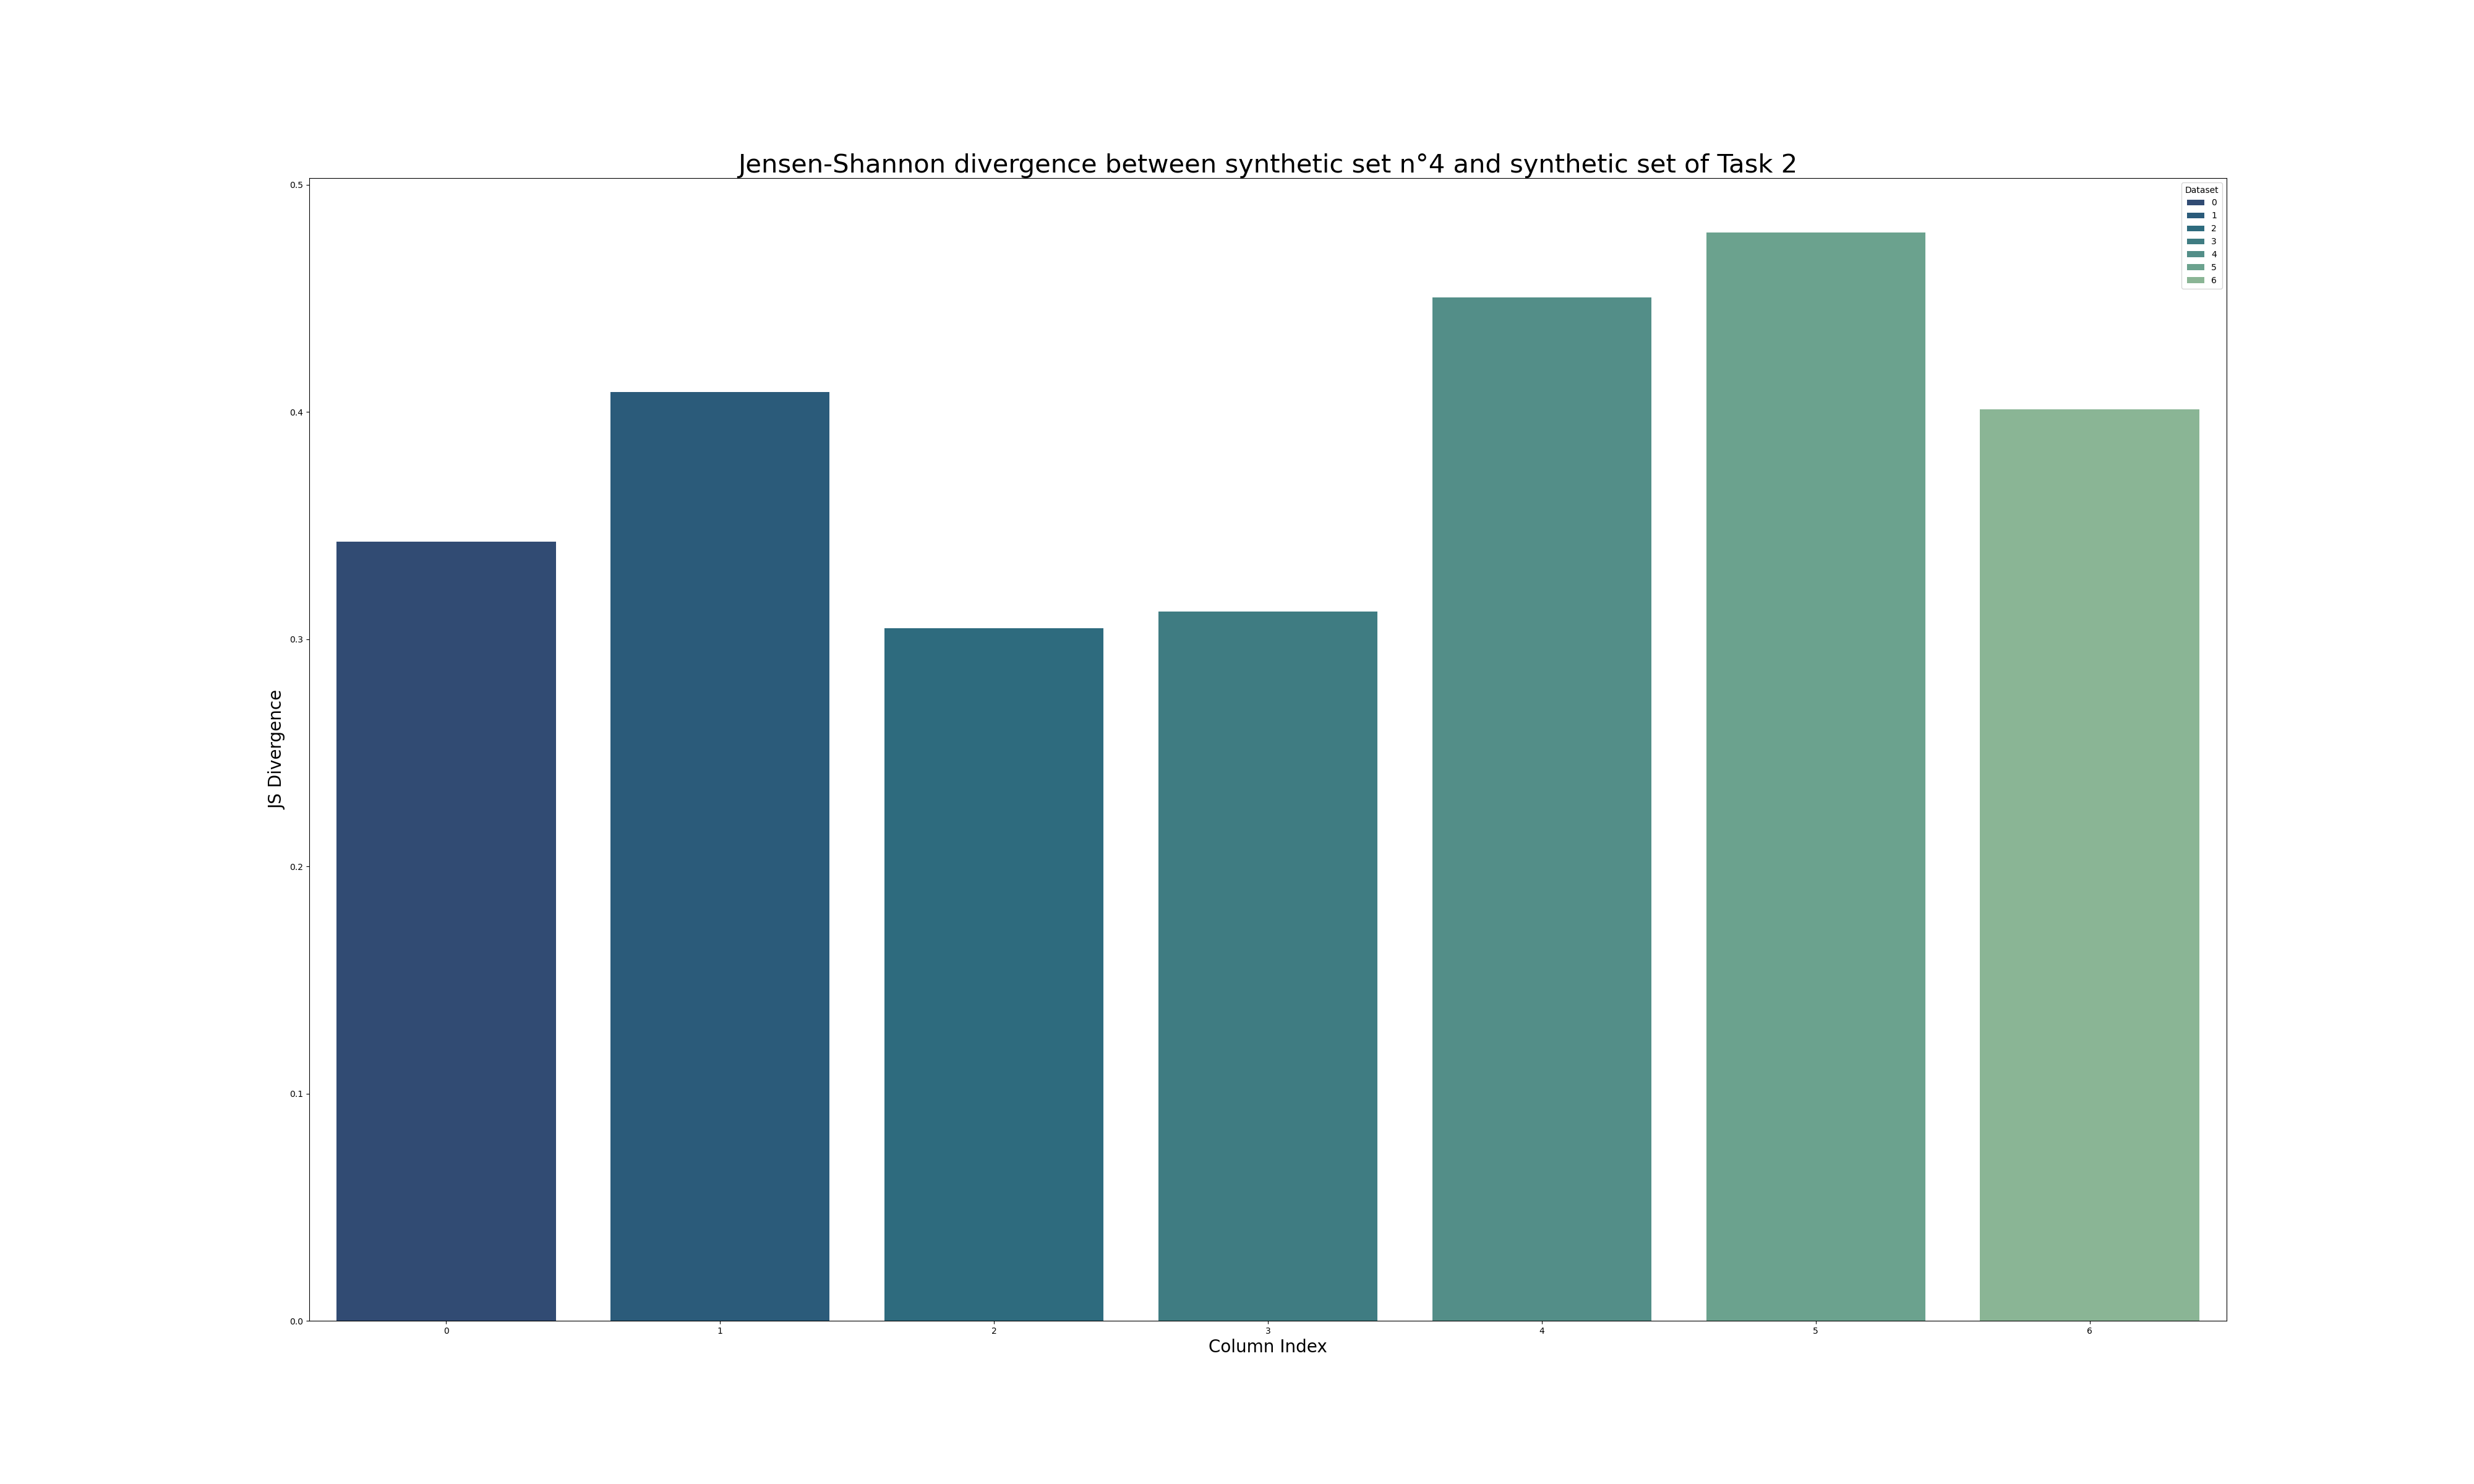
\includegraphics[width = 0.28\textwidth]{figures/Resultats/JSDivergences/4}}}\qquad
                \subfloat[]{\fbox{
                    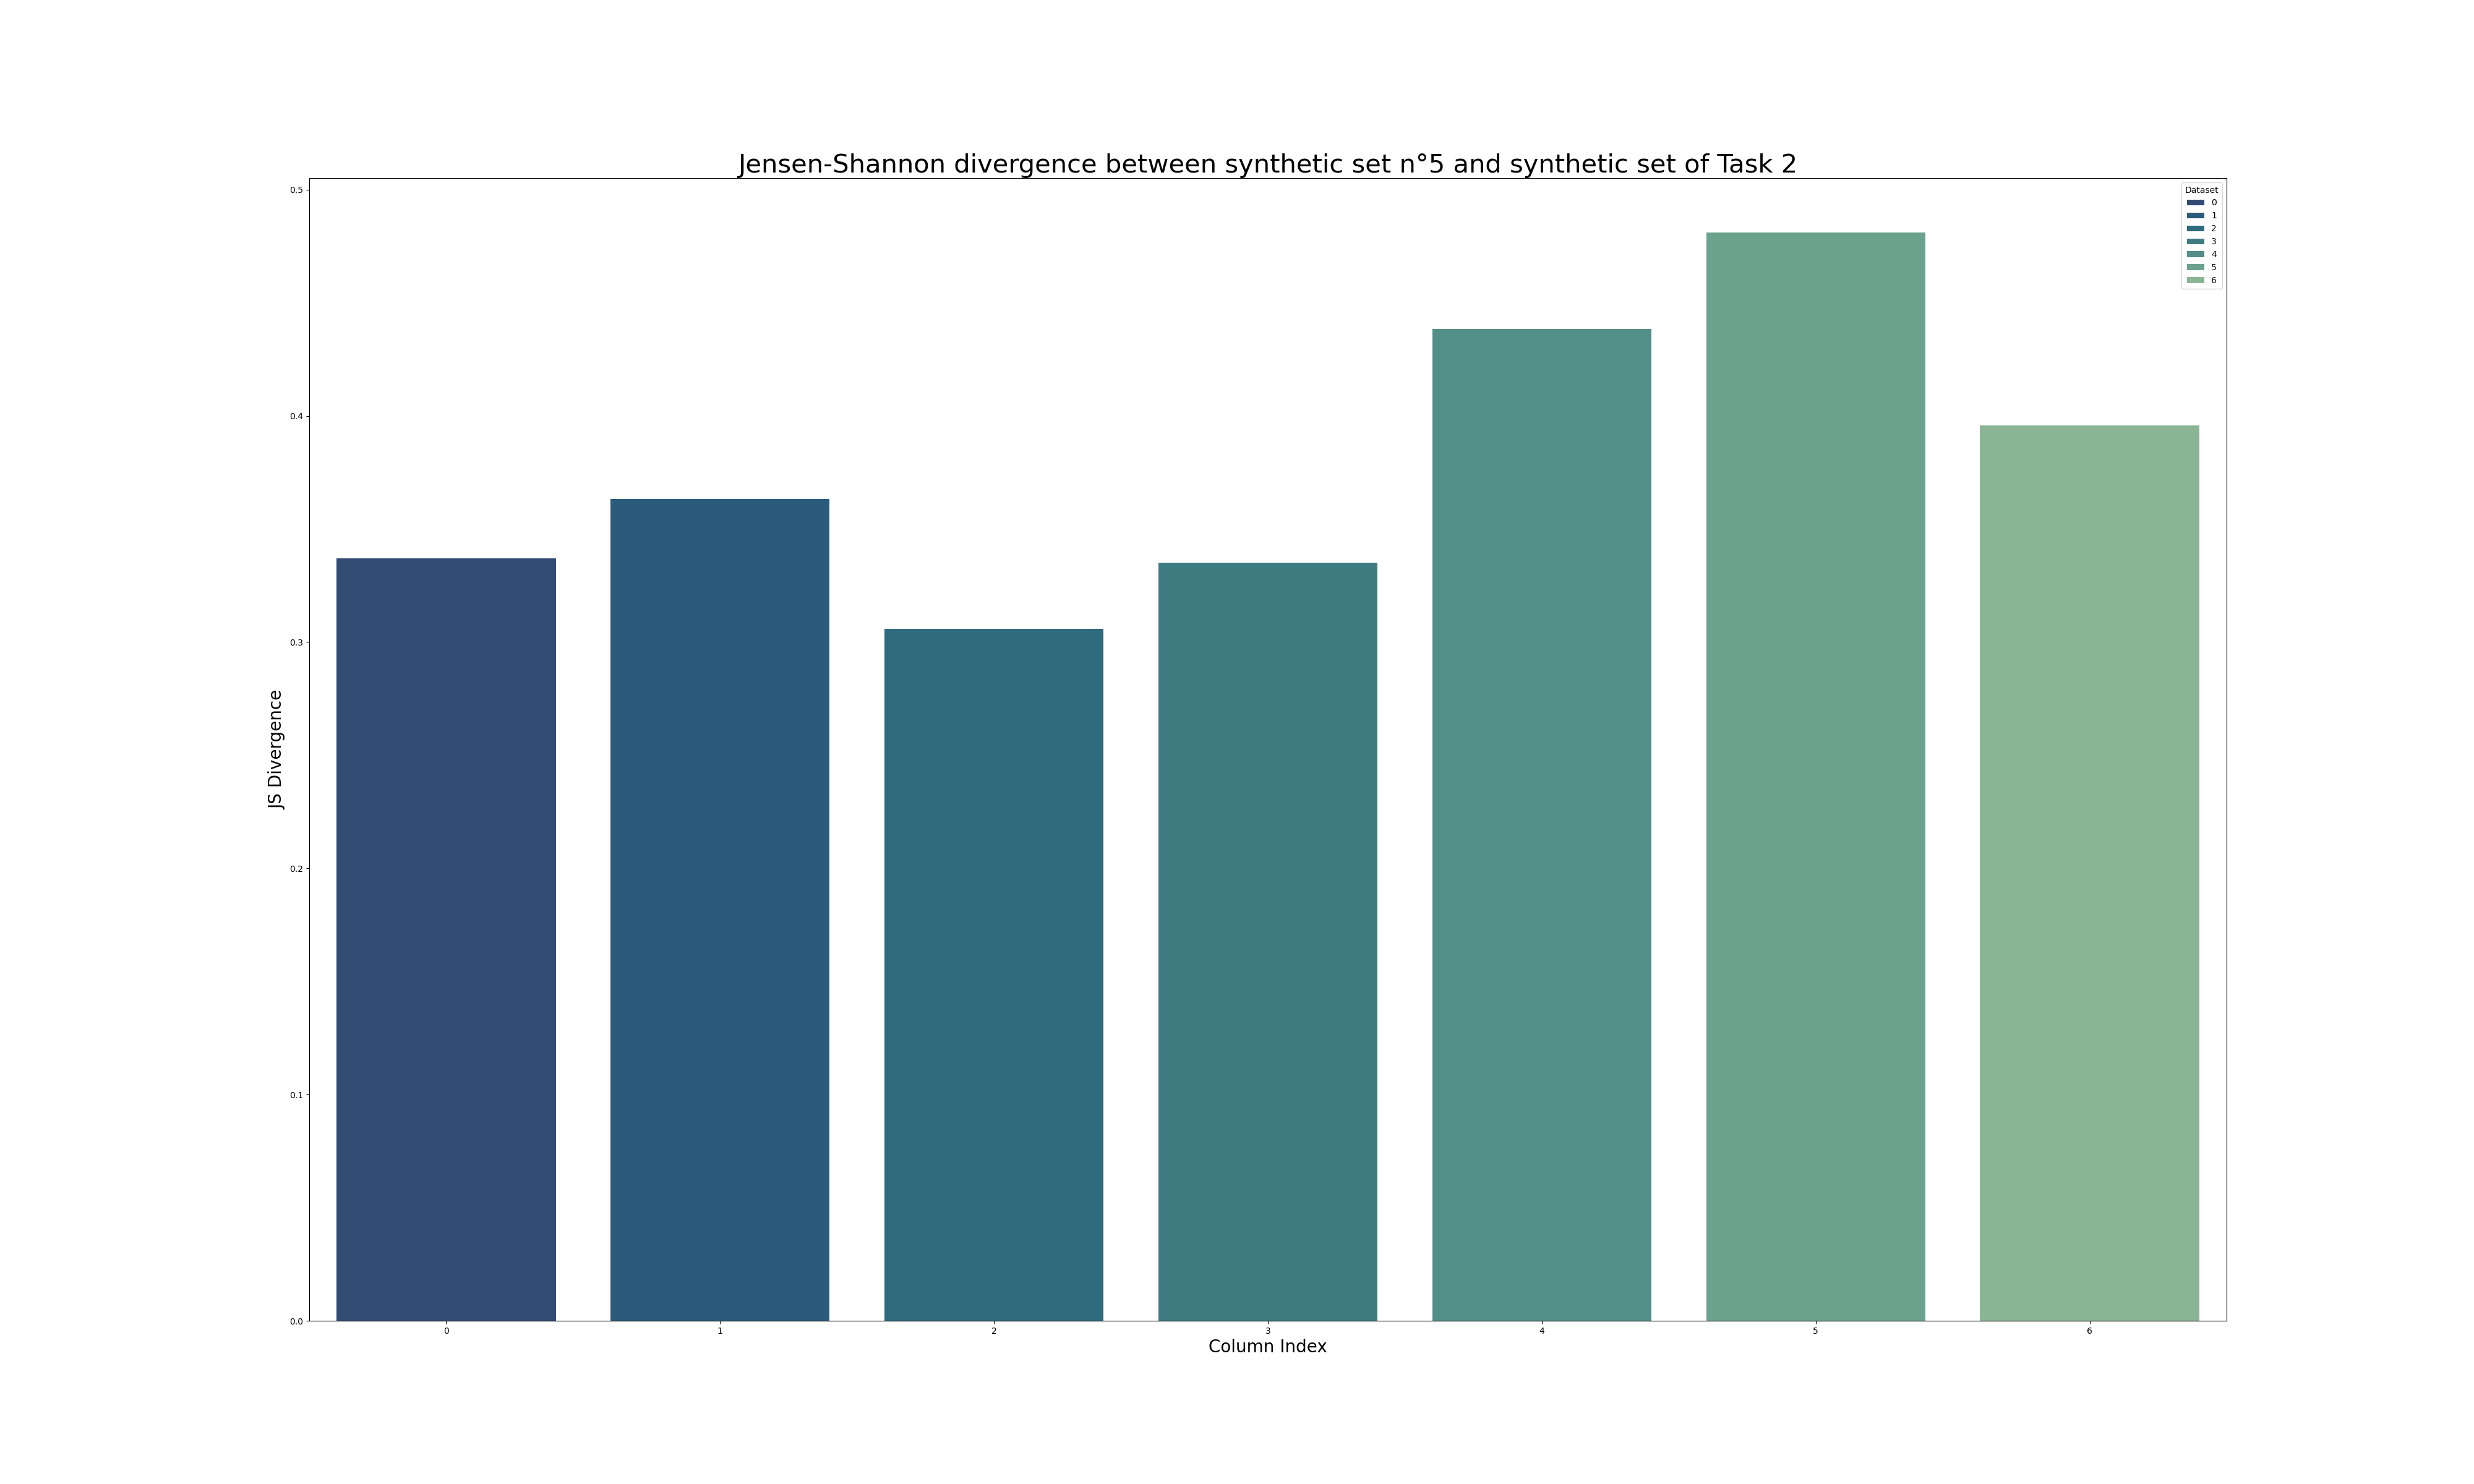
\includegraphics[width = 0.28\textwidth]{figures/Resultats/JSDivergences/5}}}\qquad
                \subfloat[]{\fbox{
                    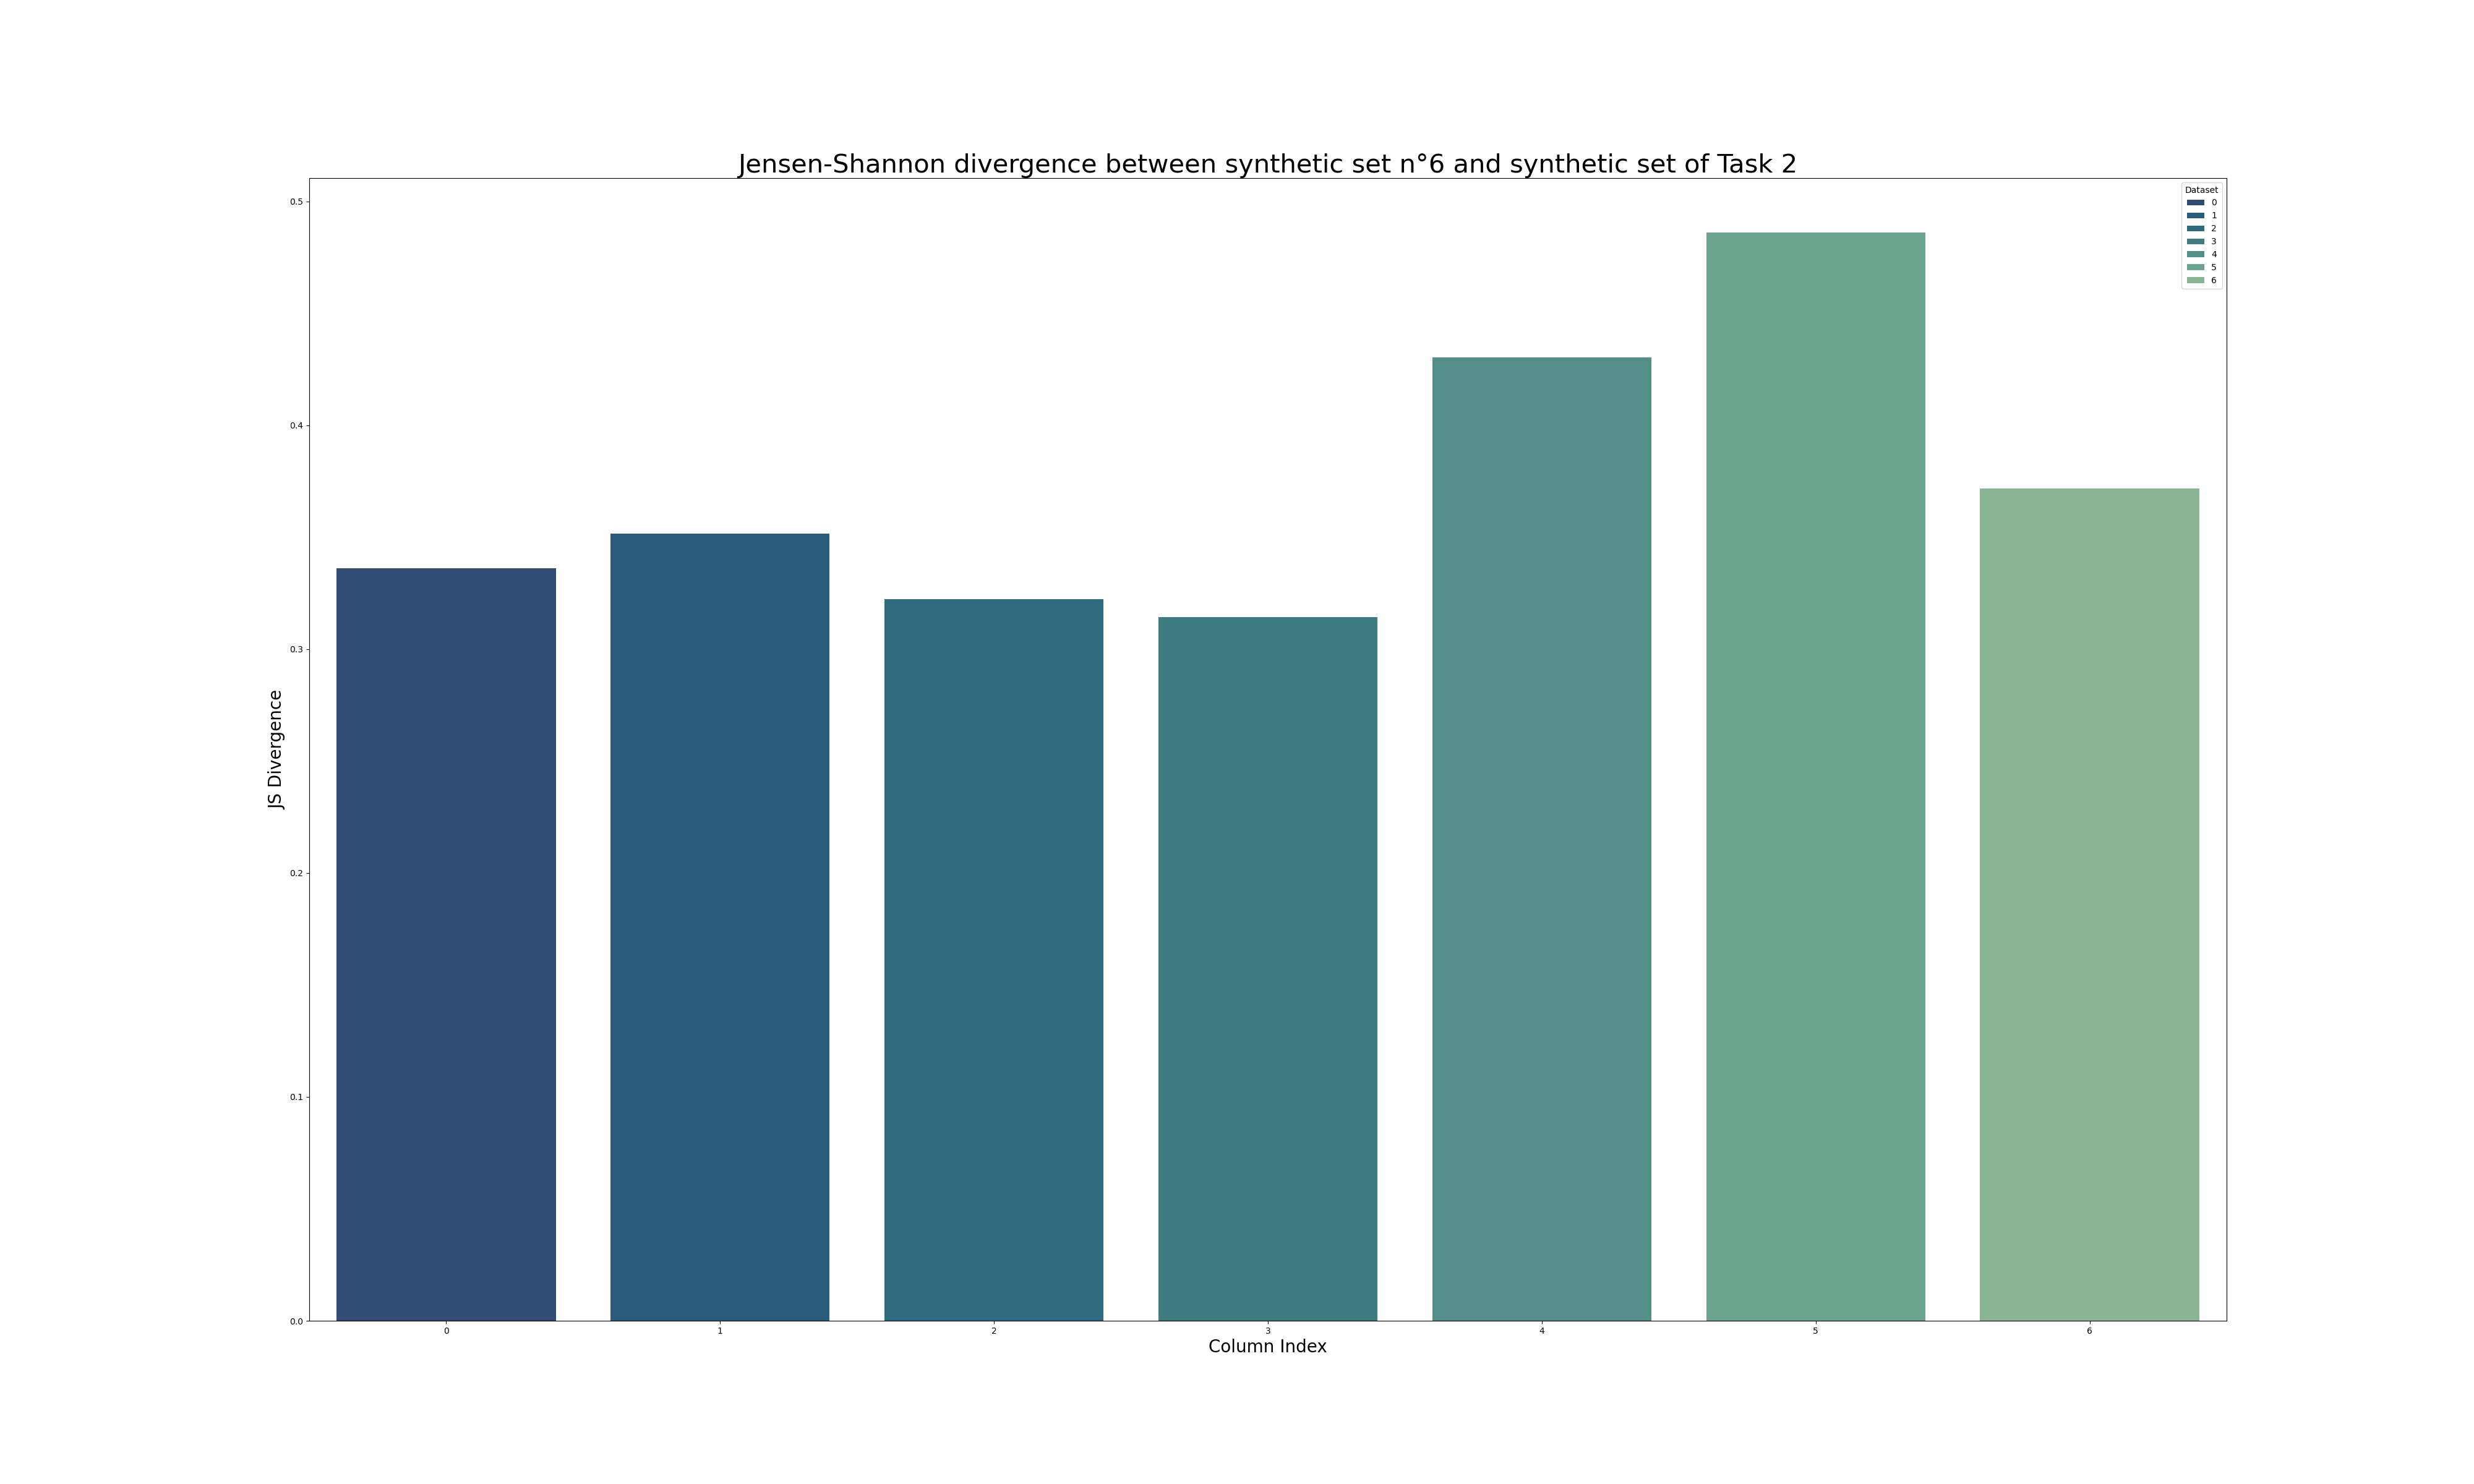
\includegraphics[width = 0.28\textwidth]{figures/Resultats/JSDivergences/6}}}\qquad
                \subfloat[]{\fbox{
                    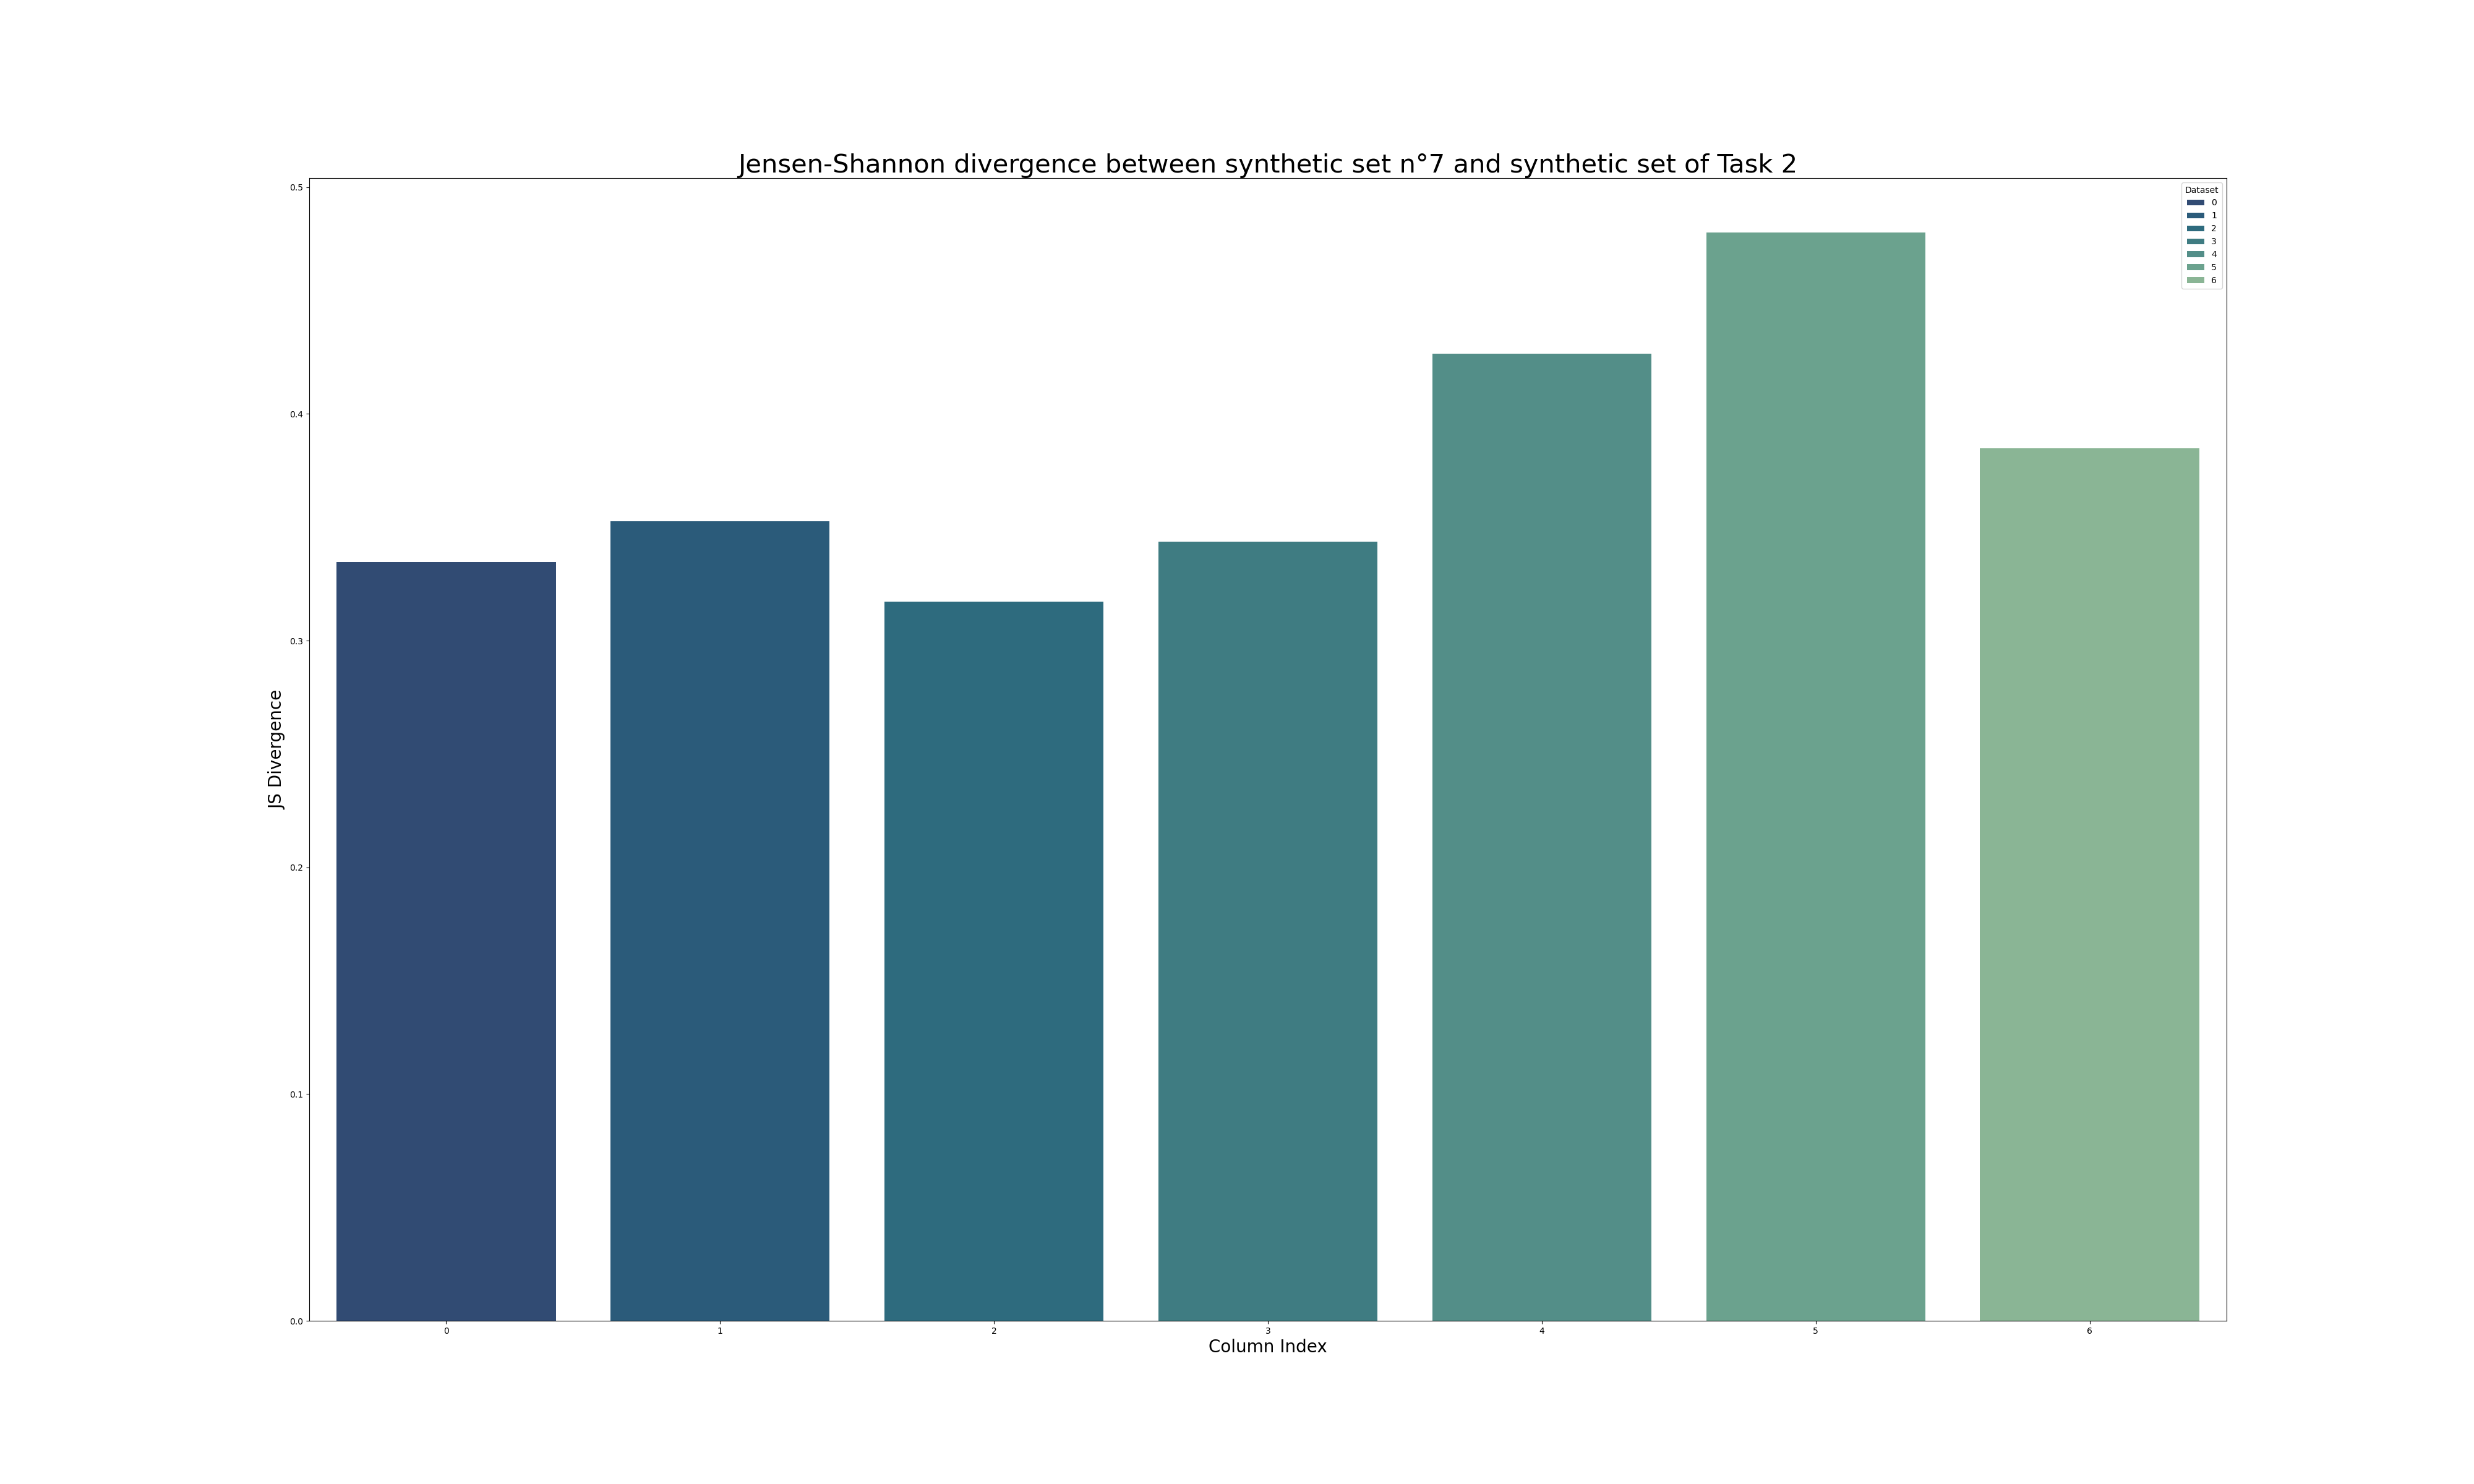
\includegraphics[width = 0.28\textwidth]{figures/Resultats/JSDivergences/7}}}\qquad
                \subfloat[]{\fbox{
                    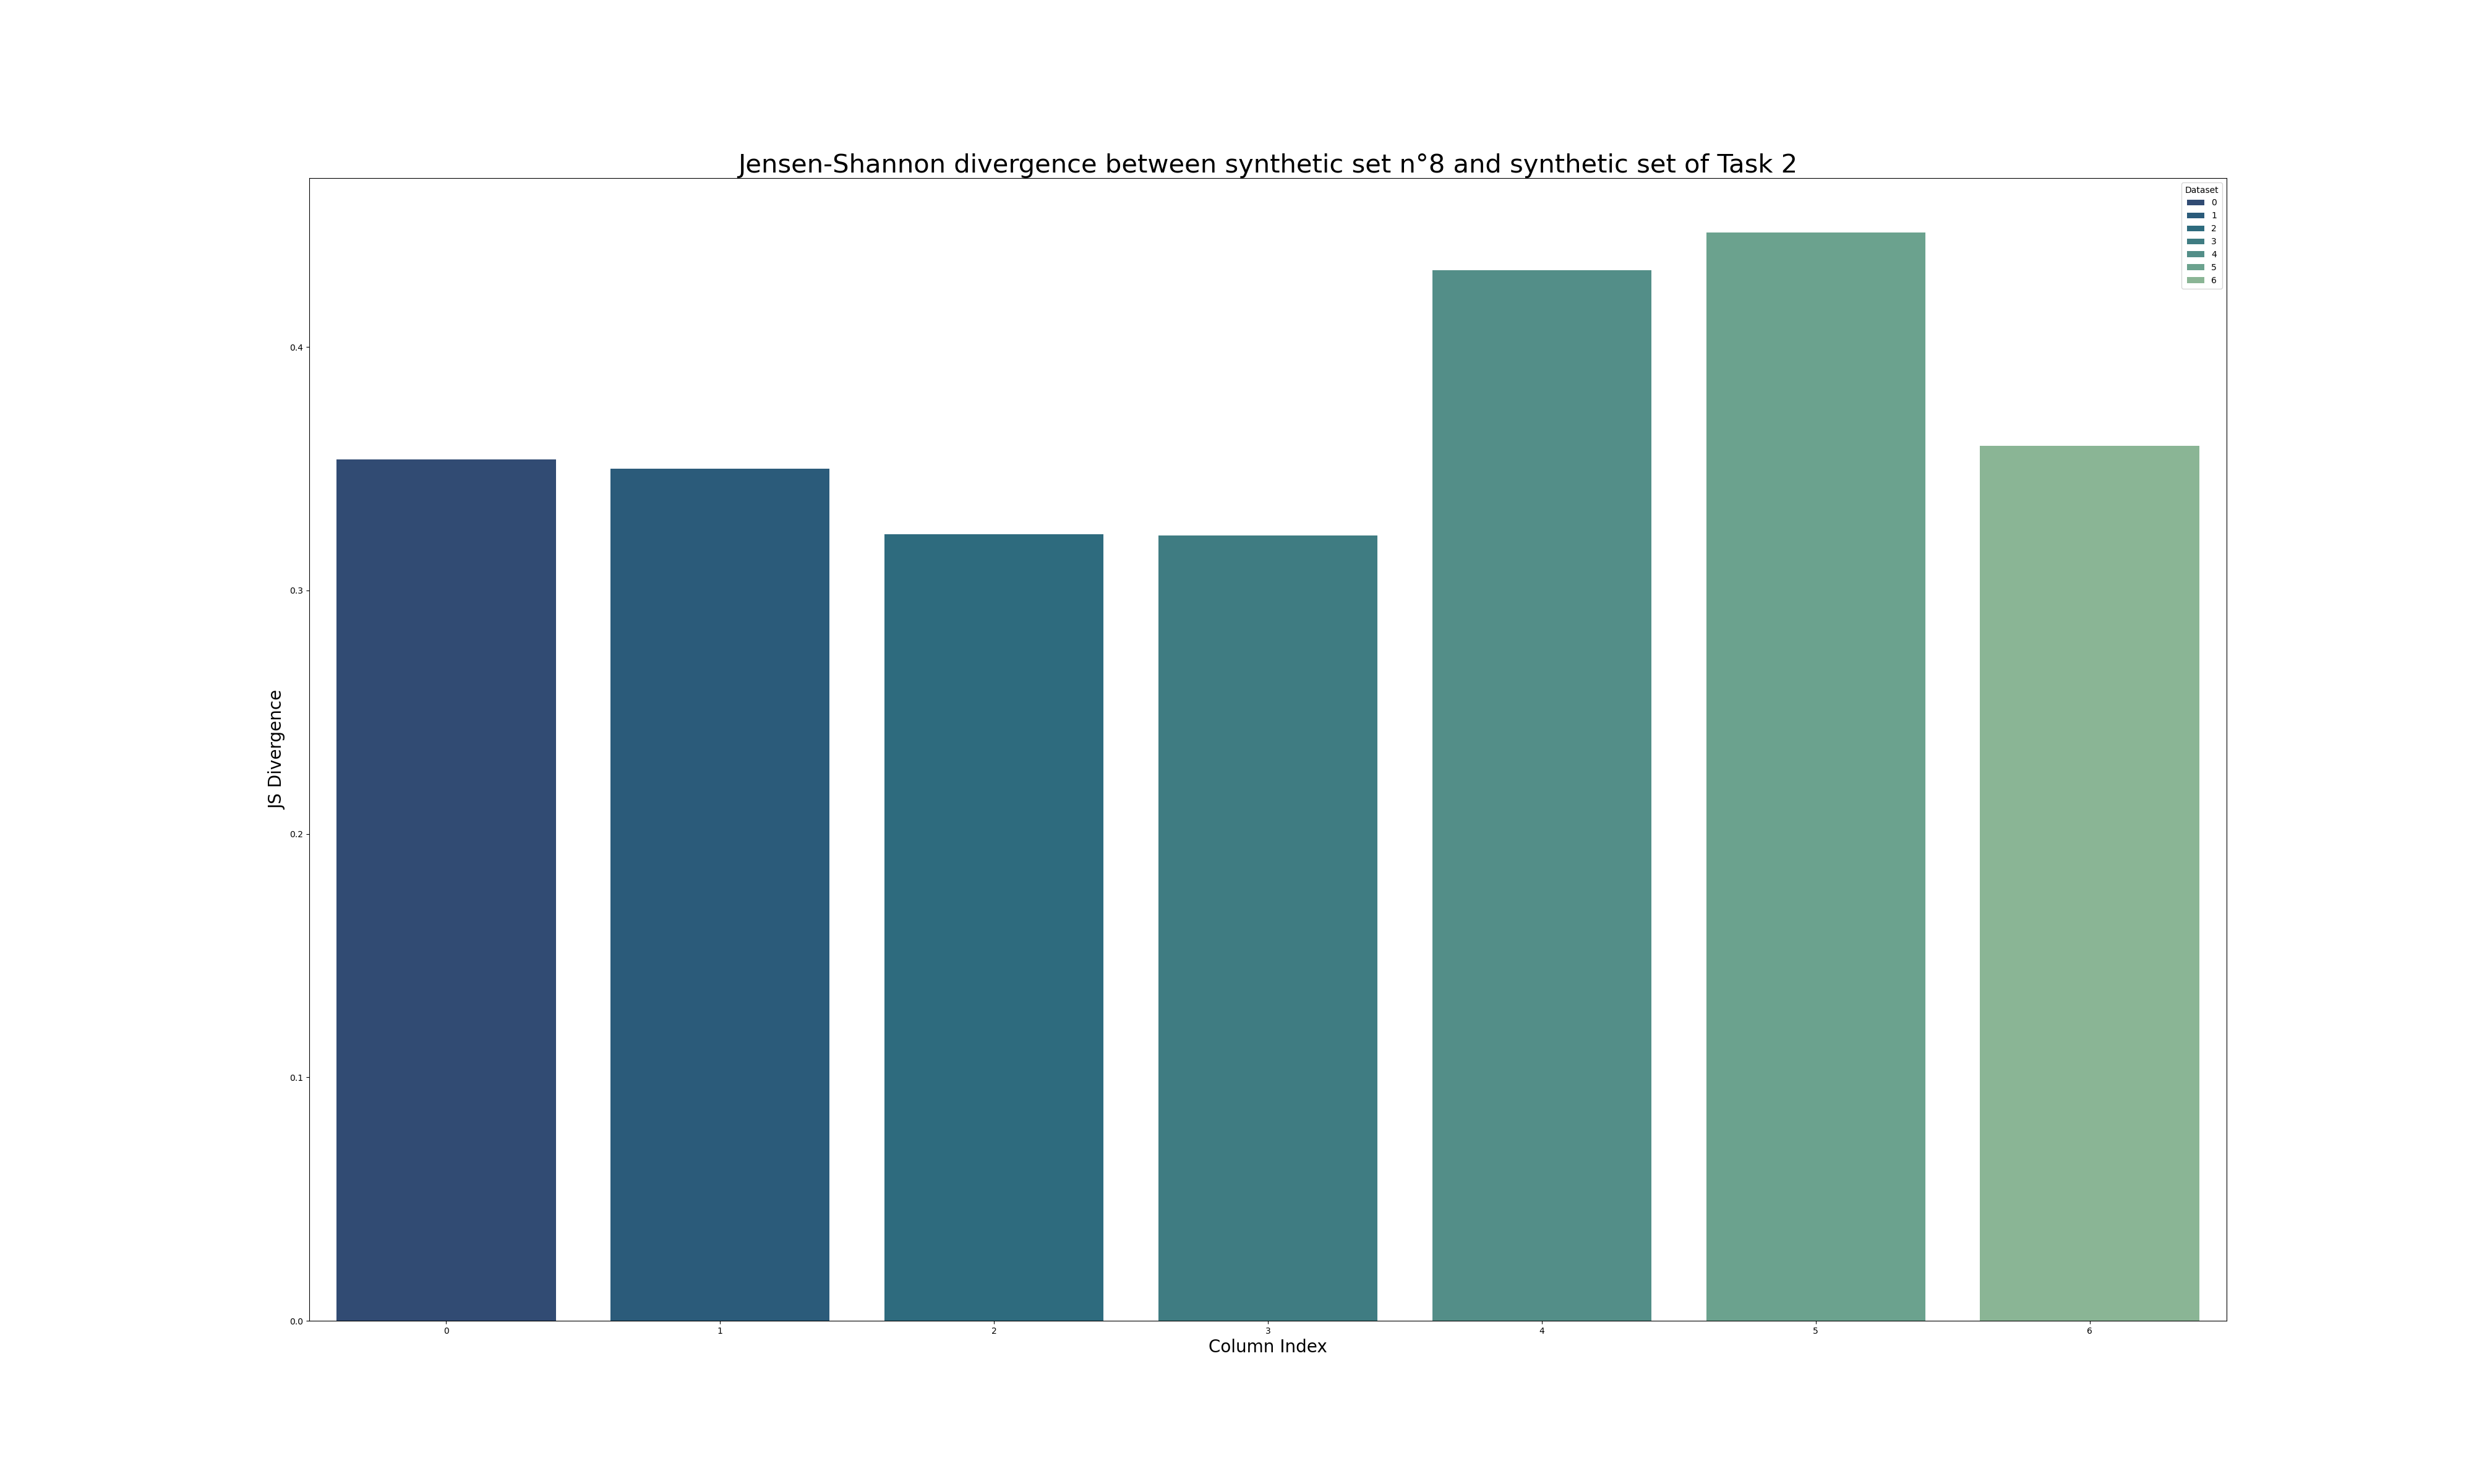
\includegraphics[width = 0.28\textwidth]{figures/Resultats/JSDivergences/8}}}\qquad
                \subfloat[]{\fbox{
                    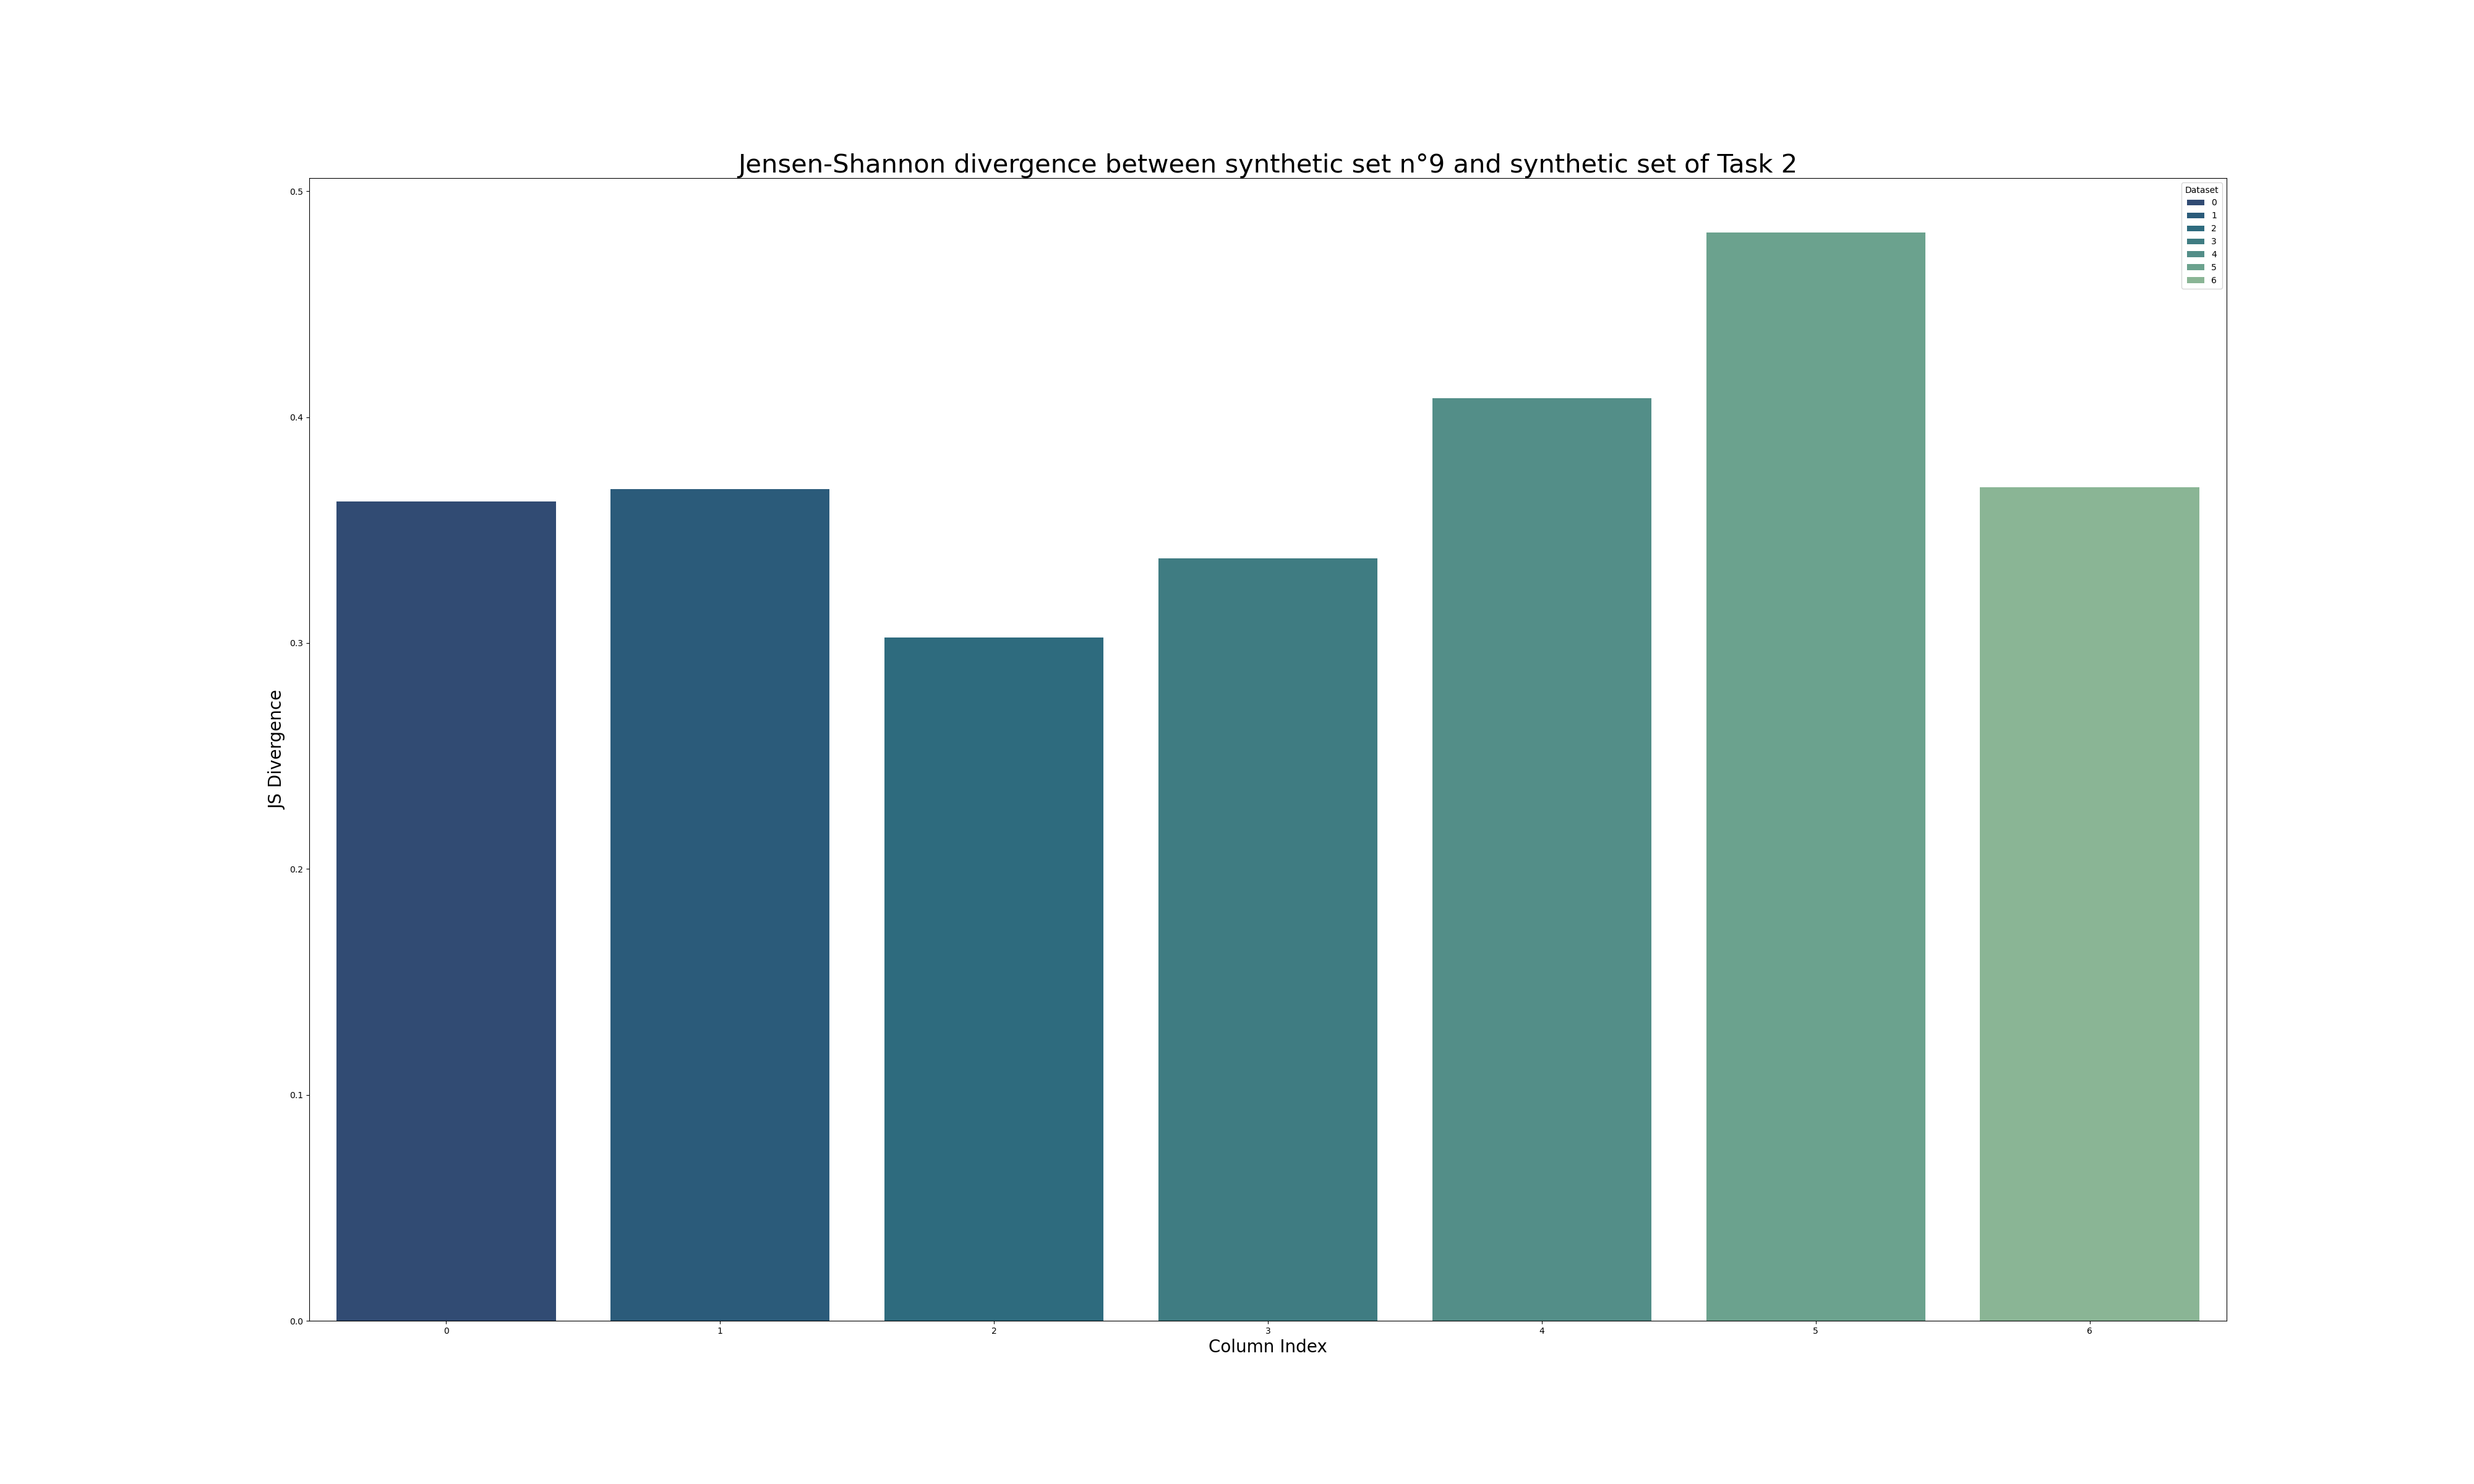
\includegraphics[width = 0.28\textwidth]{figures/Resultats/JSDivergences/9}}}\qquad
                \subfloat[]{\fbox{
                    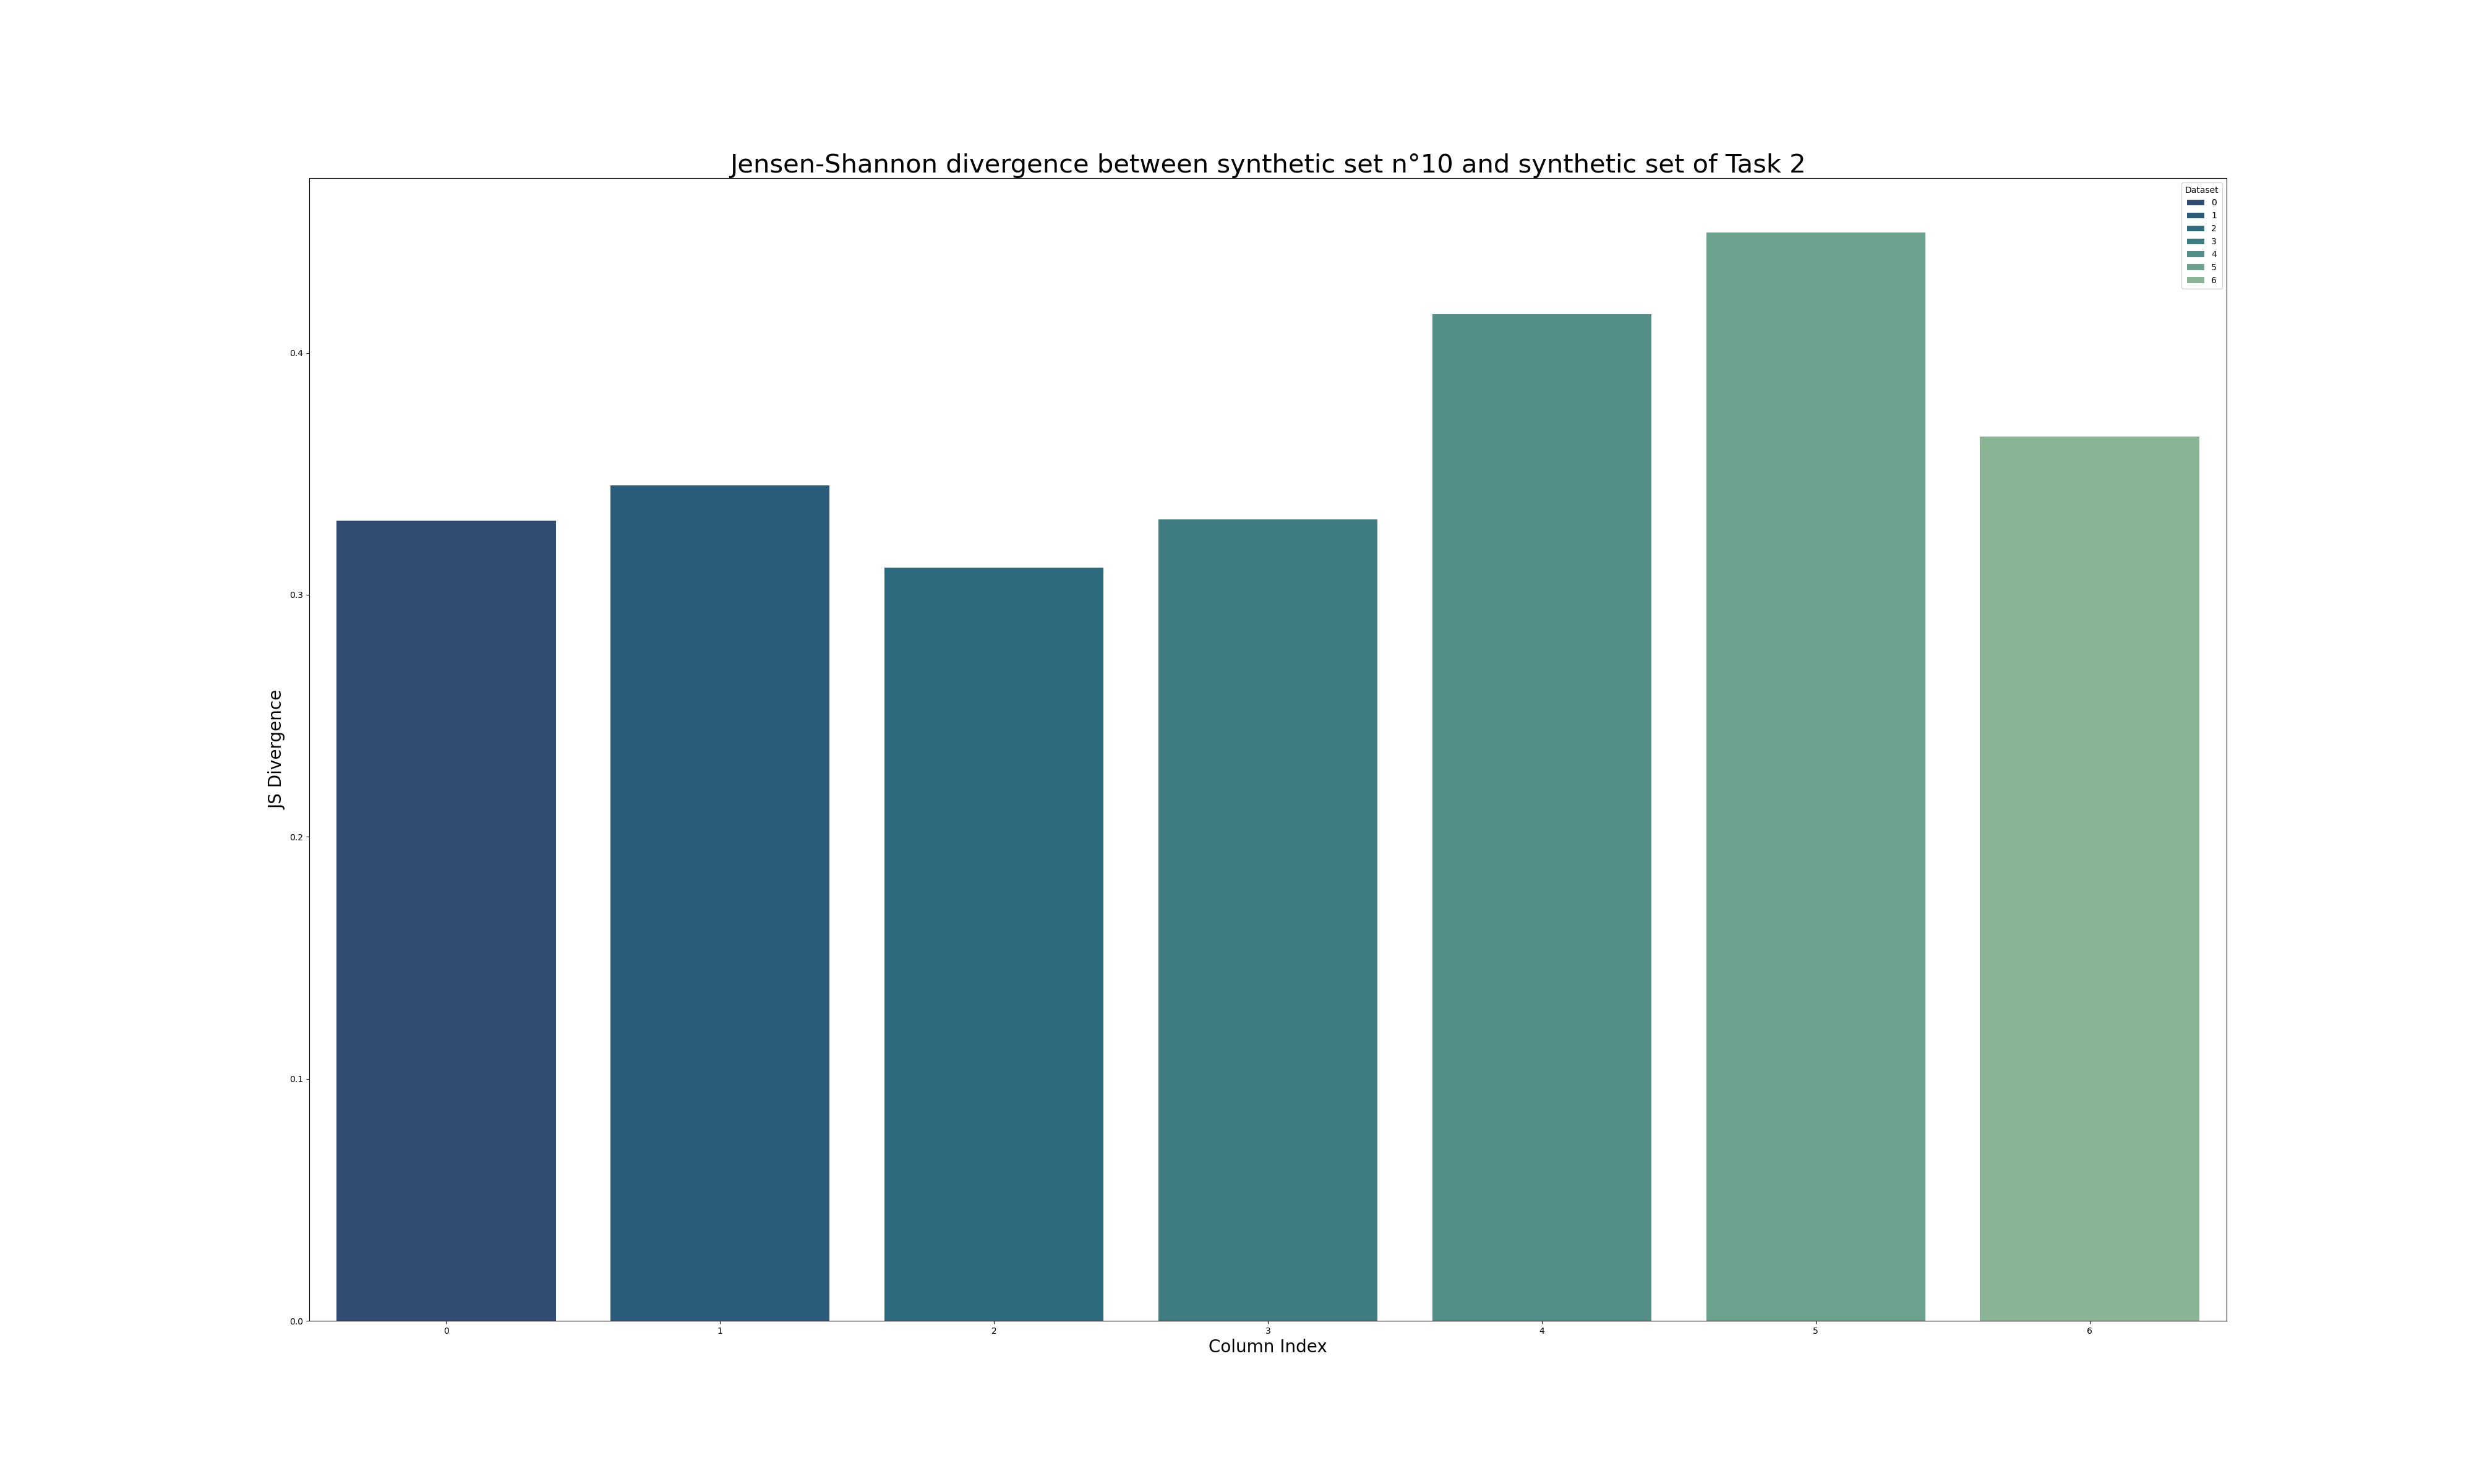
\includegraphics[width = 0.28\textwidth]{figures/Resultats/JSDivergences/10}}}\qquad
                \subfloat[]{\fbox{
                    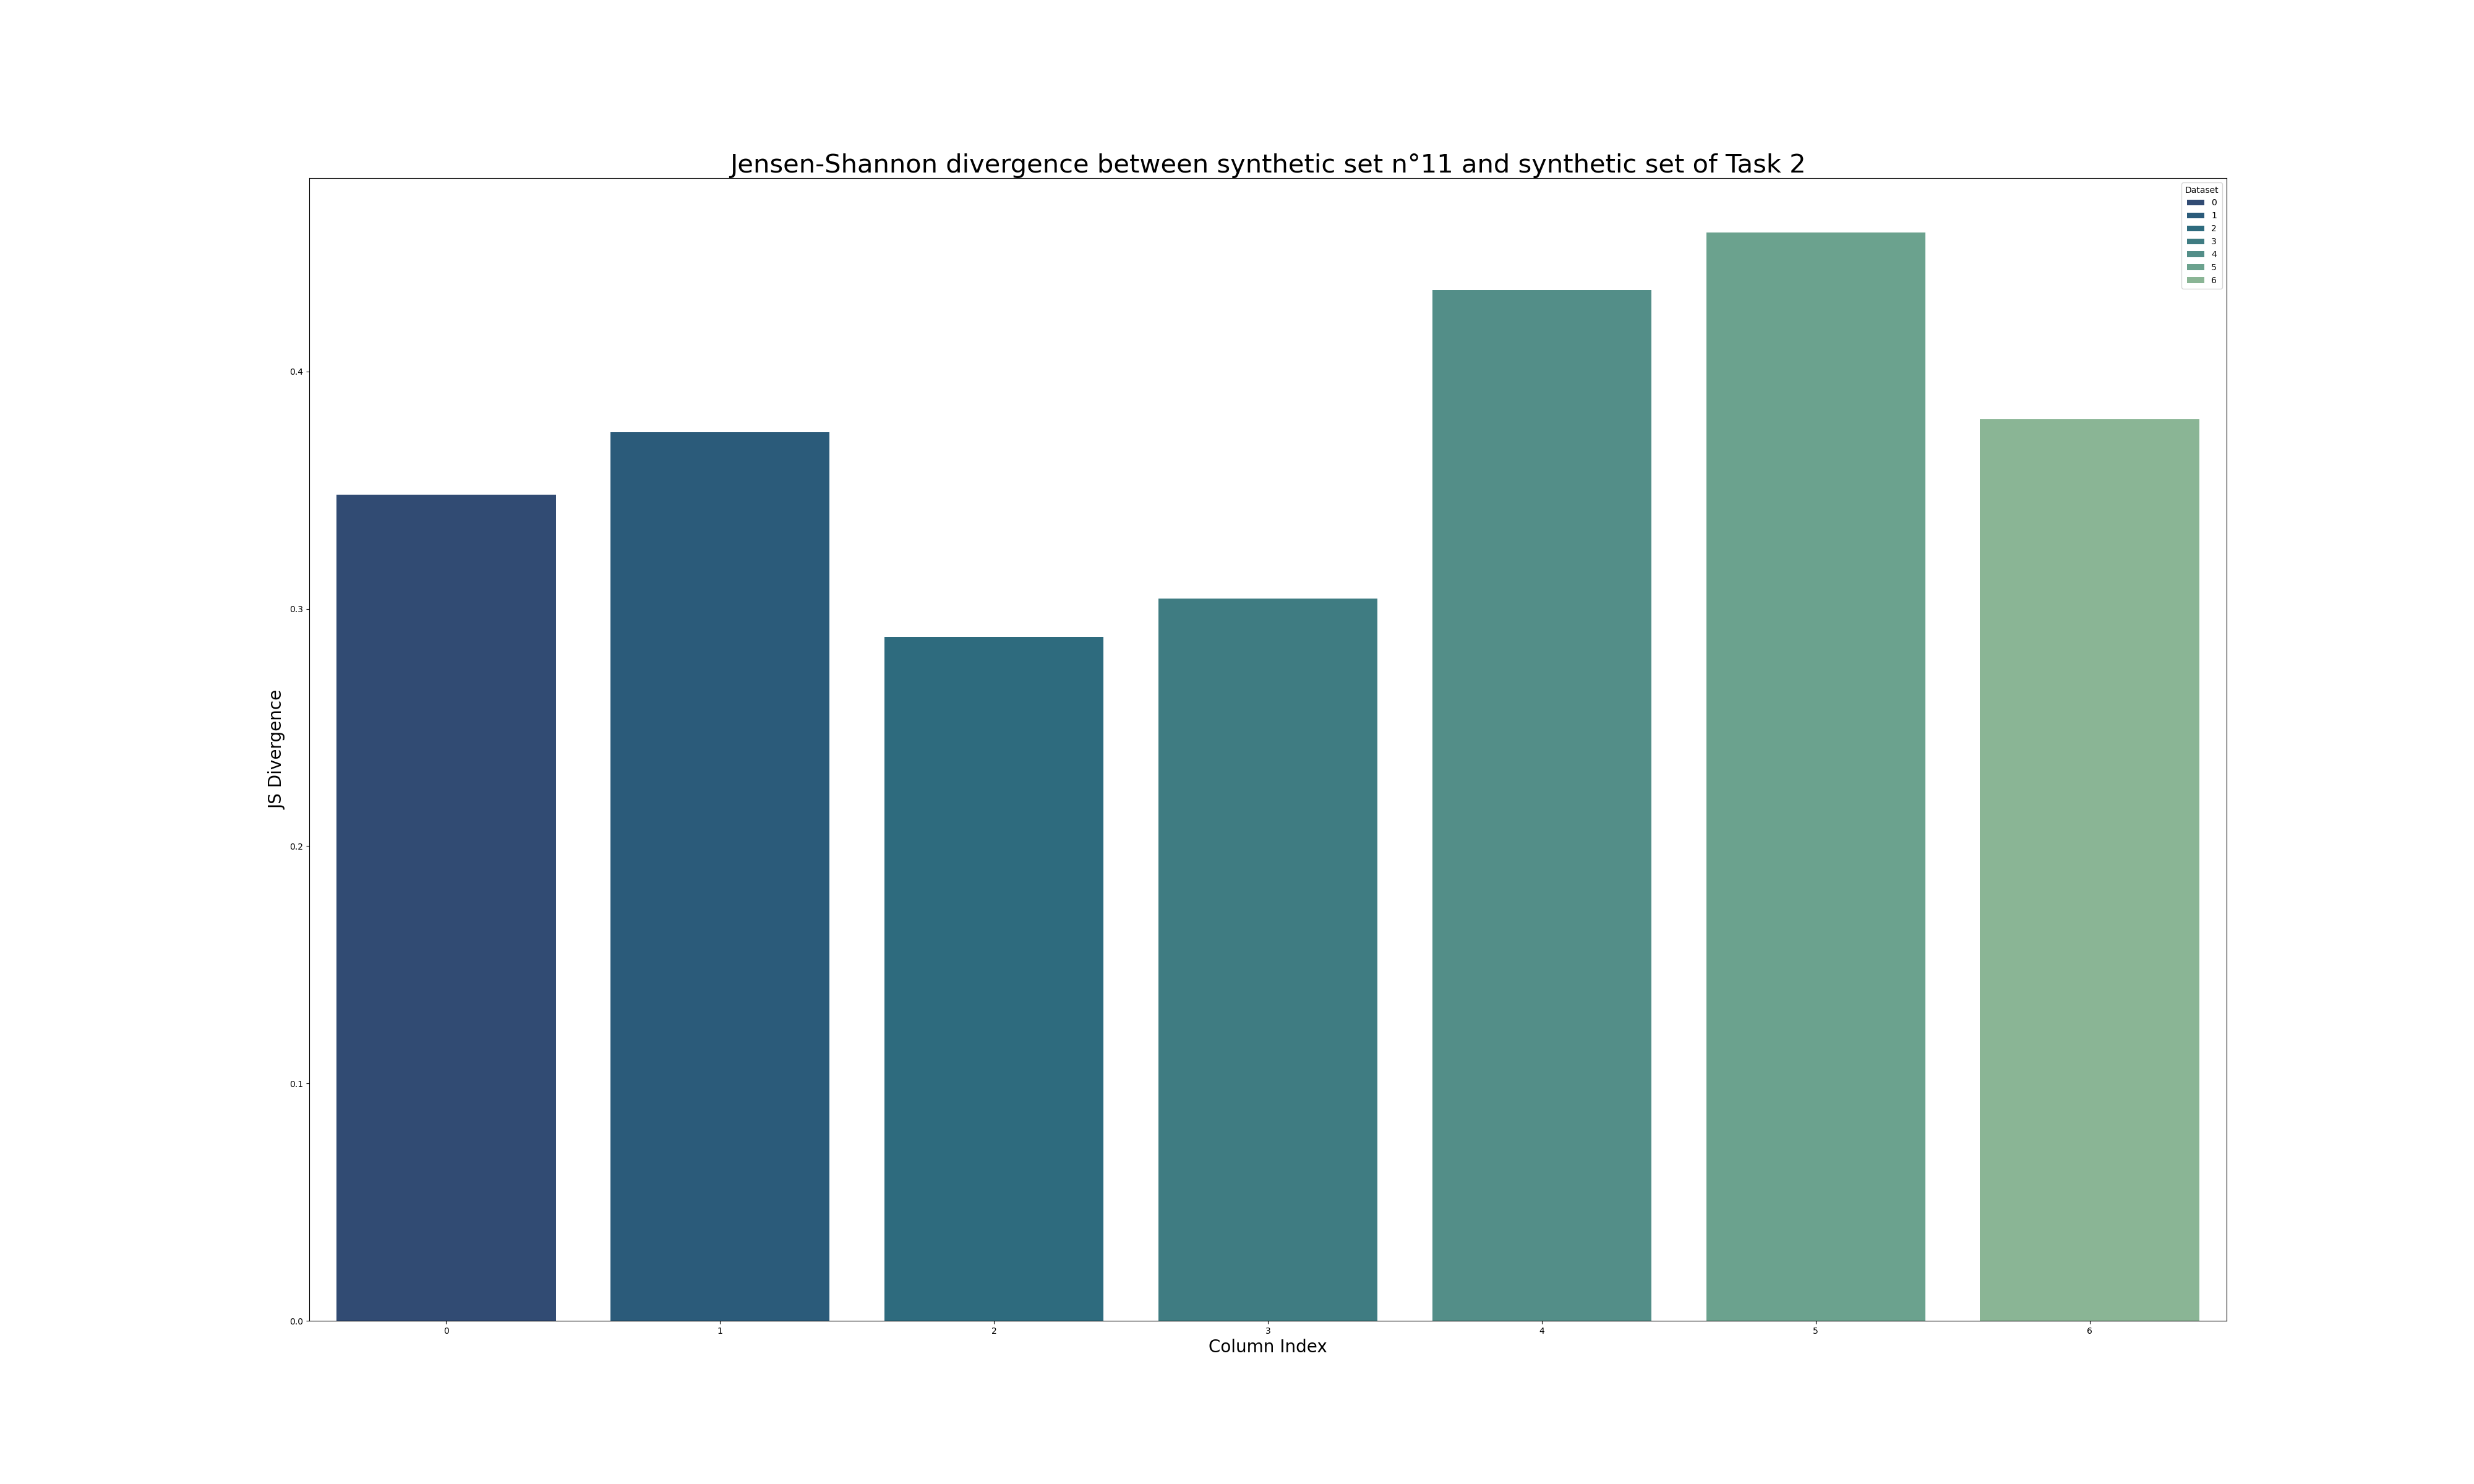
\includegraphics[width = 0.28\textwidth]{figures/Resultats/JSDivergences/11}}}\qquad
                \subfloat[]{\fbox{
                    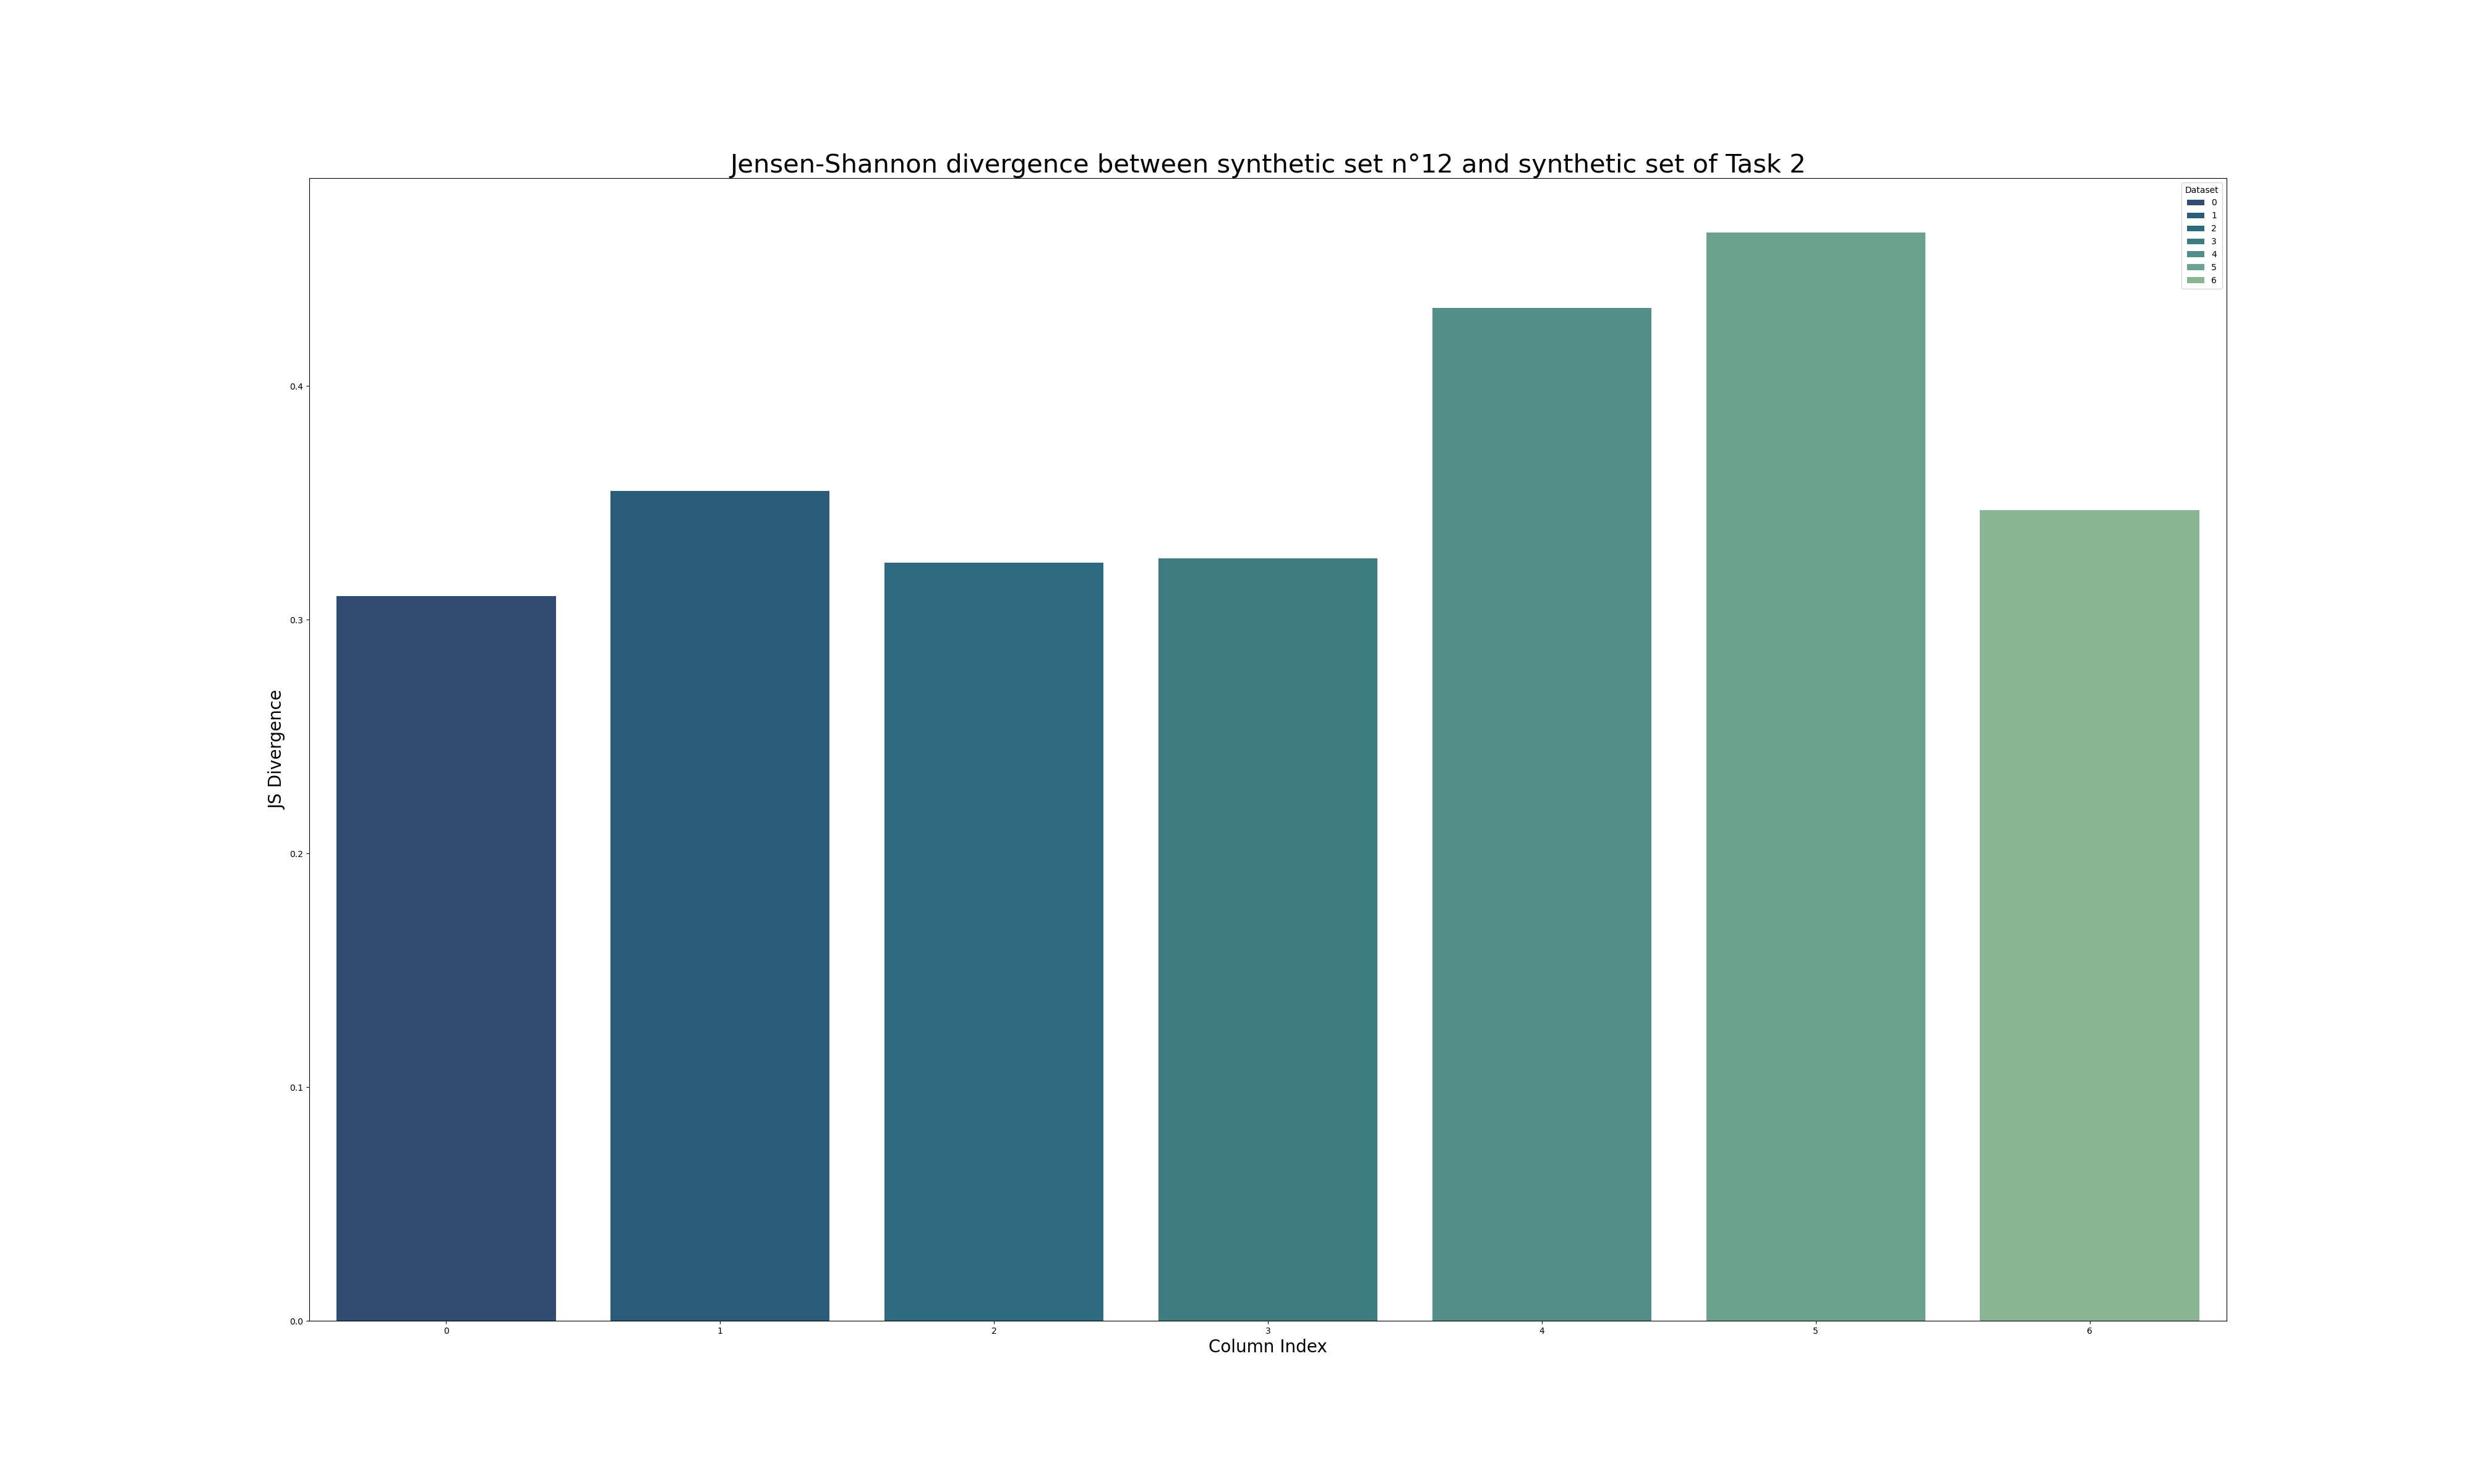
\includegraphics[width = 0.28\textwidth]{figures/Resultats/JSDivergences/12}}}\qquad
                \subfloat[]{\fbox{
                    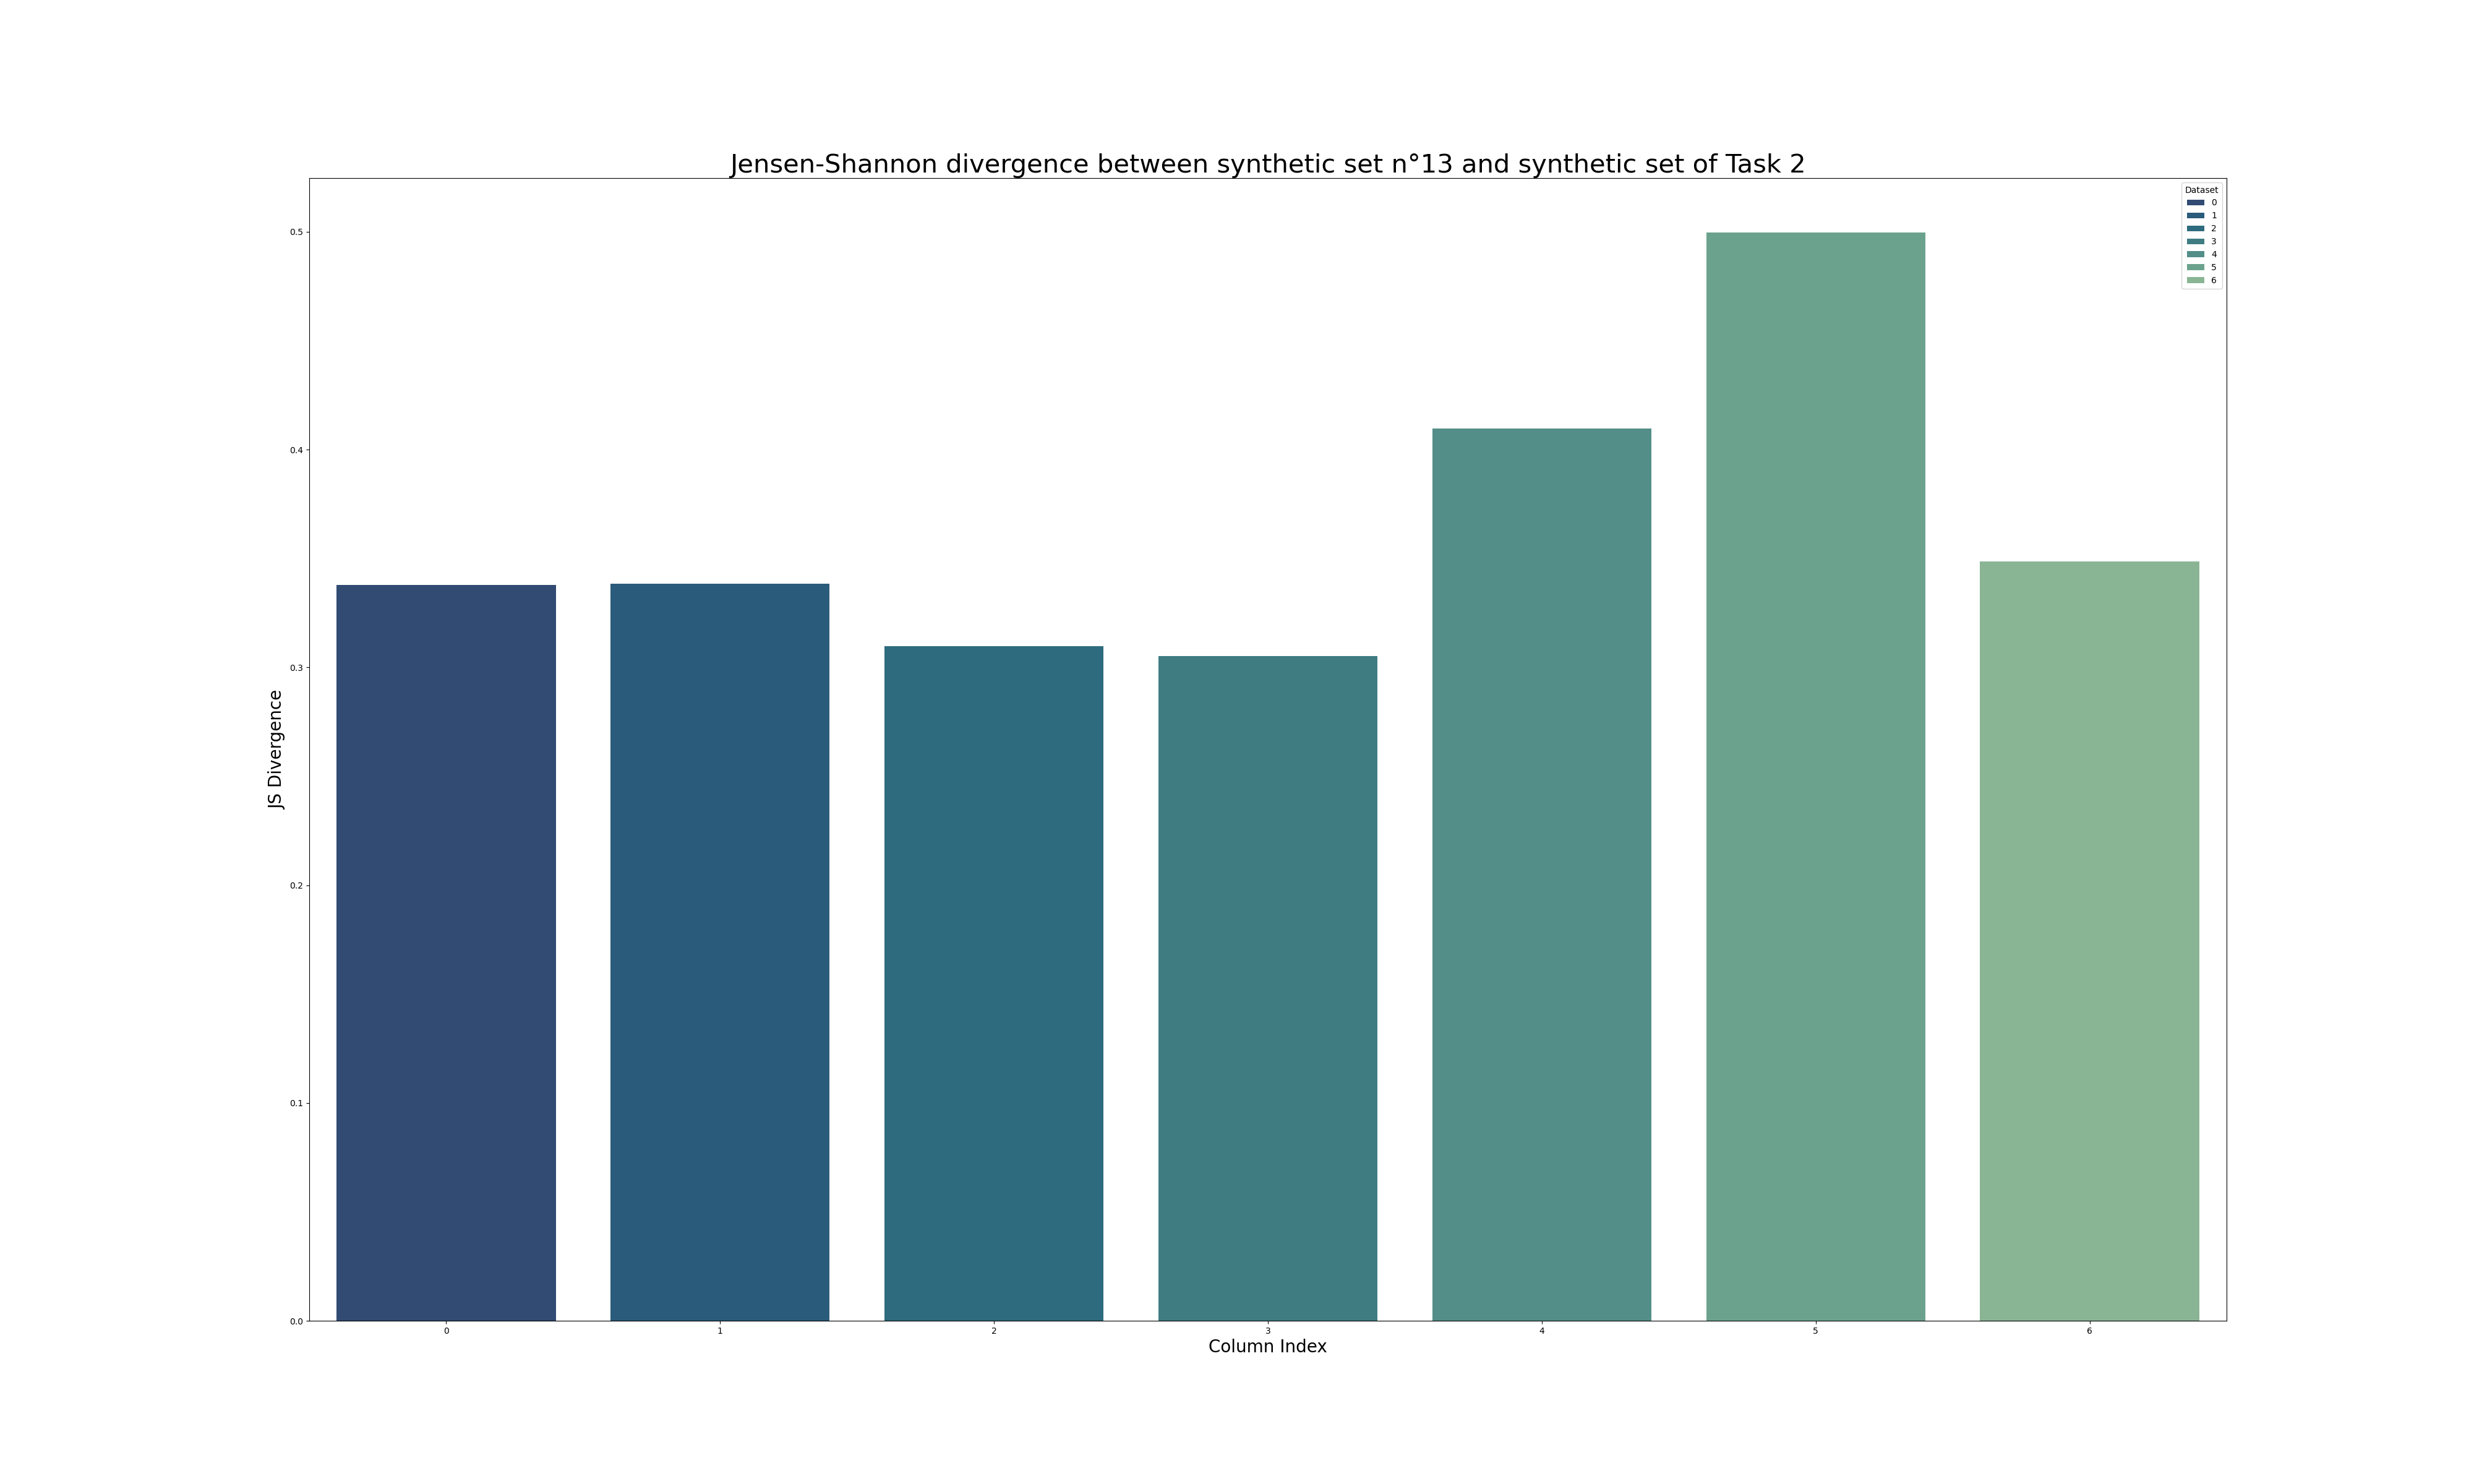
\includegraphics[width = 0.28\textwidth]{figures/Resultats/JSDivergences/13}}}\qquad
                \subfloat[]{\fbox{
                    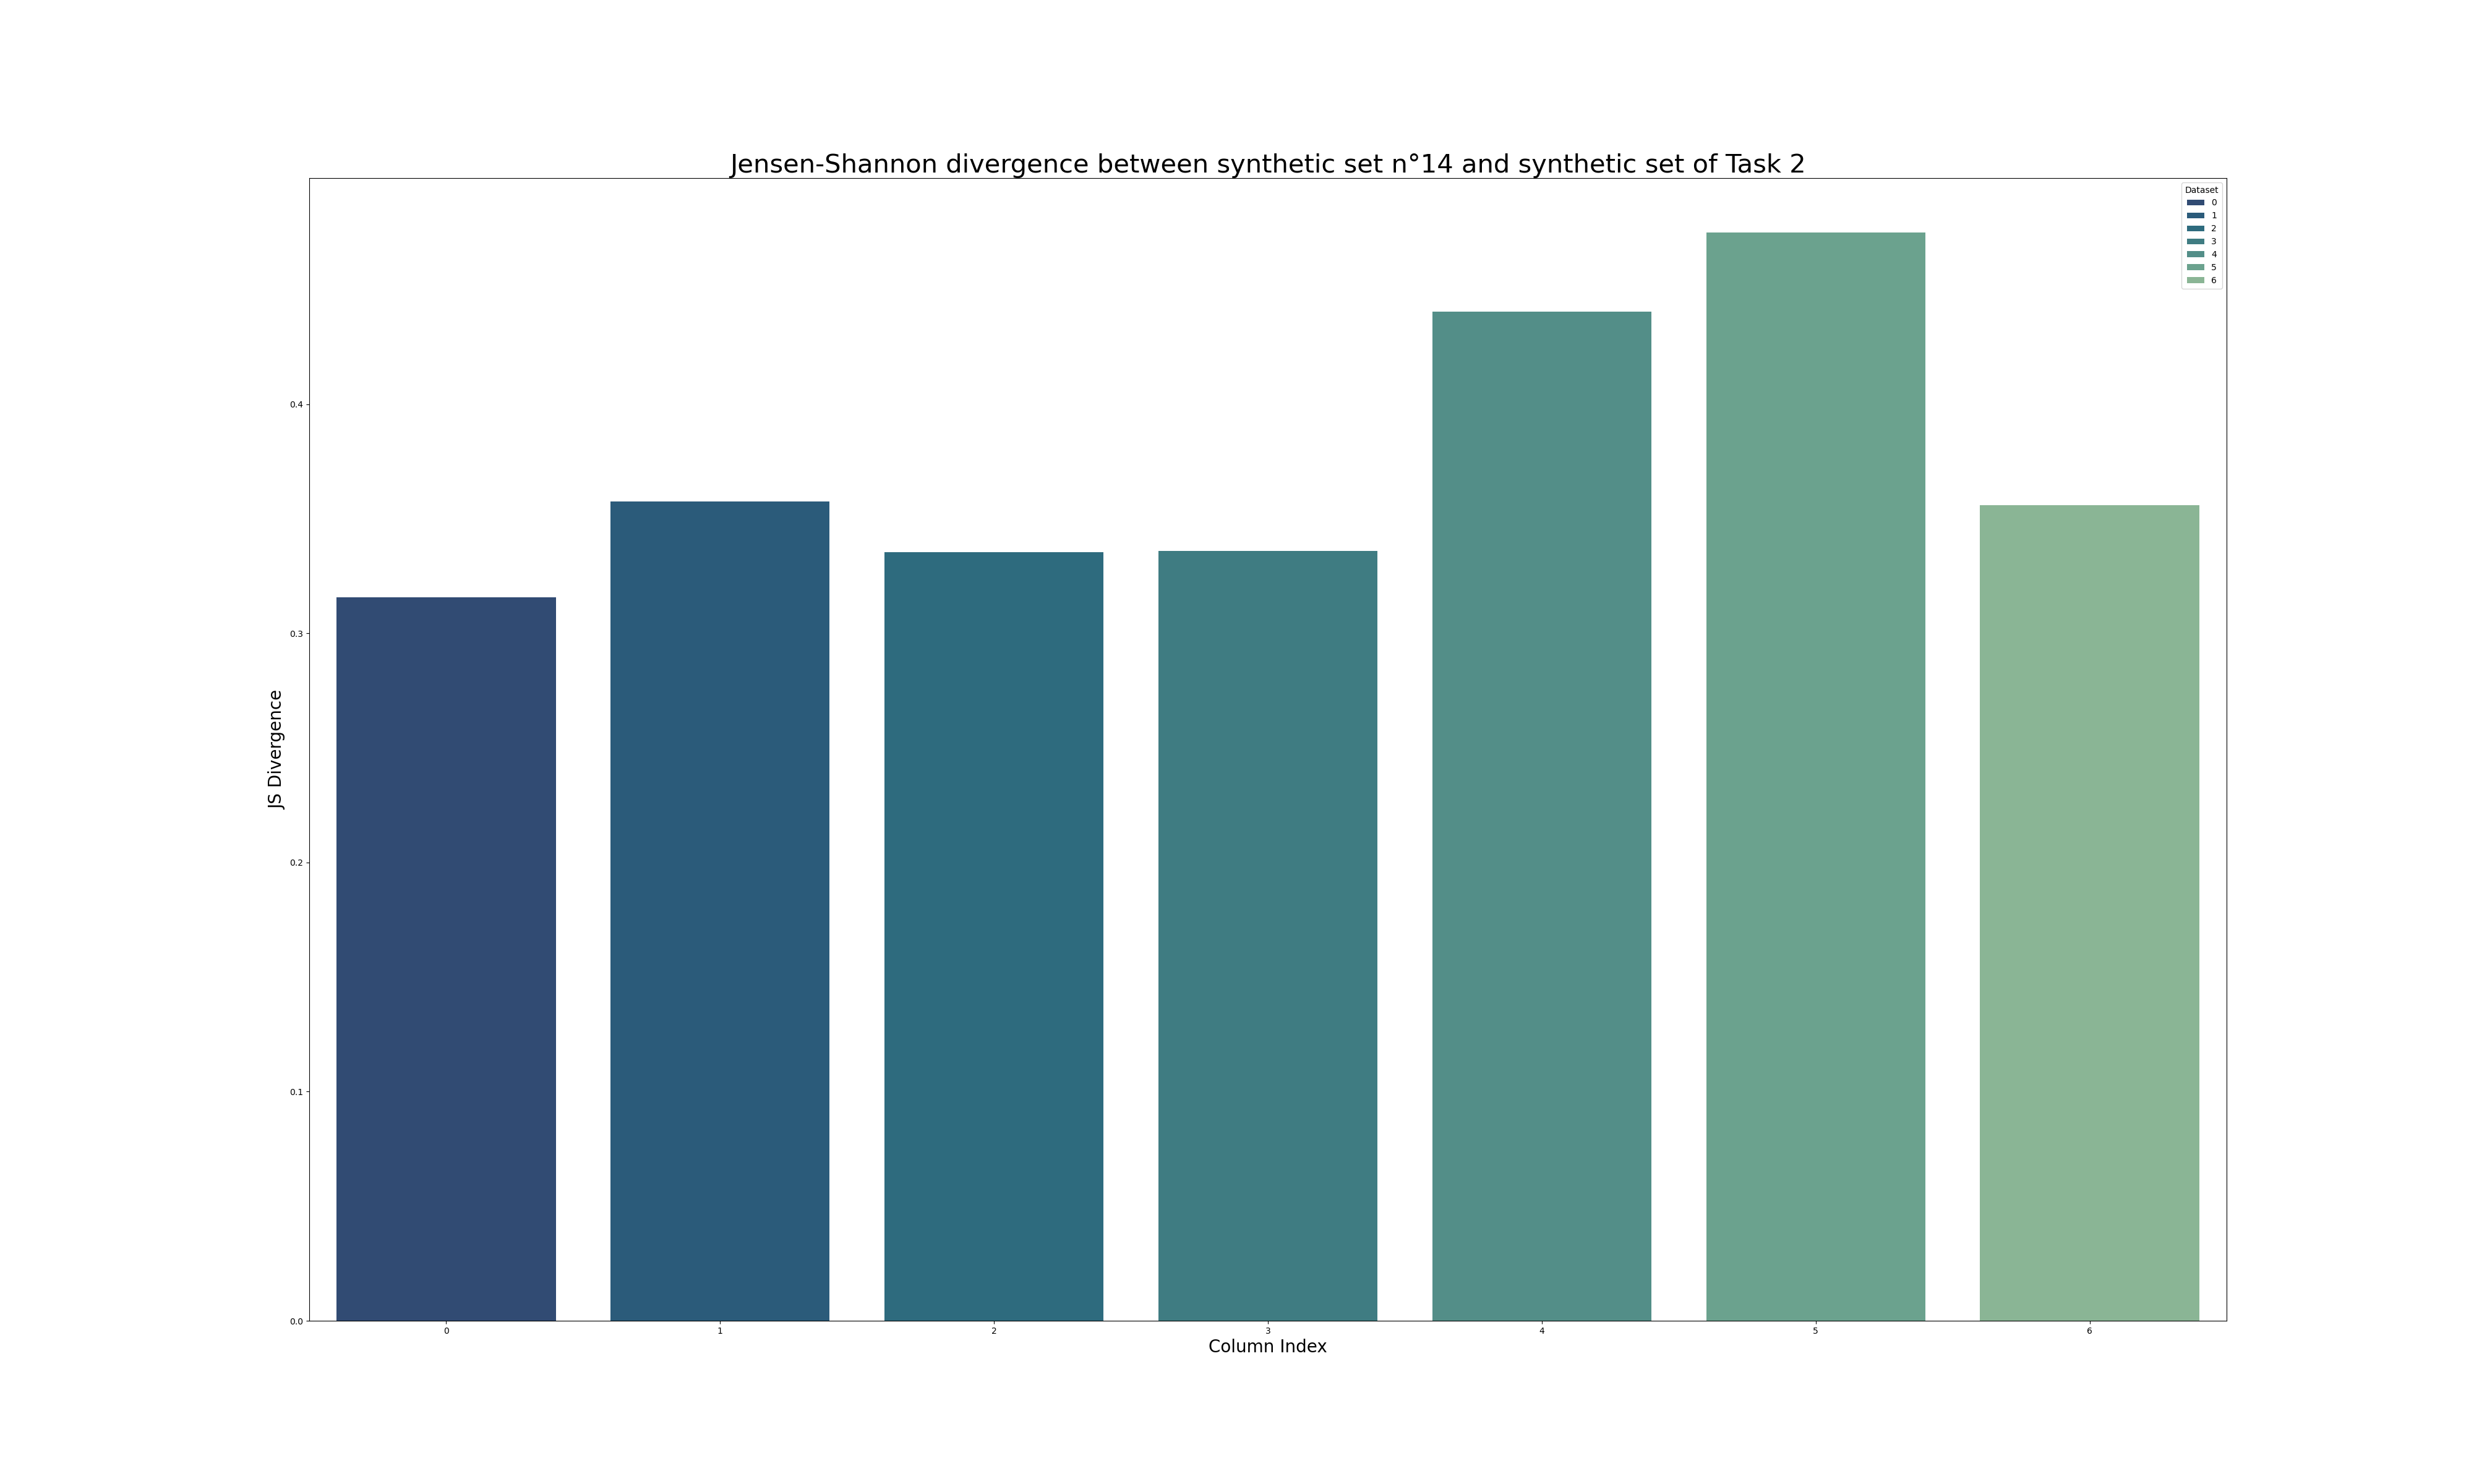
\includegraphics[width = 0.28\textwidth]{figures/Resultats/JSDivergences/14}}}\qquad
                \subfloat[]{\fbox{
                    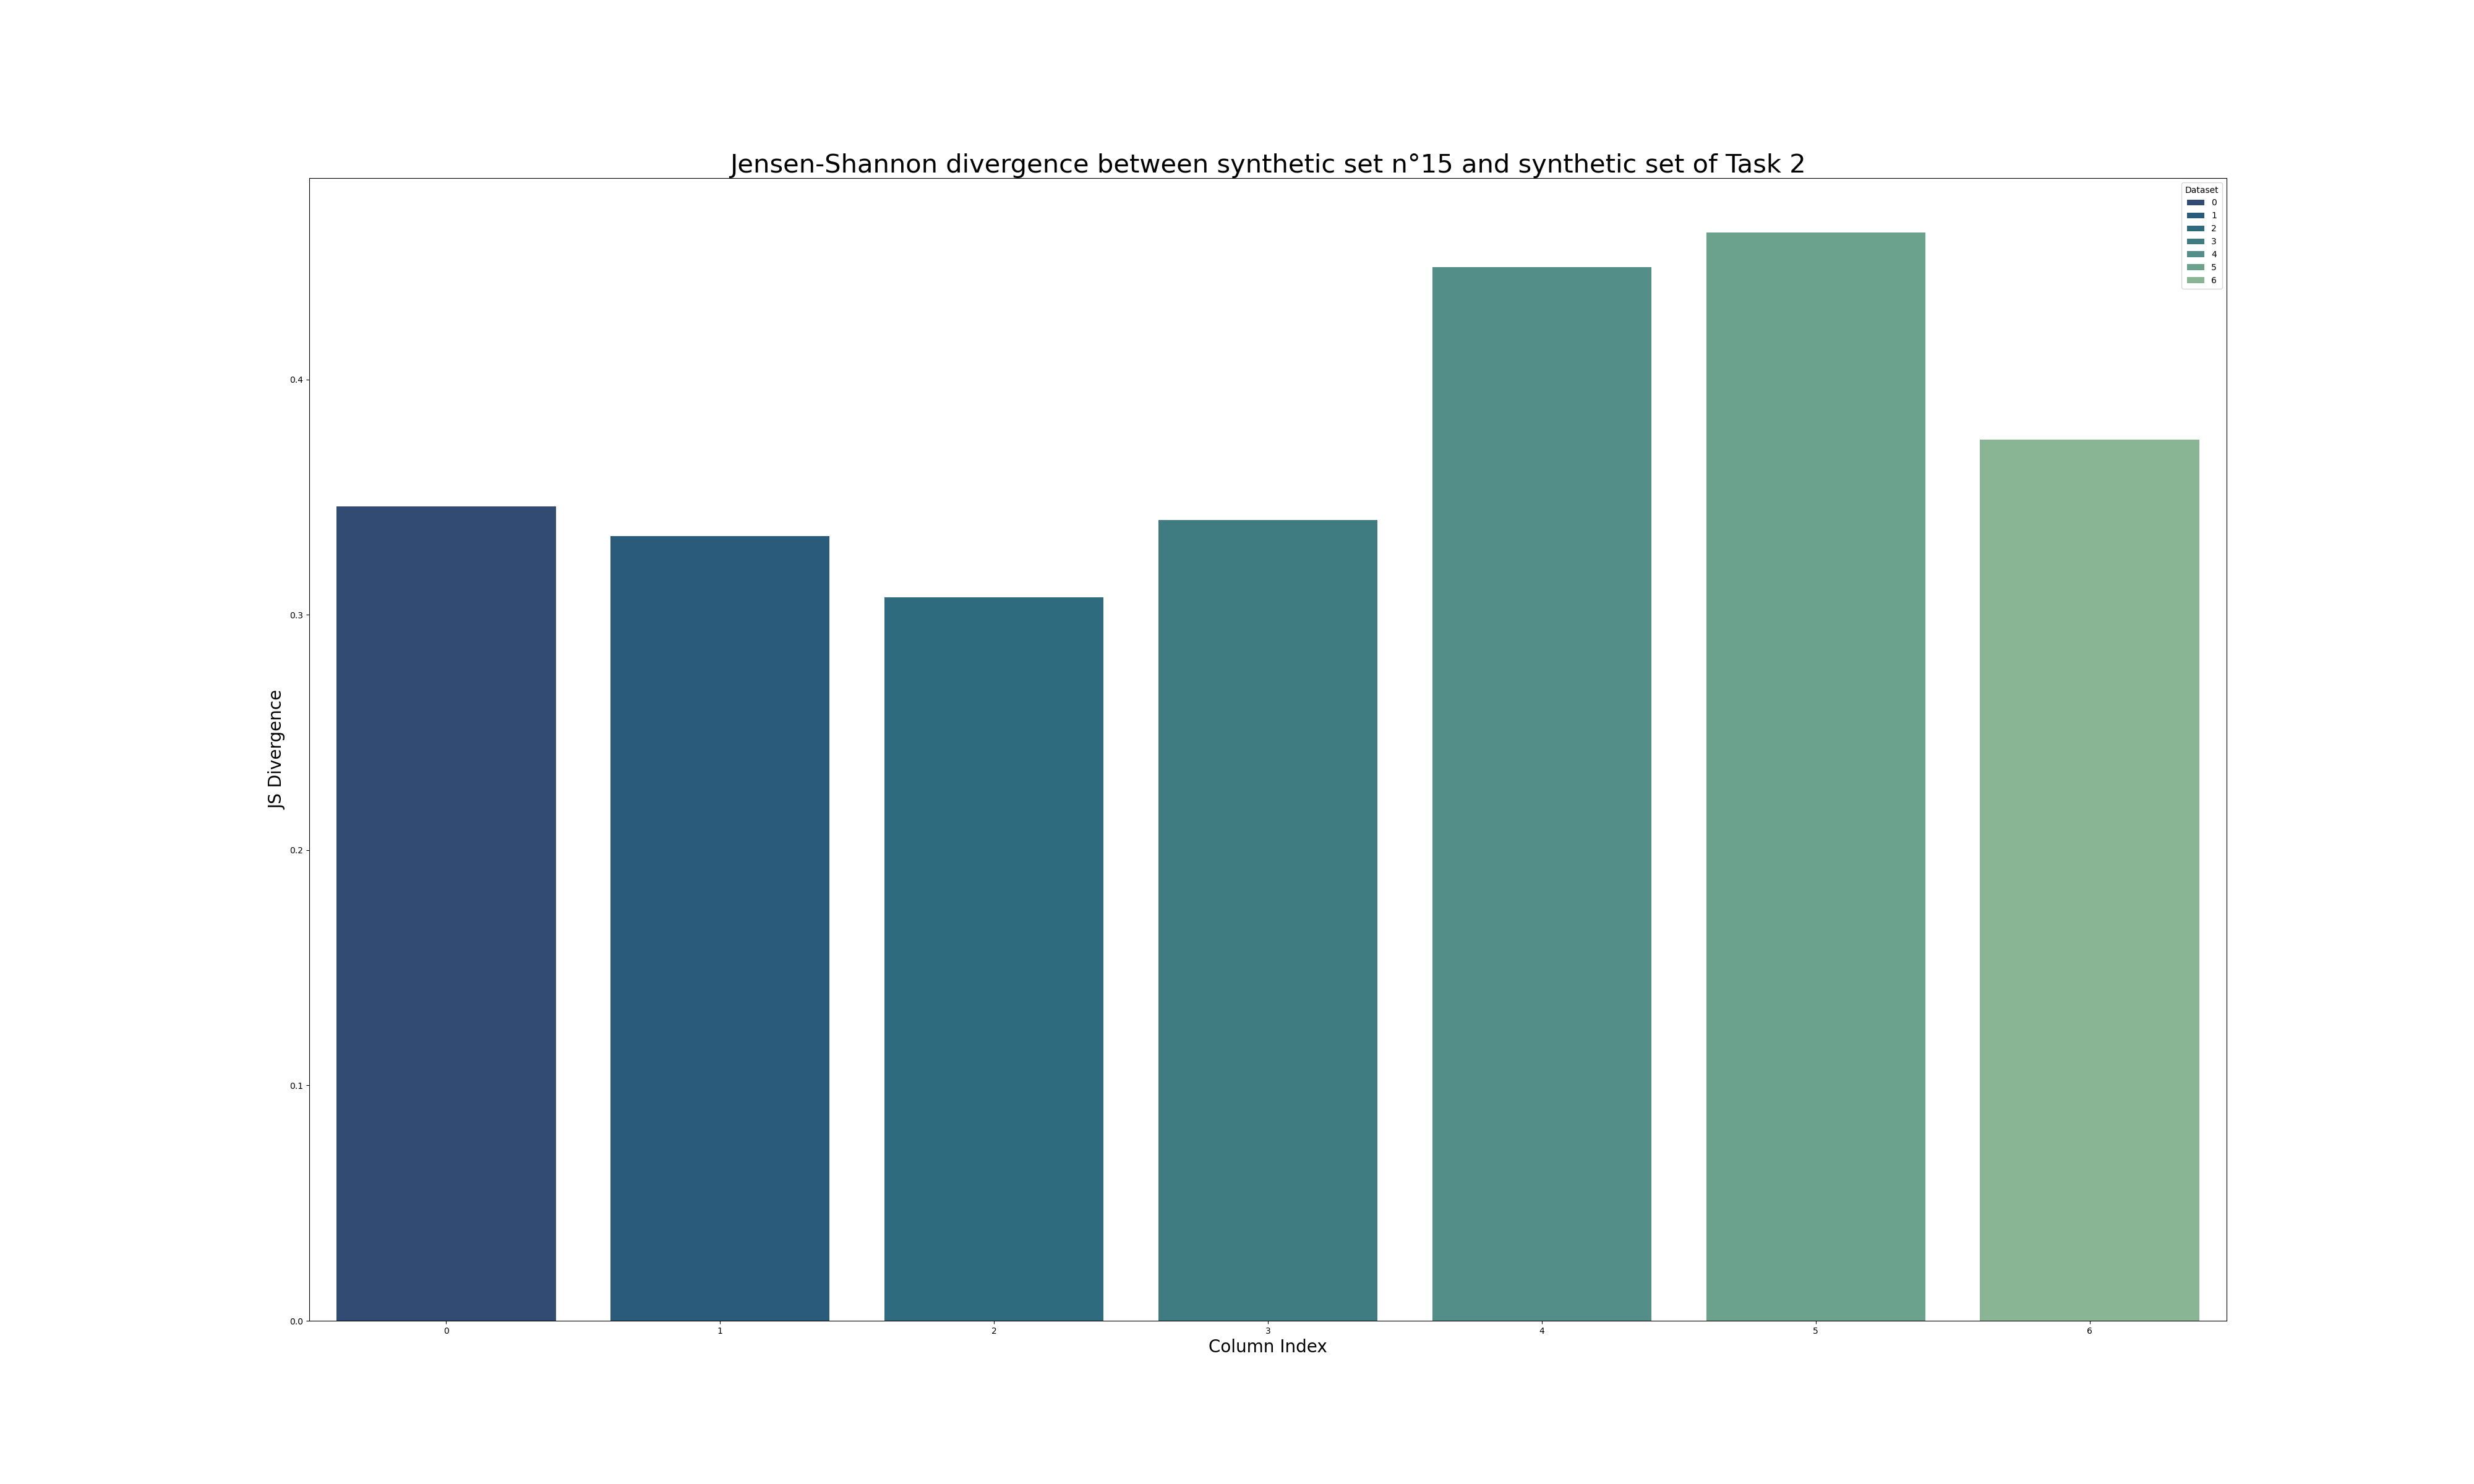
\includegraphics[width = 0.28\textwidth]{figures/Resultats/JSDivergences/15}}}\qquad
                \caption{$\mathfrak{D}\left(\mathbb{S}_{synth_{T_2}},\mathbb{S}'_{synth_i}\right)$ pour $\left(E_{T_2, \overline C, l_{30}}\right)$}
                \label{Div15S}
            \end{figure}

            \begin{figure}[H]
                \centering
                \subfloat[]{{\fbox{
                    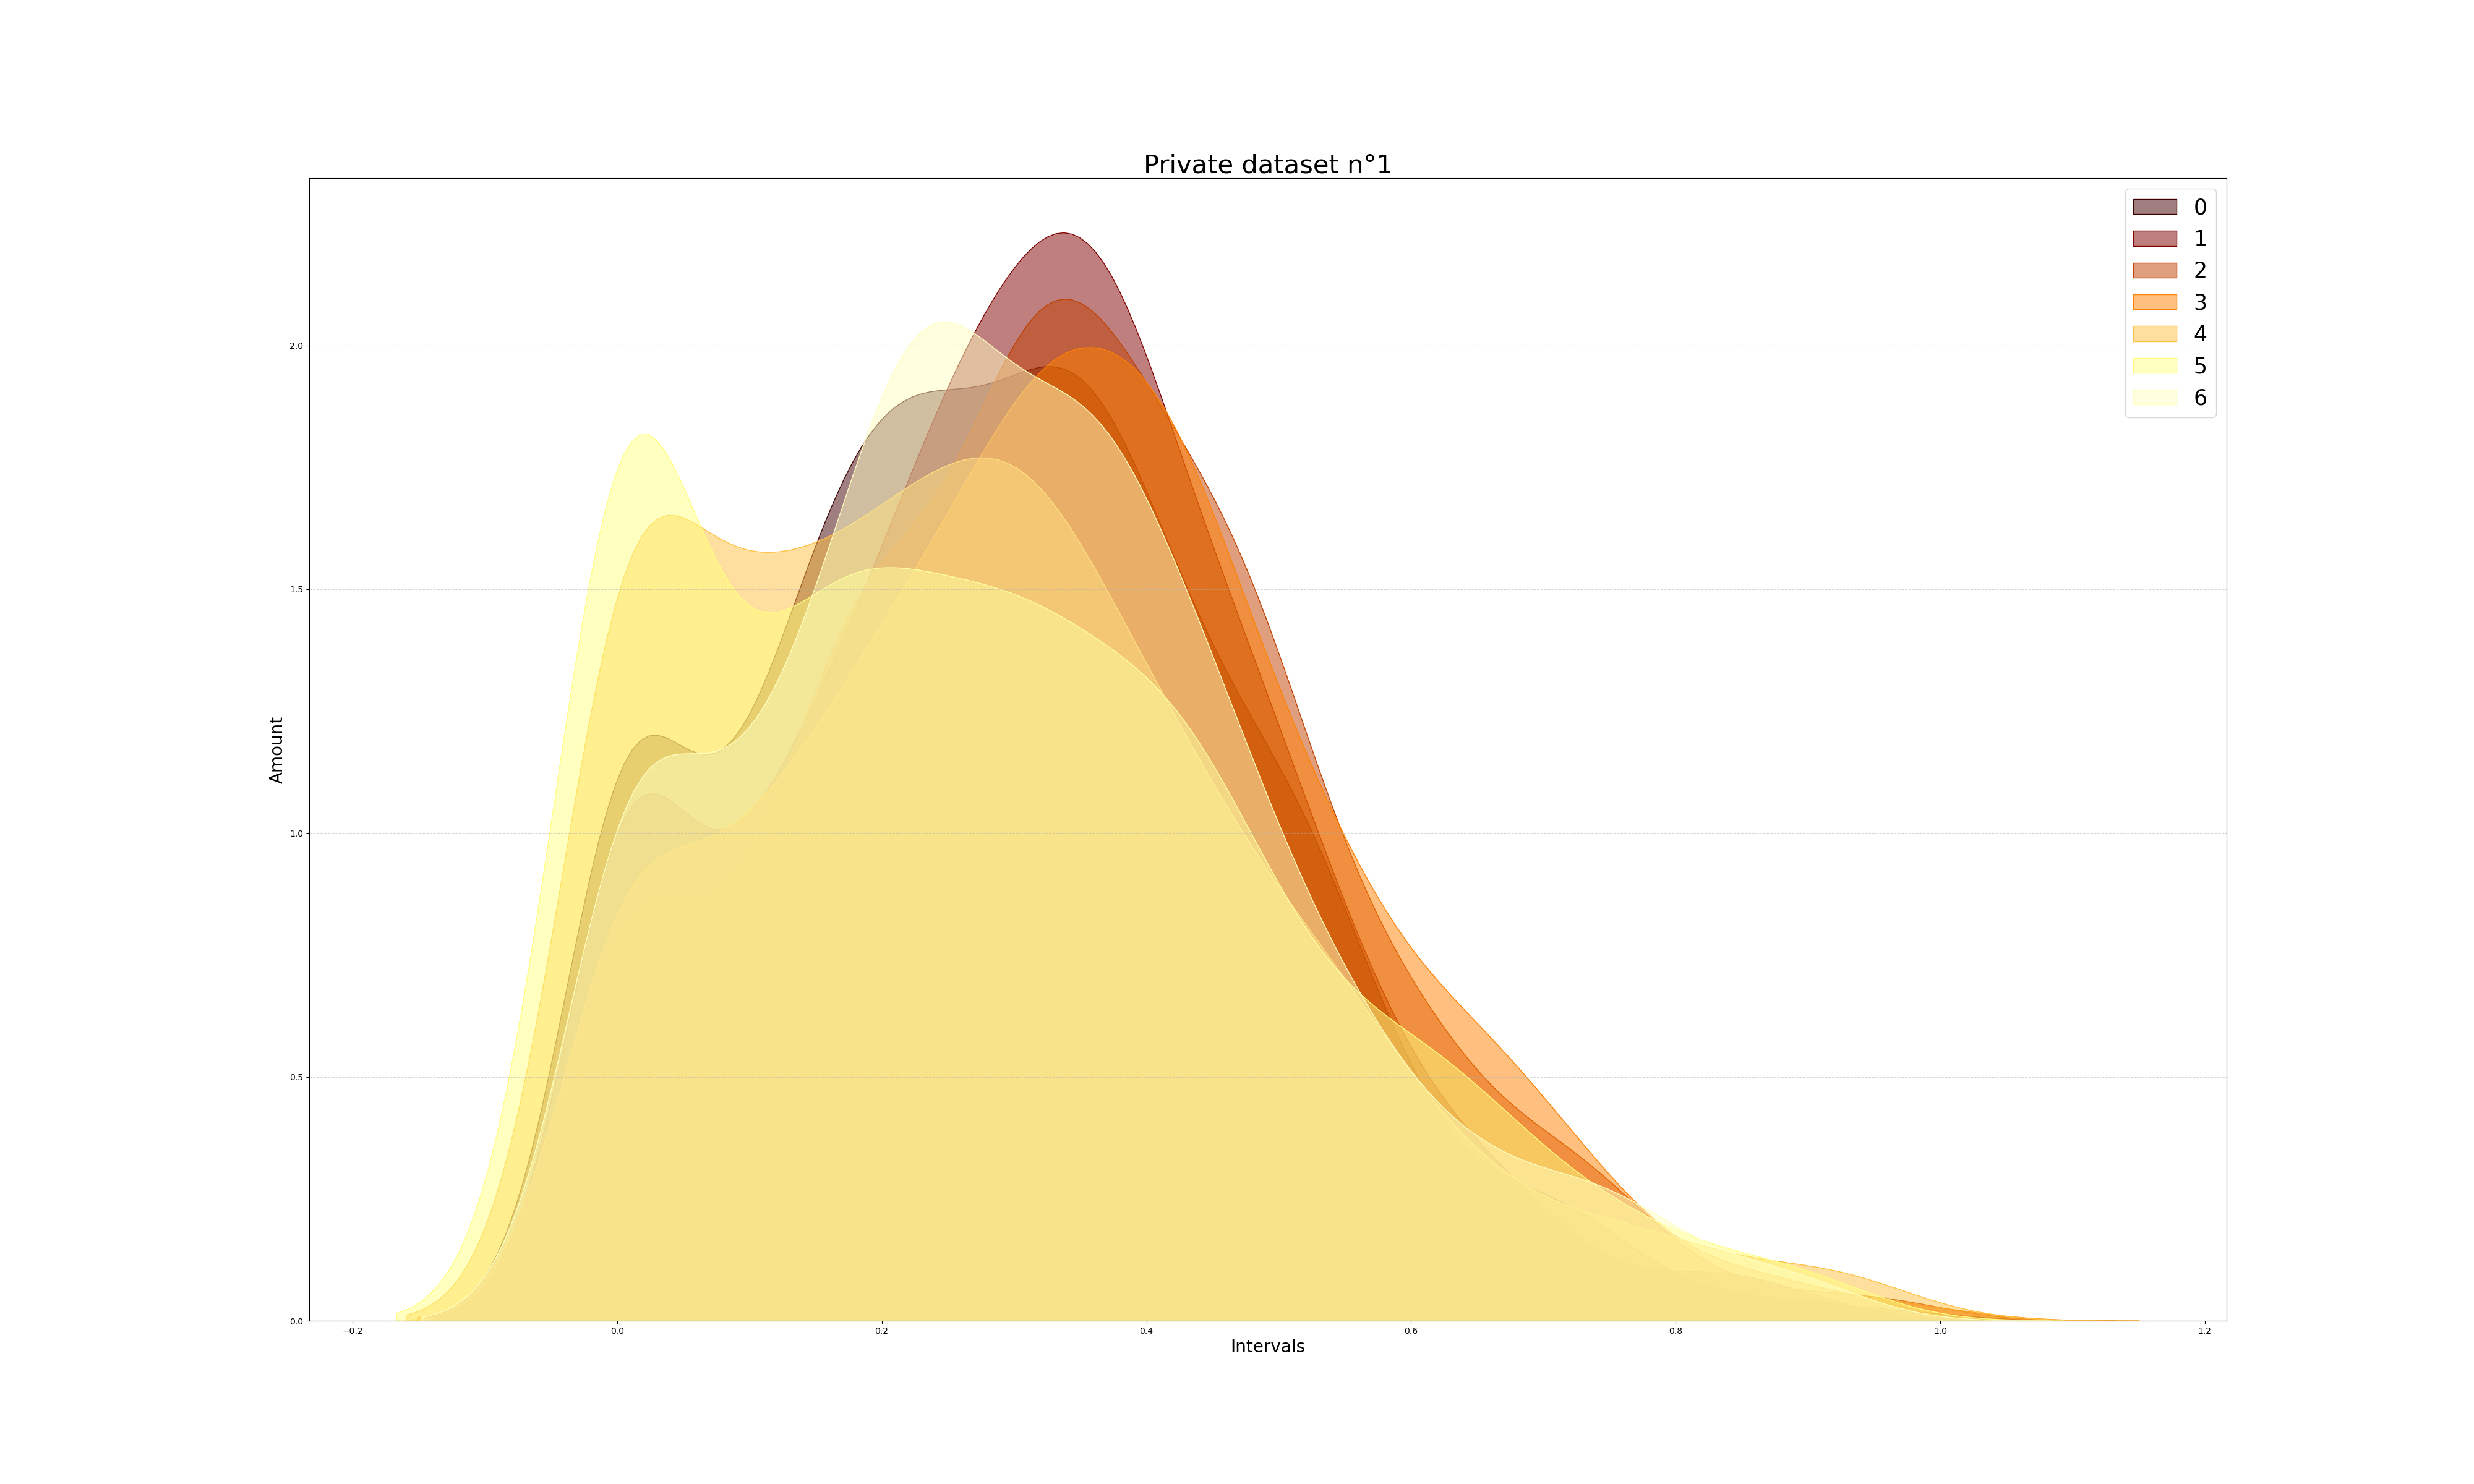
\includegraphics[width = 0.25\textwidth]{figures/Resultats/privateDS/Task 1/1}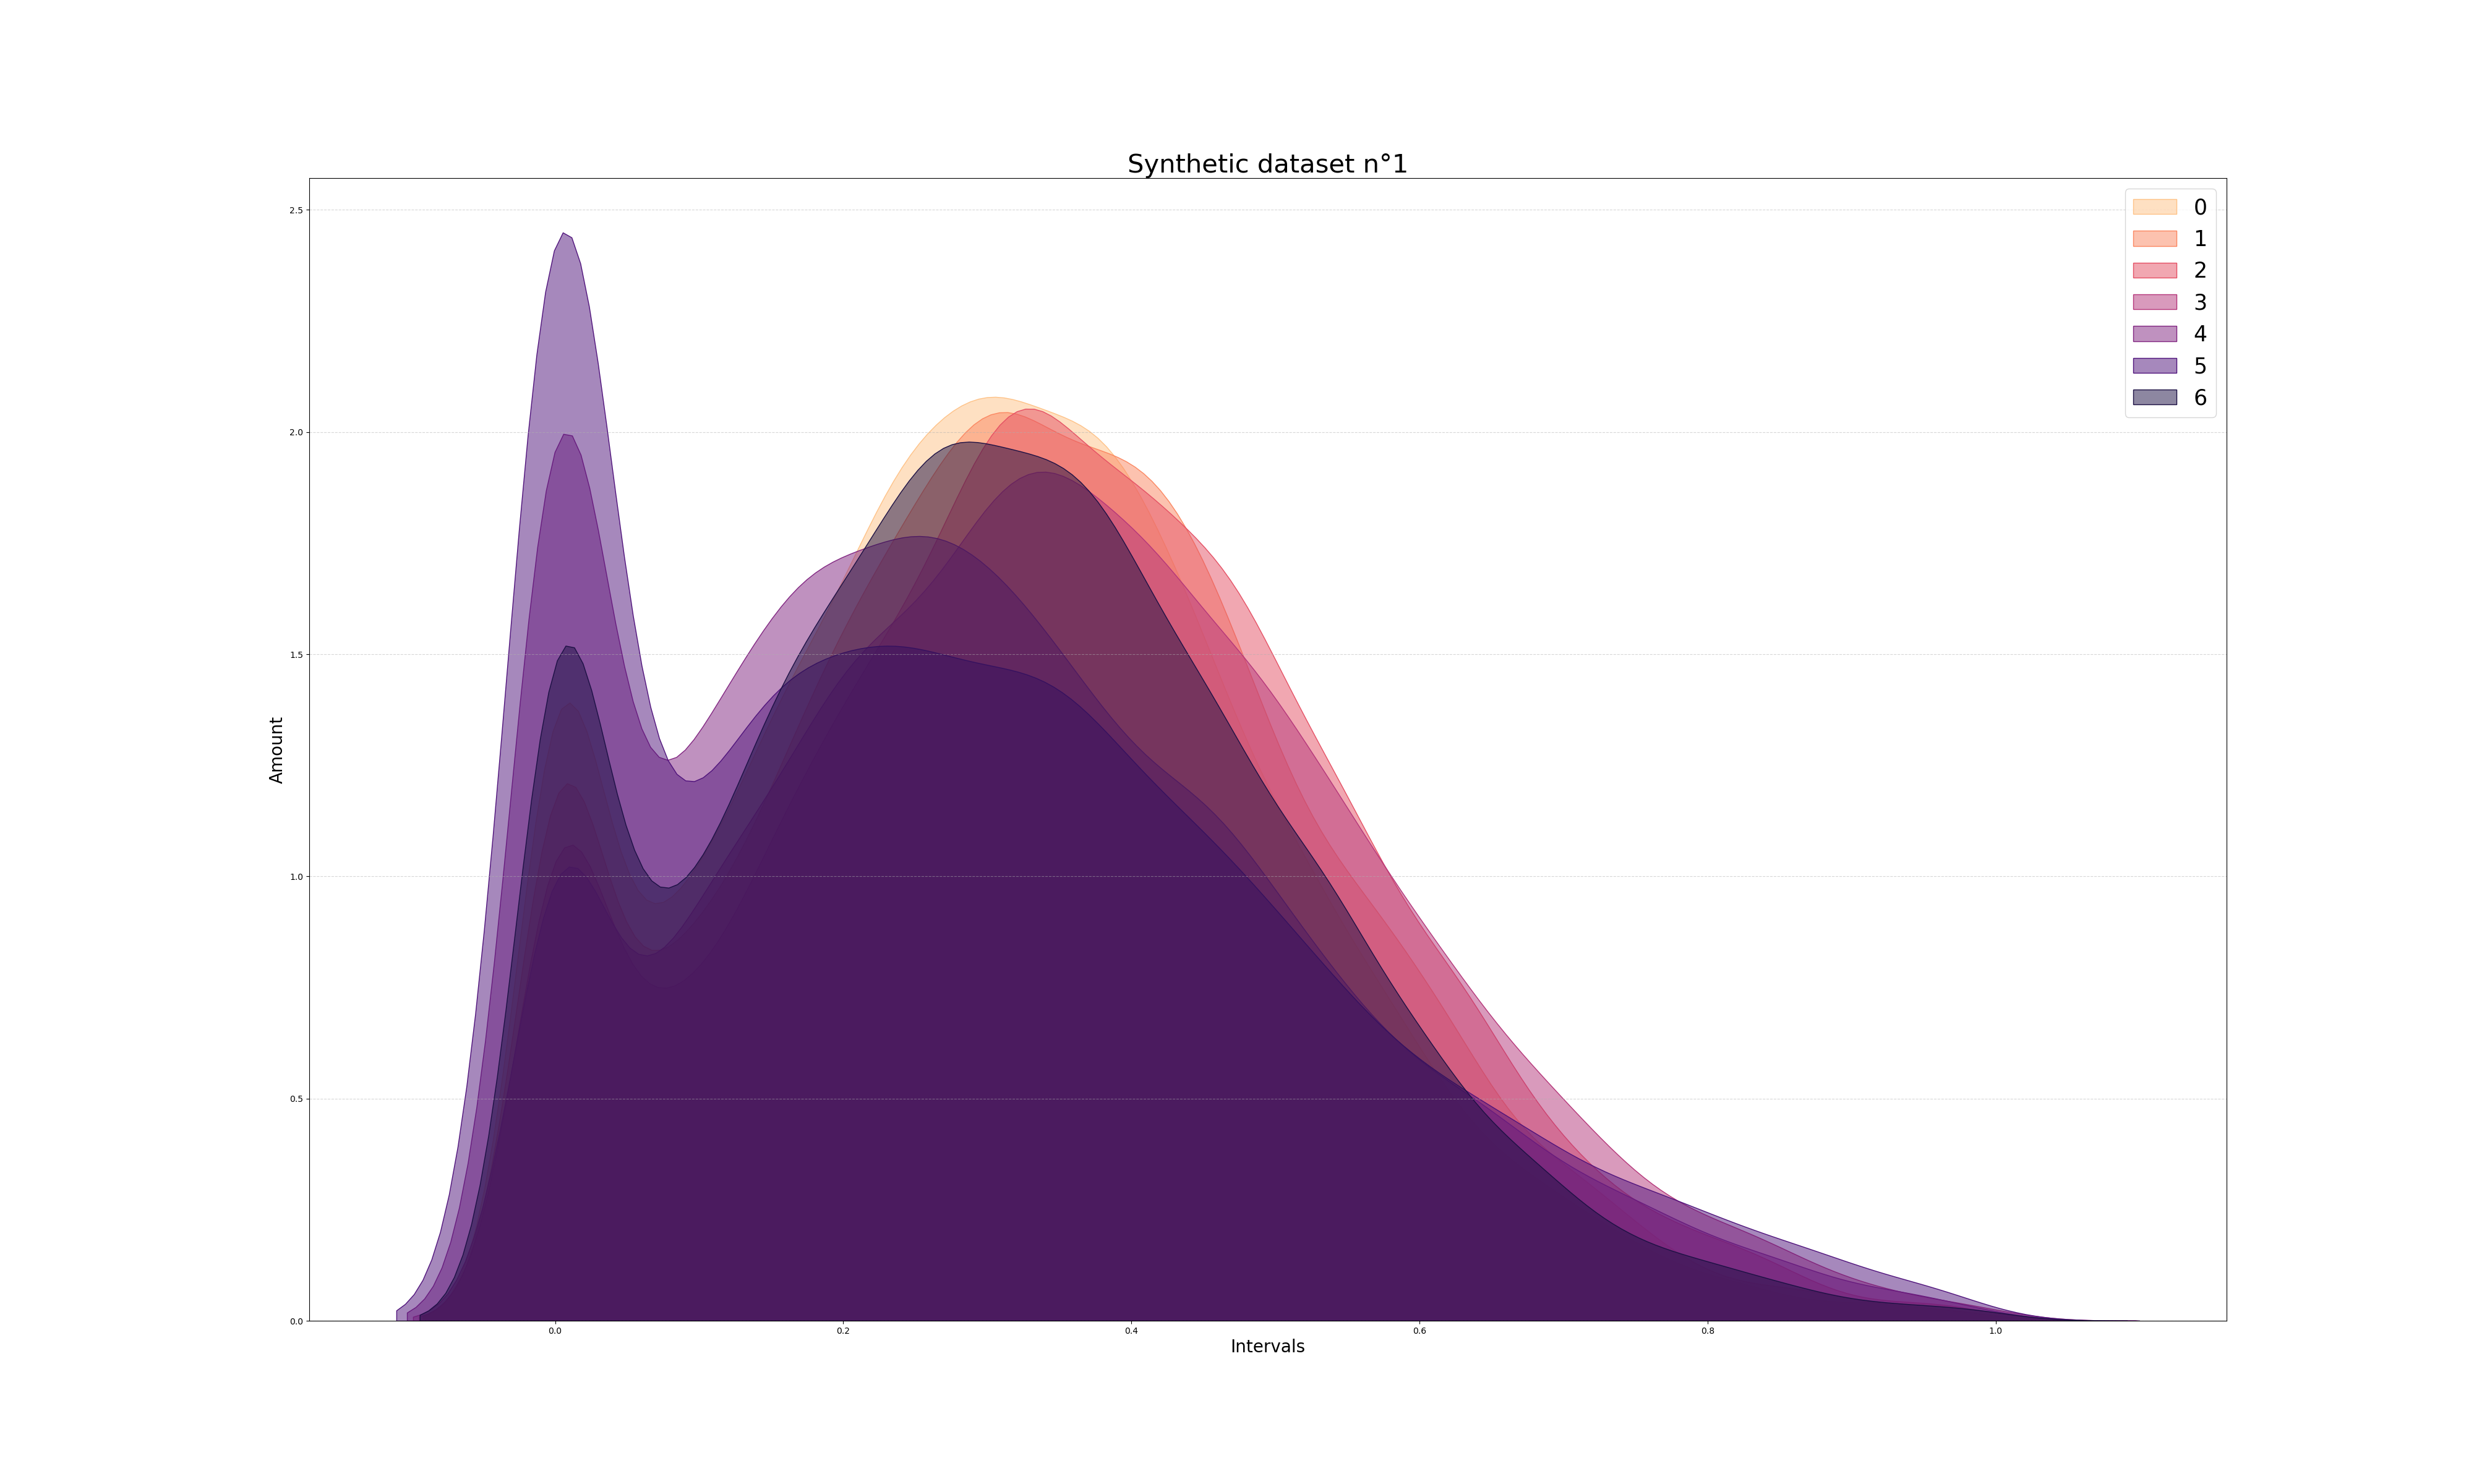
\includegraphics[width = 0.25\textwidth]{figures/Resultats/SyntheticDS/False Synthetics/Task 1/1}}}}
                \subfloat[]{{\fbox{
                    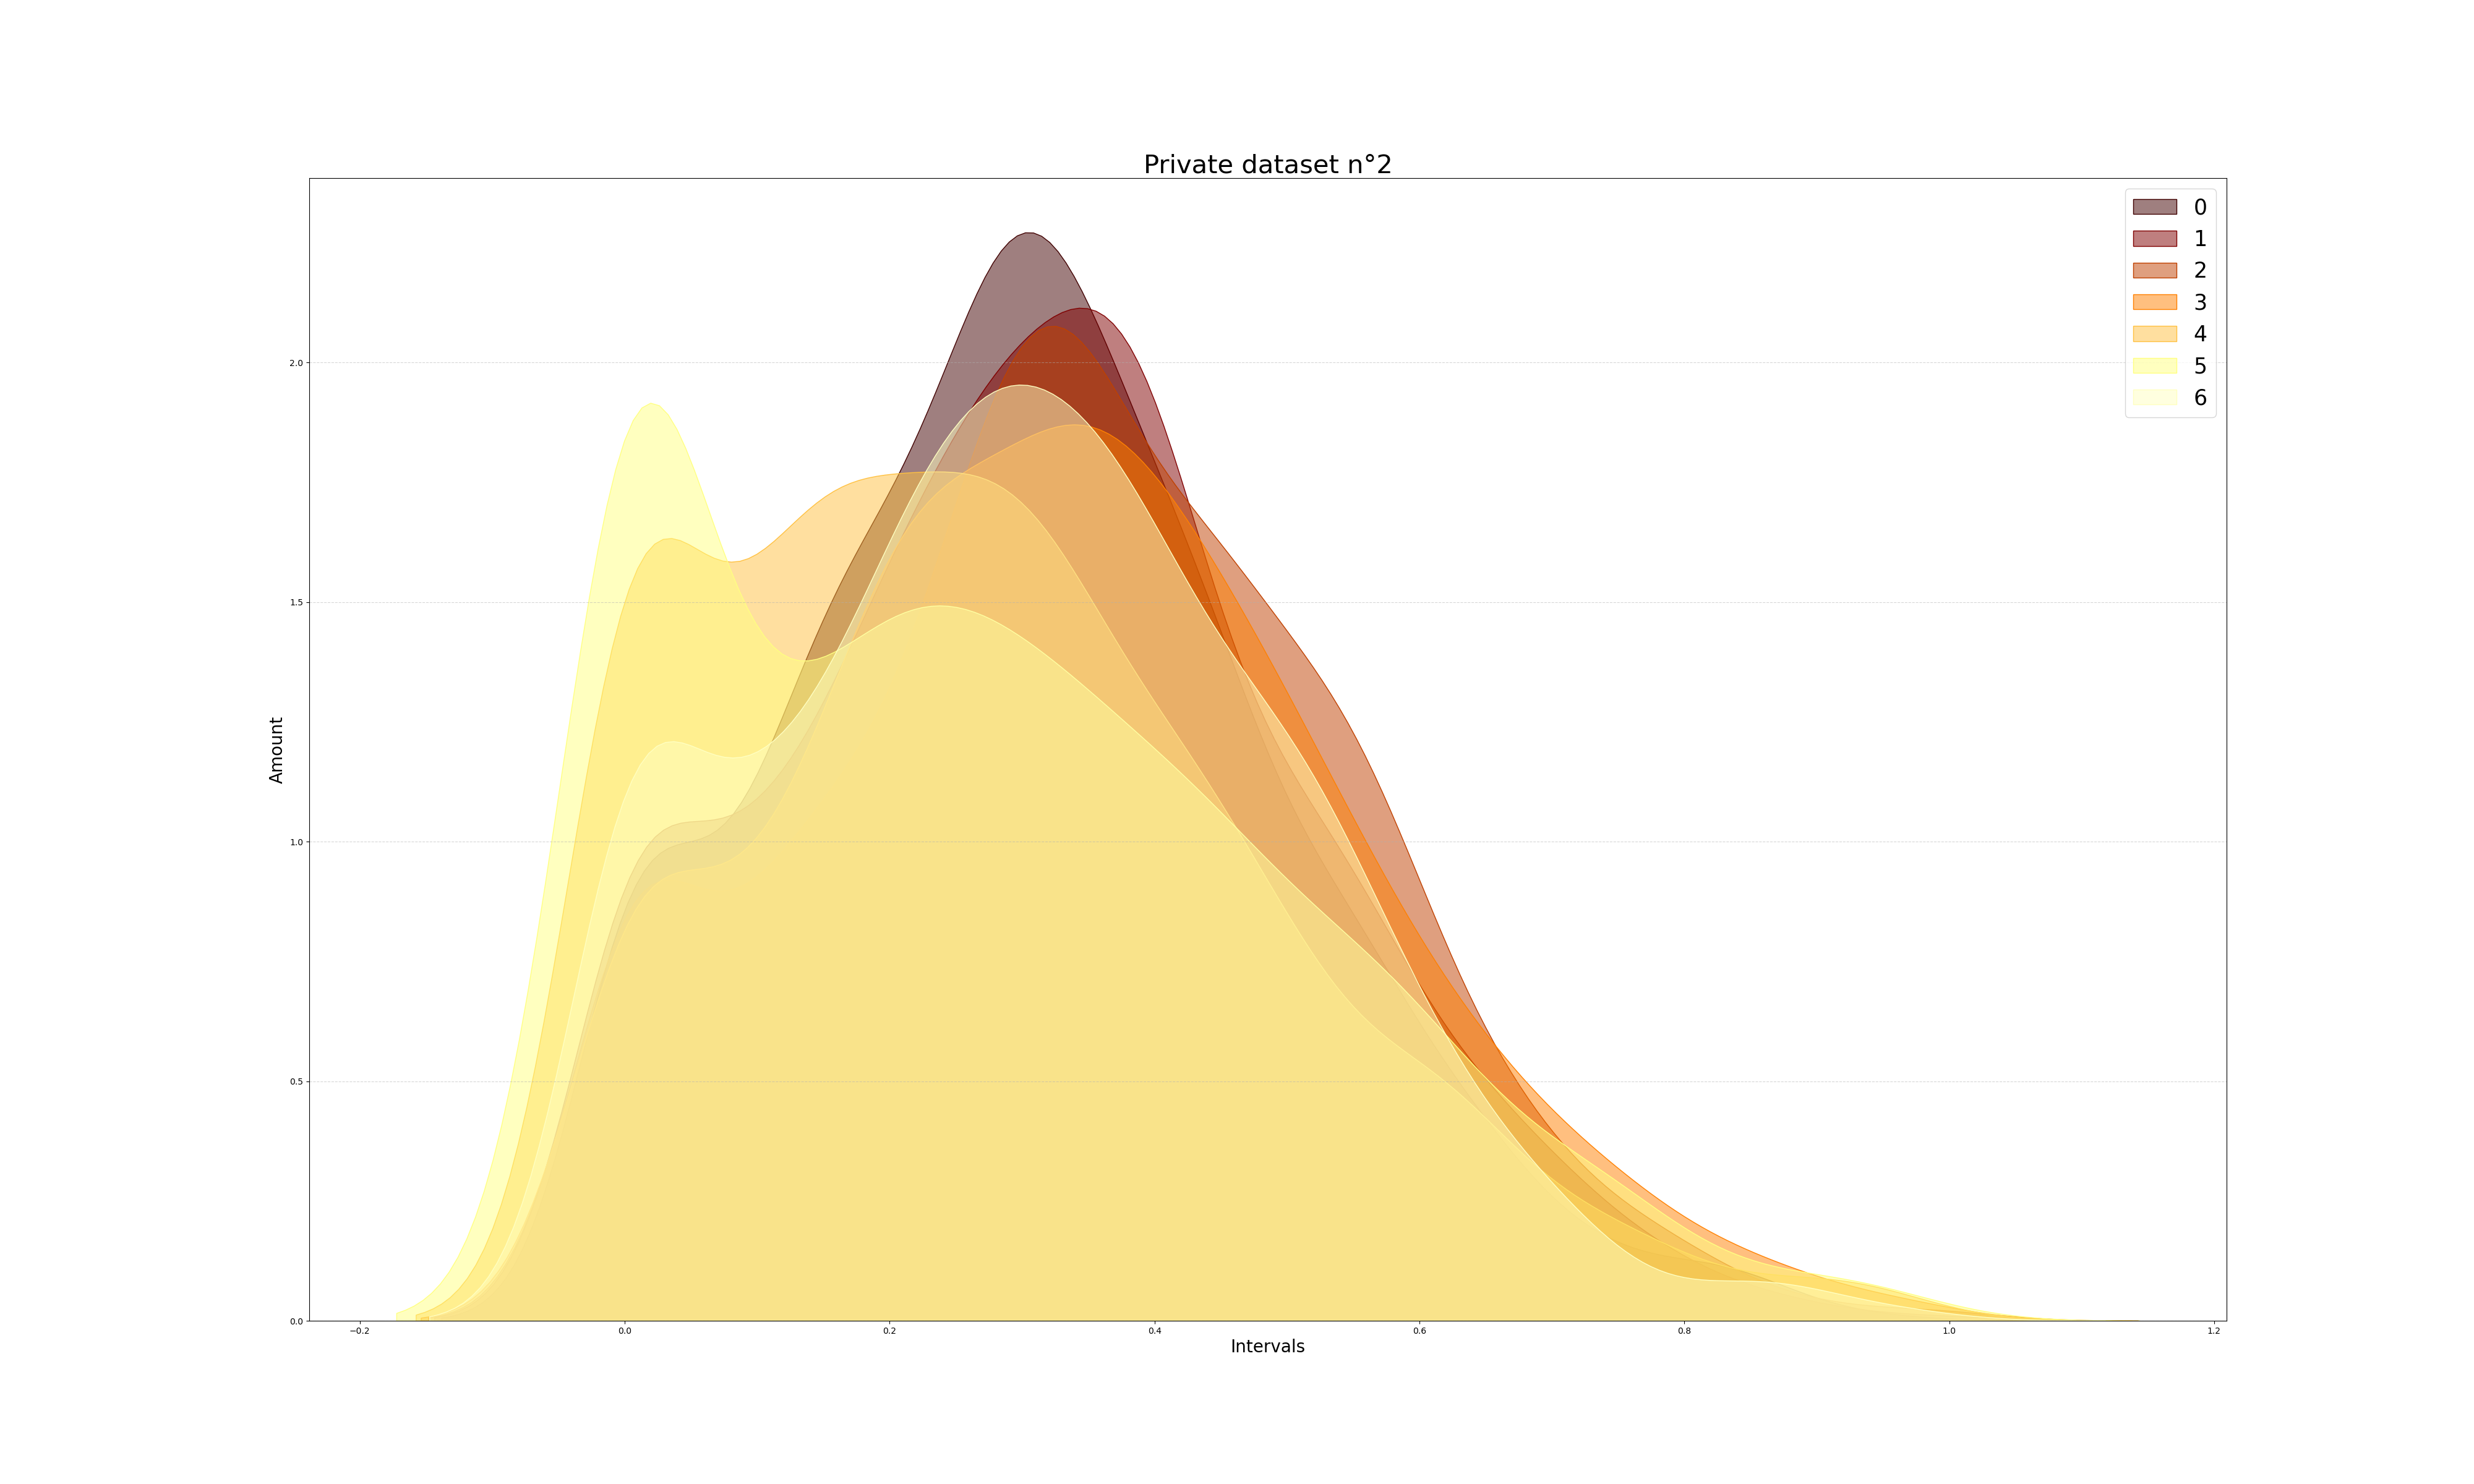
\includegraphics[width = 0.25\textwidth]{figures/Resultats/privateDS/Task 1/2}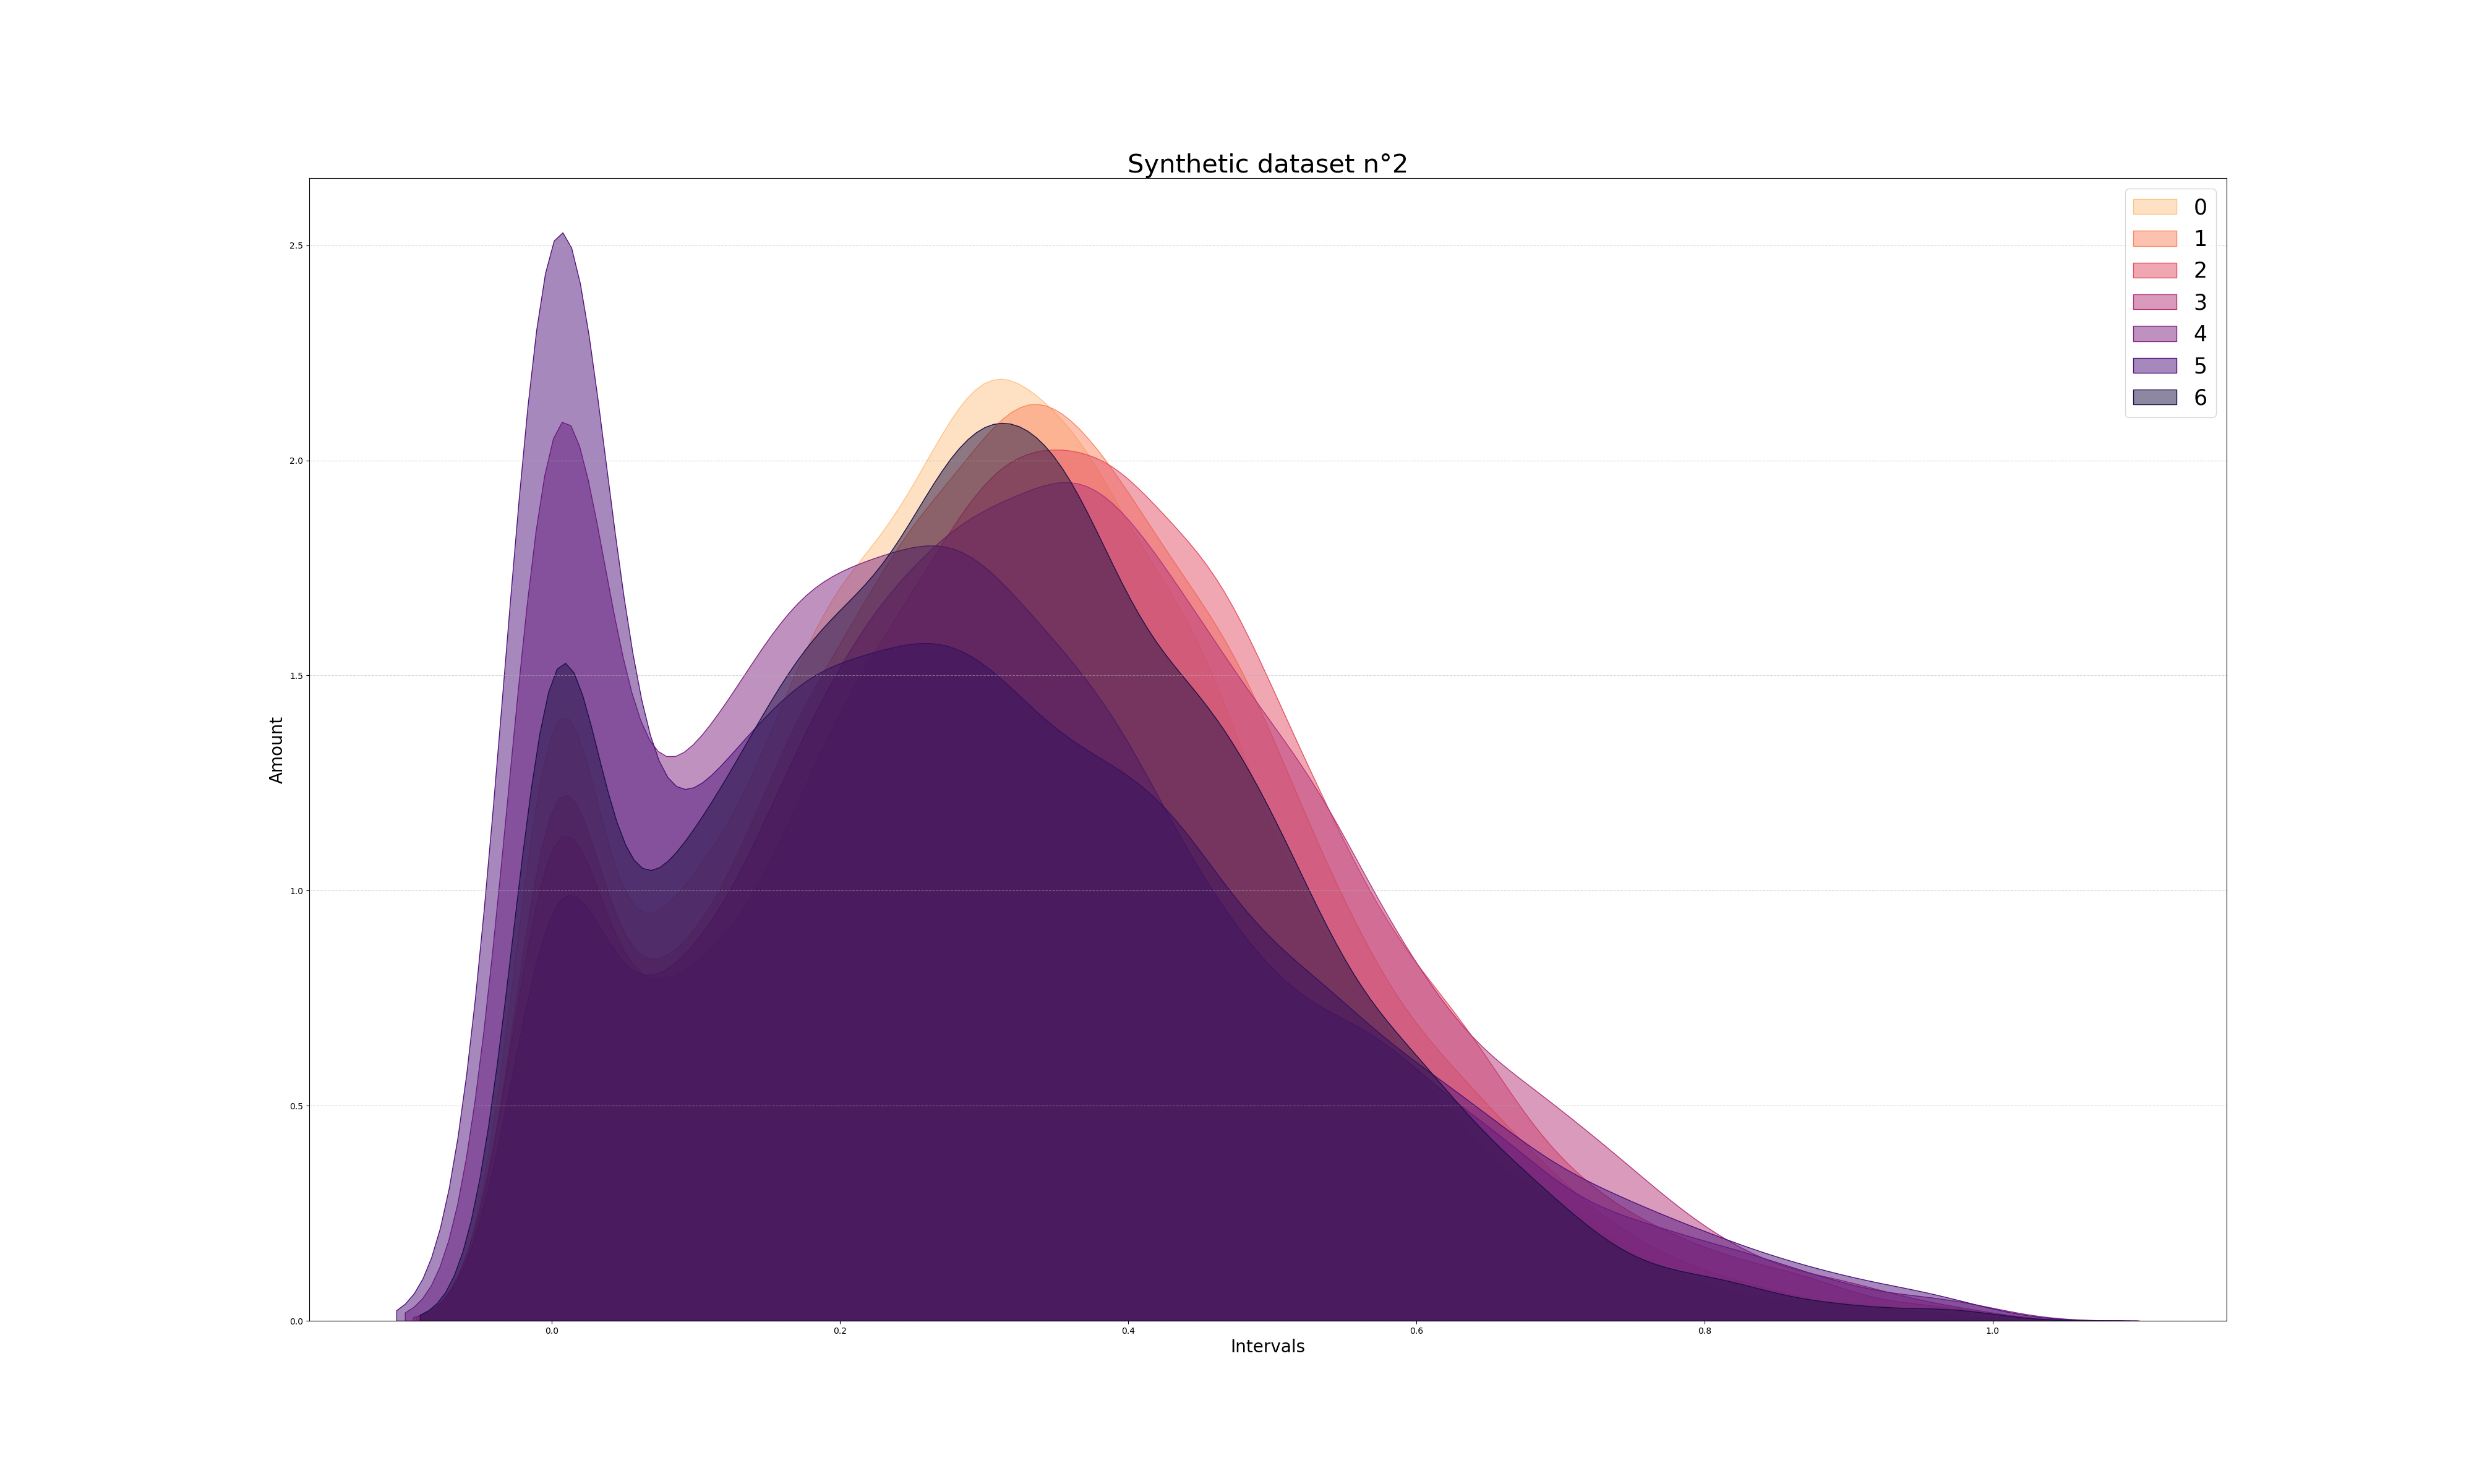
\includegraphics[width = 0.25\textwidth]{figures/Resultats/SyntheticDS/False Synthetics/Task 1/2}}}}\qquad
                \subfloat[]{{\fbox{
                    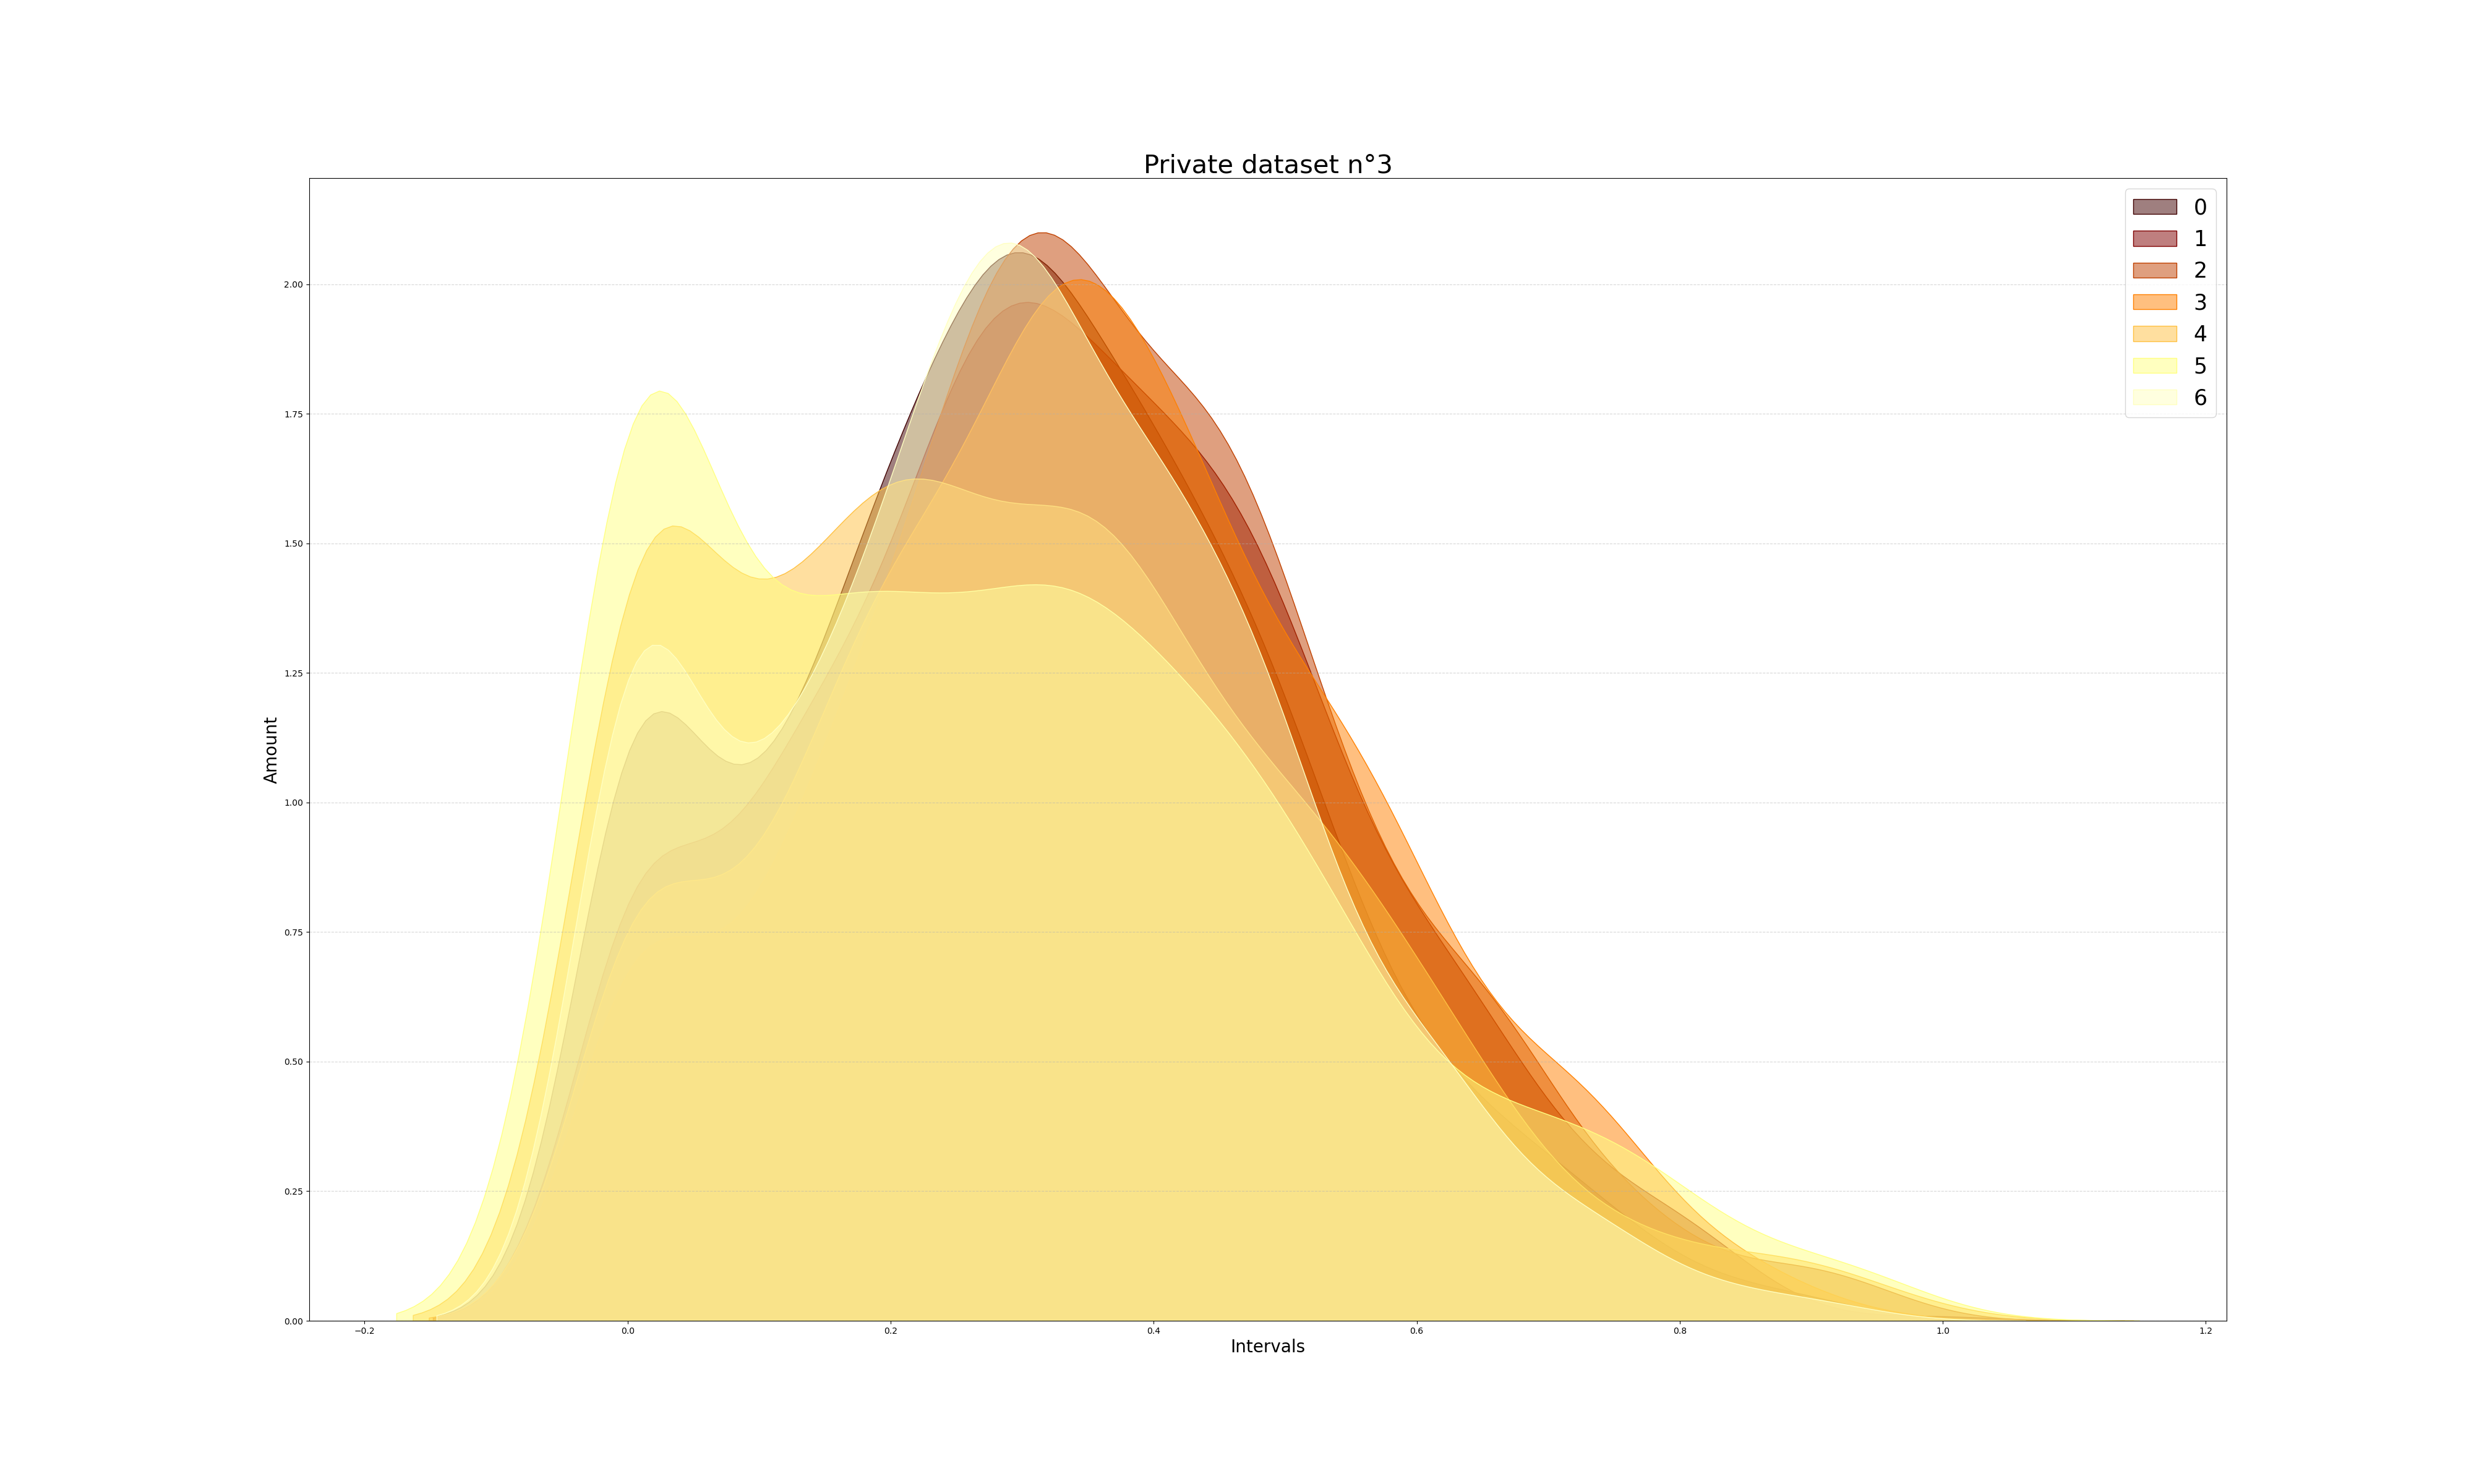
\includegraphics[width = 0.25\textwidth]{figures/Resultats/privateDS/Task 1/3}\includegraphics[width = 0.25\textwidth]{figures/Resultats/SyntheticDS/False Synthetics/Task 1/3}}}}
                \subfloat[]{{\fbox{
                    \includegraphics[width = 0.25\textwidth]{figures/Resultats/privateDS/Task 1/4}\includegraphics[width = 0.25\textwidth]{figures/Resultats/SyntheticDS/False Synthetics/Task 1/4}}}}\qquad
                \subfloat[]{{\fbox{
                    \includegraphics[width = 0.25\textwidth]{figures/Resultats/privateDS/Task 1/5}\includegraphics[width = 0.25\textwidth]{figures/Resultats/SyntheticDS/False Synthetics/Task 1/5}}}}
                \subfloat[]{{\fbox{
                    \includegraphics[width = 0.25\textwidth]{figures/Resultats/privateDS/Task 1/6}\includegraphics[width = 0.25\textwidth]{figures/Resultats/SyntheticDS/False Synthetics/Task 1/6}}}}\qquad
                \subfloat[]{{\fbox{
                    \includegraphics[width = 0.25\textwidth]{figures/Resultats/privateDS/Task 1/7}\includegraphics[width = 0.25\textwidth]{figures/Resultats/SyntheticDS/False Synthetics/Task 1/7}}}}
                \subfloat[]{{\fbox{
                    \includegraphics[width = 0.25\textwidth]{figures/Resultats/privateDS/Task 1/8}\includegraphics[width = 0.25\textwidth]{figures/Resultats/SyntheticDS/False Synthetics/Task 1/8}}}}\qquad
                \subfloat[]{{\fbox{
                    \includegraphics[width = 0.25\textwidth]{figures/Resultats/privateDS/Task 1/9}\includegraphics[width = 0.25\textwidth]{figures/Resultats/SyntheticDS/False Synthetics/Task 1/9}}}}
                \subfloat[]{{\fbox{
                    \includegraphics[width = 0.25\textwidth]{figures/Resultats/privateDS/Task 1/10}\includegraphics[width = 0.25\textwidth]{figures/Resultats/SyntheticDS/False Synthetics/Task 1/10}}}}\qquad
                \caption{
                    $\mathfrak H\left( \mathbb{S}'_{Etr_{i_{T_{1}}}}, \mathbb{S}'_{Synth_{i_{T_{1}}}}\right) \Bigm \lvert \left(E_{T_1, \overline C, l_{200}}\right)$}
            \end{figure}

    \newpage\section{Regroupement d'un nombre important de datasets et nettoyage des données
        $\left(E_{T_2, \overline C, l_{100}}\right)$}\label{nettoyage}

        Les résultats précédents montrent que l'augmentation de $l\left( \mathbb S'_{priv} \right)$ est inefficace, \textit{(voire contre-productive)}
        au-dela d'un certain seuil. On reprend alors les équations \ref{eq:Eq1} et \ref{eq:Eq2}
        et on cherche à construire $\mathbb S'_{priv}$ avec des considérations plus fines.

        \subsection{Métriques de comparaison pour piloter le nettoyage}

            En substance, il est aisé d'émettre la réflexion suivante : "Si les datasets
            synthétiques générés par nos modèles sont similaires aux datasets synthétiques
            donnés pour la compétition, alors on peut donner les données d'entraînement des
            modèles en entrée d'un classifieur et espérer raisonnablement qu'il soit adapté à
            l'attaque de $\mathcal G$". En revanche, il est beaucoup plus difficile de vérifier
            la première partie de cette assertion.

            Pour ce faire, on peut assimiler les séries temporelles à une distribution
            statistique \textit{(à l'instar de notre procédé pour visualiser les données)}, et
            les normaliser pour approximer une distribution probabiliste. Ainsi, il est possible
            d'utiliser un certain nombre de métriques pour apprécier les similitudes entre ces
            distributions. Deux d'entre elles ont été retenues : la divergence de
            Kullback-Leibler (\cite{wikiKLD}) et la divergence de Jensen-Shannon (\cite{wikiJSD}).

            Leurs formules sont rappelées ci-dessous.

            \begin{equation}\label{eq:Eq3}
                \mathfrak D \left( P || Q \right) = \sum_{x\in X} P(x)\log \frac{P(x)}{Q(x)}
            \end{equation}\myequations{Divergence de Divergence de Kullback-Leibler entre deux distributions de probabilités}

            \begin{equation}\label{eq:Eq4}
                \mathfrak{JSD}\left( P||Q \right) = \frac12 \mathfrak D\left( P||M \right) +\frac
            12 \mathfrak D \left( Q || M \right),\Bigm \lvert M=\frac12 \left( P+Q \right)
            \end{equation}\myequations{Divergence de Divergence de Jensen–Shannon entre deux distributions de probabilités}


            \begin{tcolorbox}[colback=linkborder_Color!5!white,colframe=linkborder_Color!75!black]
                La divergence de Jensen-Shannon possède des propriétés de symétrie et de finitude
                des valeurs qui rendent son utilisation plus facile que la divergence de
                Kullback-Leibler. C'est donc celle-ci que l'on utilisera et cherchera à minimiser \textit{(une divergence nulle signifiant une exactitude entre les deux ensembles)}.
            \end{tcolorbox}.

            On notera $\mathfrak D$ la divergence de Jensen-Shannon par la suite. Comme un
            dataset est décomposé en 7 distributions, le calcul d'une divergence pour un dataset
            donne en sortie un 7-uplet. On peut donc visualiser la divergence d'une expérience
            entière \textit{(ie un grand nombre de datasets)} avec la même représentation que
            précédemment :

            \begin{figure}[H]
                \centering
                \fbox{
                    \includegraphics[width = 0.8\textwidth]{figures/Resultats/JSDivergences/JSD for 50 sets}}
                \caption{$\mathfrak{D}\left(\mathbb{S}_{synth_{T_2}},\mathbb{S}'_{synth_i}\right)$ pour $\left(E_{T_2, \overline C, l_{100}}\right)$}
            \end{figure}

            \begin{figure}[H]
                \centering
                \fbox{
                    \includegraphics[width = 0.8\textwidth]{figures/Resultats/JSDivergences/Task 1/JSD for 10 sets}}
                \caption{$\mathfrak{D}\left(\mathbb{S}_{synth_{T_1}},\mathbb{S}'_{synth_i}\right)$ pour $\left(E_{T_1, \overline C, l_{200}}\right)$}
            \end{figure}
        \subsection{Limite imposée par le temps de calcul}

            Un résultat inattendu de l'étude est la durée de calcul non négligeable qu'engendre
            une augmentation de $l\left(\mathbb{S}'_{priv}\right)$. Ainsi, quand $l\left( \mathbb{S}'_{priv} \right) \approx 10^5$,
            $\mathcal C \left( \mathbb C \right) \approx 48h$. Un rapide relevé des temps de
            calcul laisse supposer une complexité quadratique pour les méthodes de
            classification utilisée, ce qui empêche de toute manière une classification
            basée seulement sur la quantité de données générées.

           \begin{figure}[H]
                \centering\fbox{
                    \includegraphics[width = 0.5\textwidth]{figures/Resultats/time/lengthVStime}}
                \caption{Durée totale d'une classification en fonction de $l\left(\mathbb S_{etr}\right)$}
            \end{figure}
        \newpage\subsection{Nettoyage de $\mathbb{S}'_{priv_i}$}
            Il s'agit de la partie la plus délicate de l'étude. En effet, on a réussi à
            générer de nombreux $\mathbb{S}'_{priv_i}$
            \footnote{Cette partie est d'ailleurs semi-automatisée avec un script \texttt{Bash} écrit par l'équipe} et à apprécier la divergence
            des données générées avec les données générées par le modèle attaqué, mais rien
            n'est à ce stade envisagé pour diminuer cette divergence.

            La principale difficulté est que comme vu plus haut \textit{(\ref{divNonTrivial})},
            aucun $\mathbb{S}'_{priv_i}$ généré n'est sensiblement plus divergent que ses
            homologues. Par ailleurs, la divergence varie d'une classe à l'autre : que faire d'un $\mathbb{S}'_{priv_i}$
            très divergent pour la classe 1 mais peu divergent pour la classe 4 ?


            \begin{tcolorbox}[colback=linkborder_Color!5!white,colframe=linkborder_Color!75!black]
                Aucune réponse à cette question non triviale n'a malheureusement été implémentée
                par l'équipe. Cependant, quelques pistes de réflexion ont été émises :
                si l'on gènère un très grand nombre de $\mathbb{S}'_{priv_i}$
                \textit{(par exemple quelques centaines)}, on doit être en mesure de fixer un
                seuil de divergence pour lequel on est capable d'exclure suffisamment de $\mathbb{S}'_{priv_i}$ pour respecter ce seuil,
                sans diminuer drastiquement $l\left( \mathbb S'_{priv} \right)$.

                On peut définir plusieurs expériences : en fixant ce seuil pour la divergence
                moyenne des 7 classes, ou bien en considérant que son dépassement pour une seule
                classe invalide tout le dataset. On peut également imaginer reconstituer de
                nouveaux $\mathbb{S}'_{priv_i}$ à partir de colonnes non-divergentes
                issues de plusieurs datasets.

                Cette méthode aurait probablement augmenté les scores de l'équipe, mais laisse à
                penser qu'elle aurait vite atteint ses limites. En effet, on remarque sur la
                figure \ref{Div15S} que la possibilité de générer des $\mathbb{S}'_{priv_i}$ avec des
                divergences très faibles n'est pas prouvée, en particulier pour les classes 4 et
                5.
            \end{tcolorbox}
    \section{Construction de données d'entraînement par régression sur les Shadow Models}
\label{regression}
        Une autre approche très élégante mais exigeante tant en puissance de calcul qu'en
        compétences en Machine Learning aurait été de ne pas se limiter à une classification et
        de considérer la recherche d'une relation mathématique concrète entre
        $\mathbb{S}'_{priv_i}$ et $\mathbb{S}'_{synth_i}$. Rien n'empêche \textit{a priori}
        d'utiliser un ou plusieurs algorithmes de régression pour construire cette relation, et
        si celle-ci est inversible, elle permet de fabriquer de faux $\mathbb{S}'_{priv_i}$ très
        peu divergents du modèle observé. Ces datasets seraient alors optimaux pour entraîner les
        classifieurs.

        Notons que cette méthode est hautement spéculative en l'état. De plus, elle est
        susceptible de ne pas être transposable à $T_2$ et $T_4$ car les données générées par $\mathcal G$ quand il est entraîné sur 1000 lignes
        sont tout à fait différentes différentes de ses données d'entraînement, ce qui restreint
        intuitivement la possibilité de déterminer cette relation \textit{(cf figures
        \ref{H15Priv} et \ref{H15Synth})}.
    \section{Cas particulier des tâches 3 et 4 $\left(E_{T_3, \overline C, l_{60}}\right)$}\label{casparT3}

            La fabrication des $\mathbb{S}'_{priv_i}$ est plus délicate ici car $\mathcal G$ est
        entraîné sur un dataset partiellement connu.

            Une étape importante supplémentaire importante est l'intégration d'un modèle LSTM
        pour compléter les données manquantes (jours 8-10). Cette méthode permet
        d'obtenir un dataset complet, essentiel pour entraîner les classifieurs. En effet, le
        modèle LSTM est entraîné sur les jours 1-7 des données publiques, et
        ses prédictions sont ajoutées aux données pour constituer un ensemble plus
        robuste. Cette étape améliore la diversité et la qualité des données disponibles
        pour les Shadow Models.